% !TeX root = ../Thesis.tex
\chapter{Analysis}\label{chap:analysis}

% \definecolor{darkgray176}{RGB}{176,176,176}
% \definecolor{lightblue158218229}{RGB}{158,218,229}

% \begin{groupplot}[group style={group size=1 by 2}]
% \nextgroupplot[
% xlabel={$y$[m]},
% grid=both,
% xmin=1, xmax=3,
% ymin=0, ymax=1.5,
% y dir=reverse,
% ylabel={$x$ [m]},
% axis equal,
% legend entries={Actual Position,
%                 Replanned Target Path},
% ]
% \addlegendimage{no markers,red, thick}
% \addlegendimage{no markers,lightblue158218229, thick}
\begin{itemize}
	\color{red}
	\item Test the dynamic behavior of the body rates to assess whether the assumptions that they are reached slowly and by far not instantaneously holds.
	\item real time capability on limited hardware is required for deployment -> analysis of computation times required for assessment
	\item single trajectory tracking without implicit feedback, to analyze performance of (half) open loop trajectory tracking. while keeping disturbances at a minimum, this should show how susceptible the tracking performance is for errors in the assumed model parameters.
	\item Multi Trajectory/Implicit Feedback should show the full capability of the approach. Collision avoidance can be added optionally
\end{itemize}


\section{Analysis Setup}
The following section provides details on the simulation and the experimental testbed used for the analysis of the methodology proposed in this thesis.

\subsection{Simulation Environment}
The numerical studies of this thesis are conducted within the Gazebo simulation environment. 
Gazebo is chosen for its seamless integration into the \ac{ros} framework.
This is particularly beneficial as Gazebo allows testing in the developed trajectory planning and control framework in a software-in-the-loop-like manner, i.\,e. the software implementation for simulation is identical to the implementation onboard the underwater robot.
Note that the upgrade from the legacy ROS version \textit{one} towards ROS2 required upgrading the Gazebo implementation as well.
\Cref{fig:analysis_setups} shows a screenshot of the Gazebo simulator.
The vehicle parameters used in the simulation are the ones summarized in \Cref{tab:sim_parameters}, unless stated otherwise.
\begin{table}[]
        \caption{Overview on Model Parameters for the Gazebo Simulation.}
		%\hspace*{-1.5cm}  % move table down (left in landscape) - tabular width: 
		\centering
		% change column width: >{\hsize=1.5\hsize\linewidth=\hsize}
		% >{\hsize=0.5\hsize\linewidth=\hsize}
		\begin{NiceTabular}
            {
            %%%%% Leider scheint die beste Methode wirklich hardgecodete Spaltenbreiten zu sein - hier am Ende rumspielen
            >{\centering\arraybackslash}m{3cm}  %
            >{\centering\arraybackslash}m{3cm} % 
            }
            \toprule
            %%%%%%%%%%% Top row - names of each columns
            Parameter &  Value \\  
            \midrule 
            %%%%%%%% Beispiel
            mass $m$ & \unit[2.31]{kg} \\
            added mass $X_{u}$ & \unit[2.0]{kg} \\
            damping $X_{\dot{u}}$ &  \\
            inertia $I_\mathrm{x}$ & $\unit[0.014]{kg m^2}$ \\
            inertia $I_\mathrm{y}$ &  $\unit[0.039]{kg m^2}$\\
            inertia $I_\mathrm{z}$ &  $\unit[0.039]{kg m^2}$\\
            \bottomrule
		\end{NiceTabular}
		\label{tab:sim_parameters}
\end{table}
For an older iteration of the HippoCampus \ac{uauv}, model parameters have been identified. Since the vehicle design has changed since then, they can be considered as a rough estimation basis for the new design. The vehicle's mass is measured with a scale and the inertia terms are calculated based on the geometry of the vehicle and its mass, where the vehicle approximated as cylinder.
\begin{figure}
    \centering
    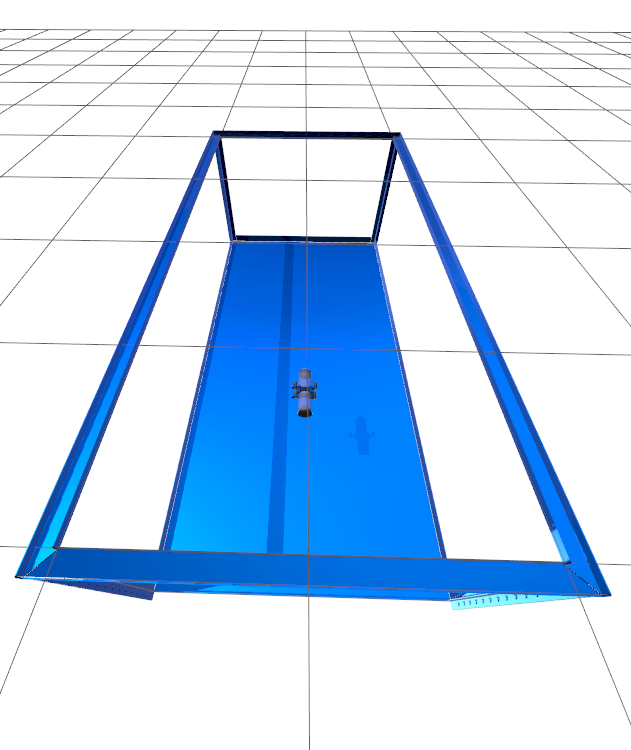
\includegraphics[width=0.4\textwidth]{images/04/gazebo.png}
    \quad\quad
    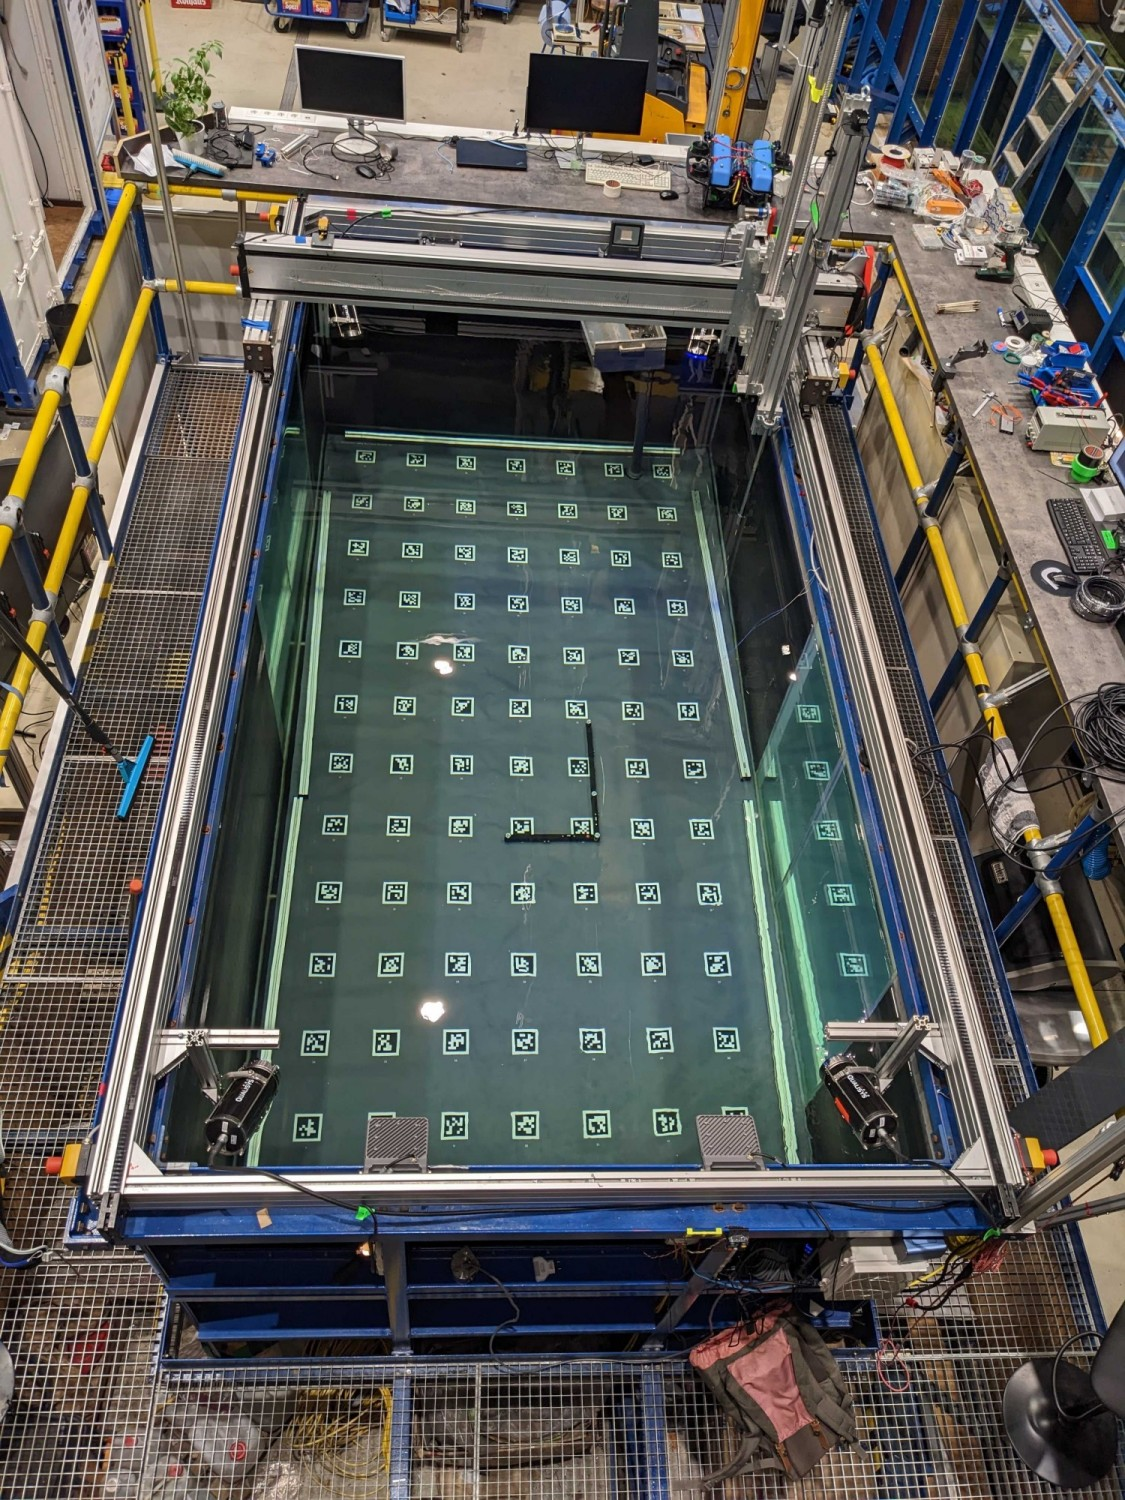
\includegraphics[width=0.4\textwidth]{images/04/roboquarium_tested_topview.jpg}
    \caption{Analysis setup for performance evaluations. Gazebo for simulation studies (\textit{left}) and top-view of the \textit{Roboquarium} underwater robot testbed (\textit{right}).}
    \label{fig:testbed_topview}
    \label{fig:analysis_setups}
\end{figure}
\subsection{Experimental Testbed}
Evaluating the performance of the proposed methodology in real-world experiments is an important step in the development process.
The physical experiments of this work have been conducted at the underwater robotics testing facilities \textit{Roboquarium} at the Institute of Mechanics and Ocean Engineering at TU Hamburg.
The dimensions of the used water basin are $4\times2\times1.5\,\mathrm{m}^3$.
\Cref{fig:testbed_topview} shows a photo of the testbed.
The tank is filled with fresh water that is continuously filtered and provides good visibility conditions as required by vision-based localization systems.
Furthermore, the tank floor is equipped with an array of AprilTag markers (Tag-Family 36h11, size $7.5$\,cm, $25$\,cm spacing in $X$-direction, $30$\,cm in $Y$-direction) to allow the usage of the onboard $\mu$AUV self-localization system described in \cite{Duecker20}.


\begin{figure}
    \centering
    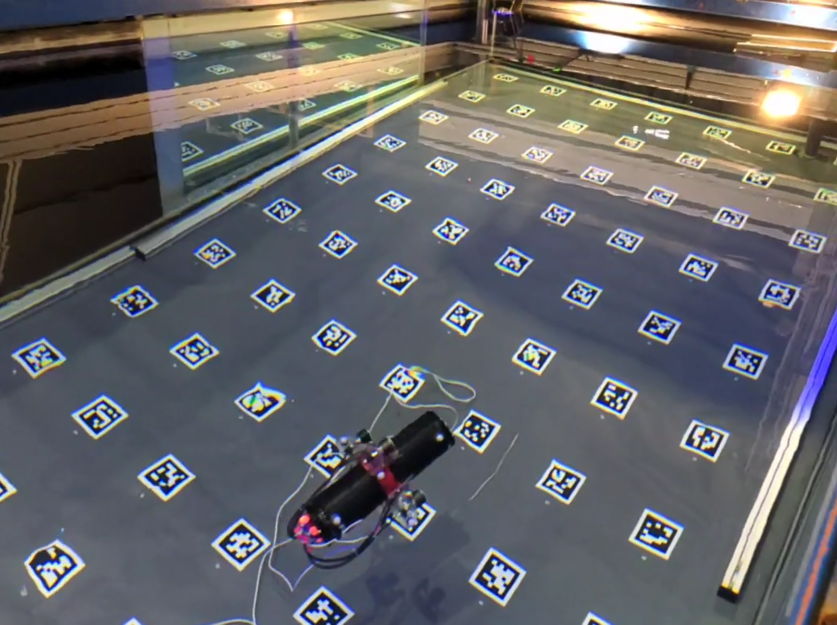
\includegraphics[width=0.7\textwidth]{images/04/hippo_in_tank.png}
    \caption{\textcolor{blue}{HippoCampus \ac{uauv} in experimental testbed.}}
    \label{fig:my_label}
\end{figure}


\subsubsection*{Qualisys Motion Capture System}
Recently, the Roboquarium testbed has been equipped with a professional underwater motion capture system to provide high-precision ground truth pose data of the tracked underwater objects.
The installed motion capture system features four \textit{Qualisys\,Miqus\,3} underwater cameras that are mounted into the corners of the water basin, as shown in \Cref{fig:testbed_topview}.
Prior to the experiment, the objects to be tracked, i.\,e. the \ac{uauv}, are equipped with multiple reflective markers, as depicted in \Cref{fig:hippo_with_marker}. 
In the current setup, the motion capture system provides 6-DOF data of pre-defined underwater objects at 100\,Hz, see also the 3D-overlay in \Cref{fig:qtm_3d} and the multi-camera reflection intensity view in \Cref{fig:qtm_intensity}.
Note that the motion captures system has been integrated into the Roboquarium ROS network.
This allows to use the data live within the experiment, e.\,g. as a pose data for the vehicle control loops.

Prior the experimental study, the motion capture system is calibrated to determine the camera positions with respect to the base frame origin. 
Moreover, the averaged residuals are computed using the software \textit{Qualisys Tracking Manager} (QTM).
The parameters are summarized in \Cref{tab:mocap_parameters}.


\begin{figure}
    \centering
    \includesvg[width=6cm]{images/04/hippo_with_markers}
    \caption{\textcolor{blue}{HippoCampus \ac{uauv} equipped with reflective markers. Note that the black tape is used to avoid reflections on the acrylic glas enclosure that can be misinterpreted as markers.}}
    \label{fig:hippo_with_marker}
\end{figure}


\begin{figure}
    \centering
    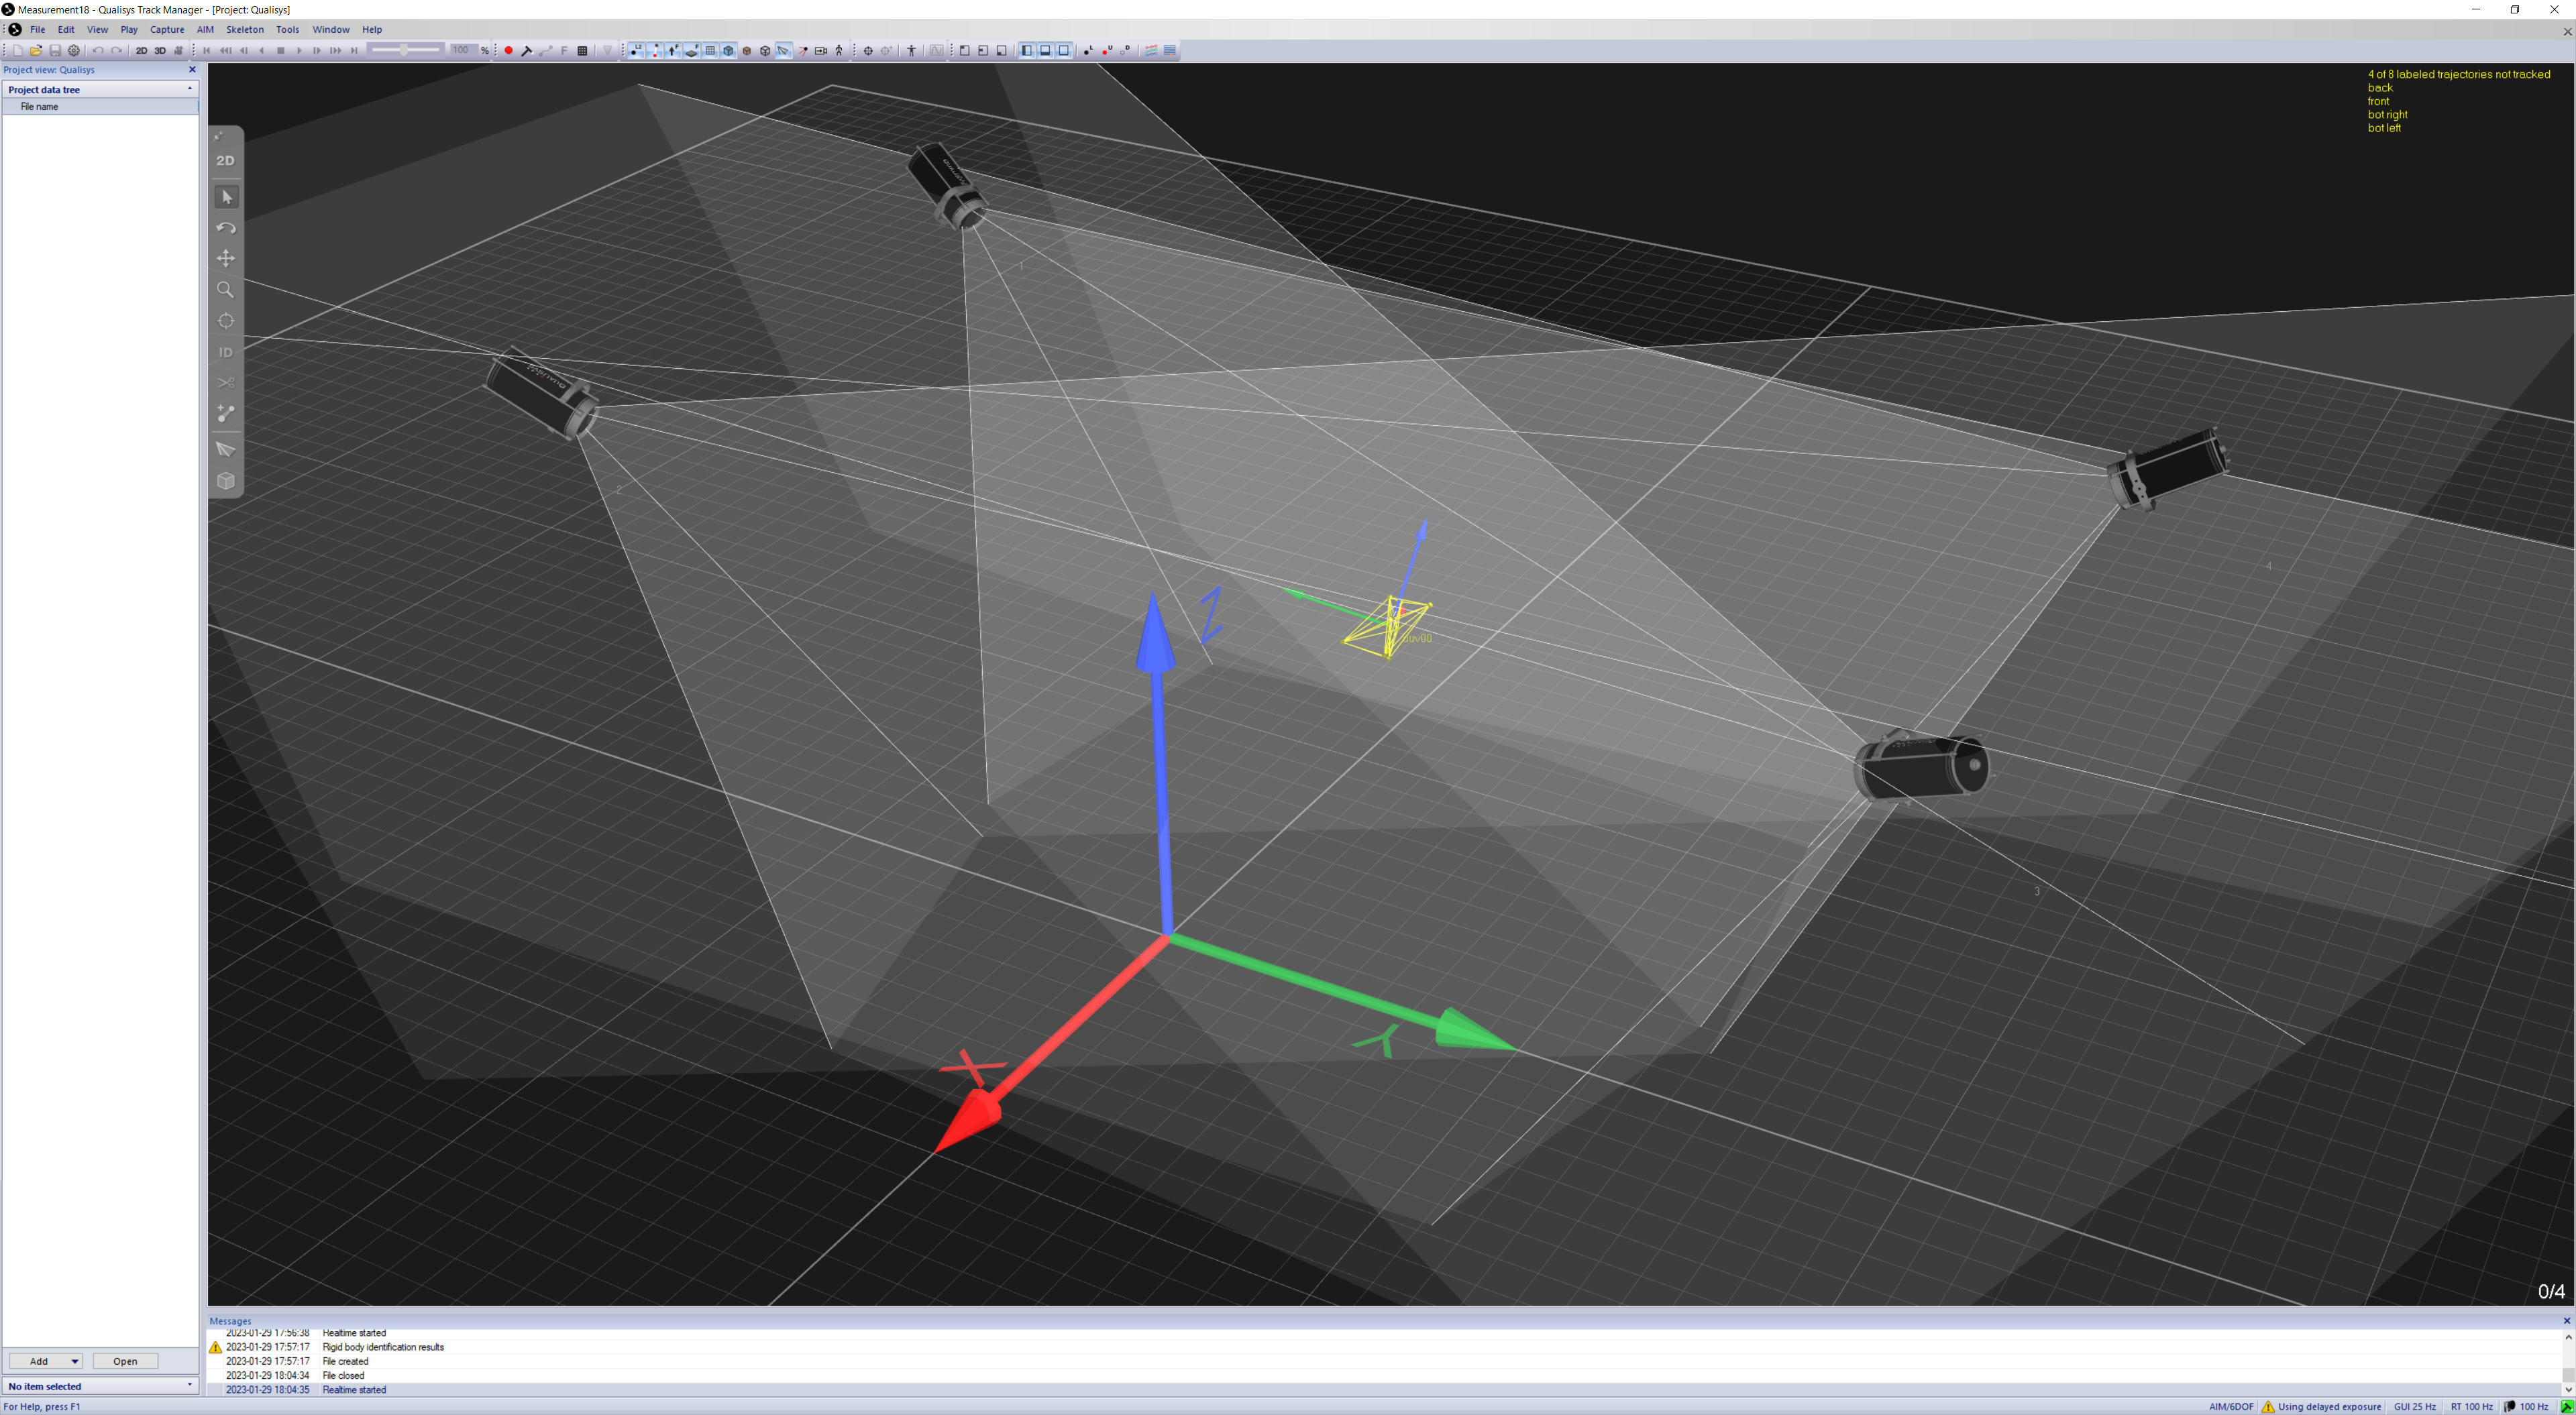
\includegraphics[width=0.9\textwidth]{images/04/qtm_3d_overlay.png}
    \caption{3D-overlay with tracked vehicle (yellow skeleton), the frame origin, and the four cameras provided by the Qualisys QTM software.}
    \label{fig:qtm_3d}
\end{figure}

\begin{figure}
    \centering
    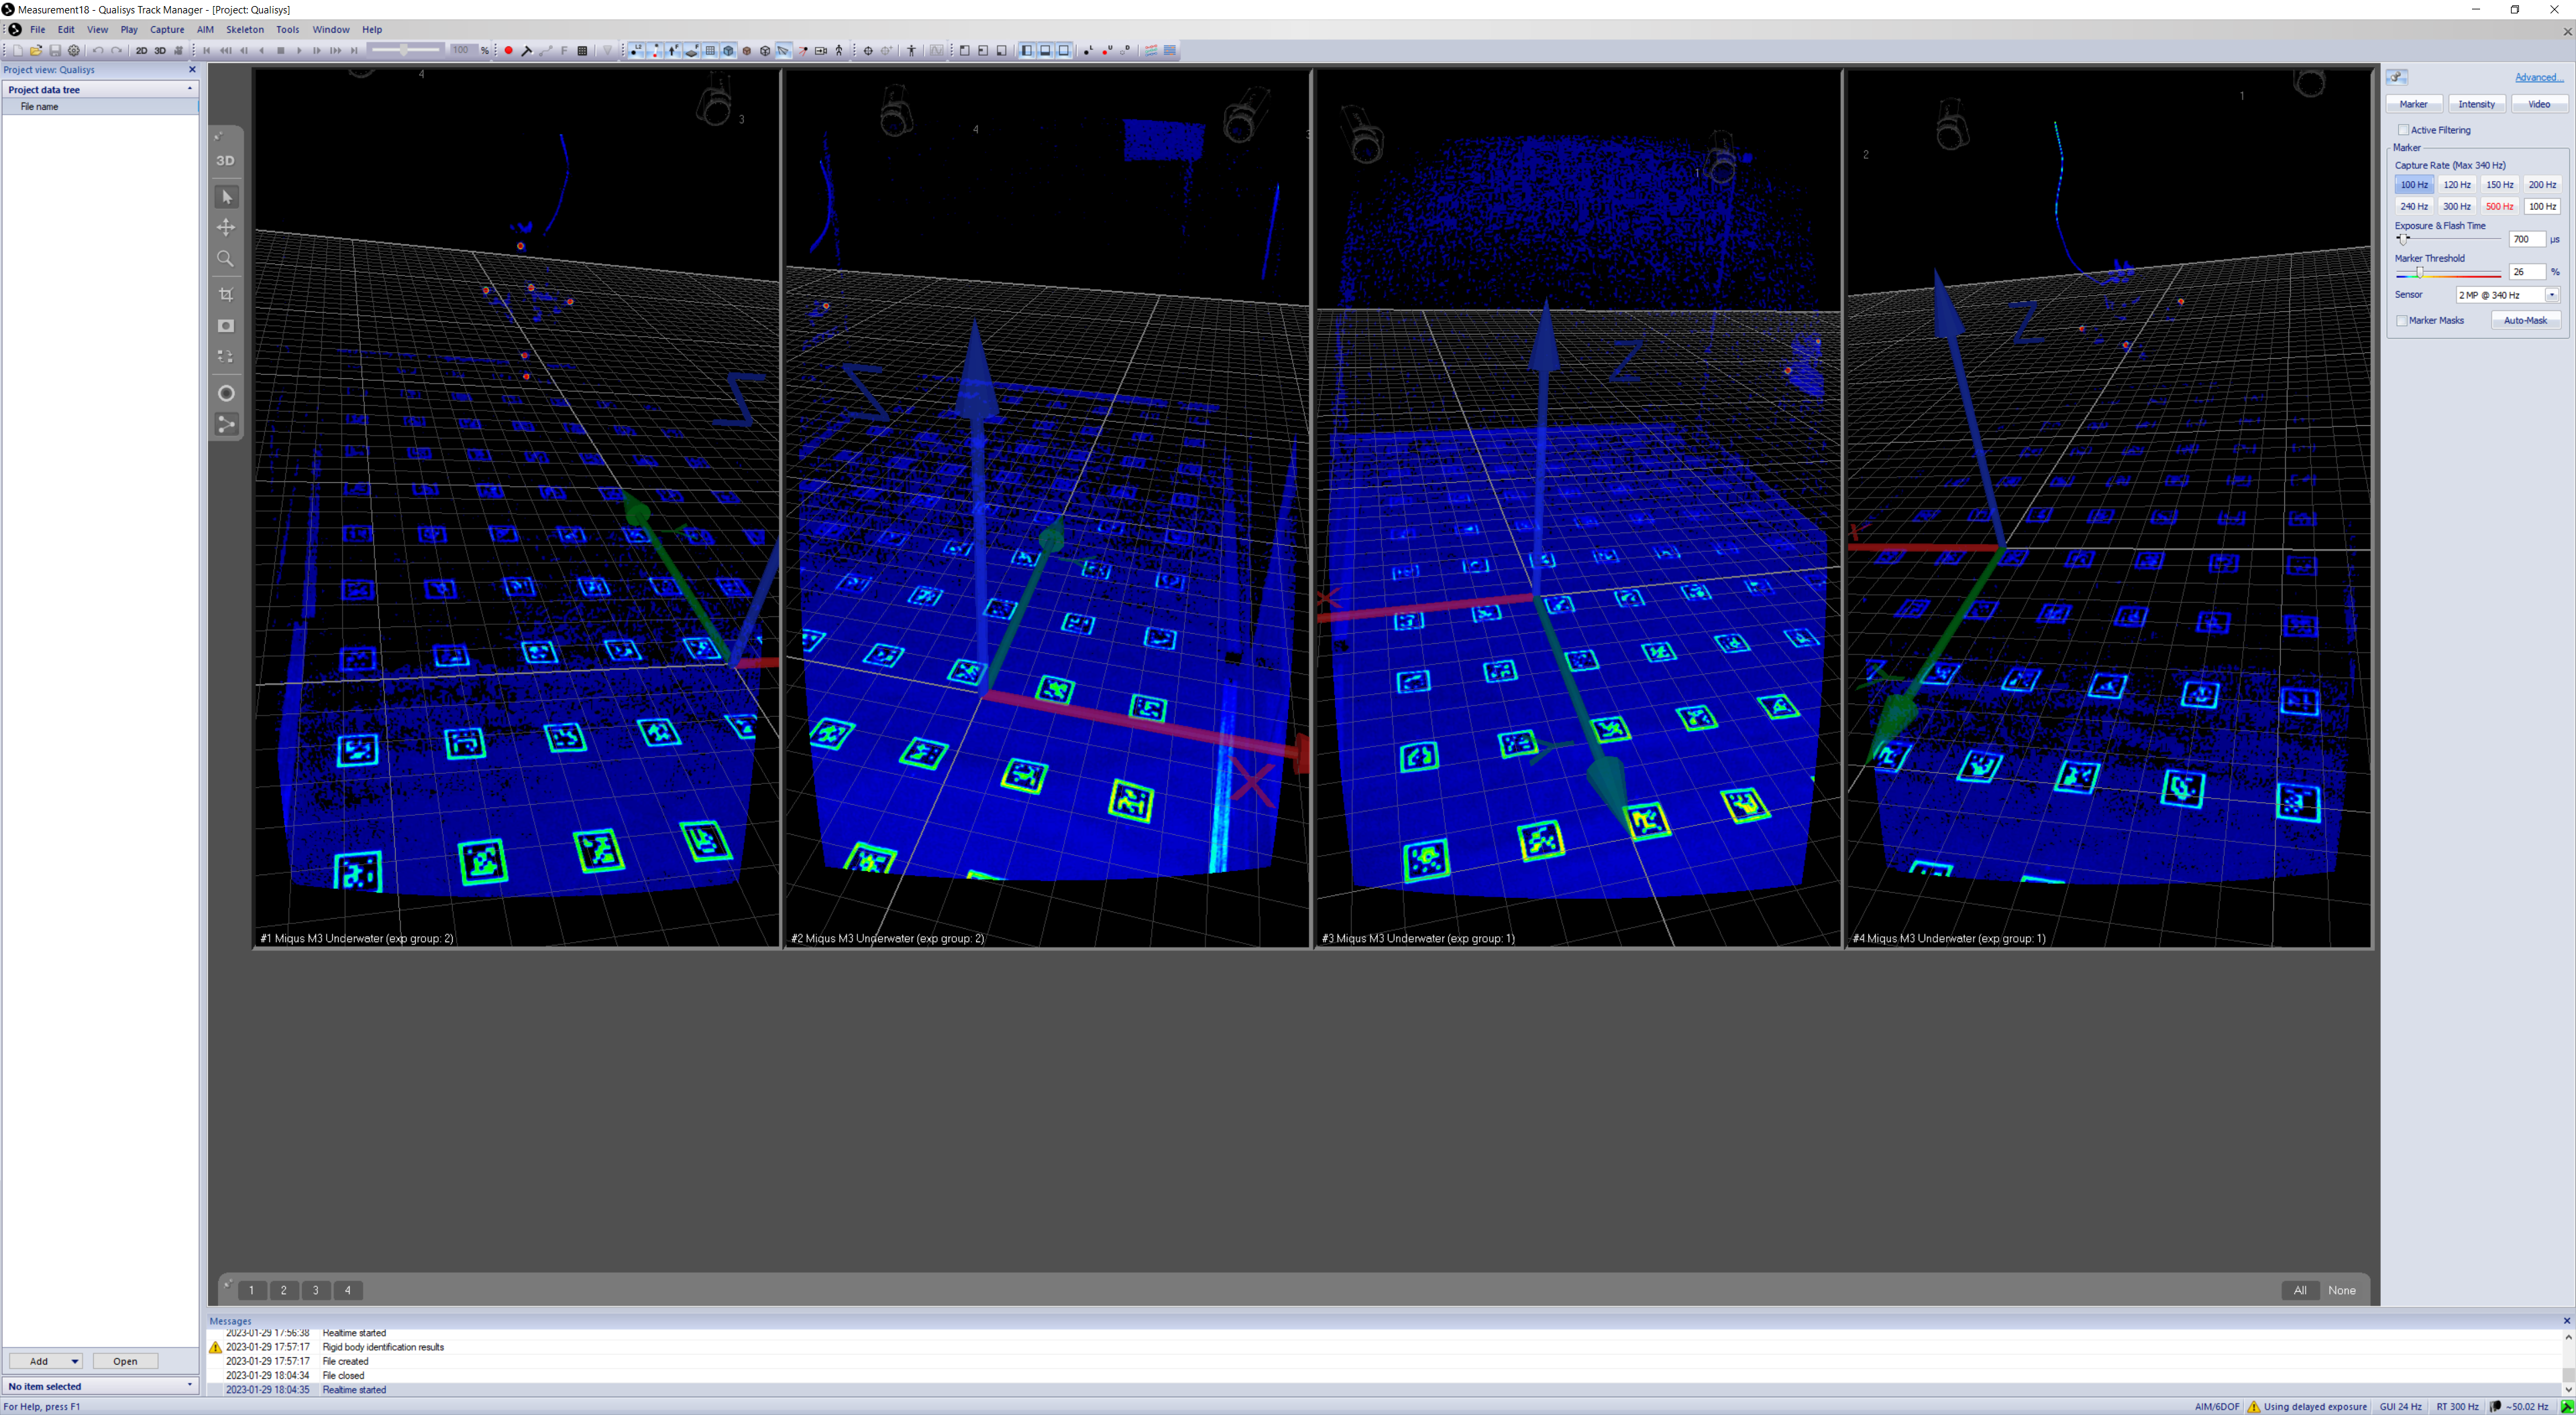
\includegraphics[width=0.9\textwidth]{images/04/qtm_multi_cam_intensity.png}
    \caption{Multi-camera view with reflective intensity from \textit{blue} (low intensity) to \textit{red} (high intensity).}
    \label{fig:qtm_intensity}
\end{figure}

% \begin{itemize}
%     \item Figure sketch - 4 cameras inside the tank (+ maybe screenshot from QTM?)
%     \item photo of sexy blue glowing cameras
%     \item photo of hippocampus with reflective markers
%     \item after conducting the QTM calibration procedure the estimated accuracy wihtin the calibration is XXXXXX according to the QTM calibration process.
% \end{itemize}

\begin{table}[]
        \caption{Calibration Parameters of Motion Capture System.}
		%\hspace*{-1.5cm}  % move table down (left in landscape) - tabular width: 
		\centering
		% change column width: >{\hsize=1.5\hsize\linewidth=\hsize}
		% >{\hsize=0.5\hsize\linewidth=\hsize}
		\begin{NiceTabular}
            {
            %%%%% Leider scheint die beste Methode wirklich hardgecodete Spaltenbreiten zu sein - hier am Ende rumspielen
            >{\centering\arraybackslash}m{2cm}  %
            >{\raggedleft\arraybackslash}m{1.7cm} % 
            >{\raggedleft\arraybackslash}m{1.7cm} %
            >{\centering\arraybackslash}m{1.7cm} %
            >{\centering\arraybackslash}m{2.2cm} %
            >{\centering\arraybackslash}m{2cm} %
            }
            \toprule
            %%%%%%%%%%% Top row - names of each columns
            Camera\,\# &  X\,(mm) & Y\,(mm) & Z\,(mm) & Calibration Points & Average Residual (mm) \\  
            \midrule 
            %%%%%%%% Beispiel
            01 & -1\,126.29 & -1\,346.14 & 1\,360.69 & 1\,891 & 0.5458 \\
            02 &     460.29 &  1\,357.67 & 1\,360.02 & 1\,584 & 0.6037\\
            03 &     483.47 &  2\,022.77 & 1\,350.27 & 1\,332 & 0.7383\\
            04 & -1\,055.28 &  2\,049.69 & 1\,326.27 & 1\,500 & 0.6270\\
            \bottomrule
		\end{NiceTabular}
		\label{tab:mocap_parameters}
\end{table}



\section{Body Rates Analysis}

In this section a brief analysis of the HippoCampus' body rates is given. Thereby, the assumption of instantaneously achievable body rates can be verified and put in a temporal context. Moreover, it is possible to determine an upper limit for feasible body rates, used in the trajectory module.

The first experiment is conducted without any controller. Only the angular rate around the vehicle's vertical axis $\exbody$ is examined, since the movement around the roll axis is not relevant for the trajectory tracking as stated in the previous chapter. The movement around $\eybody$ and $\ezbody$ can be assumed to be identical due to the symmetrical design of the vehicle. For the experiment, the vehicle is freely floating in the water of the tank depicted in \Cref{fig:testbed_topview}. The thrusters are then driven in saturation and the body rates are measured by the onboard \ac{imu}. The resulting body rate is shown in \Cref{fig:body-rate-saturation}.
\begin{figure}
	\centering
	\begin{tikzpicture}
		\begin{axis}[
			no markers,
			width=0.9\textwidth,
			height=7cm,
			grid=both,
			% ymax=1.5,
			xmax=0.7,
			enlarge x limits=false,
			xlabel={Time [s]},
			ylabel={Angular rate [\unit{rad/s}]},
			]
			\addplot+[thick] table [x=t, y=v_ang, col sep=comma] {data/lab/rates_saturation.csv};
		\end{axis}
	\end{tikzpicture}
	\caption{Angular rate for thrusters in saturation around the vehicle's vertical axis $\ezbody$. Maximum rate is ca. \unit[6.15]{rad/s}. \unit[63]{\%} of the maximum is reached around $\tau \approx \unit[0.3]{s}$.}
	\label{fig:body-rate-saturation}
\end{figure}
We observe a maximum achievable body rate of $\omega_{\max}\approx \unit[6.15]{rad/s}$, i.\,e. slightly below one rotation per second.
Furthermore, \unit[63]{\%} of the final rate are reached after \unit[0.3]{s}, which is equivalent of a time constnat $\tau = \unit[0.3]{s}$ for a first-order system.
Note that this experiment reflects a worst case scenario.
In general, we can expect to reach desired body rates faster, if a controller is used and the desired body rate is below the maximum possible.

In the second experiment, a body rate controller is deployed. The desired body rate is set to values between \unit[1]{rad/s} and \unit[4]{rad/s} and applied as step inputs to the system. The corresponding results are presented in \Cref{fig:body-rate-controlled}.
\begin{figure}
	\centering
	% This file was created with tikzplotlib v0.10.1.
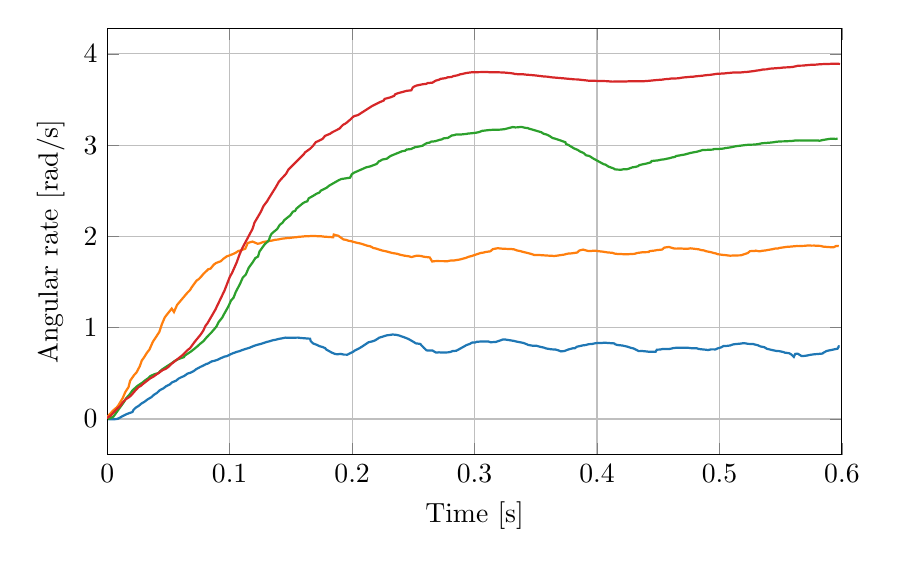
\begin{tikzpicture}

    \definecolor{crimson2143940}{RGB}{214,39,40}
    \definecolor{darkgray176}{RGB}{176,176,176}
    \definecolor{darkorange25512714}{RGB}{255,127,14}
    \definecolor{forestgreen4416044}{RGB}{44,160,44}
    \definecolor{steelblue31119180}{RGB}{31,119,180}
    
    \begin{axis}[
        no markers,
        width=0.9\textwidth,
        height=7cm,
        grid=both,
        % ymax=1.5,
        xmax=0.6,
        xmin=0.0,
        enlarge x limits=false,
        xlabel={Time [s]},
        ylabel={Angular rate [\unit{rad/s}]},
        ]
    \addplot [thick, steelblue31119180]
    table {%
    0.00100839138031006 0
    0.00170934200286865 -0.00297486782073975
    0.0060347318649292 -0.0022590160369873
    0.00820291042327881 0.00170981884002686
    0.0099865198135376 0.0111632347106934
    0.0118027925491333 0.0268406867980957
    0.0162643194198608 0.056022047996521
    0.0206483602523804 0.0773392915725708
    0.0215021371841431 0.100086569786072
    0.0231014490127563 0.122612476348877
    0.025739312171936 0.144909977912903
    0.0279875993728638 0.169950604438782
    0.0307220220565796 0.191496610641479
    0.0328801870346069 0.214525580406189
    0.0361002683639526 0.239649653434753
    0.0380610227584839 0.263952970504761
    0.0408321619033813 0.288434386253357
    0.0428565740585327 0.314947128295898
    0.0459061861038208 0.336158752441406
    0.0479105710983276 0.357527017593384
    0.0512164831161499 0.379925489425659
    0.0528401136398315 0.400899052619934
    0.0562864542007446 0.420705199241638
    0.0583771467208862 0.443774580955505
    0.0609358549118042 0.461017608642578
    0.0627588033676147 0.47038722038269
    0.0656512975692749 0.498075485229492
    0.0678802728652954 0.507119297981262
    0.0706249475479126 0.524978160858154
    0.0725613832473755 0.545421719551086
    0.0759495496749878 0.570120573043823
    0.0783511400222778 0.585171461105347
    0.0808194875717163 0.602779984474182
    0.0821772813796997 0.607456922531128
    0.0854929685592651 0.632565140724182
    0.0878051519393921 0.638497948646545
    0.0902107954025269 0.64976441860199
    0.092474102973938 0.664981961250305
    0.0958532094955444 0.684022903442383
    0.0979307889938354 0.690227150917053
    0.100520968437195 0.708064079284668
    0.102173686027527 0.718064188957214
    0.105814814567566 0.736100792884827
    0.107901692390442 0.743212103843689
    0.110125422477722 0.755027770996094
    0.112587809562683 0.766308307647705
    0.116363406181335 0.78153932094574
    0.118405699729919 0.79396641254425
    0.120801091194153 0.806039333343506
    0.122048497200012 0.811099052429199
    0.126386761665344 0.82666015625
    0.130804657936096 0.846328973770142
    0.132306456565857 0.851133704185486
    0.135558485984802 0.864486694335938
    0.137796998023987 0.869381308555603
    0.140339493751526 0.878643989562988
    0.142073273658752 0.882423281669617
    0.145782589912415 0.892211318016052
    0.148141264915466 0.890093684196472
    0.15095579624176 0.891763687133789
    0.152598738670349 0.891178250312805
    0.15576159954071 0.89221715927124
    0.157824873924255 0.888513326644897
    0.16134250164032 0.884587287902832
    0.165669798851013 0.880023956298828
    0.16617739200592 0.854219555854797
    0.168077349662781 0.828908801078796
    0.171183466911316 0.812732934951782
    0.17321503162384 0.798795580863953
    0.175943970680237 0.788997769355774
    0.178111433982849 0.77599036693573
    0.178760409355164 0.762779951095581
    0.183286070823669 0.728654503822327
    0.186215996742249 0.712475299835205
    0.188214182853699 0.709796905517578
    0.19062864780426 0.714000582695007
    0.193329215049744 0.705826044082642
    0.196190476417542 0.705385684967041
    0.198531031608582 0.72198748588562
    0.200776696205139 0.735857248306274
    0.201810717582703 0.747677326202393
    0.205991864204407 0.776113390922546
    0.208331704139709 0.795571684837341
    0.213487982749939 0.841542482376099
    0.216700196266174 0.851571202278137
    0.218412041664124 0.85966157913208
    0.221194386482239 0.881848573684692
    0.221752285957336 0.889320135116577
    0.228440165519714 0.917542457580566
    0.230732083320618 0.920764923095703
    0.233101487159729 0.926126480102539
    0.236084580421448 0.922364115715027
    0.238224387168884 0.915962934494019
    0.243476033210754 0.890963077545166
    0.245989680290222 0.877098083496094
    0.248237729072571 0.860488653182983
    0.252094149589539 0.829333186149597
    0.255567193031311 0.822996854782104
    0.258614897727966 0.780291557312012
    0.260794043540955 0.752848386764526
    0.261754631996155 0.750452041625977
    0.26547634601593 0.751882910728455
    0.268543124198914 0.727857708930969
    0.270976662635803 0.731044173240662
    0.272060751914978 0.729667186737061
    0.275431513786316 0.729022860527039
    0.278667807579041 0.730844259262085
    0.280753254890442 0.737185597419739
    0.281897664070129 0.744161605834961
    0.285097718238831 0.748141050338745
    0.291581988334656 0.796178102493286
    0.293277621269226 0.809411883354187
    0.296168684959412 0.82388162612915
    0.298308491706848 0.83966326713562
    0.3006831407547 0.839390158653259
    0.301677346229553 0.84600830078125
    0.305358290672302 0.849512457847595
    0.311160445213318 0.850459575653076
    0.313138365745544 0.841627478599548
    0.317123770713806 0.844023704528809
    0.319094061851501 0.852489709854126
    0.32316267490387 0.871326804161072
    0.325249552726746 0.870697855949402
    0.332188248634338 0.85597813129425
    0.333726763725281 0.850096344947815
    0.339949011802673 0.83368980884552
    0.342854380607605 0.818117737770081
    0.343639492988586 0.812349677085876
    0.347901225090027 0.802264213562012
    0.350756287574768 0.802004218101501
    0.353941321372986 0.790053248405457
    0.356600403785706 0.782565593719482
    0.358808398246765 0.772366523742676
    0.362640738487244 0.763930559158325
    0.366117835044861 0.761411190032959
    0.368320107460022 0.752909421920776
    0.37061083316803 0.741029381752014
    0.373421788215637 0.745360970497131
    0.376390337944031 0.761106133460999
    0.380616307258606 0.776779174804688
    0.381730914115906 0.774600625038147
    0.383579850196838 0.792365312576294
    0.388556361198425 0.807303905487061
    0.390717148780823 0.810739517211914
    0.3931964635849 0.820057392120361
    0.396137118339539 0.822973728179932
    0.398539423942566 0.8304603099823
    0.401487231254578 0.833885669708252
    0.403441309928894 0.832901477813721
    0.406464457511902 0.836586713790894
    0.408794283866882 0.833356142044067
    0.41416347026825 0.828585743904114
    0.41456139087677 0.821120738983154
    0.416312336921692 0.812203288078308
    0.418448090553284 0.808489203453064
    0.420760989189148 0.805390238761902
    0.424397826194763 0.794285893440247
    0.42757785320282 0.780317425727844
    0.429656863212585 0.774105072021484
    0.434104561805725 0.744065165519714
    0.437137722969055 0.744715690612793
    0.438931584358215 0.742703199386597
    0.442628502845764 0.736954092979431
    0.447851300239563 0.737119555473328
    0.448848605155945 0.759703397750854
    0.451128125190735 0.761006593704224
    0.453486561775208 0.766583561897278
    0.45928680896759 0.768448948860168
    0.459752202033997 0.77013885974884
    0.461273074150085 0.773001074790955
    0.46204149723053 0.776534676551819
    0.464168667793274 0.780021190643311
    0.468774914741516 0.781941056251526
    0.471100687980652 0.780011415481567
    0.473237633705139 0.782239079475403
    0.477282404899597 0.775926351547241
    0.481326699256897 0.775349974632263
    0.483119606971741 0.767593502998352
    0.48636519908905 0.762640595436096
    0.488498568534851 0.7600177526474
    0.490630984306335 0.75601851940155
    0.493261933326721 0.763331770896912
    0.496711373329163 0.762928366661072
    0.498636841773987 0.774785161018372
    0.501353979110718 0.785149097442627
    0.503172636032104 0.799256920814514
    0.506380081176758 0.801847219467163
    0.508643865585327 0.805820107460022
    0.51130223274231 0.818059921264648
    0.51317024230957 0.821281790733337
    0.517103910446167 0.826213598251343
    0.519394397735596 0.8306645154953
    0.521438121795654 0.828957319259644
    0.523238897323608 0.823907852172852
    0.527598142623901 0.821752071380615
    0.528661251068115 0.817279577255249
    0.531366586685181 0.808568477630615
    0.53343677520752 0.79549765586853
    0.536550760269165 0.787313342094421
    0.538809537887573 0.769576668739319
    0.543481349945068 0.75435996055603
    0.546495199203491 0.746192216873169
    0.54883337020874 0.743797063827515
    0.551697015762329 0.735660791397095
    0.553478717803955 0.727253675460815
    0.556817054748535 0.72132420539856
    0.558546543121338 0.708728194236755
    0.560757398605347 0.681100726127625
    0.561852216720581 0.713842391967773
    0.563910722732544 0.716067314147949
    0.566931247711182 0.691344857215881
    0.568951368331909 0.691075086593628
    0.571737289428711 0.696275949478149
    0.573312520980835 0.701359748840332
    0.576366424560547 0.70787239074707
    0.578424453735352 0.710601449012756
    0.584201097488403 0.717537760734558
    0.584590673446655 0.723655700683594
    0.587503910064697 0.745769381523132
    0.589487075805664 0.751557111740112
    0.596469879150391 0.771039605140686
    0.597395181655884 0.796517968177795
    0.598190069198608 0.797381401062012
    };
    \addplot [thick, darkorange25512714]
    table {%
    -0.00131130218505859 0
    0.00192379951477051 0.0506563186645508
    0.00493407249450684 0.0943666696548462
    0.00761985778808594 0.125157833099365
    0.00884270668029785 0.144006490707397
    0.0127365589141846 0.230819940567017
    0.0146951675415039 0.293288111686707
    0.0174276828765869 0.350194931030273
    0.0187280178070068 0.419081687927246
    0.021939754486084 0.481022596359253
    0.0239810943603516 0.511062264442444
    0.0266287326812744 0.578587532043457
    0.0283067226409912 0.641926407814026
    0.0298197269439697 0.669409275054932
    0.0325076580047607 0.727123498916626
    0.0345189571380615 0.761694192886353
    0.0372912883758545 0.84600818157196
    0.0425794124603271 0.954123973846436
    0.0446774959564209 1.03913450241089
    0.0469977855682373 1.11273539066315
    0.0487499237060547 1.14398717880249
    0.0527093410491943 1.20981633663177
    0.0545425415039062 1.17280697822571
    0.057056188583374 1.24982368946075
    0.0653548240661621 1.38164901733398
    0.0677163600921631 1.41427254676819
    0.0688169002532959 1.4393926858902
    0.072990894317627 1.51686215400696
    0.074796199798584 1.5326189994812
    0.0770676136016846 1.56529343128204
    0.0786211490631104 1.59079813957214
    0.082554817199707 1.64101922512054
    0.0843830108642578 1.6475989818573
    0.087083101272583 1.69173240661621
    0.0888576507568359 1.7091646194458
    0.0927934646606445 1.72923135757446
    0.0948352813720703 1.75507795810699
    0.0976195335388184 1.78171682357788
    0.0988509654998779 1.78725361824036
    0.102412939071655 1.80621778964996
    0.104735136032104 1.82006502151489
    0.107162714004517 1.84203612804413
    0.108806371688843 1.84654319286346
    0.112790822982788 1.86586809158325
    0.114763021469116 1.92869508266449
    0.117241382598877 1.93904912471771
    0.118722200393677 1.94383192062378
    0.122873067855835 1.92058563232422
    0.124542236328125 1.92447626590729
    0.127317905426025 1.93937134742737
    0.128759145736694 1.9429087638855
    0.134430646896362 1.95480954647064
    0.137399435043335 1.96473145484924
    0.139354467391968 1.96617865562439
    0.14232349395752 1.97530710697174
    0.144354343414307 1.97830736637115
    0.147257566452026 1.98317909240723
    0.148813009262085 1.98421895503998
    0.152410507202148 1.98985540866852
    0.154413938522339 1.99194920063019
    0.157013416290283 1.99750173091888
    0.158604621887207 1.99849009513855
    0.162869691848755 2.00387907028198
    0.164763689041138 2.0034613609314
    0.167211532592773 2.00555562973022
    0.169250726699829 2.00561428070068
    0.172373533248901 2.00262832641602
    0.174509763717651 2.0024995803833
    0.177400827407837 1.99778962135315
    0.17862343788147 1.99675524234772
    0.184549331665039 1.99147808551788
    0.18503737449646 2.02082395553589
    0.187453746795654 2.01192402839661
    0.188656568527222 2.00854134559631
    0.192923069000244 1.96764981746674
    0.194900989532471 1.96354067325592
    0.197121381759644 1.95288336277008
    0.198583364486694 1.95049726963043
    0.202783584594727 1.93467032909393
    0.207347393035889 1.92129170894623
    0.208871126174927 1.91501724720001
    0.212532043457031 1.89853990077972
    0.214849948883057 1.89277637004852
    0.217444658279419 1.87359154224396
    0.219091415405273 1.86934864521027
    0.224791049957275 1.84540903568268
    0.227758884429932 1.83756577968597
    0.22881555557251 1.83383023738861
    0.232588291168213 1.81964480876923
    0.237077236175537 1.80961883068085
    0.238877296447754 1.80093657970428
    0.243008852005005 1.78914797306061
    0.244711637496948 1.78640568256378
    0.24683666229248 1.78139626979828
    0.248546600341797 1.77449119091034
    0.252754211425781 1.79019606113434
    0.255362749099731 1.78751695156097
    0.256657600402832 1.78514444828033
    0.258007287979126 1.77980816364288
    0.259816408157349 1.77588474750519
    0.263429880142212 1.77031624317169
    0.265395402908325 1.72599983215332
    0.267714500427246 1.73002588748932
    0.268916845321655 1.73066008090973
    0.272976636886597 1.72993099689484
    0.274898767471313 1.72990739345551
    0.276918888092041 1.72766005992889
    0.277820348739624 1.72903645038605
    0.279919624328613 1.73548686504364
    0.283508539199829 1.73784649372101
    0.288039207458496 1.74791383743286
    0.288777351379395 1.75043451786041
    0.293084621429443 1.76622438430786
    0.295062065124512 1.7774019241333
    0.298104047775269 1.78767895698547
    0.29919171333313 1.79340922832489
    0.304800510406494 1.81870853900909
    0.307791233062744 1.82499325275421
    0.308619260787964 1.82921493053436
    0.312866449356079 1.83756983280182
    0.314992189407349 1.86169564723969
    0.318876028060913 1.87148308753967
    0.322620153427124 1.86636471748352
    0.32471489906311 1.86527466773987
    0.327189207077026 1.86344277858734
    0.328771591186523 1.86406433582306
    0.332293748855591 1.85897421836853
    0.334635972976685 1.84708774089813
    0.337692022323608 1.83903777599335
    0.338651180267334 1.83450520038605
    0.344757556915283 1.81430530548096
    0.347093820571899 1.80550718307495
    0.348552227020264 1.7978857755661
    0.352335691452026 1.7971556186676
    0.360037803649902 1.79036164283752
    0.363295316696167 1.78856635093689
    0.364935398101807 1.78596913814545
    0.367775201797485 1.79082047939301
    0.36871075630188 1.79291045665741
    0.373251914978027 1.80161035060883
    0.374792098999023 1.80781042575836
    0.376936674118042 1.81382203102112
    0.378574848175049 1.81428146362305
    0.383755922317505 1.82374131679535
    0.385621547698975 1.84664046764374
    0.388630628585815 1.85647130012512
    0.392818927764893 1.8407506942749
    0.394803524017334 1.84101569652557
    0.397534608840942 1.84468638896942
    0.398593425750732 1.84451031684875
    0.402793645858765 1.83651924133301
    0.404784440994263 1.83386087417603
    0.408705234527588 1.82517945766449
    0.412586450576782 1.82112419605255
    0.41461706161499 1.81207549571991
    0.416978359222412 1.80821442604065
    0.418598413467407 1.80860245227814
    0.422294616699219 1.80535459518433
    0.424790620803833 1.80540060997009
    0.430798292160034 1.81015741825104
    0.43276047706604 1.81919813156128
    0.436633348464966 1.82624554634094
    0.442230224609375 1.82982587814331
    0.442840337753296 1.8392071723938
    0.444683790206909 1.84241628646851
    0.447497129440308 1.84665966033936
    0.448571443557739 1.85019254684448
    0.453107357025146 1.85662448406219
    0.454980850219727 1.87799978256226
    0.458618879318237 1.88557171821594
    0.46306848526001 1.86787569522858
    0.464597940444946 1.86692416667938
    0.467304944992065 1.86820757389069
    0.468673229217529 1.86784708499908
    0.472763299942017 1.8652366399765
    0.474699020385742 1.86664307117462
    0.476266860961914 1.8702312707901
    0.479105472564697 1.86593639850616
    0.483132839202881 1.85893738269806
    0.485044002532959 1.85125744342804
    0.48746395111084 1.84711539745331
    0.488699674606323 1.83945071697235
    0.493084907531738 1.82793152332306
    0.495161294937134 1.81956994533539
    0.497339487075806 1.81338131427765
    0.498535871505737 1.80600392818451
    0.50272798538208 1.79824268817902
    0.504963159561157 1.79581391811371
    0.507137537002563 1.79173219203949
    0.508659362792969 1.78963792324066
    0.512770414352417 1.79196751117706
    0.517638683319092 1.79362261295319
    0.518078565597534 1.79612243175507
    0.522958040237427 1.81771266460419
    0.525027275085449 1.83948338031769
    0.529008388519287 1.84159064292908
    0.52937912940979 1.8448588848114
    0.532840251922607 1.83696138858795
    0.534844160079956 1.84350049495697
    0.537458896636963 1.84656393527985
    0.538737773895264 1.8503338098526
    0.543137788772583 1.86044728755951
    0.54517674446106 1.86714398860931
    0.547930479049683 1.86920464038849
    0.548810005187988 1.87441313266754
    0.552643775939941 1.88150060176849
    0.554803133010864 1.88621628284454
    0.557920932769775 1.88900077342987
    0.558965921401978 1.89040195941925
    0.563070774078369 1.89533150196075
    0.564570903778076 1.8942939043045
    0.567825078964233 1.89683258533478
    0.569269895553589 1.8973776102066
    0.572980880737305 1.90269124507904
    0.574981451034546 1.89969098567963
    0.577449083328247 1.90023744106293
    0.579171895980835 1.89847815036774
    0.582269430160522 1.89698612689972
    0.584804534912109 1.88894188404083
    0.586469173431396 1.88701641559601
    0.589634656906128 1.88367021083832
    0.593177556991577 1.88132512569427
    0.595215320587158 1.89551246166229
    0.597409009933472 1.8947639465332
    };
    \addplot [thick, forestgreen4416044]
    table {%
    0.000681638717651367 0
    0.00345873832702637 0.0162497758865356
    0.00517511367797852 0.0278317928314209
    0.01346755027771 0.182381510734558
    0.0154781341552734 0.227526187896729
    0.0185041427612305 0.27259635925293
    0.0205926895141602 0.313456773757935
    0.0246875286102295 0.362778425216675
    0.0287501811981201 0.398780107498169
    0.0310473442077637 0.424405455589294
    0.0336039066314697 0.448204874992371
    0.0351784229278564 0.470171093940735
    0.0386786460876465 0.491460800170898
    0.0418181419372559 0.504035353660583
    0.0432963371276855 0.525519847869873
    0.0449559688568115 0.544305682182312
    0.050837516784668 0.596061229705811
    0.0532708168029785 0.617340564727783
    0.0553109645843506 0.638011693954468
    0.0584917068481445 0.658659696578979
    0.0626599788665771 0.678431987762451
    0.0634257793426514 0.695814728736877
    0.0647780895233154 0.70732855796814
    0.0685293674468994 0.740913033485413
    0.0735137462615967 0.79467248916626
    0.075883150100708 0.824188947677612
    0.0787711143493652 0.855002164840698
    0.0810775756835938 0.893170356750488
    0.0849602222442627 0.946509003639221
    0.0891668796539307 1.01238226890564
    0.0910241603851318 1.06248438358307
    0.0941240787506104 1.11434316635132
    0.0951175689697266 1.14217877388
    0.0989973545074463 1.23415589332581
    0.101139068603516 1.29909539222717
    0.10321307182312 1.32950615882874
    0.104989051818848 1.39194750785828
    0.108473539352417 1.48045992851257
    0.110705852508545 1.54894995689392
    0.11314868927002 1.58172750473022
    0.11559271812439 1.65762424468994
    0.118741989135742 1.71580648422241
    0.120979785919189 1.7633068561554
    0.12316370010376 1.78003120422363
    0.124377965927124 1.83546733856201
    0.128607988357544 1.91423773765564
    0.131844758987427 1.95391869544983
    0.133371114730835 2.00928521156311
    0.1343674659729 2.03208041191101
    0.138786792755127 2.08122777938843
    0.140909910202026 2.12706279754639
    0.143298387527466 2.15235900878906
    0.1446373462677 2.17935800552368
    0.149485111236572 2.23132157325745
    0.151612520217896 2.27129721641541
    0.153413057327271 2.28034472465515
    0.154642581939697 2.30695915222168
    0.15942645072937 2.36009359359741
    0.161232471466064 2.37579083442688
    0.163352489471436 2.38499093055725
    0.164575338363647 2.4181067943573
    0.168453693389893 2.4471697807312
    0.170790433883667 2.46729350090027
    0.173294067382812 2.48159503936768
    0.174502849578857 2.50280952453613
    0.179256439208984 2.53418827056885
    0.181071996688843 2.55528831481934
    0.188729047775269 2.61395382881165
    0.191052198410034 2.62910461425781
    0.198361396789551 2.64422392845154
    0.199723720550537 2.68128895759583
    0.201287269592285 2.69701147079468
    0.211574792861938 2.75804376602173
    0.214711666107178 2.76740765571594
    0.220107793807983 2.79470181465149
    0.221856355667114 2.82278275489807
    0.2231764793396 2.82996010780334
    0.224536657333374 2.84172511100769
    0.228399753570557 2.85278248786926
    0.231292963027954 2.88157057762146
    0.240879058837891 2.93408846855164
    0.24326753616333 2.93942713737488
    0.244561910629272 2.95245051383972
    0.248085975646973 2.95796895027161
    0.251393795013428 2.97828483581543
    0.253414630889893 2.98227953910828
    0.257775068283081 2.99519681930542
    0.258299112319946 3.00308322906494
    0.261265754699707 3.02452921867371
    0.263275146484375 3.0280385017395
    0.264523983001709 3.03907608985901
    0.267808675765991 3.04326796531677
    0.27151346206665 3.05908751487732
    0.27335000038147 3.06411385536194
    0.274743795394897 3.07490682601929
    0.278305292129517 3.08047270774841
    0.281309604644775 3.10594439506531
    0.283552646636963 3.11122155189514
    0.284668922424316 3.11628127098083
    0.288361787796021 3.11673831939697
    0.291332960128784 3.12097859382629
    0.293344497680664 3.12347197532654
    0.294686794281006 3.12754726409912
    0.296579122543335 3.12974381446838
    0.301003932952881 3.13601446151733
    0.30383563041687 3.14458465576172
    0.306251049041748 3.15742993354797
    0.308690309524536 3.16098117828369
    0.310834169387817 3.16467499732971
    0.314488410949707 3.16851663589478
    0.318009376525879 3.16856741905212
    0.321422338485718 3.17121386528015
    0.32456636428833 3.1760573387146
    0.33120059967041 3.19896101951599
    0.333288431167603 3.1949737071991
    0.334444522857666 3.19543504714966
    0.33834171295166 3.20045709609985
    0.341346502304077 3.19038510322571
    0.343427419662476 3.187659740448
    0.344516038894653 3.18116974830627
    0.346605062484741 3.1734733581543
    0.354484796524048 3.14216375350952
    0.356130599975586 3.12700271606445
    0.359317064285278 3.11456489562988
    0.361562252044678 3.09822964668274
    0.363775730133057 3.07833886146545
    0.365950107574463 3.07116365432739
    0.374130725860596 3.03353261947632
    0.374679803848267 3.0135555267334
    0.376514196395874 3.00381088256836
    0.381369590759277 2.96402668952942
    0.384198665618896 2.94890904426575
    0.385980844497681 2.93250966072083
    0.389056205749512 2.91430902481079
    0.391077518463135 2.8896336555481
    0.393778324127197 2.88162064552307
    0.396517992019653 2.85745882987976
    0.405406951904297 2.79205632209778
    0.406928062438965 2.78725385665894
    0.409267425537109 2.76617074012756
    0.413715124130249 2.7443675994873
    0.414500951766968 2.73625206947327
    0.416755676269531 2.73274230957031
    0.4195876121521 2.73131608963013
    0.421659231185913 2.73638415336609
    0.424237251281738 2.73608303070068
    0.426060438156128 2.74332118034363
    0.428974866867065 2.75781273841858
    0.431177616119385 2.7616331577301
    0.43333101272583 2.76951575279236
    0.434549570083618 2.78116250038147
    0.436518907546997 2.78838872909546
    0.440309047698975 2.79869699478149
    0.443863153457642 2.81210279464722
    0.444582223892212 2.82631540298462
    0.446475028991699 2.82947015762329
    0.449668169021606 2.83370971679688
    0.452086448669434 2.8410382270813
    0.455138444900513 2.84584951400757
    0.456025123596191 2.84883832931519
    0.459107637405396 2.85732364654541
    0.461352586746216 2.86611843109131
    0.463497400283813 2.8713436126709
    0.464608430862427 2.88190317153931
    0.466571807861328 2.88614559173584
    0.471800327301025 2.89854192733765
    0.476538419723511 2.91610288619995
    0.481515645980835 2.92858505249023
    0.483754396438599 2.93688058853149
    0.48598313331604 2.94645690917969
    0.494689464569092 2.9521656036377
    0.495564937591553 2.95778131484985
    0.49618124961853 2.95707416534424
    0.499475240707397 2.95886135101318
    0.501980781555176 2.96147680282593
    0.50377893447876 2.96467590332031
    0.504615068435669 2.96837139129639
    0.506465435028076 2.97115421295166
    0.509483814239502 2.9775333404541
    0.513323783874512 2.98864912986755
    0.514477252960205 2.99107241630554
    0.516490459442139 2.9935462474823
    0.519870519638062 2.99981570243835
    0.521757125854492 3.0025908946991
    0.524247169494629 3.00523209571838
    0.52910852432251 3.00725364685059
    0.533421516418457 3.01678276062012
    0.534607648849487 3.02156734466553
    0.536732912063599 3.02335453033447
    0.541221857070923 3.0280544757843
    0.544243574142456 3.03240489959717
    0.545939683914185 3.03691339492798
    0.549405336380005 3.04138970375061
    0.553305149078369 3.04237651824951
    0.554795265197754 3.0437376499176
    0.556653499603271 3.04482507705688
    0.559740304946899 3.04747867584229
    0.561562776565552 3.0508279800415
    0.565251588821411 3.05279922485352
    0.566527605056763 3.052570104599
    0.571488380432129 3.05123162269592
    0.574214696884155 3.05139851570129
    0.581060409545898 3.05047631263733
    0.581631422042847 3.04830074310303
    0.584261178970337 3.05669546127319
    0.586019515991211 3.06044840812683
    0.589286088943481 3.06808853149414
    0.591400623321533 3.0714955329895
    0.593610525131226 3.07016730308533
    0.594788551330566 3.06916213035583
    0.596487998962402 3.07068634033203
    };
    \addplot [thick, crimson2143940]
    table {%
    -0.00170993804931641 0
    0.0026850700378418 0.0354610681533813
    0.00790214538574219 0.11038875579834
    0.0107574462890625 0.143845677375793
    0.0125904083251953 0.181577682495117
    0.0153663158416748 0.218361139297485
    0.0176980495452881 0.23790979385376
    0.0195083618164062 0.258614301681519
    0.0228898525238037 0.310983657836914
    0.0255389213562012 0.349045515060425
    0.0275428295135498 0.364142417907715
    0.0296056270599365 0.388603448867798
    0.0350174903869629 0.444669246673584
    0.0379195213317871 0.466175675392151
    0.0403194427490234 0.48979127407074
    0.0418713092803955 0.502832889556885
    0.0453739166259766 0.537086725234985
    0.0476410388946533 0.548727750778198
    0.0500481128692627 0.571954011917114
    0.0517361164093018 0.59600555896759
    0.0617661476135254 0.702831029891968
    0.065556526184082 0.755048036575317
    0.0676114559173584 0.77561891078949
    0.0718355178833008 0.85287606716156
    0.0759620666503906 0.918946504592896
    0.0784170627593994 0.966806411743164
    0.0802454948425293 1.02107274532318
    0.0819375514984131 1.05022025108337
    0.0882000923156738 1.19505882263184
    0.0957386493682861 1.40588474273682
    0.100259780883789 1.56161713600159
    0.10184121131897 1.59706354141235
    0.105803966522217 1.71748661994934
    0.108167409896851 1.80633139610291
    0.110366106033325 1.87348914146423
    0.118637800216675 2.08178758621216
    0.120306730270386 2.15169167518616
    0.12560248374939 2.27331519126892
    0.127647638320923 2.33391213417053
    0.130566596984863 2.38512873649597
    0.131832599639893 2.41459131240845
    0.137878656387329 2.54423260688782
    0.14015793800354 2.59876656532288
    0.141607046127319 2.62186002731323
    0.146042823791504 2.68632745742798
    0.147955417633057 2.73233914375305
    0.160516977310181 2.9003541469574
    0.161531686782837 2.92081332206726
    0.165688991546631 2.96127247810364
    0.168100118637085 2.99349093437195
    0.170352697372437 3.0335419178009
    0.172579765319824 3.04681754112244
    0.175832509994507 3.0683958530426
    0.177910327911377 3.10253405570984
    0.182090282440186 3.12574934959412
    0.183551788330078 3.14012598991394
    0.189691543579102 3.18178486824036
    0.190093278884888 3.18848919868469
    0.192498922348022 3.2221143245697
    0.194920063018799 3.24018836021423
    0.198550462722778 3.28109288215637
    0.200458288192749 3.30711054801941
    0.201863050460815 3.31917691230774
    0.204830646514893 3.33040261268616
    0.216466188430786 3.43039011955261
    0.22275710105896 3.47215437889099
    0.225869178771973 3.48987030982971
    0.226548671722412 3.5072238445282
    0.231378078460693 3.52469229698181
    0.234339952468872 3.54055142402649
    0.235098838806152 3.5571277141571
    0.237368822097778 3.56944394111633
    0.244637489318848 3.59577393531799
    0.248391389846802 3.6015408039093
    0.249499320983887 3.63159203529358
    0.250611543655396 3.64229512214661
    0.252532958984375 3.65350127220154
    0.257787466049194 3.66809725761414
    0.260323286056519 3.67150664329529
    0.26171612739563 3.68084692955017
    0.265516996383667 3.68499732017517
    0.26823902130127 3.70719122886658
    0.270786285400391 3.71670794487
    0.272385120391846 3.7271888256073
    0.276532649993896 3.73533129692078
    0.277801752090454 3.74311900138855
    0.281320333480835 3.74822354316711
    0.282503366470337 3.75601744651794
    0.286118984222412 3.76584124565125
    0.288255453109741 3.77654123306274
    0.290139436721802 3.78094887733459
    0.292814493179321 3.78986263275146
    0.296170949935913 3.79661178588867
    0.297894716262817 3.79897308349609
    0.301034688949585 3.80045294761658
    0.302831888198853 3.80031633377075
    0.306079626083374 3.8012318611145
    0.310259342193604 3.80175924301147
    0.312631368637085 3.79935503005981
    0.320407629013062 3.79815602302551
    0.32372260093689 3.79639506340027
    0.32476544380188 3.79535055160522
    0.329822301864624 3.78900980949402
    0.332042694091797 3.78434443473816
    0.332851886749268 3.78080224990845
    0.335773706436157 3.77747392654419
    0.33978533744812 3.77693605422974
    0.341017723083496 3.77428245544434
    0.345792055130005 3.76926803588867
    0.348349809646606 3.76603698730469
    0.351176977157593 3.76209950447083
    0.357090950012207 3.751953125
    0.359075307846069 3.75131845474243
    0.362417459487915 3.74472951889038
    0.363545417785645 3.74302291870117
    0.372896909713745 3.73229956626892
    0.381820917129517 3.72103190422058
    0.383833885192871 3.72100400924683
    0.387479066848755 3.71530842781067
    0.389488220214844 3.71254372596741
    0.393406391143799 3.70640397071838
    0.396294832229614 3.70506286621094
    0.398316621780396 3.70516896247864
    0.402444839477539 3.70368194580078
    0.408086061477661 3.70160698890686
    0.410880565643311 3.69819712638855
    0.412631273269653 3.69646525382996
    0.415969848632812 3.69769883155823
    0.418283939361572 3.69735193252563
    0.420626640319824 3.69880032539368
    0.421767950057983 3.69875764846802
    0.423385858535767 3.69852447509766
    0.428246974945068 3.70101428031921
    0.433469533920288 3.70033621788025
    0.436256885528564 3.70141553878784
    0.438431262969971 3.7014799118042
    0.442599058151245 3.70565867424011
    0.448247909545898 3.71324729919434
    0.451088428497314 3.71645617485046
    0.452744245529175 3.71748566627502
    0.455817937850952 3.7237491607666
    0.458195447921753 3.72546815872192
    0.460537433624268 3.73038935661316
    0.461821556091309 3.73043465614319
    0.463372468948364 3.73097109794617
    0.466465473175049 3.73300957679749
    0.468231916427612 3.73771190643311
    0.470883369445801 3.74271774291992
    0.472375392913818 3.74390006065369
    0.475903749465942 3.74889492988586
    0.47835373878479 3.7502863407135
    0.481201410293579 3.75591135025024
    0.482644081115723 3.75695586204529
    0.486340999603271 3.76186275482178
    0.488237380981445 3.76600050926208
    0.490806818008423 3.76941299438477
    0.492560386657715 3.77099943161011
    0.497973680496216 3.78218388557434
    0.503542423248291 3.78573250770569
    0.506030321121216 3.78992509841919
    0.508151769638062 3.7921359539032
    0.510576248168945 3.79533267021179
    0.512639760971069 3.7960991859436
    0.515645265579224 3.7964334487915
    0.517815351486206 3.79764842987061
    0.521272897720337 3.80239343643188
    0.522383213043213 3.80273485183716
    0.52812385559082 3.81230616569519
    0.530418157577515 3.81783652305603
    0.532803297042847 3.82167553901672
    0.53587532043457 3.83017778396606
    0.538280248641968 3.83081388473511
    0.540764570236206 3.83792018890381
    0.550590753555298 3.8479368686676
    0.552342891693115 3.85150980949402
    0.556367874145508 3.85356187820435
    0.559761047363281 3.85729908943176
    0.56299901008606 3.86641550064087
    0.563472986221313 3.86911153793335
    0.56649374961853 3.87182068824768
    0.568233013153076 3.87215828895569
    0.570712327957153 3.87621092796326
    0.572246074676514 3.87770342826843
    0.576054334640503 3.88230466842651
    0.578335285186768 3.88230991363525
    0.582436800003052 3.88741159439087
    0.585874795913696 3.88921403884888
    0.588076829910278 3.88985085487366
    0.590672969818115 3.89126968383789
    0.592339754104614 3.89194583892822
    0.596213579177856 3.89206957817078
    0.598446130752563 3.89065265655518
    };
    \end{axis}
    
    \end{tikzpicture}
    
	\caption{Angular rates with active rate controller. First-order time constant can be assumed in the magnitude of $\tau=\unit[0.1]{s}$}.
	\label{fig:body-rate-controlled}
\end{figure}
The body rates are reached significantly faster than in the first experiment without controller.
The first-order time constant can be estimated to be in the vicinity of $\tau=\unit[0.1]{s}$. Still, it takes considerable time to reach the desired body rates, which should be noted for future design of control modules.

\section{Computational Performance}
For the trajectory generation and implicit feedback control scheme, the computation time required for sampling new trajectories and check their feasibility with respect to the dynamic and translational constraints, is crucial. The more trajectories can be generated and checked for feasibility, the higher the probability of finding a new solution per control step. Furthermore, a high computation time introduces delays in the control loop. This is undesirable, especially in the context of agile maneuvering with high velocities.

To evaluate the performance of the trajectory module, a Monte Carlo simulation \todo{Is this correct? Bucki says so.} is conducted. For a given initial position $p_0 = \left[0, 0, 0\right]^\top$ uniformly distributed values are sampled randomly over a defined range. 
\begin{table}[]
	\caption{Parameters of the Monte Carlo simulation}
	%\hspace*{-1.5cm}  % move table down (left in landscape) - tabular width: 
	\centering
	% change column width: >{\hsize=1.5\hsize\linewidth=\hsize}
	% >{\hsize=0.5\hsize\linewidth=\hsize}
	\begin{NiceTabular}
		{
		%%%%% Leider scheint die beste Methode wirklich hardgecodete Spaltenbreiten zu sein - hier am Ende rumspielen
		>{\centering\arraybackslash}m{4cm}  %
		>{\raggedleft\arraybackslash}m{1.7cm} % 
		>{\raggedleft\arraybackslash}m{1.7cm} % 
		>{\raggedleft\arraybackslash}m{1.7cm} %
		}
		\toprule
		%%%%%%%%%%% Top row - names of each columns
		Paramter & Symbol & Minimum & Maximum \\
		\midrule
		%%%%%%%% Beispiel
		Initial Position & $\pbo_0$ & \unit[0]{m} & \unit[0]{m} \\
		Initial Velocity & $\vb_0$ & \unit[-1.0]{m/s} & \unit[1.0]{m/s} \\
		Initial Acceleration & $\ab_0$ & $\unit[-1.0]{m/s^2}$ & $\unit[1.0]{m/s^2}$ \\
		Final Position & $\pbo_{\text{f}}$ & $\unit[-4.0]{m}$ & $\unit[4.0]{m}$ \\
		\bottomrule
	\end{NiceTabular}
	\label{tab:mocap_parameters}
\end{table}
\begin{figure}%[H]
	\centering
	\begin{subfigure}[t]{0.49\textwidth}
		\begin{tikzpicture}
			\begin{axis}[
				width=\textwidth,
				height=7cm,
				boxplot/draw direction=y,
				xtick={0, ..., 5},
				xticklabels={Input Check, Collision Check, Input Feasible, Input Infeasible, Collision Feasible, Collision Infeasible},
				xticklabel style = {align=right, rotate=60, anchor=east},
				% x tick label as interval,
				ymajorgrids,
				% ytick distance={20},
				% minor y tick num=4,
				ymax=1250, ymin=0,
				% every box/.style={line, draw=mumblue, marker=o},
				% every whisker/.style={line, mumblue},
				cycle list={{mumblue}},
				ylabel={Computation time [\unit{ns}]},
				boxplot={
					draw position={\plotnumofactualtype}
				},
				]
				
				\pgfplotsforeachungrouped \i in {1,...,6}
				{
					\addplot+[boxplot, draw=mumblue, mark=none, thick] table [col sep=comma, y index=\i]{plots/perf_dat/t_all.dat};
				}
			\end{axis}
			% \node[below left] at (border.north east) {\ref{legend}};
		\end{tikzpicture}
		\caption{Desktop Computer with Intel i7-7700HQ CPU @ \unit[2.8]{GHz}}
		\label{fig:computation-time-desktop}
	\end{subfigure}
    %\quad
	\begin{subfigure}[t]{0.49\textwidth}
		\begin{tikzpicture}
		\begin{axis}[
			width=0.99\textwidth,
			height=7cm,
			boxplot/draw direction=y,
			xtick={0, ..., 5},
			xticklabels={Input Check, Collision Check, Input Feasible, Input Infeasible, Collision Feasible, Collision Infeasible},
			xticklabel style = {align=right, rotate=60, anchor=east},
			% x tick label as interval,
			ymajorgrids,
			% ytick distance={20},
			% minor y tick num=4,
			ymax=4000, ymin=0,
			% every box/.style={line, draw=mumblue, marker=o},
			% every whisker/.style={line, mumblue},
			cycle list={{mumblue}},
			ylabel={Computation time [\unit{ns}]},
			%xlabel={Zeitfenster},
			boxplot={
				draw position={\plotnumofactualtype}
			},
			]
			
			\pgfplotsforeachungrouped \i in {1,...,6}
			{
				\addplot+[boxplot, draw=mumblue, mark=none, thick] table [col sep=comma, y index=\i]{plots/perf_dat/t_all_pi.dat};
			}
		\end{axis}
		% \node[below left] at (border.north east) {\ref{legend}};
	\end{tikzpicture}
	\caption{Raspberry Pi 4B with ARM-A72 @ \unit[1.8]{GHz}}
	\end{subfigure}
	\caption{Comparison of computation time over 1000 samples. Input and collision feasibility check for all results and separated by feasibility result. Note the difference in scale between both plots.}
\end{figure}



\begin{itemize}
	\color{red}
	\item Measure the following
	\begin{itemize}
		\item generation time (expected to be constant, small variance due to running on a best effort machine)
		\item input feasibility (a recursive algorithm. maybe have a special look on worst case)
		\item position feasibility (only extrema need to be considered. small variance expected)
		\item collision avoidance ()
	\end{itemize}
	\item Tabular, or BoxPlot? Or Barplot? 
\end{itemize}

\section{Single Trajectory Tracking}


\section{Implicit Feedback}

\begin{figure}
	\centering
	\begin{subfigure}[t]{0.49\textwidth}
		\centering
		% This file was created with tikzplotlib v0.10.1.
\begin{tikzpicture}

    \definecolor{darkgray176}{RGB}{176,176,176}
    \definecolor{lightblue158218229}{RGB}{158,218,229}
    
    \begin{groupplot}[group style={group size=1 by 2}]
    \nextgroupplot[
    xlabel={$y$[m]},
    grid=both,
    xmin=1, xmax=3.5,
    ymin=0, ymax=1.5,
    y dir=reverse,
    ylabel={$x$ [m]},
    axis equal,
    legend entries={Actual Position,
                    Replanned Target Path},
    ]
    \addlegendimage{no markers,red, thick}
    \addlegendimage{no markers,lightblue158218229, thick}
    \addplot [thick, lightblue158218229]
    table {%
    3.27933958051337 0.206896182083703
    3.27833099222764 0.206941503464761
    3.27735930467689 0.20724358886916
    3.27643621730028 0.208031417862965
    3.27554744648321 0.209504798188012
    3.27465438575325 0.211835618103978
    3.27369576597598 0.215169098730468
    3.27258931555091 0.219625046389084
    3.27123342060732 0.225299104945501
    3.26950878520018 0.23226400815155
    3.26728009150601 0.240570831987291
    3.26439766001876 0.250250247003089
    3.26069910974573 0.261313770661692
    3.25601101840339 0.273755019680309
    3.25015058261332 0.287550962372683
    3.24292727809805 0.302663170991173
    3.23414451987698 0.319039074068825
    3.22360132246223 0.336613208761453
    3.21109396005454 0.355308473189714
    3.19641762673914 0.375037378781184
    3.17936809668166 0.395703302612438
    3.15974338432396 0.417201739751123
    3.13734540458009 0.439421555598037
    3.11198163303207 0.462246238229203
    3.08346676612588 0.48555515073795
    3.05162438136726 0.509224783576986
    3.01628859751764 0.533130006900478
    2.97730573479 0.557145322906125
    2.93453597504476 0.581146118177238
    2.88785502198567 0.605009916024813
    2.83715576135565 0.628617628829615
    2.78234992113275 0.651854810384245
    2.72336973172596 0.674612908235223
    2.66016958617113 0.696790516025065
    2.59272770032684 0.718294625834357
    2.52104777307027 0.739041880523832
    2.44516064649313 0.758959826076449
    2.36512596609749 0.777988163939467
    2.28103384099167 0.796080003366525
    2.19300650408615 0.813203113759715
    2.10119997228943 0.829341177011659
    2.00580570670394 0.844495039847595
    1.90705227282186 0.858683966167433
    1.80520700072108 0.871946889387859
    1.70057764526102 0.884343664784387
    1.59351404627857 0.895956321833449
    1.4844097887839 0.906890316554476
    1.3737038631564 0.917275783851952
    1.26188232534057 0.927268789857525
    1.14947995704183 0.937052584272049
    };
    \addplot [thick, lightblue158218229]
    table {%
    3.27675437152958 0.207013997284169
    3.27448326494602 0.207348586102362
    3.27247833528544 0.208126410158185
    3.2707070374713 0.209538908615216
    3.26911542728187 0.21175154804178
    3.26762963210654 0.21490495949823
    3.26615732170198 0.219116075624217
    3.26458917894839 0.224479267725978
    3.26280037060573 0.231067482863607
    3.26065201806994 0.238933380938338
    3.25799266812917 0.24811047177982
    3.25465976371999 0.258614252233396
    3.25048111468363 0.270443343247385
    3.24527636852222 0.283580626960351
    3.23885848115496 0.297994383788394
    3.23103518767442 0.31363942951242
    3.22161047310272 0.330458252365418
    3.21038604314776 0.348382150119744
    3.19716279495945 0.367332367174398
    3.18174228788594 0.387221231642298
    3.16392821422985 0.407953292437562
    3.14352787000447 0.429426456362786
    3.12035362569001 0.451533125196323
    3.09422439698984 0.474161332779559
    3.06496711558665 0.49719588210419
    3.03241819989877 0.520519482399508
    2.99642502583631 0.544013886219669
    2.95684739755744 0.567561026530979
    2.91355901822459 0.591044153799169
    2.86644896076068 0.614348973076674
    2.81542313860535 0.637364781089911
    2.7604057764712 0.659985603326558
    2.70134088109997 0.682111331122829
    2.63819371201883 0.70364885875076
    2.57095225229653 0.724513220505479
    2.49962867929971 0.744628727792487
    2.42426083544906 0.763930106214939
    2.34491369897555 0.78236363266092
    2.26168085467672 0.799888272390722
    2.17468596467281 0.816476816124128
    2.08408423916306 0.832117017127679
    1.99006390718192 0.846812728301965
    1.89284768735525 0.860585039268896
    1.79269425865655 0.873473413458982
    1.68989973116323 0.885536825198611
    1.58479911681278 0.896854896797328
    1.47776780015902 0.907529035635115
    1.36922300912833 0.917683571249662
    1.25962528577588 0.927466892423654
    1.14947995704181 0.937052584272047
    };
    \addplot [thick, lightblue158218229]
    table {%
    3.27442401161708 0.207373350361155
    3.2722335621172 0.208200295769278
    3.27011313828153 0.209683865983147
    3.26804502326249 0.2119696841746
    3.26599024638925 0.215181397733423
    3.26389001462759 0.219421669490528
    3.26166714403991 0.22477316894113
    3.25922749124511 0.231299563467924
    3.25646138487857 0.239046509564265
    3.25324505705206 0.248042644057344
    3.24944207481371 0.258300575331361
    3.24490477160789 0.26981787455071
    3.23947567873522 0.282578066883151
    3.23298895681245 0.296551622722989
    3.22527182723244 0.311696948914252
    3.21614600362407 0.327961379973866
    3.20542912331218 0.345282169314836
    3.19293617877753 0.363587480469419
    3.17848094911671 0.382797378312307
    3.16187743150209 0.402824820283797
    3.14294127264179 0.423576647612975
    3.12149120023955 0.444954576540891
    3.09735045445472 0.466856189543734
    3.07034821936218 0.489175926556014
    3.0403210544123 0.511806076193736
    3.00711432589084 0.534637766977575
    2.9705836383789 0.557561958556061
    2.93059626621289 0.58047043292875
    2.88703258494444 0.603256785669404
    2.83978750280032 0.625817417149166
    2.78877189214242 0.648052523759741
    2.73391402092766 0.669867089136569
    2.67516098416794 0.691171875382006
    2.61248013539008 0.711884414288501
    2.54586051809574 0.73192999856177
    2.47531429722137 0.751242673043979
    2.40087819059816 0.769766225936912
    2.32261490041195 0.787455180025162
    2.2406145446632 0.804275783899297
    2.15499608862691 0.820207003179041
    2.06590877631255 0.835241511736451
    1.97353356192401 0.849386682919097
    1.87808454131955 0.862665580773235
    1.77981038347172 0.875117951266988
    1.67899576192729 0.886801213513523
    1.5759627862672 0.897791450994224
    1.47107243356652 0.908184402781873
    1.36472597985435 0.918096454763832
    1.25736643157378 0.92766563086521
    1.14947995704183 0.937052584272046
    };
    \addplot [thick, lightblue158218229]
    table {%
    3.27212347887792 0.208284727293246
    3.26988001199924 0.209919031431294
    3.26760621204144 0.212438116437027
    3.26528326774248 0.215933921668949
    3.26287255665623 0.220481225696426
    3.26031699135452 0.226138459276922
    3.25754236562926 0.232948518333223
    3.25445870069446 0.240939576930671
    3.25096159138835 0.250125900254387
    3.2469335523754 0.260508657586511
    3.24224536434843 0.272076735283421
    3.23675742023066 0.28480754975297
    3.23032107137777 0.298667860431712
    3.22277997377999 0.313614582762134
    3.21397143426417 0.329595601169881
    3.20372775669583 0.346550582040991
    3.19187758818125 0.364411786699123
    3.17824726526953 0.383104884382786
    3.16266216015466 0.402549765222566
    3.14494802687759 0.422661353218362
    3.1249323475283 0.44335041921661
    3.10244567844788 0.464524393887514
    3.07732299643058 0.486088180702278
    3.04940504492589 0.507944968910332
    3.01853968024061 0.529997046516564
    2.98458321774094 0.552146613258549
    2.9474017780545 0.57429659358378
    2.90687263327245 0.596351449626894
    2.86288555315153 0.618217994186905
    2.81534415131614 0.639806203704434
    2.76416723146041 0.661030031238933
    2.70929013355027 0.681808219445923
    2.65066608002552 0.702065113554218
    2.58826752200188 0.721731474343155
    2.52208748547311 0.740745291119826
    2.45214091751302 0.759052594696304
    2.37846603247758 0.776608270366878
    2.30112565820698 0.793376870885277
    2.22020858222769 0.809333429441903
    2.13583089795454 0.824464272641061
    2.04813735089278 0.838767833478183
    1.95730268484016 0.852255464317068
    1.86353298808901 0.864952249867102
    1.76706703962828 0.876897820160489
    1.66817765534563 0.888147163529488
    1.56717303422949 0.898771439583635
    1.46439810457114 0.908858792186973
    1.36023587016679 0.918515162435288
    1.2551087565196 0.92786510163333
    1.14947995704182 0.937052584272049
    };
    \addplot [thick, lightblue158218229]
    table {%
    3.26975243685575 0.21009961255944
    3.26752256621788 0.212825685694625
    3.26528840617808 0.216628760123775
    3.26300536858017 0.221549017022148
    3.26061262480935 0.227614270885637
    3.25803428913173 0.234840602357125
    3.25518060203377 0.243232991052841
    3.25194911356178 0.252785948388712
    3.24822586666136 0.263484150406721
    3.24388658051692 0.275303070601258
    3.23879783389112 0.288209612745479
    3.23281824846438 0.302162743717653
    3.2257996721743 0.317114126327527
    3.21758836255519 0.333008752142673
    3.20802617007752 0.349785574314845
    3.19695172148739 0.367378140406335
    3.18420160314603 0.385715225216324
    3.16961154436924 0.404721463607241
    3.15301760076689 0.424317983331116
    3.1342573375824 0.444423037855932
    3.11317101303219 0.464952639191983
    3.08960276164517 0.48582119071823
    3.06340177760222 0.50694212000865
    3.03442349807565 0.528228511658595
    3.0025307865687 0.549593740111145
    2.96759511625497 0.570952102483465
    2.92949775331797 0.592219451393156
    2.8881309402905 0.613313827784614
    2.8433990793942 0.634156093755378
    2.795219915879 0.654670565382492
    2.7435257213626 0.674785645548857
    2.68826447716991 0.694434456769584
    2.62940105767258 0.713555474018348
    2.56691841362845 0.732093157553748
    2.50081875552101 0.749998585745655
    2.43112473689891 0.767230087901571
    2.35788063771539 0.783753877092984
    2.28115354766779 0.799544682981718
    2.20103454953704 0.814586384646293
    2.11763990252707 0.828872643408277
    2.03111222560435 0.842407535658639
    1.94162168083733 0.855206185684109
    1.84936715673592 0.867295398493527
    1.754577451591 0.878714292644201
    1.65751245681383 0.889514933068259
    1.55846434027558 0.899762963899007
    1.45775872964678 0.909538241297283
    1.3557558957368 0.918935466277808
    1.25285193583332 0.928064817535545
    1.14947995704183 0.937052584272049
    };
    \addplot [thick, lightblue158218229]
    table {%
    3.26738079642818 0.213141002150081
    3.26531411762238 0.217121777744027
    3.26331975088468 0.222284309718314
    3.26131558635638 0.228630296874838
    3.25920790745997 0.236152833178434
    3.25689237171629 0.244836895971047
    3.25425499156173 0.25465983418592
    3.25117311516545 0.265591856561765
    3.24751640724658 0.277596519856944
    3.24314782989141 0.290631217063653
    3.23792462337058 0.304647665622094
    3.23169928695631 0.319592395634659
    3.2243205597396 0.335407238080104
    3.21563440144738 0.352029813027736
    3.20548497325979 0.369394017851584
    3.19371561862732 0.387430515444582
    3.18016984408803 0.406067222432748
    3.16469230008475 0.425229797389359
    3.1471297617823 0.444842129049138
    3.12733210988466 0.464826824522426
    3.10515331145218 0.485105697509362
    3.0804524007188 0.505600256514067
    3.05309445990923 0.526232193058814
    3.02295160005616 0.546923869898217
    2.98990394181747 0.567598809233404
    2.95384059629339 0.588182180926196
    2.91466064584376 0.60860129071329
    2.8722741249052 0.628786068420432
    2.82660300080829 0.648669556176603
    2.77758215459483 0.668188396628191
    2.72516036183498 0.687283321153176
    2.66930127344449 0.705899638075306
    2.6099843965019 0.723987720878276
    2.54720607506574 0.741503496419907
    2.48098047099172 0.758408933146326
    2.41134054474997 0.774672529306145
    2.33833903624218 0.79026980116464
    2.26204944561884 0.805183771217927
    2.18256701409644 0.819405456407146
    2.10000970477467 0.832934356332636
    2.01451918345359 0.845778941468118
    1.92626179945089 0.857957141374869
    1.83542956641903 0.869496832915905
    1.7422411431625 0.880436328470158
    1.64694281445495 0.890824864146655
    1.54980947185646 0.900723087998701
    1.4511455945307 0.91020354823805
    1.35128623006216 0.919351181449091
    1.2505979752733 0.928263800803027
    1.14947995704183 0.937052584272045
    };
    \addplot [thick, lightblue158218229]
    table {%
    3.26515996238564 0.217629821840883
    3.26338773629535 0.222908347011563
    3.26174963346568 0.229387217810573
    3.26012671184717 0.237044405646189
    3.25839305785061 0.245851833464975
    3.25641656348951 0.255775762008746
    3.25405970352239 0.266777176071525
    3.25118031259524 0.278812170756507
    3.24763236238389 0.291832337733018
    3.24326673873639 0.305785151493473
    3.23793201881539 0.32061435561034
    3.23147524824058 0.336260348993099
    3.223742718231 0.3526605721452
    3.21458074274751 0.369749893421025
    3.20383643563512 0.387460995282851
    3.19135848776541 0.405724760557806
    3.1769979441789 0.42447065869483
    3.16060898122747 0.443627132021638
    3.14204968371671 0.463121982001678
    3.12118282204834 0.482882755491091
    3.09787662936257 0.502837130995675
    3.07200557868054 0.522913304927838
    3.04345116004664 0.543040377863567
    3.01210265767096 0.563148740799381
    2.97785792707163 0.583170461409296
    2.94062417221727 0.603039670301784
    2.90031872266932 0.622692947276731
    2.85686981072444 0.6420697075824
    2.81021734855694 0.661112588172393
    2.76031370536112 0.679767833962605
    2.70712448449369 0.697985684088189
    2.65062930061615 0.715720758160518
    2.59082255683717 0.732932442524139
    2.52771422185501 0.74958527651374
    2.46133060709985 0.765649338711105
    2.39171514387625 0.781100633202078
    2.31892916050549 0.795921475833522
    2.24305265946798 0.810100880470278
    2.16418509454564 0.823634945252126
    2.08244614796429 0.836527238850748
    1.99797650753607 0.848789186726684
    1.91093864380176 0.860440457386295
    1.82151758717324 0.871509348638722
    1.72992170507585 0.882033173852848
    1.63638347909076 0.892058648214257
    1.54116028209739 0.901642274982195
    1.44453515541581 0.910850731746525
    1.34681758594907 0.9197612566847
    1.24834428332565 0.92846203481871
    1.14947995704183 0.937052584272047
    };
    \addplot [thick, lightblue158218229]
    table {%
    3.26323243782561 0.223675995428487
    3.26182627931637 0.230210357072099
    3.26057286803858 0.23790197543274
    3.25932325964882 0.246716504886902
    3.25792563102646 0.256615152254946
    3.25622587266046 0.267554995317139
    3.25406818103618 0.279489301329699
    3.25129565102218 0.292367845540829
    3.24775086825705 0.306137229706759
    3.2432765015362 0.32074120060779
    3.23771589519868 0.336120968564324
    3.23091366151398 0.352215525952909
    3.22271627306883 0.368961965722281
    3.21297265515403 0.386295799909397
    3.20153477815125 0.404151278155481
    3.18825824991983 0.422461706222055
    3.17300290818358 0.44115976450699
    3.15563341291761 0.460177826560534
    3.13601983873516 0.479448277601361
    3.11403826727433 0.498903833032602
    3.08957137958496 0.518477856957891
    3.06250904851542 0.538104680697401
    3.0327489310994 0.557719921303885
    3.00019706094274 0.577260800078715
    2.96476844061023 0.59666646108792
    2.9263876340124 0.615878289678228
    2.88498935879237 0.634840230993104
    2.84051907871262 0.65349910848879
    2.79293359604182 0.671804942450343
    2.74220164394161 0.689711268507676
    2.68830447885347 0.707175456151598
    2.63123647288544 0.724159027249851
    2.571005706199 0.740627974563154
    2.50763455939586 0.756553080261235
    2.44116030590474 0.771910234438879
    2.37163570436823 0.78668075363196
    2.29912959102952 0.800851699333485
    2.22372747211932 0.814416196509634
    2.14553211624254 0.827373752115795
    2.06466414676522 0.839730573612607
    1.98126263420124 0.851499887481999
    1.89548568859918 0.862702257743231
    1.80751105192913 0.873365904468926
    1.71753669046949 0.883527022301122
    1.62578138719373 0.893230098967297
    1.5324853341573 0.902528233796422
    1.43791072488435 0.911483456234993
    1.34234234675456 0.920167044363068
    1.24608817338999 0.928659843410315
    1.14947995704182 0.937052584272044
    };
    \addplot [thick, lightblue158218229]
    table {%
    3.26168426040785 0.231302538433696
    3.26064676247452 0.238998575640681
    3.25973248457087 0.247771661505605
    3.25877126270502 0.257582726849738
    3.25759340952935 0.26838920305109
    3.25603014847194 0.280145296467806
    3.25391404786797 0.292802262861567
    3.25107945509116 0.306308681820993
    3.24736293068514 0.320610731185038
    3.24260368249489 0.335652461466393
    3.23664399979814 0.351376070274886
    3.22932968743679 0.367722176740883
    3.2205104999483 0.384630095938684
    3.21004057569716 0.402038113309928
    3.19777887100621 0.41988375908699
    3.18358959428814 0.438104082716381
    3.16734264017685 0.45663592728215
    3.14891402365887 0.475416203929283
    3.1281863142048 0.494382166287102
    3.10504906990068 0.513471684892665
    3.07939927157943 0.532623521614171
    3.05114175695225 0.551777604074351
    3.02018965474004 0.570875300073876
    2.98646481880479 0.589859692014755
    2.94989826228105 0.608675851323731
    2.91043059170725 0.627271112875686
    2.8680124411572 0.64559534941704
    2.82260490637145 0.663601245989148
    2.77417997888871 0.681244574351704
    2.72272098017729 0.69848446740614
    2.66822299576646 0.715283693619022
    2.61069330937792 0.731608931445458
    2.55015183705717 0.747431043752489
    2.48663156130493 0.762725352242497
    2.42017896520856 0.777471911876599
    2.35085446657349 0.79165578529805
    2.27873285205457 0.805267317255645
    2.20390371128757 0.818302409027114
    2.12647187102051 0.830762792842524
    2.04655782924511 0.842656306307682
    1.96429818932821 0.853997166827532
    1.87984609414316 0.864806246029556
    1.79337166020126 0.875111344187172
    1.70506241178313 0.884947464643137
    1.61512371507015 0.894357088232947
    1.52377921227588 0.903390447708234
    1.43127125577745 0.91210580216017
    1.33786134224697 0.920569711442862
    1.24383054678298 0.92885731059676
    1.14947995704181 0.937052584272045
    };
    \addplot [thick, lightblue158218229]
    table {%
    3.2605272378068 0.240473344856691
    3.25979508775881 0.249209292834153
    3.2591123150063 0.258924149526524
    3.25829663108639 0.269578557220364
    3.25716878541244 0.281130210246929
    3.25555287026899 0.293534099909839
    3.25327662580668 0.306742759412725
    3.25017174503719 0.32070650878689
    3.24607417882816 0.335373699818963
    3.2408244408981 0.35069096097856
    3.23426791281132 0.366603442345933
    3.22625514897289 0.383055060539632
    3.21664218162349 0.39998874364416
    3.20529082583443 0.417346676137628
    3.19206898450251 0.435070543819412
    3.17685095334494 0.45310177873781
    3.15951772589433 0.471381804117696
    3.13995729849353 0.489852279288181
    3.11806497529063 0.508455344610266
    3.09374367323385 0.527133866404494
    3.06690422706646 0.545831681878617
    3.03746569432171 0.564493844055243
    3.00535566031778 0.583066866699496
    2.97051054315266 0.601498969246673
    2.93287589869912 0.619740321729897
    2.89240672559962 0.637743289707778
    2.84906777026121 0.655462679192065
    2.80283383185049 0.672855981575305
    2.75369006728853 0.689883618558499
    2.70163229624576 0.706509187078755
    2.64666730613695 0.722699704236951
    2.5888131571161 0.738425852225385
    2.52809948707137 0.753662223255433
    2.46456781662 0.768387564485208
    2.39827185410327 0.782585022947214
    2.32927780058137 0.796242390476
    2.25766465482838 0.809352348635822
    2.18352451832714 0.821912713648296
    2.10696290026424 0.833926681320051
    2.02809902252489 0.845403071970393
    1.94706612468786 0.856356575358955
    1.86401176902043 0.866807995613357
    1.77909814547328 0.876784496156858
    1.69250237667544 0.886319844636018
    1.60441682292921 0.89545465784835
    1.51504938720507 0.904236646669977
    1.42462382013664 0.912720860983291
    1.33338002501556 0.920969934604606
    1.24157436278645 0.929054330211814
    1.14947995704182 0.937052584272047
    };
    \addplot [thick, lightblue158218229]
    table {%
    3.25969445696672 0.251122797653328
    3.25914550849276 0.260773931137902
    3.25853459468389 0.271300020170552
    3.25767602201704 0.282663663471824
    3.25638890897722 0.294824850139395
    3.25449739122133 0.307741183088066
    3.25183082674203 0.321368102489749
    3.24822400103159 0.335659109213471
    3.2435173322457 0.350565988265362
    3.23755707636738 0.366039032228649
    3.23019553237078 0.382027264703653
    3.22129124738503 0.39847866374778
    3.21070922185812 0.415340385315516
    3.19832111472071 0.432558986698424
    3.18400544855002 0.450080649965132
    3.16764781473362 0.467851405401333
    3.14914107863334 0.485817354949773
    3.12838558474908 0.503924895650251
    3.10528936188266 0.522120943079612
    3.07976832830168 0.540353154791734
    3.05174649690336 0.558570153757532
    3.0211561803784 0.576721751804947
    2.9879381963748 0.594759173058937
    2.95204207266175 0.612635277381477
    2.91342625229344 0.630304783811551
    2.87205829877291 0.647724494005143
    2.82791510121593 0.664853515675236
    2.78098307951482 0.681653486031802
    2.73125838950231 0.698088795221797
    2.67874712811537 0.714126809769156
    2.62346553855908 0.729738096014787
    2.56544021547047 0.744896643556563
    2.50470831008236 0.75958008868932
    2.44131773538723 0.773769937844845
    2.37532737130102 0.787451791031877
    2.30680726982705 0.800615565276094
    2.2358388602198 0.813255718060114
    2.1625151541488 0.825371470763482
    2.08694095086244 0.83696703210267
    2.00923304235188 0.848051821571068
    1.92952041851484 0.858640692878977
    1.84794447231945 0.868754157393608
    1.76465920496813 0.878418607579068
    1.67983143106144 0.887666540436362
    1.59364098376188 0.896536780943381
    1.50628091995779 0.905074705494902
    1.41795772542716 0.913332465342576
    1.3288915200015 0.921369210034923
    1.2393162627297 0.929251310857332
    1.14947995704183 0.937052584272046
    };
    \addplot [thick, lightblue158218229]
    table {%
    3.25891175980037 0.265731835172827
    3.25834446647138 0.276313787274453
    3.25753858514113 0.287656279786235
    3.25631597530768 0.299723947402001
    3.2545043455141 0.312479215009349
    3.25193738011731 0.325882496015751
    3.24845486605681 0.339892390674663
    3.24390281962357 0.354465884411631
    3.23813361322879 0.369558546150397
    3.23100610217271 0.385124726639007
    3.2223857514134 0.401117756775915
    3.21214476233562 0.417490145936091
    3.20016219951954 0.43419378029713
    3.18632411750962 0.451180121165355
    3.17052368758338 0.468400403301926
    3.1526613245202 0.485805833248943
    3.13264481337015 0.503347787655561
    3.11038943622277 0.520978011604087
    3.08581809897588 0.538648816936091
    3.05886145810439 0.556313280578514
    3.0294580474291 0.573925442869772
    2.99755440488553 0.591440505885865
    2.96310519929267 0.608815031766482
    2.92607335712184 0.626007141041106
    2.88643018926546 0.642976710955127
    2.84415551780587 0.65968557379594
    2.79923780278413 0.676097715219058
    2.75167426896883 0.692179472574218
    2.70147103262487 0.707899733231483
    2.64864322828231 0.723230132907356
    2.59321513550515 0.738145253990881
    2.5352203056601 0.752622823869749
    2.47470168868546 0.766643913256409
    2.41171175985986 0.780193134514175
    2.34631264657108 0.793258839983327
    2.2785762550849 0.80583332030722
    2.20858439731383 0.817913002758396
    2.13642891758596 0.829498649564682
    2.06221181941376 0.840595556235302
    1.98604539226289 0.851213749886986
    1.90805233832099 0.861368187570068
    1.82836589926647 0.8710789545946
    1.74712998303737 0.880371462856457
    1.6644992906001 0.889276649163445
    1.5806394427183 0.897831173561401
    1.49572710672159 0.906077617660308
    1.40995012327443 0.914064682960397
    1.32350763314489 0.921847389178256
    1.23661020397345 0.929487272572934
    1.14947995704182 0.93705258427205
    };
    \addplot [thick, lightblue158218229]
    table {%
    3.25816008119284 0.279330176325769
    3.2573208785224 0.290563318097777
    3.25607150559305 0.302470734792127
    3.25424863200734 0.315018236955134
    3.2516948045996 0.328169779504393
    3.24825854117838 0.341887638677584
    3.24379442426886 0.356132588981269
    3.23816319485524 0.370864080139694
    3.23123184612319 0.386040414043591
    3.22287371720224 0.401618921698978
    3.2129685869082 0.417556140175961
    3.20140276748557 0.433807989557535
    3.18806919834998 0.450329949888385
    3.17286753983057 0.467077238123684
    3.15570426691241 0.484004985077901
    3.13649276297894 0.501068412373594
    3.11515341355436 0.518223009390218
    3.09161370004606 0.535424710212919
    3.065808293487 0.552630070581345
    3.03767914827819 0.569796444838435
    3.00717559593104 0.586882162879229
    2.9742544388098 0.603846707099667
    2.93888004387399 0.620650889345386
    2.90102443642077 0.637257027860529
    2.86066739382741 0.653629124236537
    2.81779653929366 0.669733040360955
    2.77240743558419 0.685536675366236
    2.724503678771 0.701010142578535
    2.67409699197582 0.716125946466514
    2.62120731911253 0.730859159590143
    2.5658629186296 0.745187599549501
    2.50810045725246 0.759092005933577
    2.44796510372595 0.77255621726907
    2.38551062255673 0.78556734796919
    2.32079946775566 0.798115965282463
    2.25390287658027 0.810196266241525
    2.18490096327713 0.821806254611929
    2.11388281282428 0.832947917840945
    2.04094657467364 0.843627404006358
    1.96619955649344 0.853855198765272
    1.88975831791062 0.863646302302911
    1.81174876425324 0.873020406281417
    1.73230624029291 0.882002070788657
    1.65157562398718 0.890620901287016
    1.56971142022199 0.898911725562205
    1.48687785455405 0.90691477067206
    1.40324896695328 0.914675839895341
    1.31900870554521 0.922246489680535
    1.2343510203534 0.929684206594657
    1.14947995704183 0.937052584272049
    };
    \addplot [thick, lightblue158218229]
    table {%
    3.2569751421252 0.294144840313366
    3.25559834229775 0.305938829449549
    3.25362714405067 0.318334763918362
    3.25091967944928 0.331297780137461
    3.24733929540356 0.34479165765695
    3.24275464169399 0.358778969629395
    3.23703975899726 0.373221233279852
    3.23007416691211 0.388079060375883
    3.22174295198508 0.403312307697584
    3.21193685573625 0.4188802275076
    3.20055236268507 0.43474161802115
    3.18749178837611 0.450854973876048
    3.17266336740482 0.467178636602724
    3.15598134144334 0.483670945094244
    3.13736604726625 0.500290386076336
    3.11674400477635 0.516995744577406
    3.09404800503043 0.533746254398564
    3.06921719826507 0.550501748583642
    3.04219718192238 0.567222809889215
    3.0129400886758 0.583870921254628
    2.98140467445587 0.600408616272012
    2.947556406476 0.616799629656307
    2.91136755125825 0.633009047715285
    2.87281726265909 0.649003458819567
    2.83189166989522 0.664751103872652
    2.78858396556927 0.680222026780929
    2.74289449369566 0.695388224923708
    2.6948308377263 0.710223799623234
    2.64440790857643 0.724705106614714
    2.59164803265033 0.738810906516333
    2.53658103986717 0.752522515299279
    2.47924435168671 0.765823954757766
    2.41968306913512 0.77870210297905
    2.35795006083075 0.791146844813457
    2.29410605100989 0.803151222344397
    2.22821970755258 0.814711585358393
    2.16036773000832 0.825827741815098
    2.09063493762193 0.836503108317317
    2.01911435735925 0.84674486058103
    1.94590731193295 0.856564083905411
    1.87112350782831 0.865975923642852
    1.79488112332897 0.874999735668982
    1.71730689654276 0.883659236852691
    1.63853621342738 0.89198265552615
    1.55871319581628 0.900002881954832
    1.47799078944437 0.907757618807535
    1.3965308519738 0.915289531626402
    1.31450424101976 0.922646399296942
    1.23209090217625 0.929881264518056
    1.14947995704182 0.937052584272051
    };
    \addplot [thick, lightblue158218229]
    table {%
    3.25495935928817 0.310127219990906
    3.25274919561704 0.32241310502247
    3.2497532586592 0.335239763283034
    3.2458574229938 0.348570025821965
    3.24095143536442 0.362365999756475
    3.23492902434276 0.376589187393847
    3.22768800999242 0.391200605353674
    3.21913041353266 0.406160903690086
    3.20916256700211 0.421430485013978
    3.19769522292259 0.436969623615247
    3.18464366396278 0.452738584585019
    3.16992781260205 0.468697742937882
    3.15347234079415 0.484807702734115
    3.13520677963101 0.501029416201921
    3.11506562900643 0.517324302859658
    3.09298846727991 0.533654368638068
    3.06892006094035 0.549982325002509
    3.04281047426981 0.566271708075188
    3.01461517900726 0.582486997757388
    2.98429516401236 0.598593736851704
    2.95181704492915 0.614558650184269
    2.91715317384988 0.630349763726989
    2.8802817489787 0.645936523719772
    2.84118692429544 0.661289915792758
    2.79985891921936 0.676382584088554
    2.75629412827289 0.691188950384461
    2.71049523074538 0.705685333214706
    2.66247130035689 0.719850066992673
    2.61223791492188 0.733663621133138
    2.55981726601302 0.747108719174493
    2.5052382686249 0.760170457900981
    2.4485366708378 0.772836426464928
    2.38975516348144 0.785096825508972
    2.32894348979873 0.796944586288293
    2.26615855510953 0.808375489792849
    2.20146453647439 0.819388285869601
    2.1349329923583 0.829984812344747
    2.06664297229444 0.840170114145953
    1.99668112654798 0.849952562424584
    1.92514181577973 0.859343973677934
    1.85212722071 0.868359728871459
    1.77774745178229 0.877018892561006
    1.70212065882705 0.885344332015045
    1.62537314072545 0.893362836336898
    1.5476394550731 0.901105235586974
    1.46906252784384 0.908606519904998
    1.38979376305347 0.915905958632241
    1.30999315242348 0.923047219433751
    1.22982938504487 0.930078487420587
    1.14947995704182 0.937052584272046
    };
    \addplot [thick, lightblue158218229]
    table {%
    3.25164119295877 0.327251839671063
    3.24828285002838 0.339972797303679
    3.24394889627878 0.353177886968848
    3.23855817133926 0.366827069350191
    3.23203143301845 0.380880262506121
    3.22429151389399 0.395297427795453
    3.21526347790226 0.410038655803016
    3.20487477692809 0.425064252265265
    3.19305540739442 0.440334823995893
    3.17973806685205 0.455811364811443
    3.16485831056931 0.471455341456919
    3.14835470812178 0.487228779531395
    3.13016899998199 0.503094349413631
    3.1102462541091 0.519015452187685
    3.08853502253864 0.534956305568519
    3.06498749797219 0.550882029827616
    3.03955967036706 0.56675873371859
    3.01221148352604 0.582553600402797
    2.98290699168709 0.598234973374949
    2.95161451611299 0.61377244238872
    2.91830680168113 0.629136929382366
    2.88296117347312 0.64430077440433
    2.84555969336458 0.659237821538855
    2.80608931661477 0.673923504831598
    2.76454204845634 0.68833493421524
    2.720915100685 0.702450981435097
    2.67521104824924 0.716252365974733
    2.62743798584003 0.729721740981571
    2.57760968448053 0.742843779192507
    2.52574574811577 0.755605258859515
    2.47187177020236 0.767995149675267
    2.41601949029822 0.780004698698739
    2.35822695065224 0.791627516280825
    2.29853865279401 0.802859661989948
    2.2370057141235 0.813699730537672
    2.1736860245008 0.824148937704312
    2.10864440283577 0.834211206264549
    2.0419527536778 0.843893251913039
    1.97369022380547 0.853204669190025
    1.90394335881624 0.862158017406951
    1.83280625971622 0.870768906572068
    1.76038073950979 0.879056083316053
    1.68677647978938 0.887041516817615
    1.6121111873251 0.894750484729109
    1.53651075065448 0.902211659102148
    1.46010939667219 0.909457192313214
    1.3830498472197 0.916522802989269
    1.30548347567501 0.923447861933368
    1.22757046354233 0.930275478050269
    1.14947995704183 0.937052584272046
    };
    \addplot [thick, lightblue158218229]
    table {%
    3.24648272036418 0.345500335217299
    3.24165684990033 0.358591046559243
    3.23567762839002 0.372103867002892
    3.22850042102461 0.385997321504286
    3.22008007537482 0.40023044768547
    3.21037114575093 0.414762853112048
    3.19932811756292 0.429554772570763
    3.18690563168067 0.444567125347059
    3.17305870879412 0.459761572502648
    3.15774297377344 0.475100574153088
    3.14091488002921 0.490547446745337
    3.12253193387258 0.506066420335336
    3.10255291887546 0.521622695865564
    3.08093812023069 0.537182502442618
    3.05764954911218 0.552713154614772
    3.03265116703512 0.568183109649552
    3.00590911021615 0.583562024811303
    2.9773919139335 0.598820814638751
    2.94707073688719 0.613931708222582
    2.91491958555921 0.628868306483002
    2.88091553857367 0.643605639447309
    2.84503897105696 0.658120223527461
    2.80727377899797 0.672390118797642
    2.76760760360821 0.686394986271835
    2.72603205568204 0.700116145181387
    2.68254293995677 0.713536630252576
    2.63714047947289 0.726641248984183
    2.58982953993423 0.73941663892506
    2.5406198540681 0.751851324951694
    2.48952624598552 0.763935776545782
    2.43656885554133 0.775662465071792
    2.38177336269441 0.787025921054539
    2.32517121186783 0.798022791456747
    2.26679983630902 0.80865189695662
    2.20670288244994 0.818914289225412
    2.14493043426729 0.828813308204992
    2.08153923764262 0.838354639385414
    2.01659292472256 0.847546371082488
    1.95016223827895 0.85639905171534
    1.88232525606904 0.864925747083993
    1.81316761519564 0.873142097646923
    1.7427827364673 0.881066375798635
    1.67127204875851 0.888719543147229
    1.59874521336982 0.89612530779197
    1.52532034838807 0.90331018160085
    1.45112425304649 0.910303537488168
    1.37629263208495 0.917137666692085
    1.30097032011009 0.923847836052204
    1.22531150595548 0.93047234528713
    1.14947995704183 0.937052584272044
    };
    \addplot [thick, lightblue158218229]
    table {%
    3.23889699796361 0.364830986224937
    3.23230226719837 0.378194373568864
    3.22440174148233 0.391902718872797
    3.21518839998357 0.405916881839114
    3.20465199348393 0.420198450540312
    3.19277934996079 0.434709782607547
    3.17955468016884 0.449414046419164
    3.16495988322186 0.464275262289225
    3.14897485217452 0.479258343656048
    3.1315777796041 0.494329138270731
    3.11274546319232 0.50945446938569
    3.09245361130707 0.524602176943185
    3.07067714858422 0.539741158763857
    3.04739052150939 0.554841411735256
    3.02256800399971 0.569874073000375
    2.99618400298559 0.584811461146178
    2.96821336399254 0.599627117392139
    2.93863167672288 0.614295846778765
    2.90741558063757 0.628793759356134
    2.87454307053796 0.643098311372424
    2.83999380214758 0.657188346462445
    2.80374939769389 0.671044136836169
    2.76579375149008 0.684647424467269
    2.72611333551683 0.697981462281641
    2.68469750500409 0.71103105534594
    2.64153880401287 0.723782602056113
    2.596633271017 0.736224135325929
    2.54998074448489 0.748345363775512
    2.50158516846134 0.760137712919871
    2.45145489814929 0.771594366357433
    2.39960300549162 0.782710306958572
    2.34604758475288 0.793482358054147
    2.29081205810113 0.803909224624026
    2.23392548118964 0.813991534485625
    2.17542284873875 0.823731879482432
    2.11534540011756 0.833134856672544
    2.05374092492576 0.8422071095172
    1.99066406857541 0.850957369069308
    1.92617663787266 0.859396495161978
    1.8603479065996 0.867537517597057
    1.79325492109598 0.875395677333656
    1.72498280584099 0.882988467676686
    1.65562506903507 0.890335675465385
    1.58528390818165 0.897459422261855
    1.51407051566895 0.904384205539591
    1.44210538435173 0.91113693987201
    1.36951861313309 0.917746998120989
    1.29645021254623 0.924246252625391
    1.22305041033623 0.930669116389598
    1.14947995704183 0.937052584272047
    };
    \addplot [thick, lightblue158218229]
    table {%
    3.2282740583471 0.385150971309673
    3.21964668479943 0.398650177971444
    3.20959851641377 0.412395231597251
    3.19815868223675 0.426355034466786
    3.18535031824371 0.440498909148936
    3.17119095955778 0.454796643192314
    3.155692932669 0.469218533815788
    3.13886374765343 0.48373543259902
    3.12070649039229 0.498318790172996
    3.10122021479105 0.512940700910562
    3.08040033499855 0.527573947616955
    3.05823901762613 0.542192046220335
    3.03472557396672 0.556769290462324
    3.00984685221398 0.571280796588532
    2.9835876296814 0.585702548039097
    2.95593100502141 0.600011440139214
    2.92685879044451 0.61418532478967
    2.89635190393839 0.628203055157376
    2.864390761487 0.642044530365902
    2.83095566928975 0.655690740186009
    2.79602721598052 0.669123809726185
    2.75958666484686 0.682327044123174
    2.72161634604906 0.695284973232512
    2.6821000488393 0.70798339631906
    2.64102341378071 0.720409426747538
    2.59837432496654 0.732551536673057
    2.55414330223926 0.744399601731653
    2.50832389340964 0.755944945730818
    2.46091306647593 0.767180385340039
    2.41191160184291 0.778100274781326
    2.36132448454104 0.788700550519748
    2.30916129644557 0.798978775953963
    2.25543660849567 0.808934186106757
    2.20017037291349 0.818567732315573
    2.14338831542336 0.827882126923043
    2.08512232747082 0.836881887967527
    2.02541085844179 0.845573383873643
    1.96429930788167 0.853964878142797
    1.90184041771445 0.862066574043723
    1.83809466446182 0.869890659303012
    1.77313065146232 0.877451350795647
    1.70702550109039 0.884764939235533
    1.63986524697556 0.891849833866036
    1.5717452262215 0.898726607150512
    1.50277047162519 0.905418039462842
    1.43305610389597 0.911949163777964
    1.36272772387474 0.918347310362409
    1.291921804753 0.924642151464831
    1.22078608429199 0.930865746006543
    1.14947995704183 0.937052584272048
    };
    \addplot [thick, lightblue158218229]
    table {%
    3.21403655554958 0.406266855615321
    3.20434021849854 0.418354213827666
    3.19332772366181 0.430577822114431
    3.18094343782102 0.44294564984036
    3.16713794222514 0.455462107949635
    3.15186785777924 0.468128251071212
    3.13509567023341 0.480941979624152
    3.11678955537157 0.493898241922957
    3.09692320420035 0.506989236282902
    3.07547564813791 0.520204613125373
    3.0524310842028 0.533531677083198
    3.02777870020284 0.546955589105978
    3.00151249992391 0.560459568565427
    2.97363112831888 0.574025095360701
    2.94413769669637 0.587632112023736
    2.91303960790967 0.601259225824577
    2.88034838154558 0.614883910876716
    2.84607947911323 0.628482710242425
    2.81025212923293 0.642031438038089
    2.77288915282508 0.655505381539538
    2.73401678829894 0.668879503287387
    2.69366451674155 0.682128643192364
    2.65186488710652 0.695227720640646
    2.60865334140292 0.708151936599192
    2.56406803988414 0.72087697572108
    2.51814968623668 0.733379208450838
    2.47094135276907 0.745635893129777
    2.42248830560069 0.757625378101327
    2.3728378298506 0.769327303816372
    2.32203905482643 0.780722804938581
    2.2701427792132 0.791794712449743
    2.2172012962622 0.802527755755102
    2.1632682189798 0.812908764788688
    2.10839830531633 0.822926872118656
    2.05264728335493 0.832573715052613
    1.99607167650039 0.841843637742959
    1.93872862866799 0.850733893292216
    1.88067572947239 0.859244845858363
    1.82197083941642 0.867380172760172
    1.76267191508 0.875147066582537
    1.70283683430894 0.882556437281816
    1.64252322140379 0.889623114291156
    1.58178827230872 0.896366048625832
    1.52068857980036 0.902808514988582
    1.45927995867665 0.908978313874935
    1.39761727094566 0.914907973678553
    1.3357542510145 0.920634952796555
    1.2737433308781 0.926201841734862
    1.21163546530814 0.931656565213522
    1.14947995704182 0.937052584272048
    };
    \addplot [thick, lightblue158218229]
    table {%
    3.1956382511813 0.427944566590257
    3.18373097479183 0.439893670256943
    3.17040578165697 0.451944525438167
    3.15564956451005 0.46410434528934
    3.13945173641666 0.476377147907416
    3.12180418476177 0.488763938829241
    3.1027012252368 0.501262893529907
    3.08213955582668 0.513869539921105
    3.06011821079699 0.526576940849474
    3.03663851468094 0.539375876594956
    3.01170403626657 0.552255027369144
    2.98532054258372 0.565201155813642
    2.95749595289118 0.578199289498408
    2.92824029266374 0.591232903420111
    2.8975656475793 0.604284102500482
    2.86548611750591 0.617333804084666
    2.83201777048885 0.630361920439576
    2.79717859673777 0.643347541252241
    2.76098846261369 0.65626911612816
    2.72346906461615 0.669104637089657
    2.68464388337023 0.681831821074229
    2.64453813761369 0.694428292432899
    2.60317873818398 0.706871765428568
    2.56059424200538 0.719140226734371
    2.51681480607607 0.731212117932022
    2.47187214145517 0.743066518010173
    2.42579946724988 0.754683325862758
    2.37863146460249 0.766043442787356
    2.33040423067753 0.777128954983531
    2.28115523264881 0.787923316051196
    2.2309232616865 0.798411529488954
    2.17974838694422 0.808580331192459
    2.12767190954614 0.81841837195276
    2.07473631657399 0.827916399954662
    2.02098523505425 0.83706744327507
    1.96646338594511 0.845866992381345
    1.91121653812365 0.854313182629657
    1.85529146237285 0.862406976763334
    1.79873588536873 0.870152347411216
    1.74159844366736 0.877556459586006
    1.683928637692 0.884629853182625
    1.62577678572016 0.891386625476559
    1.56719397787067 0.897844613622215
    1.50823203009077 0.904025577151273
    1.44894343814318 0.909955380471035
    1.38938133159322 0.91566417536278
    1.32959942779582 0.921186583480115
    1.26965198588265 0.926561878847328
    1.20959376074919 0.931834170357737
    1.14947995704183 0.937052584272048
    };
    \addplot [thick, lightblue158218229]
    table {%
    3.17233406585821 0.45004479452017
    3.1580323216164 0.461712540181592
    3.14228250823725 0.473410559751766
    3.12510596124314 0.485154212523615
    3.10652334208808 0.496955215808733
    3.08655470664326 0.508821838108537
    3.06521957368251 0.520759092285399
    3.04253699336781 0.532768928733791
    3.01852561573481 0.544850428551425
    2.99320375917828 0.556999996710391
    2.96658947893769 0.569211555228305
    2.93870063558262 0.581476736339443
    2.90955496349835 0.593785075665884
    2.87917013937129 0.606124205388652
    2.84756385067452 0.618480047418857
    2.81475386415328 0.630837006568833
    2.78075809431047 0.643178163723283
    2.74559467189215 0.655485469010416
    2.70928201237305 0.66773993497309
    2.67183888444206 0.679921829739954
    2.63328447848774 0.692010870196586
    2.5936384750838 0.703986415156635
    2.55292111347464 0.715827658532964
    2.51115326006081 0.727513822508786
    2.46835647688455 0.739024350708812
    2.42455309011524 0.750339101370384
    2.37976625853496 0.761438540514622
    2.33402004202394 0.772303935117561
    2.2873394700461 0.782917546281295
    2.23975061013452 0.793262822405116
    2.19128063637697 0.803324592356654
    2.14195789790138 0.813089258643021
    2.09181198736137 0.822544990581948
    2.04087380942174 0.831681917472929
    1.98917564924394 0.84049232176836
    1.93675124097165 0.848970832244682
    1.88363583621618 0.85711461717352
    1.82986627254205 0.864923577492823
    1.77548104195246 0.872400539978007
    1.72052035937479 0.879551450413096
    1.66502623114611 0.886385566761862
    1.60904252349867 0.892915652338964
    1.55261503104539 0.899158168981093
    1.49579154526542 0.905133470218109
    1.43862192298957 0.910865994444185
    1.38115815488583 0.916384458088945
    1.3234544339449 0.921722048788607
    1.26556722396567 0.926916618557124
    1.20755532804073 0.932010876957323
    1.14947995704183 0.937052584272046
    };
    \addplot [thick, lightblue158218229]
    table {%
    3.14354051544962 0.472293070731565
    3.12685399164888 0.483516307806884
    3.10876659506903 0.49470481724254
    3.0893222669043 0.505883309634805
    3.06856197150749 0.517072236607118
    3.04652384960029 0.528288002027288
    3.02324337148345 0.539543173224697
    2.9987534902471 0.550846692207505
    2.97308479498099 0.562204086879848
    2.94626566398472 0.573617682259039
    2.91832241797803 0.585086811692773
    2.88927947331104 0.596608028076329
    2.85915949517447 0.608175315069769
    2.82798355080997 0.619780298315143
    2.79577126272031 0.63141245665369
    2.76254096187965 0.643059333343037
    2.72830984094382 0.654706747274408
    2.69309410746054 0.666339004189817
    2.6569091370797 0.677939107899276
    2.61976962676359 0.689488971497998
    2.58168974799719 0.700969628583592
    2.5426832999984 0.712361444473272
    2.50276386292828 0.723644327421056
    2.46194495110135 0.734797939834967
    2.4202401661958 0.745801909494237
    2.37766335046377 0.756636040766508
    2.3342287399416 0.767280525825033
    2.28995111766008 0.77771615586588
    2.24484596685469 0.787924532325132
    2.19892962417591 0.797888278096091
    2.15221943289941 0.807591248746477
    2.10473389613632 0.817018743735633
    2.05649283004353 0.826157717631725
    2.00751751703388 0.834996991328944
    1.95783085898646 0.843527463264711
    1.90745753045684 0.851742320636873
    1.85642413188735 0.85963725062091
    1.80475934281731 0.867210651587135
    1.75249407509328 0.874463844317897
    1.69966162607936 0.881401283224782
    1.64629783186738 0.888030767565814
    1.5924412204872 0.894363652662658
    1.53813316511697 0.900415061117824
    1.48341803729334 0.906204094031866
    1.42834336012175 0.911754042220583
    1.37295996148669 0.917092597432225
    1.31732212726193 0.922252063564692
    1.26148775452077 0.927269567882737
    1.20551850474635 0.932187272235168
    1.14947995704182 0.937052584272047
    };
    \addplot [thick, lightblue158218229]
    table {%
    3.10896575723425 0.494386013124803
    3.09006444264303 0.505037254255513
    3.06987113418177 0.515611745720901
    3.04844117177233 0.526141270497046
    3.02582551715946 0.536652870877147
    3.00207096058893 0.547169073907753
    2.9772203274858 0.55770811682499
    2.95131268513255 0.568284172490791
    2.92438354934734 0.578907574829121
    2.89646509116214 0.589585044262209
    2.86758634350098 0.600319913146773
    2.83777340785811 0.611112351210248
    2.80704966097621 0.621959590987019
    2.77543596152459 0.632856153254643
    2.74295085677738 0.643794072470082
    2.70961078929171 0.654763122205926
    2.67543030358595 0.665751040586627
    2.64042225281786 0.676743755724723
    2.60459800546279 0.68772561115707
    2.56796765199191 0.698679591281064
    2.53054021155037 0.709587546790877
    2.49232383863552 0.720430420113678
    2.45332602977509 0.731188470845866
    2.4135538302054 0.741841501189295
    2.37301404054951 0.752369081387506
    2.33171342349551 0.762750775161952
    2.2896589104746 0.772966365148226
    2.24685780833939 0.782996078332291
    2.20331800604201 0.792820811486706
    2.15904818131239 0.80242235660686
    2.11405800733636 0.811783626347189
    2.06835835943393 0.820888879457418
    2.02196152173743 0.829723946218776
    1.97488139386976 0.838276453880235
    1.92713369762251 0.846536052094731
    1.87873618363423 0.854494638355394
    1.82970883806858 0.86214658343178
    1.78007408929254 0.869488956806092
    1.72985701455461 0.876521752109415
    1.67908554666301 0.883248112557941
    1.62779068066385 0.889674556389196
    1.57600668051934 0.895811202298272
    1.52377128578601 0.901671994874051
    1.47112591829286 0.907274930035435
    1.41811588881959 0.912642280467577
    1.36479060377478 0.917800821058102
    1.31120377187411 0.922782054333344
    1.25741361081851 0.927622435894567
    1.20348305397239 0.932363599854196
    1.14947995704183 0.937052584272047
    };
    \addplot [thick, lightblue158218229]
    table {%
    3.06860333244155 0.516081327484222
    3.0477800692637 0.526097027559563
    3.02581341698784 0.536022820044078
    3.00276115147581 0.545893323385702
    2.97867603243583 0.555738258048092
    2.95360603635869 0.565582675097313
    2.92759458945385 0.575447184788537
    2.90068080058556 0.585348185152744
    2.87289969420902 0.595298090583408
    2.8442824433065 0.605305560423202
    2.81485660232344 0.615375727550692
    2.78464634010461 0.625510426967032
    2.75367267283023 0.635708424382656
    2.72195369695211 0.645965644803982
    2.68950482212977 0.656275401120104
    2.65633900416655 0.666628622689487
    2.62246697794578 0.677014083926665
    2.58789749036687 0.687418632888935
    2.55263753328148 0.697827419863057
    2.51669257642959 0.708224125951946
    2.48006680037571 0.71859119166137
    2.44276332944494 0.728910045486645
    2.40478446465913 0.739161332499332
    2.366131916673 0.749325142933935
    2.32680703871027 0.759381240774592
    2.28681105949981 0.769309292341773
    2.24614531621174 0.779089094878983
    2.20481148739357 0.788700805139444
    2.16281182590634 0.798125167972806
    2.12014939186073 0.807343744911833
    2.07682828555321 0.816339142759103
    2.03285388040216 0.825095242173702
    1.98823305588397 0.833597426257923
    1.94297443046925 0.84183280914396
    1.89708859455885 0.849790464580607
    1.8505883434201 0.857461654519946
    1.80348891012284 0.864840057704053
    1.75580819847562 0.87192199825169
    1.70756701596182 0.878706674244999
    1.65878930667571 0.8851963863162
    1.6095023842587 0.891396766234288
    1.55973716483536 0.897317005491728
    1.5095283999496 0.90297008389115
    1.45891490950079 0.908372998132046
    1.40793981467991 0.913546990397469
    1.35665077090564 0.918517776940723
    1.30510020076051 0.923315776672065
    1.25334552692704 0.927976339745397
    1.20144940512386 0.932539976144963
    1.14947995704182 0.937052584272047
    };
    \addplot [thick, lightblue158218229]
    table {%
    3.01287200380655 0.541422379066865
    2.99024042030742 0.550684454926234
    2.96667024405362 0.559873746213058
    2.94221332161127 0.569022319266063
    2.91691652841078 0.578157649306809
    2.89082200336198 0.587302835104273
    2.86396738346923 0.596476813639432
    2.83638603844661 0.605694574769847
    2.80810730533297 0.614967375894254
    2.77915672310714 0.62430295661714
    2.74955626730301 0.633705753413333
    2.71932458462467 0.643177114292587
    2.68847722756157 0.652715513464163
    2.6570268890036 0.662316766001415
    2.62498363685629 0.671974242506379
    2.59235514865587 0.681679083774349
    2.55914694618445 0.691420415458471
    2.52536263008513 0.701185562734318
    2.49100411447714 0.710960264964485
    2.45607186157096 0.720728890363165
    2.42056511628348 0.730474650660738
    2.38448214085309 0.740179815768356
    2.34782044945485 0.749825928442522
    2.31057704281558 0.759394018949684
    2.27274864282904 0.768864819730812
    2.23433192717103 0.778218980065984
    2.19532376391451 0.787437280738974
    2.15572144614479 0.796500848701834
    2.11552292657457 0.805391371739478
    2.07472705215916 0.814091313134268
    2.03333379871156 0.822584126330597
    1.99134450551761 0.830854469599479
    1.94876210995111 0.838888420703124
    1.90559138208896 0.846673691559533
    1.86183915932629 0.854199842907075
    1.81751458099159 0.861458498969074
    1.77262932296185 0.868443562118396
    1.72719783227767 0.875151427542031
    1.68123756175841 0.881581197905677
    1.63476920461732 0.887734898018327
    1.58781692907667 0.893617689496853
    1.54040861298286 0.899238085430589
    1.4925760784216 0.904608165045918
    1.44435532633298 0.909743788370854
    1.39578677112666 0.914664810899628
    1.34691547529697 0.919395298257274
    1.29779138403802 0.923963740864213
    1.24846955985889 0.928403268600834
    1.19901041719871 0.932751865472083
    1.14947995704182 0.937052584272047
    };
    \addplot [thick, lightblue158218229]
    table {%
    2.96086297749299 0.561986596496888
    2.93717330278061 0.570694745591577
    2.91270823541567 0.579360845438277
    2.88751200130304 0.588010902133572
    2.8616241980251 0.596666940961608
    2.83508001881196 0.605347196294935
    2.80791047651163 0.614066301495361
    2.78014262756024 0.622835478814801
    2.75179979595223 0.631662729296124
    2.72290179721053 0.640553022674006
    2.69346516235676 0.649508487275777
    2.66350336188145 0.658528599922269
    2.6330270297142 0.667610375828667
    2.6020441871939 0.67674855850536
    2.57056046703891 0.68593580965879
    2.53857933731725 0.695162899092295
    2.50610232541683 0.704418894606967
    2.47312924201561 0.713691351902496
    2.43965840505179 0.722966504478024
    2.40568686369404 0.732229453532987
    2.37121062231168 0.741464357867971
    2.33622486444486 0.750654623785559
    2.30072417677476 0.759783094991181
    2.26470277309381 0.76883224249396
    2.22815471827586 0.777784354507566
    2.19107415224638 0.786621726351064
    2.15345551395265 0.79532685034976
    2.11529376533398 0.803882605736057
    2.07658461529186 0.812272448550296
    2.03732474366021 0.820480601541613
    1.99751202517554 0.828492244068782
    1.95714575344715 0.836293702001071
    1.91622686492731 0.843872637619084
    1.87475816288151 0.851218239515617
    1.83274454135858 0.858321412496503
    1.79019320916096 0.865174967481462
    1.74711391381482 0.871773811404952
    1.70351916554032 0.878115137117018
    1.65942446122177 0.884198613284139
    1.61484850837784 0.89002657429008
    1.56981344913173 0.89560421013674
    1.52434508418141 0.900939756345003
    1.47847309676976 0.906044683855585
    1.43223127665483 0.910933888929883
    1.38565774407996 0.915625883050828
    1.33879517374405 0.920142982823731
    1.29169101877169 0.924511499877134
    1.24439773468339 0.928761930763657
    1.1969730033658 0.932929146860852
    1.14947995704183 0.937052584272047
    };
    \addplot [thick, lightblue158218229]
    table {%
    2.90434408445986 0.58219435123521
    2.8799844041384 0.590434306046956
    2.85499772719299 0.598663601001919
    2.82941978358234 0.606900930745154
    2.80328216363777 0.615161755283423
    2.77661252515875 0.623458459695233
    2.74943480050846 0.631800513840876
    2.72176940370928 0.640194632072471
    2.69363343753839 0.648644932944008
    2.66504090062327 0.657153098921385
    2.63600289453727 0.66571853609245
    2.6065278308951 0.674338533877042
    2.57662163844844 0.683008424737033
    2.5462879701814 0.69172174388637
    2.51552841040613 0.700470389001111
    2.48434268185831 0.709244779929473
    2.45272885279273 0.718034018401868
    2.42068354407879 0.726826047740944
    2.38820213629606 0.73560781257163
    2.35527897682983 0.744365418531173
    2.32190758696663 0.753084291979182
    2.28808086898977 0.761749339707665
    2.25379131327491 0.770345108651076
    2.21903120538554 0.778855945596349
    2.18379283316859 0.787266156892946
    2.14806869384992 0.795560168162893
    2.11185170112987 0.803722684010821
    2.07513539227882 0.811738847734012
    2.03791413523269 0.819594401032435
    2.00018333568852 0.827275843718787
    1.96193964420001 0.83477059342854
    1.923181163273 0.842067145329973
    1.88390765446109 0.849155231834221
    1.84412074546112 0.856025982305312
    1.80382413720875 0.862672082770207
    1.76302381097396 0.869087935628846
    1.72172823545662 0.875269819364183
    1.67994857388203 0.881216048252231
    1.63769889109642 0.886927132072102
    1.59499636066257 0.892405935816047
    1.55186147195524 0.897657839399499
    1.50831823725681 0.902690897371113
    1.46439439885276 0.907515998622804
    1.42012163612723 0.912147026099795
    1.37553577265857 0.916601016510652
    1.33067698331485 0.920898320037327
    1.28559000134941 0.925062760045198
    1.24032432549643 0.929121792793113
    1.19493442706643 0.933106667143427
    1.14947995704183 0.937052584272047
    };
    \addplot [thick, lightblue158218229]
    table {%
    2.84385069699015 0.602233357540755
    2.81916763163961 0.610087934431378
    2.79397309545234 0.617952578442166
    2.76829723390729 0.62583948832427
    2.74216635629302 0.633758337391423
    2.7156031318316 0.641716403803596
    2.68862678580249 0.649718700850649
    2.66125329566648 0.657768107235985
    2.63349558718958 0.665865497360202
    2.60536373056693 0.674009871604743
    2.57686513654671 0.682198486615553
    2.54800475255403 0.690426985586729
    2.51878525881487 0.698689528544171
    2.48920726447996 0.706978922629237
    2.45926950374869 0.715286752382395
    2.42896903199302 0.723603510026874
    2.39830142188139 0.73191872575232
    2.36726095950262 0.740221097998444
    2.33584084048984 0.748498623738678
    2.30403336614436 0.756738728763825
    2.27183013955959 0.764928397965715
    2.23922226174496 0.773054305620851
    2.20620052774982 0.78110294567407
    2.17275562278734 0.78906076202219
    2.13887831835844 0.796914278797663
    2.10455966837564 0.804650230652228
    2.06979120528703 0.812255693040565
    2.03456513620017 0.819718212503944
    1.99887453900593 0.827025936953884
    1.9627135585025 0.834167745955797
    1.92607760251919 0.841133381012647
    1.88896353804044 0.8479135758486
    1.85136988732963 0.854500186692675
    1.81329702405307 0.860886322562402
    1.77474736940383 0.867066475547467
    1.73572558822573 0.87303665109337
    1.69623878513718 0.878794498285077
    1.65629670065509 0.884339440130669
    1.61591190731884 0.889672803844999
    1.57510000581411 0.894797951133341
    1.53387982109683 0.899720408475043
    1.49227359851708 0.904447997407183
    1.45030719994298 0.908990964808217
    1.40801029988464 0.913362113181633
    1.36541658161799 0.917576930939606
    1.32256393330879 0.921653722686646
    1.27949464413644 0.925613739503253
    1.23625560041793 0.929481309229573
    1.19289848173176 0.933283966749043
    1.14947995704182 0.937052584272047
    };
    \addplot [thick, lightblue158218229]
    table {%
    2.77987538690315 0.622302336226093
    2.75516944729997 0.629845894934329
    2.73006436293588 0.637419870951403
    2.7045824902022 0.645028883546793
    2.67874289406684 0.652675860975757
    2.65256152378995 0.660362136198323
    2.62605138863953 0.668087542598292
    2.59922273360708 0.675850509702233
    2.57208321512319 0.683648158898479
    2.54463807677321 0.691476399156131
    2.51689032501285 0.699330022744045
    2.48884090488382 0.707202800949842
    2.46048887572947 0.715087579798897
    2.43183158691038 0.722976375773338
    2.40286485352004 0.730860471531047
    2.37358313210042 0.738730511624654
    2.34397969635767 0.746576598220536
    2.31404681287766 0.754388386817816
    2.28377591684171 0.762155181967357
    2.25315778774212 0.769866032990764
    2.22218272509786 0.777509829699377
    2.19084072417018 0.785075398113275
    2.15912165167825 0.792551596180265
    2.12701542151476 0.799927409494887
    2.09451217046157 0.80719204701741
    2.06160243390535 0.814335036792825
    2.02827732155317 0.82134632166985
    1.99452869314816 0.828216355019922
    1.96034933418514 0.834936196456196
    1.92573313162623 0.841497607552543
    1.89067524961646 0.847893147562548
    1.85517230519947 0.854116269138508
    1.81922254403307 0.860161414050428
    1.78282601610487 0.86602410890502
    1.74598475144797 0.8717010608647
    1.70870293585652 0.877190253366585
    1.67098708660137 0.882491041841492
    1.63284622814572 0.887604249432935
    1.59429206786074 0.892532262716123
    1.55533917174116 0.897279127416955
    1.51600514012096 0.901850644131024
    1.47631078338893 0.906254464042605
    1.43628029770438 0.910500184643663
    1.39594144071269 0.914599445452843
    1.35532570726098 0.91856602373447
    1.31446850511374 0.922415930217549
    1.27340933066843 0.926167504814758
    1.23219194467114 0.929841512341451
    1.19086454793221 0.93346123823465
    1.14947995704183 0.937052584272047
    };
    \addplot [thick, lightblue158218229]
    table {%
    2.71285532380986 0.642552437922739
    2.68839688546975 0.649810547309792
    2.66362853773111 0.657102504736818
    2.63856656723157 0.664428040195435
    2.6132244205582 0.67178581305074
    2.58761286220935 0.679173480667501
    2.56174013255672 0.686587767036352
    2.5356121058072 0.694024531399987
    2.50923244796489 0.701478836879352
    2.48260277479304 0.70894501909984
    2.45572280977597 0.716416754817487
    2.42859054208105 0.723887130545159
    2.40120238452064 0.731348711178752
    2.37355333151405 0.738793608623383
    2.34563711704947 0.746213550419586
    2.31744637264595 0.753599948369501
    2.28897278531532 0.760943967163071
    2.26020725552414 0.768236593004236
    2.2311400551557 0.775468702237127
    2.2017609854719 0.782631129972256
    2.17205953507527 0.789714738712714
    2.14202503787084 0.796710486980361
    2.11164683102818 0.803609497942024
    2.08091441294329 0.810403128035686
    2.04981760120055 0.817083035596684
    2.01834669053471 0.823641249483898
    1.98649261079282 0.830070237705949
    1.95424708489615 0.83636297604739
    1.9216027868022 0.842513016694902
    1.88855349946661 0.848514556863485
    1.8550942728051 0.854362507422653
    1.82122158165548 0.860052561522626
    1.78693348373951 0.86558126322053
    1.75222977762494 0.870946076106582
    1.71711216068741 0.876145451930288
    1.68158438707241 0.881178899226637
    1.64565242565724 0.886047051942294
    1.60932461801293 0.890751738061793
    1.57261183636624 0.895296048233733
    1.53552764156158 0.899684404396967
    1.49808844102294 0.903922628406802
    1.46031364671589 0.908018010661186
    1.42222583310949 0.911979378726908
    1.38385089513827 0.915817165965788
    1.34521820616416 0.919543480160869
    1.30636077593844 0.923172172142616
    1.2673154085637 0.926718904415105
    1.22812286045578 0.930201219782219
    1.18882799830575 0.933638609973841
    1.14947995704182 0.937052584272047
    };
    \addplot [thick, lightblue158218229]
    table {%
    2.64322487674086 0.663065474398332
    2.61924387589141 0.670042344266308
    2.59502306787066 0.677047497603539
    2.57057407785661 0.684077262093684
    2.5459060651124 0.691127396228494
    2.52102586542976 0.698193134992804
    2.49593813357256 0.705269235549536
    2.47064548572031 0.712350022924688
    2.44514864191171 0.719429435692332
    2.41944656848811 0.726501071659612
    2.39353662053708 0.733558233551736
    2.36741468433589 0.740593974696976
    2.34107531979504 0.747601144711662
    2.31451190290177 0.754572435185176
    2.28771676816357 0.761500425364953
    2.26068135105171 0.768377627841469
    2.23339633044474 0.775196534233246
    2.20585177107202 0.781949660871841
    2.17803726595723 0.788629594486845
    2.14994207886188 0.795229037890877
    2.12155528672882 0.801740855664582
    2.09286592212576 0.808158119841627
    2.06386311568882 0.814474155593693
    2.03453623856598 0.820682586915477
    2.00487504486065 0.826777382309682
    1.97486981407516 0.832752900472016
    1.94451149355427 0.838603935976189
    1.91379184092871 0.844325764958905
    1.88270356655866 0.84991419080486
    1.85124047597733 0.855365589831741
    1.81939761233437 0.860676956975216
    1.7871713988395 0.865845951473933
    1.75455978120595 0.870870942554517
    1.72156237009398 0.875751055116563
    1.68818058355445 0.880486215417635
    1.65441778947227 0.885077196758259
    1.62027944800994 0.88952566516692
    1.5857732540511 0.893834225085059
    1.55090927964398 0.898006465052068
    1.51570011644497 0.902047003390285
    1.4801610181621 0.905961533889991
    1.44431004299858 0.909756871494405
    1.4081681960963 0.913440997984682
    1.37175957197936 0.917023107664906
    1.33511149699755 0.920513653047087
    1.29825467176992 0.923924390536159
    1.26122331362824 0.927268426114972
    1.22405529906057 0.93056026102929
    1.18679230615473 0.933815837472789
    1.14947995704182 0.937052584272047
    };
    \addplot [thick, lightblue158218229]
    table {%
    2.57135364669861 0.683851030654899
    2.54803810850357 0.690522413787427
    2.52453690053499 0.697209441425712
    2.50085824715819 0.703906596807144
    2.4770082065364 0.710608158249489
    2.4529907998341 0.717308226926155
    2.42880814042042 0.724000754641472
    2.40446056307255 0.73067957160597
    2.37994675317908 0.737338414211645
    2.35526387594342 0.743970952807239
    2.33040770558717 0.750570819473516
    2.30537275455353 0.757131635798531
    2.28015240271063 0.763647040652911
    2.254739026555 0.770110717965125
    2.22912412841485 0.776516424496759
    2.20329846565356 0.782858017617794
    2.17725217987299 0.789129483081878
    2.15097492611692 0.795324962801599
    2.12445600207439 0.801438782623764
    2.0976844772831 0.807465480104671
    2.07064932233282 0.813399832285381
    2.04333953806874 0.819236883466999
    2.01574428479489 0.824971972985942
    1.98785301147748 0.830600762989221
    1.95965558494833 0.836119266209705
    1.93114241910825 0.841523873741407
    1.90230460413039 0.84681138281475
    1.87313403566367 0.851979024571849
    1.84362354403612 0.857024491841778
    1.81376702345833 0.86194596691585
    1.78355956122675 0.866742149322889
    1.75299756692715 0.871412283604508
    1.72207890163797 0.875956187090377
    1.69080300713373 0.880374277673505
    1.65917103508837 0.884667601585509
    1.62718597627868 0.888837861171894
    1.59485278978766 0.892887442667323
    1.56217853220794 0.896819443970891
    1.5291724868451 0.900637702421405
    1.49584629292114 0.904346822572654
    1.46221407477779 0.907952203968684
    1.42829257107994 0.911460068919077
    1.39410126401902 0.914877490274218
    1.35966250851635 0.918212419200576
    1.32500166142659 0.921473712955976
    1.29014721074108 0.924671162664876
    1.25513090479121 0.927815521093635
    1.21998788145186 0.930918530425797
    1.18475679734475 0.933992950037359
    1.14947995704182 0.937052584272047
    };
    \addplot [thick, lightblue158218229]
    table {%
    2.49754604087781 0.704835797219613
    2.47504912061653 0.711156768625257
    2.45240801114348 0.717477195021795
    2.42962854860182 0.72379096672803
    2.40671464120589 0.730092011722372
    2.3836683871331 0.7363743101774
    2.36049019241594 0.742631908994415
    2.33717888883389 0.748858936338008
    2.31373185180539 0.755049616170611
    2.29014511827977 0.761198282787061
    2.26641350462922 0.767299395349153
    2.24253072454074 0.77334755242021
    2.21848950690806 0.779337506499631
    2.19428171372362 0.785264178557456
    2.16989845797051 0.791122672568924
    2.14533022151442 0.796908290049031
    2.12056697299559 0.802616544587092
    2.09559828572076 0.808243176381297
    2.07041345555511 0.813784166773269
    2.04500161881422 0.81923575278263
    2.01935187015604 0.824594441641552
    1.99345338047278 0.82985702532932
    1.96729551478294 0.835020595106892
    1.94086795012317 0.840082556051457
    1.9141607934403 0.845040641590991
    1.88716469948325 0.849892928038824
    1.85987098869497 0.854637849128188
    1.83227176510444 0.859274210546788
    1.80436003421854 0.863801204471352
    1.77612982091408 0.868218424102194
    1.7475762873297 0.872525878197774
    1.71869585075783 0.876724005609255
    1.68948630153666 0.880813689815062
    1.65994692094206 0.884796273455443
    1.63007859907954 0.888673572867027
    1.59988395277622 0.892447892617382
    1.56936744347275 0.896122040039576
    1.53853549511527 0.899699339766737
    1.50739661204736 0.903183648266608
    1.475961496902 0.90657936837611
    1.44424316849352 0.9098914638359
    1.41225707970951 0.913125473824929
    1.38002123540284 0.916287527495002
    1.34755631028353 0.919384358505337
    1.31488576681076 0.922423319557126
    1.28203597308481 0.925412396928091
    1.24903632073899 0.928360225007043
    1.21591934283157 0.931276100828444
    1.18272083173781 0.934169998606966
    1.14947995704182 0.937052584272047
    };
    \addplot [thick, lightblue158218229]
    table {%
    2.40676487971083 0.730070656085661
    2.38540633584715 0.735899668141376
    2.36394009054205 0.741708738560494
    2.34237040115531 0.747492101631034
    2.32069978964857 0.75324420103644
    2.2989291501914 0.758959693355179
    2.27705785676728 0.764633451560322
    2.25508387077973 0.770260568519142
    2.23300384865827 0.775836360492705
    2.21081324946449 0.781356370635457
    2.18850644249812 0.786816372494818
    2.16607681490305 0.792212373510772
    2.14351687927336 0.797540618515459
    2.12081838125937 0.802797593232765
    2.09797240717371 0.807980027777912
    2.07496949159733 0.813084900157053
    2.05179972498555 0.818109439766858
    2.02845286127411 0.823051130894109
    2.00491842548519 0.827907716215288
    1.98118582133351 0.83267720029617
    1.9572444388323 0.837357853091414
    1.93308376189938 0.841948213444152
    1.9086934759632 0.846447092585583
    1.88406357556888 0.850853577634562
    1.85918447198426 0.855167035097191
    1.83404710080593 0.859387114366411
    1.80864302956526 0.863513751221593
    1.7829645653345 0.867547171328126
    1.75700486233274 0.871487893737015
    1.73075802953202 0.875336734384462
    1.70421923826334 0.879094809591468
    1.6773848298227 0.882763539563416
    1.65025242307717 0.886344651889664
    1.62282102207091 0.889840185043137
    1.5950911236312 0.89325249187992
    1.56706482497453 0.896584243138844
    1.53874593131257 0.899838430941079
    1.5101400634583 0.903018372289729
    1.48125476543197 0.906127712569418
    1.4520996120672 0.909170429045882
    1.422686316617 0.912150834365561
    1.39302883835979 0.915073580055191
    1.36314349020551 0.917943660021393
    1.33304904630158 0.920766414050264
    1.302766849639 0.923547531306971
    1.27232091965837 0.926293053835338
    1.24173805985593 0.929009380057438
    1.21104796538962 0.931703268273188
    1.18028333068511 0.934381840159934
    1.14947995704183 0.937052584272047
    };
    \addplot [thick, lightblue158218229]
    table {%
    2.32948666627644 0.750905772853516
    2.30918833586064 0.756263030171387
    2.28880635379256 0.761586761729943
    2.26834391112415 0.766872054490774
    2.24780262007547 0.772114268374712
    2.22718261299746 0.777309034034016
    2.20648264133467 0.782452250624547
    2.185700174588 0.787540083577947
    2.16483149927741 0.792568962373814
    2.14387181790472 0.797535578311886
    2.12281534791631 0.802436882284215
    2.10165542066585 0.807270082547347
    2.08038458037708 0.812032642494499
    2.0589946831065 0.81672227842774
    2.03747699570615 0.821336957330163
    2.01582229478634 0.825874894638072
    1.99402096567838 0.830334552013153
    1.97206310139731 0.834714635114656
    1.94993860160467 0.839014091371571
    1.92763727157122 0.84323210775481
    1.90514892113969 0.847368108549378
    1.88246346368749 0.85142175312656
    1.85957101508949 0.855392933716093
    1.83646199268074 0.859281773178348
    1.8131272142192 0.863088622776503
    1.78955799684852 0.86681405994873
    1.76574625606071 0.870458886080362
    1.74168460465895 0.874024124276083
    1.7173664517203 0.877511017132096
    1.69278610155841 0.880921024508308
    1.66793885268632 0.884255821300506
    1.64282109677915 0.887517295212532
    1.61743041763687 0.89070754452847
    1.59176569014703 0.893828875884813
    1.56582717924748 0.89688380204265
    1.53961663888914 0.899875039659841
    1.51313741099872 0.902805507063193
    1.48639452444149 0.905678322020644
    1.45939479398395 0.908496799513434
    1.43214691925665 0.911264449508291
    1.40466158371689 0.913984974729601
    1.37695155361147 0.916662268431594
    1.34903177693939 0.919300412170516
    1.32091948241468 0.921903673576813
    1.29263427842902 0.924476504127303
    1.2641982520146 0.927023536917359
    1.23563606780677 0.929549584433085
    1.20697506700682 0.932059636323496
    1.17824536634472 0.934558857172694
    1.14947995704182 0.937052584272047
    };
    \addplot [thick, lightblue158218229]
    table {%
    2.25089601158383 0.771312494258779
    2.23174212018368 0.776152233274431
    2.21252318213846 0.78094909772091
    2.19324171068639 0.785699152780193
    2.17389877264773 0.79039876025335
    2.1544940795561 0.795044572614704
    2.13502607878976 0.799633527066013
    2.11549204470295 0.80416283959063
    2.09588816975716 0.80862999900768
    2.07620965565247 0.813032761026232
    2.05645080445883 0.817369142299461
    2.03660510974737 0.821637414478827
    2.0166653477217 0.825836098268241
    1.99662366834926 0.829963957478238
    1.97647168649254 0.834019993080146
    1.95620057304049 0.838003437260256
    1.93580114603972 0.841913747473993
    1.91526396182589 0.845750600500089
    1.89457940615497 0.84951388649475
    1.87373778533456 0.853203703045827
    1.8527294173552 0.856820349226988
    1.83154472302164 0.860364319651889
    1.81017431708422 0.863836298528342
    1.78860909937008 0.867237153712487
    1.76684034591456 0.870567930762963
    1.74485980009243 0.873829846995077
    1.72265976374924 0.877024285534975
    1.7002331883326 0.880152789373815
    1.67757376602351 0.883217055421934
    1.65467602086764 0.886218928563018
    1.63153539990666 0.889160395708279
    1.60814836430954 0.892043579850616
    1.58451248050381 0.894870734118794
    1.56062651130696 0.897644235831608
    1.53649050705764 0.900366580552059
    1.51210589674705 0.90304037614152
    1.48747557915019 0.905668336813909
    1.4626040139572 0.908253277189859
    1.43749731290465 0.910798106350889
    1.41216333090683 0.913305821893574
    1.38661175718709 0.915779503983712
    1.36085420640914 0.918222309410503
    1.33490430980831 0.920637465640711
    1.30877780632291 0.92302826487284
    1.28249263372553 0.9253980580913
    1.2560690197543 0.927750249120582
    1.22952957324424 0.930088288679426
    1.20289937525855 0.932415668434991
    1.17620607021992 0.934735915057027
    1.14947995704183 0.937052584272047
    };
    \addplot [thick, lightblue158218229]
    table {%
    2.17111832153096 0.791049236936966
    2.15317473690648 0.795342400710502
    2.13518053002558 0.799589565557285
    2.11713795638445 0.803787390678018
    2.09904792203352 0.807932861325116
    2.08091006826483 0.812023279468855
    2.06272285629939 0.816056254463507
    2.04448365197452 0.820029693713482
    2.02618881043121 0.823941793339469
    2.00783376080149 0.82779102884458
    1.98941309089575 0.831576145780483
    1.97092063189012 0.83529615041355
    1.95234954301384 0.838950300390997
    1.93369239623656 0.842538095407019
    1.91494126095575 0.846059267868937
    1.89608778868402 0.849513773563337
    1.8771232977365 0.852901782322209
    1.85803885791815 0.856223668689091
    1.83882537521118 0.859480002585204
    1.81947367646235 0.862671539975602
    1.79997459407033 0.865799213535302
    1.7803190506731 0.868864123315433
    1.76049814383524 0.871867527409375
    1.74050323073532 0.874810832618895
    1.72032601285328 0.877695585120295
    1.69995862065771 0.880523461130547
    1.67939369829327 0.883296257573436
    1.65862448826803 0.886015882745702
    1.6376449161408 0.888684346983179
    1.6164496752085 0.891303753326935
    1.59503431119354 0.893876288189416
    1.57339530693111 0.896404212020583
    1.55153016705662 0.898889849974056
    1.52943750269296 0.901335582573252
    1.50711711613793 0.903743836377528
    1.48457008555157 0.90611707464832
    1.46179884964348 0.908457788015285
    1.43880729236025 0.910768485142441
    1.41560082757273 0.91305168339431
    1.39218648376343 0.915309899502054
    1.36857298871389 0.91754564022962
    1.34477085419198 0.91976139303988
    1.32079246063932 0.921959616760771
    1.29665214185856 0.924142732251434
    1.27236626970081 0.92631311306836
    1.24795333875294 0.928473076131524
    1.22343405102496 0.930624872390532
    1.19883140063736 0.932770677490757
    1.17417075850847 0.934912582439484
    1.14947995704182 0.937052584272047
    };
    \addplot [thick, lightblue158218229]
    table {%
    2.17111832153096 0.791049236936966
    2.15317473690648 0.795342400710502
    2.13518053002558 0.799589565557285
    2.11713795638445 0.803787390678018
    2.09904792203352 0.807932861325116
    2.08091006826483 0.812023279468855
    2.06272285629939 0.816056254463507
    2.04448365197452 0.820029693713482
    2.02618881043121 0.823941793339469
    2.00783376080149 0.82779102884458
    1.98941309089575 0.831576145780483
    1.97092063189012 0.83529615041355
    1.95234954301384 0.838950300390997
    1.93369239623656 0.842538095407019
    1.91494126095575 0.846059267868937
    1.89608778868402 0.849513773563337
    1.8771232977365 0.852901782322209
    1.85803885791815 0.856223668689091
    1.83882537521118 0.859480002585204
    1.81947367646235 0.862671539975602
    1.79997459407033 0.865799213535302
    1.7803190506731 0.868864123315433
    1.76049814383524 0.871867527409375
    1.74050323073532 0.874810832618895
    1.72032601285328 0.877695585120295
    1.69995862065771 0.880523461130547
    1.67939369829327 0.883296257573436
    1.65862448826803 0.886015882745702
    1.6376449161408 0.888684346983179
    1.6164496752085 0.891303753326935
    1.59503431119354 0.893876288189416
    1.57339530693111 0.896404212020583
    1.55153016705662 0.898889849974056
    1.52943750269296 0.901335582573252
    1.50711711613793 0.903743836377528
    1.48457008555157 0.90611707464832
    1.46179884964348 0.908457788015285
    1.43880729236025 0.910768485142441
    1.41560082757273 0.91305168339431
    1.39218648376343 0.915309899502054
    1.36857298871389 0.91754564022962
    1.34477085419198 0.91976139303988
    1.32079246063932 0.921959616760771
    1.29665214185856 0.924142732251434
    1.27236626970081 0.92631311306836
    1.24795333875294 0.928473076131524
    1.22343405102496 0.930624872390532
    1.19883140063736 0.932770677490757
    1.17417075850847 0.934912582439484
    1.14947995704182 0.937052584272047
    };
    \addplot [thick, lightblue158218229]
    table {%
    2.17111832153096 0.791049236936966
    2.15317473690648 0.795342400710502
    2.13518053002558 0.799589565557285
    2.11713795638445 0.803787390678018
    2.09904792203352 0.807932861325116
    2.08091006826483 0.812023279468855
    2.06272285629939 0.816056254463507
    2.04448365197452 0.820029693713482
    2.02618881043121 0.823941793339469
    2.00783376080149 0.82779102884458
    1.98941309089575 0.831576145780483
    1.97092063189012 0.83529615041355
    1.95234954301384 0.838950300390997
    1.93369239623656 0.842538095407019
    1.91494126095575 0.846059267868937
    1.89608778868402 0.849513773563337
    1.8771232977365 0.852901782322209
    1.85803885791815 0.856223668689091
    1.83882537521118 0.859480002585204
    1.81947367646235 0.862671539975602
    1.79997459407033 0.865799213535302
    1.7803190506731 0.868864123315433
    1.76049814383524 0.871867527409375
    1.74050323073532 0.874810832618895
    1.72032601285328 0.877695585120295
    1.69995862065771 0.880523461130547
    1.67939369829327 0.883296257573436
    1.65862448826803 0.886015882745702
    1.6376449161408 0.888684346983179
    1.6164496752085 0.891303753326935
    1.59503431119354 0.893876288189416
    1.57339530693111 0.896404212020583
    1.55153016705662 0.898889849974056
    1.52943750269296 0.901335582573252
    1.50711711613793 0.903743836377528
    1.48457008555157 0.90611707464832
    1.46179884964348 0.908457788015285
    1.43880729236025 0.910768485142441
    1.41560082757273 0.91305168339431
    1.39218648376343 0.915309899502054
    1.36857298871389 0.91754564022962
    1.34477085419198 0.91976139303988
    1.32079246063932 0.921959616760771
    1.29665214185856 0.924142732251434
    1.27236626970081 0.92631311306836
    1.24795333875294 0.928473076131524
    1.22343405102496 0.930624872390532
    1.19883140063736 0.932770677490757
    1.17417075850847 0.934912582439484
    1.14947995704182 0.937052584272047
    };
    \addplot [thick, lightblue158218229]
    table {%
    2.17111832153096 0.791049236936966
    2.15317473690648 0.795342400710502
    2.13518053002558 0.799589565557285
    2.11713795638445 0.803787390678018
    2.09904792203352 0.807932861325116
    2.08091006826483 0.812023279468855
    2.06272285629939 0.816056254463507
    2.04448365197452 0.820029693713482
    2.02618881043121 0.823941793339469
    2.00783376080149 0.82779102884458
    1.98941309089575 0.831576145780483
    1.97092063189012 0.83529615041355
    1.95234954301384 0.838950300390997
    1.93369239623656 0.842538095407019
    1.91494126095575 0.846059267868937
    1.89608778868402 0.849513773563337
    1.8771232977365 0.852901782322209
    1.85803885791815 0.856223668689091
    1.83882537521118 0.859480002585204
    1.81947367646235 0.862671539975602
    1.79997459407033 0.865799213535302
    1.7803190506731 0.868864123315433
    1.76049814383524 0.871867527409375
    1.74050323073532 0.874810832618895
    1.72032601285328 0.877695585120295
    1.69995862065771 0.880523461130547
    1.67939369829327 0.883296257573436
    1.65862448826803 0.886015882745702
    1.6376449161408 0.888684346983179
    1.6164496752085 0.891303753326935
    1.59503431119354 0.893876288189416
    1.57339530693111 0.896404212020583
    1.55153016705662 0.898889849974056
    1.52943750269296 0.901335582573252
    1.50711711613793 0.903743836377528
    1.48457008555157 0.90611707464832
    1.46179884964348 0.908457788015285
    1.43880729236025 0.910768485142441
    1.41560082757273 0.91305168339431
    1.39218648376343 0.915309899502054
    1.36857298871389 0.91754564022962
    1.34477085419198 0.91976139303988
    1.32079246063932 0.921959616760771
    1.29665214185856 0.924142732251434
    1.27236626970081 0.92631311306836
    1.24795333875294 0.928473076131524
    1.22343405102496 0.930624872390532
    1.19883140063736 0.932770677490757
    1.17417075850847 0.934912582439484
    1.14947995704182 0.937052584272047
    };
    \addplot [thick, lightblue158218229]
    table {%
    2.17111832153096 0.791049236936966
    2.15317473690648 0.795342400710502
    2.13518053002558 0.799589565557285
    2.11713795638445 0.803787390678018
    2.09904792203352 0.807932861325116
    2.08091006826483 0.812023279468855
    2.06272285629939 0.816056254463507
    2.04448365197452 0.820029693713482
    2.02618881043121 0.823941793339469
    2.00783376080149 0.82779102884458
    1.98941309089575 0.831576145780483
    1.97092063189012 0.83529615041355
    1.95234954301384 0.838950300390997
    1.93369239623656 0.842538095407019
    1.91494126095575 0.846059267868937
    1.89608778868402 0.849513773563337
    1.8771232977365 0.852901782322209
    1.85803885791815 0.856223668689091
    1.83882537521118 0.859480002585204
    1.81947367646235 0.862671539975602
    1.79997459407033 0.865799213535302
    1.7803190506731 0.868864123315433
    1.76049814383524 0.871867527409375
    1.74050323073532 0.874810832618895
    1.72032601285328 0.877695585120295
    1.69995862065771 0.880523461130547
    1.67939369829327 0.883296257573436
    1.65862448826803 0.886015882745702
    1.6376449161408 0.888684346983179
    1.6164496752085 0.891303753326935
    1.59503431119354 0.893876288189416
    1.57339530693111 0.896404212020583
    1.55153016705662 0.898889849974056
    1.52943750269296 0.901335582573252
    1.50711711613793 0.903743836377528
    1.48457008555157 0.90611707464832
    1.46179884964348 0.908457788015285
    1.43880729236025 0.910768485142441
    1.41560082757273 0.91305168339431
    1.39218648376343 0.915309899502054
    1.36857298871389 0.91754564022962
    1.34477085419198 0.91976139303988
    1.32079246063932 0.921959616760771
    1.29665214185856 0.924142732251434
    1.27236626970081 0.92631311306836
    1.24795333875294 0.928473076131524
    1.22343405102496 0.930624872390532
    1.19883140063736 0.932770677490757
    1.17417075850847 0.934912582439484
    1.14947995704182 0.937052584272047
    };
    \addplot [thick, lightblue158218229]
    table {%
    2.17111832153096 0.791049236936966
    2.15317473690648 0.795342400710502
    2.13518053002558 0.799589565557285
    2.11713795638445 0.803787390678018
    2.09904792203352 0.807932861325116
    2.08091006826483 0.812023279468855
    2.06272285629939 0.816056254463507
    2.04448365197452 0.820029693713482
    2.02618881043121 0.823941793339469
    2.00783376080149 0.82779102884458
    1.98941309089575 0.831576145780483
    1.97092063189012 0.83529615041355
    1.95234954301384 0.838950300390997
    1.93369239623656 0.842538095407019
    1.91494126095575 0.846059267868937
    1.89608778868402 0.849513773563337
    1.8771232977365 0.852901782322209
    1.85803885791815 0.856223668689091
    1.83882537521118 0.859480002585204
    1.81947367646235 0.862671539975602
    1.79997459407033 0.865799213535302
    1.7803190506731 0.868864123315433
    1.76049814383524 0.871867527409375
    1.74050323073532 0.874810832618895
    1.72032601285328 0.877695585120295
    1.69995862065771 0.880523461130547
    1.67939369829327 0.883296257573436
    1.65862448826803 0.886015882745702
    1.6376449161408 0.888684346983179
    1.6164496752085 0.891303753326935
    1.59503431119354 0.893876288189416
    1.57339530693111 0.896404212020583
    1.55153016705662 0.898889849974056
    1.52943750269296 0.901335582573252
    1.50711711613793 0.903743836377528
    1.48457008555157 0.90611707464832
    1.46179884964348 0.908457788015285
    1.43880729236025 0.910768485142441
    1.41560082757273 0.91305168339431
    1.39218648376343 0.915309899502054
    1.36857298871389 0.91754564022962
    1.34477085419198 0.91976139303988
    1.32079246063932 0.921959616760771
    1.29665214185856 0.924142732251434
    1.27236626970081 0.92631311306836
    1.24795333875294 0.928473076131524
    1.22343405102496 0.930624872390532
    1.19883140063736 0.932770677490757
    1.17417075850847 0.934912582439484
    1.14947995704182 0.937052584272047
    };
    \addplot [thick, lightblue158218229]
    table {%
    2.17111832153096 0.791049236936966
    2.15317473690648 0.795342400710502
    2.13518053002558 0.799589565557285
    2.11713795638445 0.803787390678018
    2.09904792203352 0.807932861325116
    2.08091006826483 0.812023279468855
    2.06272285629939 0.816056254463507
    2.04448365197452 0.820029693713482
    2.02618881043121 0.823941793339469
    2.00783376080149 0.82779102884458
    1.98941309089575 0.831576145780483
    1.97092063189012 0.83529615041355
    1.95234954301384 0.838950300390997
    1.93369239623656 0.842538095407019
    1.91494126095575 0.846059267868937
    1.89608778868402 0.849513773563337
    1.8771232977365 0.852901782322209
    1.85803885791815 0.856223668689091
    1.83882537521118 0.859480002585204
    1.81947367646235 0.862671539975602
    1.79997459407033 0.865799213535302
    1.7803190506731 0.868864123315433
    1.76049814383524 0.871867527409375
    1.74050323073532 0.874810832618895
    1.72032601285328 0.877695585120295
    1.69995862065771 0.880523461130547
    1.67939369829327 0.883296257573436
    1.65862448826803 0.886015882745702
    1.6376449161408 0.888684346983179
    1.6164496752085 0.891303753326935
    1.59503431119354 0.893876288189416
    1.57339530693111 0.896404212020583
    1.55153016705662 0.898889849974056
    1.52943750269296 0.901335582573252
    1.50711711613793 0.903743836377528
    1.48457008555157 0.90611707464832
    1.46179884964348 0.908457788015285
    1.43880729236025 0.910768485142441
    1.41560082757273 0.91305168339431
    1.39218648376343 0.915309899502054
    1.36857298871389 0.91754564022962
    1.34477085419198 0.91976139303988
    1.32079246063932 0.921959616760771
    1.29665214185856 0.924142732251434
    1.27236626970081 0.92631311306836
    1.24795333875294 0.928473076131524
    1.22343405102496 0.930624872390532
    1.19883140063736 0.932770677490757
    1.17417075850847 0.934912582439484
    1.14947995704182 0.937052584272047
    };
    \addplot [thick, lightblue158218229]
    table {%
    2.17111832153096 0.791049236936966
    2.15317473690648 0.795342400710502
    2.13518053002558 0.799589565557285
    2.11713795638445 0.803787390678018
    2.09904792203352 0.807932861325116
    2.08091006826483 0.812023279468855
    2.06272285629939 0.816056254463507
    2.04448365197452 0.820029693713482
    2.02618881043121 0.823941793339469
    2.00783376080149 0.82779102884458
    1.98941309089575 0.831576145780483
    1.97092063189012 0.83529615041355
    1.95234954301384 0.838950300390997
    1.93369239623656 0.842538095407019
    1.91494126095575 0.846059267868937
    1.89608778868402 0.849513773563337
    1.8771232977365 0.852901782322209
    1.85803885791815 0.856223668689091
    1.83882537521118 0.859480002585204
    1.81947367646235 0.862671539975602
    1.79997459407033 0.865799213535302
    1.7803190506731 0.868864123315433
    1.76049814383524 0.871867527409375
    1.74050323073532 0.874810832618895
    1.72032601285328 0.877695585120295
    1.69995862065771 0.880523461130547
    1.67939369829327 0.883296257573436
    1.65862448826803 0.886015882745702
    1.6376449161408 0.888684346983179
    1.6164496752085 0.891303753326935
    1.59503431119354 0.893876288189416
    1.57339530693111 0.896404212020583
    1.55153016705662 0.898889849974056
    1.52943750269296 0.901335582573252
    1.50711711613793 0.903743836377528
    1.48457008555157 0.90611707464832
    1.46179884964348 0.908457788015285
    1.43880729236025 0.910768485142441
    1.41560082757273 0.91305168339431
    1.39218648376343 0.915309899502054
    1.36857298871389 0.91754564022962
    1.34477085419198 0.91976139303988
    1.32079246063932 0.921959616760771
    1.29665214185856 0.924142732251434
    1.27236626970081 0.92631311306836
    1.24795333875294 0.928473076131524
    1.22343405102496 0.930624872390532
    1.19883140063736 0.932770677490757
    1.17417075850847 0.934912582439484
    1.14947995704182 0.937052584272047
    };
    \addplot [thick, lightblue158218229]
    table {%
    2.17111832153096 0.791049236936966
    2.15317473690648 0.795342400710502
    2.13518053002558 0.799589565557285
    2.11713795638445 0.803787390678018
    2.09904792203352 0.807932861325116
    2.08091006826483 0.812023279468855
    2.06272285629939 0.816056254463507
    2.04448365197452 0.820029693713482
    2.02618881043121 0.823941793339469
    2.00783376080149 0.82779102884458
    1.98941309089575 0.831576145780483
    1.97092063189012 0.83529615041355
    1.95234954301384 0.838950300390997
    1.93369239623656 0.842538095407019
    1.91494126095575 0.846059267868937
    1.89608778868402 0.849513773563337
    1.8771232977365 0.852901782322209
    1.85803885791815 0.856223668689091
    1.83882537521118 0.859480002585204
    1.81947367646235 0.862671539975602
    1.79997459407033 0.865799213535302
    1.7803190506731 0.868864123315433
    1.76049814383524 0.871867527409375
    1.74050323073532 0.874810832618895
    1.72032601285328 0.877695585120295
    1.69995862065771 0.880523461130547
    1.67939369829327 0.883296257573436
    1.65862448826803 0.886015882745702
    1.6376449161408 0.888684346983179
    1.6164496752085 0.891303753326935
    1.59503431119354 0.893876288189416
    1.57339530693111 0.896404212020583
    1.55153016705662 0.898889849974056
    1.52943750269296 0.901335582573252
    1.50711711613793 0.903743836377528
    1.48457008555157 0.90611707464832
    1.46179884964348 0.908457788015285
    1.43880729236025 0.910768485142441
    1.41560082757273 0.91305168339431
    1.39218648376343 0.915309899502054
    1.36857298871389 0.91754564022962
    1.34477085419198 0.91976139303988
    1.32079246063932 0.921959616760771
    1.29665214185856 0.924142732251434
    1.27236626970081 0.92631311306836
    1.24795333875294 0.928473076131524
    1.22343405102496 0.930624872390532
    1.19883140063736 0.932770677490757
    1.17417075850847 0.934912582439484
    1.14947995704182 0.937052584272047
    };
    \addplot [thick, red]
    table {%
    3.2799179612856 0.206878266573326
    3.27933958051337 0.206896182083703
    3.27878793880499 0.206914581505897
    3.27825809889906 0.206933387694724
    3.27774346768157 0.206954578231255
    3.27724276044939 0.206980634712464
    3.27675437152958 0.207013997284169
    3.27627649676455 0.207057026486502
    3.27580656000923 0.207112151839242
    3.27534192037892 0.207181783334646
    3.27488141135703 0.207268104471574
    3.27442401161707 0.207373350361155
    3.27396891025317 0.207499812518527
    3.2735131199123 0.20765095897861
    3.27305310405047 0.207830761579654
    3.272589580263 0.208041341517556
    3.27212347887792 0.208284727293246
    3.27165589216122 0.208562798988811
    3.27118543430975 0.208879658566016
    3.27070996552692 0.209240506914071
    3.27023160383885 0.20964677255492
    3.26975243685575 0.210099612559439
    3.26927444430577 0.21059995290679
    3.26879768926012 0.211151229948325
    3.2683216666176 0.211758189394049
    3.26784867534542 0.212421352625371
    3.26738079642818 0.21314100215008
    3.26691983246438 0.213917232646197
    3.26646637210733 0.214752277310652
    3.26602075840223 0.215649505286966
    3.26558478543889 0.216608780418569
    3.26515996238564 0.217629821840883
    3.26474747826549 0.218712222180661
    3.26434779707139 0.219857091798088
    3.26396138846359 0.221066362369965
    3.26358934008342 0.222339524163789
    3.26323243782561 0.223675995428488
    3.26289113346452 0.225075134160052
    3.26256544430387 0.226537186377126
    3.26225553573567 0.228062890521439
    3.26196178210484 0.229651575089076
    3.26168426040785 0.231302538433695
    3.26142272197438 0.233015056159921
    3.26117661066385 0.234788765936153
    3.26094558092976 0.23662351923767
    3.26072932268773 0.238518614375457
    3.2605272378068 0.240473344856691
    3.26033837512928 0.242487479344115
    3.26016161420489 0.244560197185043
    3.25999609066287 0.246690756951543
    3.25984080086269 0.248878500948533
    3.25969445696672 0.251122797653328
    3.25955547822251 0.253423046697568
    3.25942212737608 0.255778088424964
    3.25929287988872 0.258186997120032
    3.2591660648197 0.260649248742545
    3.25903975386241 0.26316434700964
    3.25891175980037 0.265731835172826
    3.25877964078586 0.268351294340269
    3.25864084523033 0.271021541058872
    3.25849301003203 0.27374167703237
    3.25833365015486 0.276511336231422
    3.25816008119284 0.279330176325768
    3.25796942357942 0.28219787443258
    3.25775868297526 0.285113683434887
    3.25752484528837 0.288077000080192
    3.25726476153835 0.291087496891912
    3.2569751421252 0.294144840313365
    3.25665257110403 0.297248673173544
    3.25629344565986 0.300399113345028
    3.25589404734256 0.303596040366122
    3.255450619977 0.306838935388944
    3.25495935928817 0.310127219990906
    3.25441643516267 0.313460251655383
    3.25381751292198 0.316839389385508
    3.25315812608005 0.320265091742433
    3.25243406446119 0.32373629779393
    3.25164119295877 0.327251839671063
    3.25077547642163 0.33081046249058
    3.24983163483479 0.334414876216975
    3.24880443133249 0.338066005881798
    3.24768950814863 0.341761855833128
    3.24648272036418 0.345500335217298
    3.24518017132823 0.349279260873899
    3.24377548021029 0.3531024160551
    3.24226270403104 0.356970904478279
    3.24063777732805 0.360881512703031
    3.23889699796361 0.364830986224938
    3.23703705138253 0.368816067552451
    3.23505053566236 0.372841017401964
    3.23292971007666 0.376908836862815
    3.23067153214259 0.381014120599798
    3.2282740583471 0.385150971309672
    3.22573503318194 0.389315124643893
    3.22304637451377 0.393510752246713
    3.22020165182399 0.397738181204339
    3.21719885569245 0.401991953157065
    3.21403655554958 0.406266855615321
    3.2107138901493 0.410557997360293
    3.20722059055675 0.41487108858963
    3.20354669239748 0.419208832418619
    3.19968736663095 0.423567813217222
    3.1956382511813 0.427944566590256
    3.19139548342323 0.432335676983749
    3.18694905556368 0.436743485580262
    3.1822915266269 0.441167335128005
    3.17742047346426 0.44560254525708
    3.17233406585821 0.450044794520169
    3.16703103769084 0.454490204007344
    3.16150332442392 0.458940312907311
    3.15574555366856 0.463393845854294
    3.14975776348743 0.467846118007833
    3.14354051544962 0.472293070731565
    3.13709487171361 0.47673131245676
    3.13041540064901 0.481161915201697
    3.12349919482961 0.485583629042609
    3.11634844969754 0.489992672064638
    3.10896575723425 0.494386013124802
    3.10135403578302 0.498761407080603
    3.0935106958954 0.503119943594308
    3.08543526452146 0.507460903026415
    3.0771314833327 0.51178190683354
    3.06860333244155 0.516081327484222
    3.05985496849615 0.520358292781457
    3.05088637137209 0.524614214839893
    3.04169909036487 0.528849166528768
    3.03229777915742 0.533062237840986
    3.02268716073713 0.53725318060195
    3.01287200380656 0.541422379066865
    3.00285711867124 0.54557079184365
    2.99264490906612 0.549700524144631
    2.98223856735666 0.55381262951401
    2.97164298444822 0.557907657872537
    2.96086297749298 0.561986596496888
    2.94990329434348 0.566050829587246
    2.93876735947534 0.570102356800369
    2.92745905099748 0.574142599258036
    2.91598309736408 0.578172768717642
    2.90434408445986 0.582194351235209
    2.89254645182581 0.586209067312
    2.88059411764874 0.590218842057907
    2.86849118131017 0.594225191115939
    2.85624199511846 0.598229519749584
    2.84385069699015 0.602233357540755
    2.83132126032661 0.606238310078538
    2.81865570076296 0.610246477147891
    2.80585685171806 0.614259268711396
    2.79292880097859 0.618277578896736
    2.77987538690315 0.622302336226093
    2.76670023701198 0.626334475855001
    2.75340699452873 0.630374853052177
    2.7399994016407 0.634424203270428
    2.72648106585221 0.638483192560707
    2.71285532380986 0.642552437922739
    2.69912525439951 0.646632484900561
    2.68529401671528 0.650723696415132
    2.67136487625178 0.65482624441568
    2.65734090498488 0.658940184100063
    2.64322487674086 0.663065474398332
    2.62901927767668 0.667201969293221
    2.61472669432191 0.671349324131426
    2.60034989395527 0.67550704178608
    2.58589145840998 0.679674512481781
    2.57135364669861 0.683851030654899
    2.55673840175092 0.688035795620929
    2.54204777783298 0.692227821247382
    2.52728409209657 0.696425990173694
    2.51244950157062 0.700629091807491
    2.49754604087781 0.704835797219612
    2.48257492584388 0.709044865227108
    2.46753775279607 0.713254818597376
    2.45243646861242 0.717464052206184
    2.43727302891804 0.721670870655739
    2.42204889455086 0.725873610662363
    2.40676487971083 0.730070656085662
    2.39142164864958 0.734260304406693
    2.37602047206579 0.738440629125866
    2.36056321542514 0.742609621840428
    2.34505155008114 0.746765309194002
    2.32948666627644 0.750905772853515
    2.31386929634216 0.755029146086102
    2.29820017536781 0.759133515216893
    2.28248068611783 0.763216866348949
    2.26671232297973 0.767277167599304
    2.25089601158383 0.771312494258779
    2.23503213558263 0.775321020755901
    2.21912115372975 0.779300889485942
    2.20316436918455 0.783250143853408
    2.18716318643918 0.787166850896379
    2.17111832153096 0.791049236936966
    2.15502983387413 0.794895672583669
    2.13889781209112 0.798704541858381
    2.12272345513401 0.802474176126786
    2.10650832374285 0.806202911660648
    2.09025309653751 0.809889269460633
    2.07395761711359 0.813531936404513
    2.0576209441948 0.817129756716112
    2.04124140185404 0.820681727844775
    2.02481664597037 0.824186997320727
    2.00834368385297 0.827644872123955
    1.99181890736166 0.831054817530899
    1.97523821630694 0.83441644519477
    1.95859706532394 0.837729520995341
    1.9418905081996 0.84099396960568
    1.92511321956525 0.844209880598562
    1.90825953372867 0.847377505700976
    1.8913235484399 0.850497246147628
    1.87429914872634 0.853569653402667
    1.85718006156596 0.856595422236699
    1.83995987603865 0.859575387726591
    1.82263208126259 0.862510516635986
    1.80519015270252 0.865401890979402
    1.78762762030803 0.868250695465582
    1.76993812298871 0.871058206906621
    1.752115385826 0.873825794000914
    1.73415325056198 0.87655490599041
    1.71604582522148 0.879247046356097
    1.69778746437704 0.881903771281927
    1.67937285283504 0.884526673018501
    1.66079703553386 0.887117371495036
    1.64205541510001 0.889677509379353
    1.6231438855844 0.892208730301189
    1.60405884941213 0.894712673321216
    1.5847972576548 0.897190964505686
    1.56535666253984 0.899645207611664
    1.54573522866828 0.902076980371126
    1.52593186722325 0.90448781708406
    1.50594624795497 0.906879206282727
    1.48577880374471 0.909252590059122
    1.4654308155245 0.911609354898521
    1.44490334354853 0.913950962079007
    1.42419981086687 0.916278677494382
    1.40332463631635 0.918593703666084
    1.3822833070522 0.920897174332771
    1.36108243572894 0.923190150664621
    };
    \end{groupplot}
    
    \end{tikzpicture}
    
		\caption{$1.0 X_{\dot{u}}$}
	\end{subfigure}

	\begin{subfigure}[t]{0.49\textwidth}
		\centering
		% This file was created with tikzplotlib v0.10.1.
\begin{tikzpicture}

    \definecolor{darkgray176}{RGB}{176,176,176}
    \definecolor{lightblue158218229}{RGB}{158,218,229}
    
    \begin{groupplot}[group style={group size=1 by 2}]
    \nextgroupplot[
        width=0.98\textwidth,
    xlabel={$y$ [m]},
    grid=both,
    xmin=1, xmax=3.5,
    ymin=0, ymax=1.5,
    y dir=reverse,
    ylabel={$x$ [m]},
    axis equal,
    % legend entries={Actual Position,
    %                 Replanned Target Path},
    ]
    % \addlegendimage{no markers,red, thick}
    % \addlegendimage{no markers,lightblue158218229, thick}
    \addplot+[mark=*, black]
    table {%
    3.27566935984587 0.207450649665349
    };
    \addplot [thick, lightblue158218229]
    table {%
    3.27566935984587 0.207450649665349
    3.2747021502757 0.207492365086602
    3.27400828271015 0.207770246839334
    3.27380382230611 0.208495468796703
    3.27424531983764 0.209852951764752
    3.27543307809217 0.212002476058574
    3.27741441826666 0.215079794078472
    3.28018694636373 0.219197742886121
    3.28370181958788 0.22444735678073
    3.28786701274162 0.230898979875205
    3.29255058462167 0.238603378672309
    3.29758394441511 0.247592854640824
    3.30276511809555 0.257882356791714
    3.3078620148193 0.269470594254286
    3.31261569332155 0.282341148852354
    3.31674362831252 0.296463587680396
    3.31994297687364 0.31179457567972
    3.32189384485373 0.328278988214625
    3.32226255326513 0.345851023648562
    3.32070490467992 0.364435315920297
    3.31686944962606 0.383948047120071
    3.31040075298354 0.404298060065763
    3.3009426603806 0.425387970879053
    3.28814156458985 0.447115281561581
    3.27164967192446 0.469373492571111
    3.25112826863435 0.492053215397695
    3.22625098730231 0.515043285139827
    3.1967070732402 0.538231873080614
    3.16220465088513 0.561507599263932
    3.12247399019559 0.58476064507059
    3.07727077304767 0.607883865794491
    3.02637935963117 0.630773903218796
    2.96961605484582 0.653332298192082
    2.90683237469742 0.675466603204507
    2.83791831269401 0.697091494963971
    2.76280560624207 0.718129886972277
    2.68147100304264 0.738514042101294
    2.59393952748752 0.758186685169117
    2.50028774705543 0.777102115516232
    2.4006470387082 0.795227319581676
    2.29520685528688 0.812543083479196
    2.184217991908 0.829045105573417
    2.06799585235965 0.844745109056
    1.94692371549769 0.859671954521801
    1.82145600164192 0.873872752545041
    1.69212153897226 0.887413976255457
    1.55952682992488 0.900382573914476
    1.42435931758839 0.912887081491367
    1.28739065210004 0.925058735239408
    1.14947995704182 0.937052584272045
    };
    \addplot [thick, lightblue158218229]
    table {%
    3.27308467121279 0.207580521103311
    3.27093776765575 0.207942455550753
    3.26935787702834 0.208741063977723
    3.26849854015035 0.210147297433134
    3.26846027996425 0.212309267250627
    3.26929360075599 0.215353235037509
    3.2710019873757 0.21938460266368
    3.27354490445845 0.22448890225058
    3.27684079564504 0.23073278616012
    3.28077008280269 0.23816501698362
    3.28517816524583 0.246817457530748
    3.28987841895687 0.256706060818451
    3.29465519580689 0.267831860059898
    3.29926682277644 0.280181958653413
    3.30344860117628 0.293730520171413
    3.30691580586813 0.308439758349345
    3.30936668448541 0.324260927074618
    3.310485456654 0.341135310375551
    3.309945313213 0.358995212410294
    3.30741141543546 0.377764947455781
    3.30254389424917 0.397361829896653
    3.29500084945734 0.417697164214201
    3.28444134895945 0.438677234975306
    3.2705284279719 0.460204296821368
    3.25293208824883 0.482177564457247
    3.23133229730284 0.504494202640202
    3.20542198762576 0.527050316168822
    3.17491005590939 0.549741939871965
    3.13952436226624 0.572466028597699
    3.09901472945031 0.59512144720223
    3.0531559420778 0.617609960538848
    3.00175074584792 0.639837223446856
    2.94463284676357 0.661713770740513
    2.88166991035215 0.683156007197965
    2.81276656088629 0.704087197550185
    2.73786738060458 0.72443845646991
    2.65695990893237 0.744149738560576
    2.57007764170246 0.763170828345257
    2.47730303037592 0.781462330255596
    2.37877048126275 0.798996658620751
    2.27466935474274 0.815759027656322
    2.16524696448614 0.831748441453295
    2.05081157667444 0.846978683966974
    1.93173540922112 0.861479309005922
    1.8084576309924 0.875296630220892
    1.68148736102799 0.88849471109377
    1.55140666776183 0.901156354926506
    1.41887356824288 0.913384094830055
    1.28462502735581 0.925301183713312
    1.14947995704182 0.937052584272047
    };
    \addplot [thick, lightblue158218229]
    table {%
    3.27082603383303 0.20797137523903
    3.26896821524922 0.208745472677885
    3.26729834709831 0.210109571656722
    3.26588265426019 0.212212817146481
    3.26475192871655 0.21518268406274
    3.26390364604613 0.219125942624023
    3.26330408191993 0.224129623710128
    3.2628904285964 0.230261984220438
    3.2625729114167 0.237573472432239
    3.26223690529993 0.246097693359039
    3.2617450512383 0.255852374108883
    3.2609393727924 0.266840329242673
    3.25964339258639 0.279050426132481
    3.25766424880327 0.292458550319873
    3.25479481168002 0.30702857087422
    3.25081580000291 0.322713305751017
    3.24549789760267 0.339455487150204
    3.2386038698497 0.357188726874478
    3.22989068014935 0.375838481687613
    3.21911160643708 0.395323018672778
    3.20601835767372 0.415554380590851
    3.19036319034068 0.436439351238741
    3.17190102493517 0.4578804208077
    3.15039156246542 0.479776751241647
    3.12560140094591 0.502025141595478
    3.09730615189258 0.524520993393387
    3.06529255681806 0.547159275987186
    3.0293606037269 0.569835491914615
    2.98932564361075 0.592446642257667
    2.94502050694366 0.6148921920009
    2.89629762017723 0.637075035389757
    2.84303112223584 0.658902461288883
    2.78511898101191 0.680287118540439
    2.7224851098611 0.701147981322426
    2.65508148409754 0.721411314506997
    2.582890257489 0.741011639018773
    2.50592587875221 0.759892697193166
    2.42423720804799 0.778008418134694
    2.33790963347652 0.795323883075294
    2.24706718757255 0.811816290732645
    2.15187466380063 0.827475922668484
    2.05253973305031 0.84230710864692
    1.94931506013138 0.856329191992757
    1.84250042026908 0.869577494949804
    1.73244481559934 0.8821042840392
    1.61954859166398 0.893979735417726
    1.50426555390596 0.905292900236125
    1.38710508416456 0.916152669997413
    1.26863425717063 0.926688741915213
    1.14947995704182 0.937052584272047
    };
    \addplot [thick, lightblue158218229]
    table {%
    3.26864220664672 0.208954846945048
    3.26699161009078 0.210317906851467
    3.26534655939687 0.212379723321405
    3.26365569984721 0.215272517213893
    3.26185202023568 0.219107713457401
    3.25985401633055 0.223976890080588
    3.25756685433725 0.22995272724306
    3.2548835343611 0.237089956266127
    3.25168605387005 0.245426308663547
    3.24784657115745 0.25498346517229
    3.24322856880476 0.265768004783287
    3.23768801714431 0.277772353772183
    3.23107453772205 0.290975734730095
    3.2232325667603 0.30534511559436
    3.21400251862046 0.320836158679297
    3.20322194926579 0.337394169706952
    3.19072671972416 0.354955046837858
    3.17635215955075 0.373446229701788
    3.15993423029084 0.392787648428506
    3.14131068894253 0.412892672678524
    3.12032225141948 0.433669060673856
    3.09681375601369 0.455019908228766
    3.07063532685821 0.476844597780533
    3.04164353738987 0.499039747420195
    3.00970257381208 0.521500159923304
    2.97468539855754 0.544119771780687
    2.93647491375097 0.566792602229194
    2.89496512467188 0.589413702282451
    2.85006230321732 0.611880103761617
    2.80168615136459 0.634091768326138
    2.74977096463401 0.655952536504499
    2.69426679555168 0.677371076724978
    2.63514061711218 0.698261834346401
    2.57237748624134 0.718545980688897
    2.50598170725901 0.738152362064649
    2.43597799534175 0.757018448808647
    2.3624126399856 0.77509128430945
    2.28535466846886 0.792328434039929
    2.20489700931477 0.808698934588028
    2.12115765575429 0.824184242687516
    2.03428082918885 0.838779184248741
    1.94443814265308 0.852492903389383
    1.85182976427756 0.865349811465208
    1.75668558075157 0.877390536100825
    1.6592663607858 0.888672870220435
    1.55986491857517 0.899272721078587
    1.45880727726148 0.909285059290936
    1.35645383239623 0.91882486786499
    1.25320051540332 0.928028091230865
    1.14947995704183 0.937052584272048
    };
    \addplot [thick, lightblue158218229]
    table {%
    3.26648075312797 0.210958687840699
    3.26493287739348 0.213335343002794
    3.26341822119673 0.216582452357859
    3.261858289382 0.220785389201018
    3.26016263350226 0.226013079642395
    3.25822984746927 0.232318788092668
    3.25594856320367 0.239740902748633
    3.25319844628507 0.248303721078756
    3.24985119160214 0.258018235308731
    3.24577151900275 0.268882917907044
    3.24081816894401 0.280884507070525
    3.23484489814238 0.293998792209907
    3.22770147522381 0.308191399435385
    3.21923467637376 0.323418577042174
    3.20928928098736 0.339627980996067
    3.19770906731949 0.35675946041899
    3.18433780813486 0.374745843074564
    3.16902026635809 0.393513720853659
    3.15160319072388 0.412984235259956
    3.13193631142701 0.433073862895502
    3.10987333577251 0.453695200946268
    3.08527294382572 0.474757752667708
    3.05799978406239 0.496168712870316
    3.02792546901879 0.517833753405184
    2.99492957094178 0.53965780864956
    2.95890061743894 0.561545860992407
    2.91973708712863 0.583403726319959
    2.87734840529011 0.60513883950128
    2.83165593951365 0.626661039873822
    2.78259399535056 0.647883356728981
    2.73011081196337 0.668722794797657
    2.67416955777588 0.689101119735813
    2.61474932612325 0.708945643610028
    2.55184613090212 0.72819001038306
    2.48547390222069 0.746774981399402
    2.41566548204881 0.764649220870838
    2.34247361986811 0.781770081362005
    2.26597196832206 0.798104389275945
    2.18625607886607 0.813629230339671
    2.1034443974176 0.828332735089716
    2.01767926000626 0.842214864357698
    1.92912788842389 0.855288194755873
    1.83798338587464 0.867578704162694
    1.74446573262513 0.879126557208373
    1.64882278165447 0.889986890760435
    1.55133125430439 0.900230599409274
    1.45229773592936 0.909945120953714
    1.35205967154664 0.919235221886567
    1.2509863614864 0.928223782880192
    1.14947995704182 0.937052584272048
    };
    \addplot [thick, lightblue158218229]
    table {%
    3.26411322171753 0.215274821351906
    3.26279417780758 0.21952271675738
    3.26174354220872 0.224856275350689
    3.26093035084754 0.231281572107
    3.26030158735053 0.238796416881669
    3.25978369188625 0.247390813875087
    3.25928407000743 0.257047421097526
    3.25869260149316 0.267742009833976
    3.25788314919096 0.279443924109003
    3.256715067859 0.292116540151584
    3.25503471300817 0.305717725859957
    3.25267694974429 0.320200300266464
    3.24946666161017 0.335512493002396
    3.24522025942781 0.351598403762842
    3.23974719014052 0.368398461771529
    3.23285144565506 0.385849885245671
    3.22433307168379 0.403887140860811
    3.21398967658678 0.42244240321567
    3.201617940214 0.441446014296986
    3.18701512274739 0.460826942944369
    3.16998057354308 0.480513244315136
    3.15031723997347 0.500432519349159
    3.12783317626939 0.520512374233718
    3.10234305236226 0.540680879868333
    3.07366966272619 0.56086703132962
    3.04164543522015 0.581001207336131
    3.00611393993009 0.601015629713199
    2.96693139801111 0.620844822857785
    2.92396819052956 0.640426073203325
    2.87711036730521 0.659699888684569
    2.82626115575338 0.678610458202433
    2.77134246972709 0.697106111088838
    2.71229641835917 0.715139776571561
    2.64908681490443 0.732669443239076
    2.5817006855818 0.7496586185054
    2.51014977841644 0.76607678807494
    2.43447207208192 0.781899875407336
    2.35473328474232 0.797110701182306
    2.27102838289442 0.811699442764495
    2.18348309020978 0.825664093668315
    2.09225539637692 0.839010923022793
    1.99753706594345 0.851754935036415
    1.89955514715822 0.863920328461974
    1.79857348081343 0.875540956061409
    1.69489420908682 0.886660784070659
    1.58885928438374 0.8973343516645
    1.48085197817936 0.907627230421393
    1.37129838986078 0.917616483788333
    1.26066895556914 0.927391126545687
    1.14947995704183 0.937052584272044
    };
    \addplot [thick, lightblue158218229]
    table {%
    3.26257841241993 0.220621706184653
    3.26174649858646 0.225963273211846
    3.26124825552589 0.232267801508987
    3.26100965419282 0.239547005430377
    3.26094002602046 0.247804308839273
    3.2609333344688 0.257035297669477
    3.26086944657279 0.267228172486931
    3.2606154044905 0.278364201051307
    3.26002669705131 0.290418170877595
    3.25894853130404 0.303358841797697
    3.25721710406515 0.31714939852202
    3.25466087346692 0.331747903201062
    3.25110183050556 0.347107747987008
    3.24635677058946 0.363178107595317
    3.24023856508728 0.379904391866317
    3.23255743287618 0.397228698326793
    3.22312221188996 0.415090264751579
    3.21174163066722 0.433425921725151
    3.19822557989957 0.452170545203216
    3.18238638397974 0.471257509074303
    3.16404007254981 0.490619137721355
    3.14300765204932 0.510187158583321
    3.11911637726349 0.529893154716745
    3.09220102287136 0.549669017357358
    3.06210515499396 0.569447398481671
    3.0286824027425 0.589162163368562
    2.99179772976651 0.608748843160871
    2.95132870580203 0.62814508742699
    2.90716677821976 0.647291116722453
    2.85921854357326 0.666130175151528
    2.80740701914707 0.684608982928808
    2.75167291450495 0.702678188940802
    2.69197590303797 0.720292823307528
    2.62829589351274 0.737412749944099
    2.56063430161952 0.754003119122321
    2.48901532152048 0.770034820032278
    2.41348719739776 0.785484933343926
    2.33412349500172 0.800337183768687
    2.25102437319907 0.814582392621033
    2.16431785552106 0.828218930380082
    2.07416110171162 0.84125316925119
    1.98074167927557 0.853699935727539
    1.88427883502674 0.865582963151729
    1.78502476663619 0.876935344277371
    1.68326589418033 0.887799983830676
    1.57932413168915 0.898230051072046
    1.4735581586943 0.908289432357667
    1.36636469177736 0.918053183701098
    1.25817975611792 0.927607983334864
    1.14947995704182 0.937052584272047
    };
    \addplot [thick, lightblue158218229]
    table {%
    3.26165294110364 0.227417024584421
    3.26140857742365 0.233619038333082
    3.26151973384803 0.240629135292892
    3.26187561325531 0.248473529121586
    3.26235371236259 0.257169293940322
    3.26282087228244 0.266724840985141
    3.26313432907964 0.277140395258433
    3.26314276432811 0.288408472180405
    3.26268735566766 0.300514354240543
    3.26160282736087 0.313436567649079
    3.25971850084992 0.327147358988451
    3.25685934531338 0.341613171864776
    3.25284702822309 0.356795123559305
    3.24750096590097 0.372649481679898
    3.24063937407583 0.389128140812481
    3.23208031844024 0.406179099172514
    3.22164276520736 0.423746935256458
    3.20914763166773 0.441773284493234
    3.19441883674614 0.460197315895694
    3.17728435155845 0.478956208712083
    3.15757724996841 0.497985629077503
    3.13513675914452 0.517220206665379
    3.10980931011681 0.536594011338925
    3.08144958833375 0.556041029802607
    3.049921584219 0.575495642253609
    3.01509964372828 0.594893099033297
    2.97686951890623 0.614169997278685
    2.93512941844316 0.633264757573897
    2.88979105823197 0.652118100601637
    2.84078071192494 0.670673523794649
    2.78804026149053 0.688877777987184
    2.73152824777029 0.706681344066466
    2.67122092103561 0.724038909624153
    2.60711329154461 0.740909845607806
    2.53922018009894 0.757258682972352
    2.46757726860063 0.77305558933155
    2.39224215060889 0.788276845609453
    2.31329538189699 0.802905322691876
    2.23084153100905 0.816930958077859
    2.14501022981688 0.830351232531132
    2.05595722407684 0.843171646731583
    1.96386542398662 0.855406197926718
    1.86894595474211 0.867077856583128
    1.77143920709425 0.878219043037955
    1.67161588790578 0.888872104150356
    1.56977807070817 0.899089789952966
    1.46626024625838 0.908935730303365
    1.36143037309573 0.918484911535545
    1.25569092809871 0.92782415311137
    1.14947995704181 0.937052584272044
    };
    \addplot [thick, lightblue158218229]
    table {%
    3.2614622525361 0.235428629864797
    3.26179627873633 0.242236192947898
    3.26244436834362 0.249687856506693
    3.26327050353417 0.257829326479831
    3.26413092853776 0.26669581065167
    3.26487501376449 0.276312539298485
    3.26534611993142 0.286695285834685
    3.26538246218931 0.297850887459013
    3.26481797424931 0.309777765800768
    3.26348317250964 0.322466447566006
    3.26120602018232 0.335900085183761
    3.25781279141982 0.350054977452245
    3.25312893544178 0.36490109018507
    3.24697994066172 0.380402576857447
    3.23919219881373 0.396518299252406
    3.22959386907914 0.413202348107004
    3.21801574221326 0.430404563758534
    3.20429210467202 0.448071056790739
    3.18826160273875 0.46614472868002
    3.16976810665078 0.484565792441648
    3.14866157472621 0.503272293275974
    3.12479891749058 0.522200629214643
    3.09804486180355 0.5412860717668
    3.06827281498563 0.560463286565304
    3.03536572894485 0.579666854012938
    2.99921696430349 0.598831789928622
    2.95973115452471 0.617894066193616
    2.91682507003933 0.636791131397742
    2.87042848237248 0.655462431485589
    2.82048502827028 0.67384993040272
    2.76695307382658 0.69189863074189
    2.70980657860964 0.709557094389254
    2.64903595978881 0.726777963170577
    2.58464895626126 0.743518479497445
    2.51667149277862 0.759741007013475
    2.44514854407375 0.77541355124053
    2.37014499898739 0.790510280224926
    2.29174652459485 0.805012045183641
    2.21006043033274 0.818906901150532
    2.12521653212566 0.83219062762254
    2.03736801651285 0.844867249205904
    1.94669230477496 0.856949556262372
    1.85339191706069 0.868459625555409
    1.75769533651351 0.879429340896409
    1.65985787339836 0.889900913790909
    1.56016252922832 0.899927404084797
    1.45892086089135 0.909573240610519
    1.35647384477695 0.918914741833299
    1.25319274090288 0.928040636497342
    1.14947995704183 0.937052584272047
    };
    \addplot [thick, lightblue158218229]
    table {%
    3.26201155736041 0.244379470414719
    3.26295603919422 0.25235565897565
    3.26429133903485 0.260881069842836
    3.26594214757497 0.269989416506137
    3.26781502368487 0.27970611295209
    3.26979976354848 0.290048689673831
    3.27177076979934 0.301027209681024
    3.27358842065655 0.312644684509786
    3.27510043906079 0.324897490232611
    3.27614326181025 0.3377757834683
    3.27654340869662 0.351263917391883
    3.27611885164109 0.365340857744546
    3.27468038383027 0.379980598843557
    3.27203298885221 0.395152579592191
    3.26797720983236 0.410822099489661
    3.26231051856955 0.426950734641036
    3.25482868467196 0.44349675376717
    3.24532714469307 0.460415534214631
    3.2336023712677 0.477659977965623
    3.2194532422479 0.495180927647914
    3.20268240983899 0.512927582544759
    3.18309766973551 0.530847914604829
    3.1605133302572 0.548889084452138
    3.13475158148497 0.566997857395962
    3.10564386439685 0.585121019440774
    3.07303224000404 0.603205793296162
    3.03677075848678 0.621200254386761
    2.99672682833042 0.639053746862174
    2.95278258546134 0.6567172996069
    2.90483626238292 0.674144042250261
    2.85280355731157 0.691289621176327
    2.79661900331263 0.708112615533839
    2.73623733743641 0.724574953246141
    2.67163486985411 0.740642327021099
    2.60281085299385 0.756284610361031
    2.52978885067658 0.771476273572635
    2.45261810725213 0.786196799776906
    2.37137491673512 0.800431100919074
    2.28616399194094 0.814169933778519
    2.1971198336218 0.827410315978705
    2.10440809960258 0.840155941997098
    2.00822697391693 0.852417599175101
    1.90880853594315 0.864213583727971
    1.80642012954022 0.875570116754752
    1.70136573218374 0.886521760248196
    1.59398732410194 0.897111833104692
    1.48466625741162 0.907392827134188
    1.37382462525415 0.917426823070123
    1.26192663093141 0.927285906579347
    1.14947995704183 0.937052584272048
    };
    \addplot [thick, lightblue158218229]
    table {%
    3.26320023875141 0.253974809847244
    3.26456507988776 0.262053911954234
    3.26623375264662 0.270492036305317
    3.26811336088159 0.279354410659531
    3.27009632649529 0.288695383185848
    3.27206158739802 0.298558930286091
    3.27387579546637 0.30897916441786
    3.27539451450187 0.319980841917455
    3.27646341818964 0.331579870822795
    3.276919488057 0.343783818696341
    3.27659221143214 0.356592420448017
    3.27530477940274 0.369998086158136
    3.27287528477462 0.383986408900318
    3.26911792003035 0.398536672564412
    3.26384417528794 0.413622359679422
    3.25686403625943 0.429211659236425
    3.24798718220956 0.445267974511492
    3.23702418391437 0.461750430888616
    3.2237877016199 0.478614383682629
    3.20809368300078 0.495811925962125
    3.18976256111887 0.513292396372383
    3.16862045238193 0.531002886958289
    3.14450035450223 0.548888750987254
    3.1172433444552 0.566894110772145
    3.08669977643807 0.584962365494198
    3.05273047982849 0.603036699025944
    3.01520795714322 0.62106058775413
    2.97401758199669 0.638978308402643
    2.92905879705971 0.656735445855429
    2.88024631201807 0.67427940097942
    2.82751130153119 0.691559898447448
    2.77080260319077 0.708529494561174
    2.71008791547938 0.725144085074009
    2.64535499572918 0.741363413014031
    2.57661285808049 0.757151576506915
    2.50389297144045 0.772477536598848
    2.42725045744166 0.787315625079454
    2.34676528840084 0.801646052304716
    2.26254348527742 0.815455415019898
    2.17471831563222 0.828737204182468
    2.08345149158609 0.841492312785016
    1.9889343677785 0.853729543678181
    1.89138913932624 0.865466117393571
    1.79107003978202 0.876728179966684
    1.68826453909314 0.887551310759831
    1.58329454156006 0.897981030285058
    1.47651758379515 0.908073308027069
    1.36832803268121 0.917895070266144
    1.2591582833302 0.927524707901069
    1.14947995704182 0.937052584272047
    };
    \addplot [thick, lightblue158218229]
    table {%
    3.26494996579379 0.263903852511234
    3.26666459611803 0.27184774907222
    3.26859400457147 0.27999789519859
    3.27062884460709 0.288447493438747
    3.27264842533486 0.297276491510672
    3.2745217425907 0.306552176236852
    3.27610851000536 0.316329767479211
    3.27726019007336 0.326653012074031
    3.2778210252219 0.337554777766883
    3.27762906887979 0.349057647147557
    3.27651721654633 0.36117451158498
    3.2743142368603 0.373909165162155
    3.2708458026688 0.387256898611079
    3.26593552209622 0.401205093247675
    3.25940596961313 0.415733814906718
    3.25107971710525 0.430816407876761
    3.24078036494227 0.446420088835064
    3.22833357304689 0.462506540782522
    3.21356809196362 0.479032506978589
    3.1963167939278 0.495950384876207
    3.17641770393446 0.513208820056735
    3.15371503080723 0.530753300164875
    3.12806019826732 0.548526748843595
    3.09931287600236 0.566470119669065
    3.0673420107354 0.584522990085577
    3.03202685729375 0.602624155340473
    2.99325800967795 0.620712222419078
    2.95093843213067 0.638726203979618
    2.90498449020564 0.656606112288157
    2.85532698183656 0.674293553153517
    2.80191216840599 0.691732319862208
    2.74470280581435 0.708868987113356
    2.68367917554873 0.725653504953627
    2.61884011575191 0.74203979271216
    2.55020405229121 0.757986332935489
    2.47781002982743 0.77345676532247
    2.40171874288378 0.788420480659214
    2.32201356691478 0.802853214754008
    2.2388015893752 0.816737642372247
    2.15221464078894 0.830063971171355
    2.062410325818 0.84283053563572
    1.96957305433136 0.855044391011616
    1.87391507247391 0.866721907242132
    1.77567749373538 0.877889362902099
    1.67513133001923 0.888583539133017
    1.57257852271161 0.898852313577981
    1.46835297375023 0.908755254316615
    1.36282157669332 0.918364213799986
    1.25638524778852 0.927763922785545
    1.14947995704183 0.937052584272047
    };
    \addplot [thick, lightblue158218229]
    table {%
    3.26716962953582 0.273892094858728
    3.26909470093211 0.281528287466178
    3.27111347488473 0.289263707303259
    3.27310807623117 0.297213562066857
    3.27495189692363 0.305477863946155
    3.27651048743531 0.314142095249183
    3.27764244816675 0.323277874029362
    3.27820032085209 0.332943619712052
    3.27803147996543 0.343185218721101
    3.2769790241271 0.354036690105386
    3.27488266750996 0.365520851165364
    3.27157963124571 0.37764998307962
    3.26690553483124 0.390426496531409
    3.26069528753485 0.403843597335207
    3.25278397980263 0.417885952063252
    3.24300777466473 0.4325303536721
    3.23120479914167 0.447746387129162
    3.21721603565063 0.463497095039258
    3.20088621341181 0.479739643271158
    3.18206469985465 0.496425986584134
    3.16060639202423 0.513503534254502
    3.13637260798747 0.530915815702172
    3.10923197823955 0.548603146117193
    3.07906133711011 0.566503292086301
    3.04574661416962 0.584552137219462
    3.00918372563567 0.602684347776428
    2.96927946577927 0.62083403829327
    2.92595239833114 0.638935437208936
    2.87913374788804 0.656923552491794
    2.82876829131909 0.674734837266178
    2.77481524917201 0.692307855438932
    2.71724917707949 0.709583947325966
    2.65606085716546 0.726507895278791
    2.59125818945143 0.743028589311074
    2.52286708326274 0.759099692725183
    2.45093234863491 0.774680307738728
    2.37551858771993 0.789735641111119
    2.29671108619257 0.8042376697701
    2.21461670465667 0.818165806438306
    2.12936477005146 0.831507565259804
    2.04110796705787 0.844259227426641
    1.95002322950481 0.856426506805391
    1.85631263177551 0.868025215563702
    1.76020428021378 0.879081929796842
    1.66195320453036 0.889634655154247
    1.5618422492092 0.899733492466064
    1.46018296491378 0.909441303369705
    1.35731649989339 0.918834375936385
    1.25361449138944 0.928003090297676
    1.14947995704182 0.937052584272047
    };
    \addplot [thick, lightblue158218229]
    table {%
    3.26968991256282 0.283724286753178
    3.27163577158485 0.290943812909898
    3.27352533877494 0.298201435315105
    3.27524040243797 0.305627508925278
    3.27665585504481 0.313335785539094
    3.27764047442094 0.321424132730127
    3.27805770493515 0.329975252779559
    3.27776643868813 0.339057401608882
    3.27662179670119 0.348725107712606
    3.2744759101049 0.359019891090958
    3.2711787013277 0.369970982182596
    3.26657866528462 0.381596040797304
    3.2605236505659 0.393901875048709
    3.25286164062564 0.406885160286973
    3.24344153497048 0.420533158031507
    3.23211393034823 0.434824434903675
    3.21873190193653 0.449729581559495
    3.20315178453155 0.465211931622349
    3.18523395373656 0.481228280615684
    3.16484360715066 0.497729604895719
    3.14185154555741 0.514661780584153
    3.11613495411347 0.531966302500862
    3.08757818353727 0.549581003096614
    3.05607353129768 0.567440771385764
    3.02152202280264 0.58547827187897
    2.98383419258781 0.603624663515889
    2.94293086550526 0.621810318597884
    2.89874393791211 0.639965541720736
    2.85121715885915 0.658021288707337
    2.80030691127957 0.675909885540406
    2.74598299317753 0.693565747295189
    2.68822939881688 0.710926097072164
    2.62704509990979 0.727931684929748
    2.56244482680541 0.744527506816998
    2.4944598496785 0.760663523506324
    2.42313875971814 0.776295379526185
    2.34854825031634 0.791385122093801
    2.27077389825669 0.805901920047853
    2.18992094490308 0.819822782781194
    2.10611507738826 0.833133279173544
    2.01950320980257 0.845828256524208
    1.93025426438257 0.857912559484772
    1.8385599526997 0.86940174899181
    1.7446355568489 0.880322821199593
    1.64872071063734 0.890714926412786
    1.551080180773 0.900630088019162
    1.45200464805337 0.910133921422301
    1.35181148855409 0.9193063529743
    1.25084555481761 0.928242338908468
    1.14947995704182 0.937052584272047
    };
    \addplot [thick, lightblue158218229]
    table {%
    3.27225751164355 0.293259479595278
    3.273986437399 0.300028141882914
    3.27548484630484 0.306822728016415
    3.27664230139921 0.313780241368521
    3.27734251736998 0.321020376177281
    3.27746406191286 0.328646264776777
    3.27688105708952 0.33674522482783
    3.27546388068568 0.345389506548715
    3.27307986756921 0.354637039945877
    3.26959401104821 0.364532182044636
    3.26486966422917 0.375106464119912
    3.25876924137502 0.386379338926926
    3.25115491926326 0.39835892793192
    3.24188933854403 0.411042768542872
    3.23083630509826 0.424418561340201
    3.21786149139573 0.438464917307486
    3.20283313785318 0.45315210506218
    3.18562275419245 0.46844279808632
    3.16610582079852 0.484292821957237
    3.14416249007766 0.500651901578279
    3.11967828781551 0.517464408409513
    3.09254481453518 0.534670107698448
    3.06266044685538 0.552204905710737
    3.02993103884848 0.570001596960904
    2.99427062339865 0.58799061144304
    2.95560211355994 0.606100761861534
    2.91385800391437 0.624259990861772
    2.86898107193008 0.642396118260858
    2.82092507931938 0.660437588278324
    2.76965547339688 0.678314216766842
    2.71515008843758 0.69595793844294
    2.65739984703499 0.713303554117716
    2.59640946145921 0.730289477927543
    2.53219813501505 0.746858484564794
    2.46480026340009 0.762958456508546
    2.39426613606287 0.778543131255295
    2.32066263756089 0.793572848549672
    2.24407394891879 0.808015297615154
    2.1646022489864 0.821846264384775
    2.08236841579688 0.835050378731844
    1.99751272792479 0.847621861700653
    1.91019556584421 0.859565272737194
    1.82059811328686 0.870896256919871
    1.72892305860015 0.881642292190209
    1.63539529610534 0.891843436583574
    1.54026262745559 0.901553075459882
    1.44379646299411 0.910838668734311
    1.34629252311223 0.919782498108018
    1.2480715396075 0.928482414298847
    1.14947995704182 0.937052584272048
    };
    \addplot [thick, lightblue158218229]
    table {%
    3.27454019664321 0.302470645375704
    3.27579185226367 0.308857097410228
    3.27663029203586 0.315311615480054
    3.27695858148266 0.321966784401001
    3.2766743779389 0.328938138432848
    3.27567057628365 0.336324901471755
    3.27383595467245 0.344210727242694
    3.27105582026961 0.352664439491876
    3.26721265498045 0.361740772179181
    3.26218676118358 0.37148110967058
    3.25585690746318 0.381914226930571
    3.24810097434127 0.393057029714597
    3.23879660000992 0.404915294761482
    3.22782182606362 0.417484409985856
    3.21505574323143 0.430750114670581
    3.20037913710937 0.444689239659182
    3.18367513389257 0.45927044754827
    3.16482984610763 0.474454972879976
    3.14373301834484 0.490197362334372
    3.12027867299045 0.506446214921906
    3.09436575595896 0.523144922175822
    3.06589878242537 0.540232408344593
    3.03478848255744 0.55764387058435
    3.00095244724799 0.575311519151304
    2.96431577384714 0.593165317594178
    2.92481171189458 0.611133722946632
    2.88238230885185 0.629144425919696
    2.83697905583459 0.647125091094192
    2.78856353334482 0.665004097113163
    2.73710805700323 0.682711276874302
    2.6825963232814 0.700178657722381
    2.62502405523409 0.717341201641676
    2.56439964823152 0.734137545448396
    2.50074481569162 0.75051074098311
    2.43409523481232 0.766408995303175
    2.36450119230378 0.781786410875168
    2.2920282301207 0.796603725767304
    2.21675779119456 0.810829053841874
    2.13878786516589 0.824438624947666
    2.05823363411655 0.837417525112397
    1.975228118302 0.849760436735136
    1.88992282188353 0.861472378778739
    1.8024883786606 0.872569446962267
    1.71311519780302 0.883079553953424
    1.6220141095833 0.893043169560976
    1.52941701110885 0.902514060927185
    1.4355775120543 0.911560032720235
    1.34077158039373 0.920263667326655
    1.24529818813297 0.928723065043755
    1.14947995704182 0.93705258427205
    };
    \addplot [thick, lightblue158218229]
    table {%
    3.27614438387664 0.311469038079091
    3.27668056227416 0.317631060979561
    3.2766633068395 0.323916115618215
    3.27600521006166 0.330447659764875
    3.27461411675129 0.337332823711464
    3.2723937083532 0.34466312545649
    3.2692440872588 0.352515185889533
    3.26506236111857 0.360951443975734
    3.25974322715453 0.370020871940285
    3.2531795564727 0.379759690452912
    3.24526297837559 0.390192083812368
    3.23588446467464 0.401330915130916
    3.22493491400271 0.413178441518819
    3.21230573612652 0.42572702926883
    3.19788943625916 0.438959869040674
    3.18158019937249 0.45285169104554
    3.1632744745097 0.467369480230569
    3.14287155909767 0.482473191463339
    3.12027418325954 0.498116464716357
    3.09538909412709 0.514247340251539
    3.06812764015328 0.530808973804708
    3.03840635542466 0.547740351770073
    3.00614754397387 0.564977006384722
    2.97127986409209 0.582451730913106
    2.93373891264153 0.600095294831532
    2.89346780936788 0.617837159012643
    2.85041778121277 0.635606190909913
    2.80454874662624 0.653331379742133
    2.75582989987924 0.670942551677895
    2.70424029537604 0.688371085020082
    2.64976943196676 0.705550625390361
    2.59241783725979 0.722417800913658
    2.53219765193426 0.738912937402661
    2.46913321405254 0.754980773542295
    2.40326164337267 0.770571176074219
    2.33463342566087 0.785639854981307
    2.26331299700395 0.800149078672139
    2.18937932812183 0.814068389165491
    2.11292650867998 0.827375317274815
    2.03406433160189 0.840056097792736
    1.95291887738155 0.852106384675535
    1.86963309839588 0.863531966227634
    1.78436740321727 0.87434948028609
    1.69730024092595 0.88458712940508
    1.60862868542256 0.894285396040386
    1.51856901974052 0.903497757733886
    1.42735732035857 0.912291402298042
    1.33525004151321 0.920747943000387
    1.24252459951115 0.92896413374801
    1.14947995704182 0.937052584272048
    };
    \addplot [thick, lightblue158218229]
    table {%
    3.27664581105648 0.32050274081317
    3.27618871678546 0.326650376056178
    3.27499720584987 0.333033973249025
    3.27300587945197 0.339753764671457
    3.27014404313966 0.346895669960374
    3.26633627623559 0.354531937811389
    3.26150300126631 0.362721787680412
    3.25556105339137 0.371512051485209
    3.24842424983242 0.380937815306981
    3.24000395930236 0.391023061091929
    3.23020967143443 0.40178130835283
    3.21894956621137 0.413216255870607
    3.20613108339447 0.425322423395894
    3.19166149195276 0.438085793350616
    3.17544845949208 0.451484452529552
    3.15740062168423 0.465489233801911
    3.13742815169607 0.480064357812899
    3.11544332961862 0.495168074685292
    3.09136111189623 0.510753305721009
    3.06509970075565 0.526768285102679
    3.03658111363516 0.543157201595213
    3.00573175261372 0.559860840247373
    2.97248297384005 0.576817224093349
    2.93677165696174 0.593962255854324
    2.89854077455441 0.611230359640047
    2.85773996155081 0.628555122650404
    2.81432608466994 0.645869936876987
    2.76826381184614 0.663108640804667
    2.71952618165825 0.680206161113166
    2.6680951727587 0.697099154378622
    2.61396227330265 0.713726648775168
    2.55712905037709 0.730030685776496
    2.49760771942996 0.745956961857433
    2.43542171369929 0.761455470195507
    2.37060625364228 0.776481142372521
    2.30320891636446 0.790994490076124
    2.23329020504877 0.804962246801379
    2.1609241183847 0.81835800955234
    2.08619871999741 0.831162880543614
    2.00921670787685 0.843366108901939
    1.93009598380684 0.854965732367752
    1.84897022279426 0.86596921899676
    1.7659894424981 0.876394108861512
    1.68132057265861 0.886268655752968
    1.59514802452641 0.895632468882073
    1.50767426029163 0.904537154581321
    1.41912036251299 0.913046958006336
    1.32972660354695 0.921239404837433
    1.2397530149768 0.929205942981197
    1.14947995704183 0.937052584272046
    };
    \addplot [thick, lightblue158218229]
    table {%
    3.27558818336218 0.329869898624548
    3.27389395872094 0.336192619824447
    3.27131647515818 0.342822631305825
    3.26781083326288 0.349841670558051
    3.26332627940713 0.357318864109154
    3.25780676331342 0.365311305444841
    3.25119149562182 0.373864632927503
    3.24341550545731 0.383013607715226
    3.23441019799699 0.392782691680806
    3.22410391203736 0.403186625330759
    3.21242247756155 0.414231005724331
    3.19928977330659 0.425912864392508
    3.1846282843307 0.438221245257032
    3.16835965958047 0.451137782549409
    3.15040526945819 0.464637278729921
    3.13068676338906 0.478688282406638
    3.10912662738845 0.493253666254427
    3.08564874162918 0.508291204933966
    3.06017893800877 0.523754153010755
    3.03264555771666 0.539591822874127
    3.0029800088015 0.555750162656257
    2.97111732373842 0.572172334151176
    2.93699671699623 0.588799290733782
    2.90056214260473 0.605570355278853
    2.86176285172195 0.622423798080053
    2.82055395020139 0.639297414768947
    2.77689695615927 0.656129104234016
    2.73076035754183 0.672857446539659
    2.68212016969255 0.689422280845212
    2.63096049291941 0.705765283323957
    2.57727407006213 0.721830545082134
    2.52106284405949 0.73756515007795
    2.46233851551648 0.752919753040593
    2.40112310027168 0.767849157389242
    2.3374494869644 0.782312893152078
    2.27136199460201 0.796275794885296
    2.20291693012716 0.809708579592117
    2.13218314598508 0.822588424641798
    2.05924259769076 0.834899545688645
    1.98419090139629 0.846633774591022
    1.90713789145804 0.857791137330362
    1.82820817800397 0.868380431930184
    1.74754170450087 0.878419806375097
    1.66529430532161 0.887937336529814
    1.58163826331238 0.896971604058167
    1.49676286735998 0.905572274342111
    1.41087496995908 0.913800674400744
    1.3241995447794 0.921730370809311
    1.23698024423307 0.929447747618219
    1.14947995704182 0.937052584272046
    };
    \addplot [thick, lightblue158218229]
    table {%
    3.27154484297341 0.341855354315263
    3.26807503132429 0.348365539541372
    3.26359599274183 0.355157282092931
    3.25808344966056 0.362310957810916
    3.25150675041726 0.369894607391767
    3.24382941077043 0.377964501583451
    3.23500965541991 0.38656570638152
    3.22500095952638 0.395732648225181
    3.21375259023094 0.405489679193354
    3.20121014817466 0.415851642200733
    3.1873161090181 0.426824436193855
    3.17201036496092 0.438405581347156
    3.15523076626137 0.45058478425904
    3.13691366275588 0.463344503147938
    3.11699444537862 0.476660513048368
    3.09540808768101 0.490502471007007
    3.07208968735128 0.504834481278743
    3.04697500773408 0.519615660522745
    3.02000101934996 0.534800702998523
    2.99110644141493 0.550340445761991
    2.96023228336008 0.56618243386153
    2.92732238635104 0.582271485534051
    2.89232396480758 0.598550257401058
    2.85518814792318 0.614959809664708
    2.81587052118453 0.631440171303879
    2.77433166789112 0.647930905270226
    2.73053771067477 0.664371673684252
    2.68446085301921 0.680702803031361
    2.63607992077958 0.69686584935793
    2.58538090370206 0.712804163467367
    2.53235749694333 0.728463456116172
    2.4770116425902 0.743792363210005
    2.41935407117911 0.758743010999745
    2.35940484321571 0.773271581277552
    2.29719389069439 0.787338876572934
    2.23276155861787 0.800910885348807
    2.16615914651669 0.813959347197556
    2.09744944996881 0.826462318037101
    2.02670730211917 0.838404735306957
    1.95402011519918 0.849778983164302
    1.87948842204635 0.86058545768003
    1.80322641762378 0.870833132034825
    1.72536250053972 0.880540121715215
    1.64603981456718 0.889734249709642
    1.56541679016339 0.898453611704515
    1.48366768598944 0.906747141280286
    1.40098313042975 0.914675175107497
    1.31757066311169 0.922310018142859
    1.23365527642509 0.929736508825302
    1.14947995704183 0.937052584272046
    };
    \addplot [thick, lightblue158218229]
    table {%
    3.2653426403191 0.352419341011751
    3.26029604116322 0.358939215145725
    3.25420436212622 0.365671734035925
    3.24705039309739 0.372706992073991
    3.2388108798622 0.380122003216032
    3.22945702655249 0.387981291800138
    3.21895499809666 0.396337483363895
    3.20726642266991 0.4052318954619
    3.19434889414436 0.414695128483274
    3.18015647453931 0.424747656469176
    3.16464019647139 0.435400417930318
    3.14774856560477 0.446655406664479
    3.12942806310137 0.458506262574019
    3.10962364807103 0.470938862483391
    3.08827926002171 0.483931910956659
    3.06533832130969 0.49745753111501
    3.04074423958977 0.511481855454268
    3.01444091026545 0.525965616662409
    2.98637321893911 0.540864738437073
    2.95648754386225 0.556130926303081
    2.92473225838565 0.571712258429949
    2.89105823340956 0.587553776449398
    2.85541933983392 0.603598076272872
    2.81777295100852 0.619785898909053
    2.77808044518325 0.636056721281371
    2.73630770795821 0.652349347045523
    2.69242563473399 0.668602497406982
    2.64641063316181 0.684755401938514
    2.59824512559373 0.700748389397694
    2.54791805153284 0.716523478544416
    2.49542537008346 0.732024968958409
    2.44077056240134 0.747200031856751
    2.38396513414384 0.761999300911385
    2.32502911792013 0.77637746306663
    2.26399157574138 0.790293849356697
    2.20089110147096 0.803713025723203
    2.13577632327464 0.816605383832683
    2.06870640607077 0.828947731894108
    1.99975155398047 0.840723885476396
    1.92899351277785 0.851925258325928
    1.85652607234019 0.862551453184061
    1.78245556909811 0.87261085260464
    1.7069013884858 0.882121209771519
    1.62999646739121 0.891110239316066
    1.55188779660622 0.899616208134686
    1.47273692327686 0.907688526206328
    1.39272045335347 0.915388337410003
    1.31203055404095 0.922789110342297
    1.2308754562489 0.929977229134886
    1.14947995704183 0.937052584272047
    };
    \addplot [thick, lightblue158218229]
    table {%
    3.25409969054636 0.365470165866914
    3.24722052408226 0.371783111125111
    3.23933138729484 0.378225624923645
    3.23041010268229 0.384902672877574
    3.22042992126494 0.391904886998116
    3.20935994073824 0.399309201775209
    3.19716552362578 0.407179490260064
    3.18380871543226 0.415567200147728
    3.16924866279652 0.42451198985964
    3.1534420316445 0.434042364626189
    3.13634342534228 0.444176312569271
    3.11790580284906 0.454921940784851
    3.09808089687013 0.466278111425517
    3.07681963200993 0.47823507778304
    3.05407254292497 0.49077512037093
    3.02979019247692 0.503873183007001
    3.00392358988552 0.517497508895919
    2.97642460888163 0.531610276711766
    2.94724640586022 0.546168236680601
    2.91634383803335 0.561123346663008
    2.88367388158319 0.576423408236665
    2.84919604981502 0.592012702778898
    2.81287281131018 0.607832627549236
    2.77467000807916 0.623822331771973
    2.73455727371449 0.639919352718725
    2.69250845154384 0.656060251790986
    2.64850201278292 0.672181250602692
    2.60252147468856 0.688218867062773
    2.55455581871169 0.704110551457713
    2.50459990865027 0.719795322534109
    2.45265490880241 0.735214403581227
    2.39872870211924 0.750311858513563
    2.342836308358 0.765035227953402
    2.28500030223501 0.77933616531337
    2.22525123157865 0.793171072878998
    2.16362803548238 0.806501737891277
    2.10017846245773 0.819295968629218
    2.0349594885873 0.831528230492409
    1.96803773567774 0.843180282083574
    1.89948988941281 0.854241811291128
    1.82940311750627 0.864711071371742
    1.75787548785501 0.874595517032892
    1.68501638669192 0.883912440515426
    1.61094693673898 0.892689607676115
    1.53580041536022 0.900965894070215
    1.45972267271473 0.908791921034025
    1.38287254990963 0.916230691767442
    1.30542229715312 0.923358227416523
    1.22755799190743 0.930264203156043
    1.14947995704183 0.937052584272048
    };
    \addplot [thick, lightblue158218229]
    table {%
    3.24149089678709 0.376364522846976
    3.23329061602449 0.382358976408639
    3.22417567048195 0.388427697864223
    3.21410575824062 0.394687668039366
    3.20303844903723 0.401240458410954
    3.19092948785682 0.40817290720343
    3.17773309852563 0.415557795485109
    3.16340228730385 0.423454523264485
    3.14788914647845 0.431909785586544
    3.13114515795594 0.440958248629076
    3.11312149685523 0.450623225798986
    3.09376933510041 0.460917353828605
    3.07304014501353 0.471843268872
    3.05088600290746 0.483394282601288
    3.02725989267862 0.495555058302947
    3.00211600939984 0.508302286974124
    2.97541006291316 0.521605363418951
    2.9470995814226 0.535427062344852
    2.91714421508698 0.549724214458855
    2.88550603961274 0.56444838256391
    2.85214985984673 0.579546537655187
    2.817043513369 0.594961735016403
    2.78015817408563 0.610633790316121
    2.74146865582151 0.626499955704065
    2.70095371591317 0.642495595907435
    2.65859635880155 0.658554864327214
    2.61438413962483 0.674611379134481
    2.56830946781123 0.690598899366722
    2.5203699106718 0.70645200102414
    2.47056849699322 0.722106753165969
    2.41891402063065 0.737501394006785
    2.36542134410047 0.752577007012813
    2.31011170217312 0.767278196998245
    2.25301300546589 0.781553766221545
    2.19416014403575 0.795357390481766
    2.13359529097211 0.808648295214855
    2.07136820598966 0.821391931589971
    2.00753653902116 0.833560652605792
    1.94216613381023 0.845134389186827
    1.87533133150418 0.856101326279727
    1.8071152742468 0.8664585789496
    1.73761020877117 0.876212868476315
    1.66691778999244 0.885381198450821
    1.59514938460067 0.893991530871453
    1.5224263746536 0.902083462240248
    1.44888046116948 0.90970889965925
    1.37465396771985 0.916932736926828
    1.29990014402237 0.923833530633979
    1.22478346953361 0.930504176260652
    1.14947995704182 0.937052584272048
    };
    \addplot [thick, lightblue158218229]
    table {%
    3.22610244395092 0.387039030180403
    3.21682598702236 0.392637920034499
    3.20673316431859 0.398292449424998
    3.19576269249231 0.404126028381864
    3.18385388988531 0.410246019152449
    3.17094685460486 0.416744437172017
    3.15698264260008 0.423698652034245
    3.14190344573824 0.431172088461735
    3.1256527698812 0.43921492727653
    3.10817561296172 0.447864806370622
    3.08941864305983 0.457147521676461
    3.06933037647922 0.46707772813747
    3.04786135582354 0.477659640678551
    3.02496432807283 0.488887735176603
    3.00059442265983 0.500747449431023
    2.97470932954636 0.513215884134228
    2.94726947729969 0.526262503842158
    2.91823821116887 0.53984983794479
    2.88758197116114 0.553934181636648
    2.85527047011825 0.568466296887315
    2.82127687179281 0.583392113411944
    2.78557796892472 0.598653429641768
    2.74815436131744 0.614188613694609
    2.70899063391441 0.629933304345396
    2.66807553487542 0.645821111996667
    2.62540215365291 0.661784319649085
    2.58096809906839 0.677754583871951
    2.53477567738878 0.693663635773707
    2.48683207040275 0.709443981972457
    2.43714951349713 0.72502960556647
    2.3857454737332 0.740356667104695
    2.33264282792313 0.75536420555727
    2.27787004070629 0.769994839286034
    2.22146134262562 0.784195467015039
    2.16345690820399 0.797917968801058
    2.10390303402057 0.8111199070041
    2.04285231678719 0.823765227257914
    1.9803638314247 0.835824959440511
    1.91650330913931 0.847277918644664
    1.85134331549897 0.858111406148423
    1.78496342850976 0.86832191038563
    1.71745041669217 0.877915807916422
    1.64889841715756 0.886910064397751
    1.57940911368444 0.895332935553887
    1.50909191479487 0.903224668146932
    1.43806413183082 0.910638200947334
    1.3664511570305 0.917639865704391
    1.29438664160478 0.924310088116771
    1.2220126738135 0.930744088803015
    1.14947995704182 0.937052584272048
    };
    \addplot [thick, lightblue158218229]
    table {%
    3.20433702252516 0.399399157138194
    3.19404862537231 0.404563664896757
    3.18302510219528 0.409822592646138
    3.1711843155894 0.415295215839837
    3.15844768545577 0.421085012284086
    3.1447402274799 0.427280356026943
    3.12999059161051 0.433955211247368
    3.11413110053814 0.441169826144313
    3.09709778817392 0.448971426825807
    3.07883043812828 0.457394911198041
    3.05927262218961 0.466463542854451
    3.03837173880301 0.476189644964807
    3.01607905154898 0.486575294164293
    2.99234972762212 0.497613014442597
    2.96714287630987 0.509286471032995
    2.94042158747116 0.521571164301434
    2.91215297001517 0.534435123635621
    2.88230819038002 0.547839601334102
    2.85086251101146 0.561739766495353
    2.81779532884162 0.576085398906865
    2.78309021376765 0.590821582934225
    2.74673494713049 0.605889401410205
    2.70872156019356 0.621226629523842
    2.66904637262143 0.636768428709533
    2.62771003095858 0.652448040536109
    2.58471754710809 0.668197480595927
    2.54007833681032 0.683948232393954
    2.49380625812165 0.699631941236849
    2.44591964989318 0.715181108122054
    2.39644137024942 0.730529783626875
    2.34539883506702 0.745614261797566
    2.29282405645346 0.760373774038419
    2.23875368122577 0.774751183000842
    2.18322902938922 0.788693676472454
    2.12629613261606 0.802153461266162
    2.06800577272418 0.815088457109248
    2.00841352015585 0.827462990532457
    1.94757977245643 0.83924848875908
    1.88556979275305 0.850424173594037
    1.82245374823335 0.860977755312967
    1.75830674862415 0.87090612655131
    1.69320888467021 0.880216056193393
    1.62724526661286 0.888924883261515
    1.5605060626688 0.897061210805031
    1.49308653750871 0.904665599789442
    1.42508709073606 0.911791262985472
    1.3566132953657 0.91850475885816
    1.28777593630269 0.924886685455945
    1.21869104882091 0.931032374299744
    1.14947995704183 0.937052584272046
    };
    \addplot [thick, lightblue158218229]
    table {%
    3.18366210404713 0.409437360436296
    3.17276014986965 0.414343904273227
    3.16120661758063 0.41938411659033
    3.14889678414416 0.424671071836433
    3.13573243562712 0.430302529104456
    3.12162177100252 0.436361609505139
    3.10647930595274 0.442917473540788
    3.09022577667281 0.450025998479016
    3.07278804367371 0.457730455726483
    3.05409899558562 0.466062188202635
    3.03409745296123 0.475041287713447
    3.01272807207899 0.48467727232516
    2.9899412487464 0.494969763738027
    2.96569302210332 0.505909164660046
    2.93994497842517 0.517477336180708
    2.91266415492629 0.529648275144733
    2.88382294356318 0.542388791525812
    2.85339899483778 0.555659185800347
    2.82137512160075 0.569413926321193
    2.78773920285477 0.583602326691395
    2.75248408755777 0.598169223137933
    2.71560749842626 0.61305565188546
    2.6771119357386 0.628199526530042
    2.63700458113822 0.643536315412899
    2.595297201437 0.658999718994149
    2.55200605241846 0.674522347226542
    2.50715178264107 0.690036396929207
    2.46075933724155 0.705474329161386
    2.41285786173812 0.720769546596181
    2.36348060583379 0.73585707089429
    2.31266482721962 0.750674220077751
    2.26045169537805 0.765161285903678
    2.20688619538611 0.779262211238007
    2.15201703171875 0.792925267429229
    2.09589653205209 0.806103731682142
    2.03858055106673 0.818756564431579
    1.98012837425099 0.830849086716155
    1.92060262170421 0.842353657552011
    1.86006915194002 0.853250351306545
    1.79859696568965 0.863527635072162
    1.73625810970516 0.873183046040007
    1.67312758056274 0.882223868873711
    1.60928322846601 0.890667813083127
    1.54480566104925 0.898543690398078
    1.47977814718073 0.905892092142085
    1.41428652076597 0.91276606660612
    1.34841908455099 0.919231796422342
    1.28226651392563 0.925369275937835
    1.21592176072681 0.93127298858835
    1.14947995704182 0.937052584272047
    };
    \addplot [thick, lightblue158218229]
    table {%
    3.16093730870853 0.419432847554057
    3.14959484152188 0.42419830466697
    3.13765174922513 0.429147910731788
    3.12498520487587 0.434384670078201
    3.1114814933751 0.4399971328512
    3.09703579280752 0.446060041246638
    3.08155195578187 0.452634975746772
    3.06494229077119 0.459771001355827
    3.04712734345316 0.467505313835545
    3.02803567805036 0.475863885940738
    3.00760365867064 0.484862113654843
    2.98577523064735 0.494505462425477
    2.96250170187967 0.504790113399984
    2.93774152417296 0.515703609661
    2.91146007457898 0.527225502461995
    2.88362943673624 0.539327997462833
    2.85422818221033 0.551976600965326
    2.82324115183416 0.565130766148784
    2.79065923704829 0.57874453930557
    2.75647916124126 0.592767206076655
    2.72070326108985 0.607143937687171
    2.68333926789942 0.621816437181965
    2.64440008894418 0.636723585661146
    2.60390358880752 0.651802088515653
    2.56187237072229 0.666987121662794
    2.51833355791113 0.682212977781807
    2.47331857492675 0.697413712549412
    2.42686292899224 0.712523790875365
    2.37900599134138 0.727478733138013
    2.32979077855892 0.742215761419843
    2.27926373392093 0.75667444574304
    2.22747450873505 0.770797350305039
    2.17447574368081 0.784530679714079
    2.12032285014997 0.797824925224755
    2.06507379158676 0.810635510973574
    2.00878886482824 0.822923440214508
    1.95153048144456 0.834655941554545
    1.8933629490793 0.845807115189246
    1.83435225278973 0.856358579138299
    1.77456583638716 0.866300115481066
    1.71407238377721 0.875630316592147
    1.65294160030012 0.884357231376924
    1.59124399407107 0.892499011507121
    1.52905065732046 0.900084557656353
    1.46643304773422 0.907154165735683
    1.40346276979413 0.913760173129177
    1.34021135611809 0.919967604929448
    1.27675004880046 0.925854820173224
    1.21314958075232 0.93151415807689
    1.14947995704183 0.937052584272047
    };
    \addplot [thick, lightblue158218229]
    table {%
    3.13629169942961 0.42966624402918
    3.12458847033399 0.434438552208844
    3.11230700855539 0.439446777434733
    3.09931144810211 0.444781232585181
    3.08547720262848 0.450518929668296
    3.07069064027452 0.456724183065519
    3.05484875850552 0.463449212775193
    3.03785885895166 0.47073474765613
    3.01963822224766 0.478610628671175
    3.00011378287234 0.487096412130772
    2.97922180398827 0.496201972936528
    2.95690755228136 0.505928107824781
    2.9331249728005 0.516267138610165
    2.90783636379716 0.527203515429173
    2.88101205156499 0.538714419983728
    2.85263006527946 0.550770368784741
    2.82267581183746 0.563335816395686
    2.79114175069691 0.576369758676155
    2.75802706871639 0.589826336025433
    2.72333735499472 0.603655436626057
    2.68708427571061 0.617803299687386
    2.64928524896227 0.632213118689165
    2.609963119607 0.646825644625088
    2.56914583410083 0.661579789246368
    2.5268661153381 0.676413228305298
    2.48316113749111 0.691263004798825
    2.43807220084973 0.706066132212101
    2.39164440666098 0.720760197762064
    2.34392633196867 0.735283965640994
    2.29496970445304 0.749577980260081
    2.2448290772703 0.763585169492995
    2.19356150389231 0.777251447919441
    2.14122621294618 0.790526320068736
    2.08788428305386 0.803363483663369
    2.03359831767178 0.815721432862566
    1.97843211993044 0.827564061505856
    1.92245036747404 0.838861266356642
    1.86571828730011 0.849589550345756
    1.80830133059908 0.859732625815036
    1.75026484759393 0.869282017760881
    1.69167376237978 0.878237667077828
    1.63259224776353 0.886608533802106
    1.57308340010345 0.894413200355208
    1.51320891414881 0.90168047478746
    1.45302875787948 0.908449994021575
    1.39260084734555 0.914772827096231
    1.33198072150695 0.920712078409629
    1.27122121707306 0.926343490963061
    1.21037214334232 0.931756049604477
    1.14947995704183 0.937052584272048
    };
    \addplot [thick, lightblue158218229]
    table {%
    3.1097099919045 0.440487454259738
    3.09768106206258 0.445398975770245
    3.08507026062578 0.450589621985145
    3.07173407537509 0.456136289282649
    3.05754195177837 0.462103858721048
    3.04237587981091 0.468545750172559
    3.02612998077602 0.475504476457185
    3.0087100941256 0.483012197476562
    2.99003336428078 0.491091274347809
    2.97002782745243 0.499754823537383
    2.94863199846181 0.509007270994927
    2.92579445756113 0.518844906287123
    2.90147343725413 0.529256436731546
    2.87563640911669 0.540223541530509
    2.84825967061738 0.551721425904917
    2.8193279319381 0.563719375228124
    2.78883390279461 0.576181309159777
    2.75677787925714 0.589066335779668
    2.72316733057101 0.60232930572159
    2.68801648597714 0.615921366307185
    2.65134592153272 0.629790515679794
    2.61318214693174 0.643882156938314
    2.57355719232558 0.658139652271042
    2.53250819514365 0.672504877089533
    2.4900769869139 0.686918774162446
    2.44630968008346 0.701321907749398
    2.40125625483922 0.715655017734817
    2.35497014592837 0.72985957376179
    2.30750782947907 0.743878329365914
    2.25892840982095 0.757655876109153
    2.20929320630577 0.771139197713682
    2.15866534012794 0.784278224195744
    2.10710932114517 0.797026385999497
    2.054690634699 0.809341168130871
    2.00147532843543 0.821184664291411
    1.94752959912549 0.832524131012137
    1.8929193794858 0.84333254178739
    1.8377099249992 0.853589141208685
    1.78196540073533 0.863279999098563
    1.72574846817118 0.87239856464444
    1.66911987201172 0.880946220532463
    1.61213802701045 0.888932837081353
    1.55485860479003 0.896377326376266
    1.49733412066281 0.903308196402638
    1.43961352045147 0.909764105180041
    1.38174176730957 0.915794414896027
    1.32375942854215 0.921459746039989
    1.26570226242634 0.926832531537003
    1.2076008050319 0.931997570881687
    1.14947995704182 0.937052584272048
    };
    \addplot [thick, lightblue158218229]
    table {%
    3.08102549162471 0.452263945350886
    3.06864130656974 0.457424678788003
    3.0556544045382 0.462892965028328
    3.04191826550774 0.468732894469445
    3.02730055923946 0.474997843615936
    3.01168266128677 0.481730978227922
    2.99495916900425 0.48896575646961
    2.9770374175565 0.496726432057842
    2.957836995927 0.50502855741064
    2.93728926292694 0.513879486795755
    2.91533686320411 0.523278879479207
    2.89193324325176 0.533219202873844
    2.86704216741741 0.543686235687875
    2.84063723391174 0.554659571073429
    2.81270139081745 0.566113119775092
    2.78322645209808 0.578015613278459
    2.75221261360692 0.59033110695868
    2.71966796909581 0.603019483229006
    2.68560802622402 0.616036954689337
    2.65005522256713 0.629336567274766
    2.61303844162583 0.642868703404129
    2.57459252883483 0.65658158512855
    2.53475780757167 0.670421777279988
    2.49357959516561 0.684334690619784
    2.45110771890648 0.698265084987207
    2.40739603205352 0.712157572448001
    2.36250192984422 0.725957120442935
    2.31648586550324 0.739609554936344
    2.2694108662512 0.753062063564678
    2.22134204931356 0.766263698785052
    2.17234613792948 0.779165881023788
    2.12249097736067 0.791722901824965
    2.07184505090023 0.803892426998964
    2.02047699588156 0.815635999771017
    1.96845511968713 0.826919543929748
    1.91584691575741 0.837713866975729
    1.86271857959969 0.847995163270017
    1.80913452479695 0.857745517182708
    1.7551568990167 0.866953406241481
    1.70084510001984 0.875614204280146
    1.64625529166952 0.883730684587185
    1.59143991994001 0.891313523054307
    1.53644722892552 0.898381801324992
    1.48132077684909 0.904963509943035
    1.42609895207141 0.911096051501095
    1.37081448909973 0.91682674378924
    1.31549398459665 0.922213322943497
    1.26015741338902 0.927324446594397
    1.20481764447678 0.932240197015521
    1.14947995704183 0.937052584272046
    };
    \addplot [thick, lightblue158218229]
    table {%
    3.0499032914495 0.465346248204534
    3.03708828382901 0.470828652465986
    3.02364057626693 0.476629338515721
    3.00941487636099 0.482801123744514
    2.99428085943907 0.489387343094963
    2.978122632151 0.496422302557732
    2.96083819606014 0.503931732667793
    2.94233891123518 0.511933242000665
    2.92254895984177 0.520436770668656
    2.90140480973422 0.529445043817106
    2.87885467804723 0.538954025120625
    2.85485799478756 0.548953370279335
    2.82938486642573 0.559426880515113
    2.80241553948772 0.570352956067829
    2.77393986414666 0.581705049691591
    2.74395675781453 0.593452120150981
    2.71247366873385 0.605559085717301
    2.67950603956939 0.617987277664811
    2.64507677099985 0.630694893766971
    2.60921568530955 0.643637451792681
    2.57195898998017 0.656768243002525
    2.53334874128236 0.670038785645011
    2.49343230786755 0.683399278452809
    2.45226183435953 0.696799054138994
    2.40989370494623 0.710187032893291
    2.36638800697138 0.723512175878308
    2.32180799452622 0.736723938725786
    2.27621955204116 0.749772725032832
    2.22969065787752 0.762610339858168
    2.18229084791921 0.775190443218363
    2.13409067916443 0.787469003584082
    2.08516119331733 0.799404751376323
    2.03557338037978 0.810959632462661
    1.98539764224298 0.822099261653485
    1.93470325627923 0.832793376198241
    1.88355783893355 0.843016289281676
    1.83202680931547 0.852747343520074
    1.78017285279063 0.8619713644575
    1.72805538457255 0.870679114062041
    1.67573001331427 0.878867744222047
    1.62324800470009 0.886541250242371
    1.57065574503724 0.893710924340612
    1.51799420484758 0.900395809143353
    1.4652984024593 0.906623151182406
    1.41259686759861 0.91242885439105
    1.35991110498145 0.917857933600273
    1.30725505790516 0.922964968035014
    1.2546345718402 0.927814554810403
    1.20204685802183 0.932481762428002
    1.14947995704182 0.937052584272047
    };
    \addplot [thick, lightblue158218229]
    table {%
    3.01586506658767 0.480024223569642
    3.00252759183813 0.485850557951746
    2.98852612081273 0.491988095553256
    2.9737197090886 0.498480566154329
    2.95798279028153 0.505363306758849
    2.94120460261491 0.512663669649341
    2.92328861548866 0.520401430441886
    2.9041519560482 0.528589196141032
    2.8837248357534 0.53723281319471
    2.86194997694753 0.546331775549145
    2.83878203942616 0.555879632703773
    2.81418704700621 0.565864397766153
    2.78814181409479 0.576268955506878
    2.76063337225824 0.587071470414493
    2.73165839679101 0.598245794750405
    2.70122263328464 0.6097618766038
    2.66934032419673 0.621586167946553
    2.63603363541983 0.633682032688143
    2.60133208285046 0.646010154730569
    2.565271958958 0.658528946023258
    2.52789575935367 0.671194954617987
    2.48925160935948 0.683963272723785
    2.44939269057716 0.696787944761859
    2.40837666745713 0.7096223754205
    2.36626511386744 0.722419737709995
    2.3231229396627 0.73513338101755
    2.27901781725308 0.747717239162191
    2.2340196081732 0.76012623844969
    2.18819978965112 0.772316705727469
    2.14163088117727 0.784246776439517
    2.0943858710734 0.795876802681307
    2.04653764306155 0.807169761254703
    1.99815840283297 0.818091661722879
    1.94931910461708 0.828611954465231
    1.90008887775044 0.838703938732287
    1.85053445324565 0.848345170700627
    1.80071959036035 0.857517871527792
    1.75070450316614 0.866209335407201
    1.70054528711756 0.874412337623059
    1.65029334562097 0.882125542605275
    1.5999948166036 0.889353911984377
    1.54968999908241 0.896109112646422
    1.49941277973308 0.902409924787909
    1.44919005945896 0.908282649970697
    1.39904117996001 0.913761519176915
    1.34897735030175 0.918889100863876
    1.29900107348421 0.923716709018993
    1.24910557301088 0.928304811214688
    1.19927421945767 0.93272343666331
    1.14947995704183 0.937052584272048
    };
    \addplot [thick, lightblue158218229]
    table {%
    3.01586506658767 0.480024223569642
    3.00252759183813 0.485850557951746
    2.98852612081273 0.491988095553256
    2.9737197090886 0.498480566154329
    2.95798279028153 0.505363306758849
    2.94120460261491 0.512663669649341
    2.92328861548866 0.520401430441886
    2.9041519560482 0.528589196141032
    2.8837248357534 0.53723281319471
    2.86194997694753 0.546331775549145
    2.83878203942616 0.555879632703773
    2.81418704700621 0.565864397766153
    2.78814181409479 0.576268955506878
    2.76063337225824 0.587071470414493
    2.73165839679101 0.598245794750405
    2.70122263328464 0.6097618766038
    2.66934032419673 0.621586167946553
    2.63603363541983 0.633682032688143
    2.60133208285046 0.646010154730569
    2.565271958958 0.658528946023258
    2.52789575935367 0.671194954617987
    2.48925160935948 0.683963272723785
    2.44939269057716 0.696787944761859
    2.40837666745713 0.7096223754205
    2.36626511386744 0.722419737709995
    2.3231229396627 0.73513338101755
    2.27901781725308 0.747717239162191
    2.2340196081732 0.76012623844969
    2.18819978965112 0.772316705727469
    2.14163088117727 0.784246776439517
    2.0943858710734 0.795876802681307
    2.04653764306155 0.807169761254703
    1.99815840283297 0.818091661722879
    1.94931910461708 0.828611954465231
    1.90008887775044 0.838703938732287
    1.85053445324565 0.848345170700627
    1.80071959036035 0.857517871527792
    1.75070450316614 0.866209335407201
    1.70054528711756 0.874412337623059
    1.65029334562097 0.882125542605275
    1.5999948166036 0.889353911984377
    1.54968999908241 0.896109112646422
    1.49941277973308 0.902409924787909
    1.44919005945896 0.908282649970697
    1.39904117996001 0.913761519176915
    1.34897735030175 0.918889100863876
    1.29900107348421 0.923716709018993
    1.24910557301088 0.928304811214688
    1.19927421945767 0.93272343666331
    1.14947995704183 0.937052584272048
    };
    \addplot [thick, lightblue158218229]
    table {%
    2.97028646708467 0.500030449783893
    2.95611565128465 0.506267309126065
    2.94121568229004 0.512802519128355
    2.92546161709569 0.519668531886612
    2.90874327058815 0.526890797203842
    2.89096464191593 0.534488111995849
    2.87204334085962 0.542472969696882
    2.8519100142021 0.550851909665282
    2.8305077720987 0.559625866589124
    2.80779161444741 0.568790519891871
    2.78372785725906 0.578336643138008
    2.75829355902749 0.588250453438701
    2.73147594709971 0.598513960857432
    2.70327184404615 0.60910531781565
    2.67368709403075 0.619999168498418
    2.64273598918123 0.631166998260056
    2.61044069595921 0.642577483029786
    2.57683068153043 0.654196838717382
    2.5419421401349 0.665989170618814
    2.50581741945713 0.677916822821892
    2.46850444699625 0.689940727611914
    2.43005615643624 0.702020754877311
    2.39052991401608 0.714116061515292
    2.34998694489998 0.726185440837494
    2.3084917595475 0.738187671975623
    2.26611158008377 0.7500818692871
    2.22291576666966 0.761827831760713
    2.178975243872 0.773386392422254
    2.13436192703367 0.784719767740173
    2.0891481486439 0.795791907031217
    2.04340608470834 0.806568841866081
    1.99720718111934 0.817019035475051
    1.95062158002607 0.827113732153654
    1.9037175462047 0.836827306668296
    1.85656089342863 0.846137613661915
    1.80921441083864 0.855026337059625
    1.76173728931305 0.863479339474361
    1.71418454783795 0.871487011612524
    1.66660645987737 0.879044621679629
    1.61904797974342 0.886152664785951
    1.57154816896653 0.892817212352167
    1.5241396226656 0.899050261515009
    1.47684789591819 0.904870084532901
    1.42969093013068 0.910301578191614
    1.38267847940851 0.915376613209901
    1.33581153692629 0.920134383645157
    1.28908176129804 0.924621756299052
    1.24247090294733 0.928893620123183
    1.19595023047751 0.933013235624719
    1.14947995704183 0.937052584272048
    };
    \addplot [thick, lightblue158218229]
    table {%
    2.91796867742604 0.522953584518875
    2.90276491862582 0.529532407049361
    2.88680428831473 0.53637337175458
    2.86997730658829 0.543501593817614
    2.85218844486439 0.550936274744953
    2.83335556354375 0.558691003224594
    2.81340934967044 0.566774055984148
    2.79229275459226 0.575188698648951
    2.76996043162126 0.583933486600161
    2.74637817369422 0.593002565832869
    2.72152235103306 0.602385973814201
    2.69537934880532 0.61206994034143
    2.66794500478468 0.622037188400072
    2.63922404701133 0.632267235021998
    2.60922953145254 0.642736692143537
    2.57798227966302 0.653419567463585
    2.54551031644547 0.664287565301703
    2.51184830751098 0.675310387456231
    2.47703699713956 0.686456034062386
    2.44112264584054 0.697691104450375
    2.40415646801307 0.708981098003493
    2.36619406960658 0.720290715016233
    2.32729488578125 0.731584157552391
    2.28752161856845 0.742825430303168
    2.24693967453123 0.753978641445283
    2.20561660242479 0.765008303499069
    2.16362153085692 0.775879634186585
    2.12102460594846 0.78655885728972
    2.0778964289938 0.797013503508296
    2.03430749412132 0.807212711318178
    1.99032762595385 0.817127527829376
    1.94602541726916 0.82673120964415
    1.90146766666041 0.835999523715118
    1.85671881619658 0.844911048203359
    1.811840389083 0.853447473336521
    1.76689042732179 0.861593902266926
    1.72192292937227 0.869339151929672
    1.67698728781152 0.876676053900742
    1.63212772699477 0.883601755255109
    1.58738274071591 0.890118019424841
    1.5427845298679 0.896231527057205
    1.49835844010331 0.901954176872776
    1.45412239949472 0.907303386523538
    1.41008635619523 0.912302393450993
    1.36625171609886 0.916980555744264
    1.32261078050112 0.921373652998204
    1.27914618375935 0.925524187171497
    1.2358303309533 0.929481683444765
    1.19262483554552 0.933302991078676
    1.14947995704183 0.937052584272046
    };
    \addplot [thick, lightblue158218229]
    table {%
    2.86799667608177 0.544349051669086
    2.85192532745795 0.551085138549233
    2.83512715209996 0.55803426426168
    2.81749889717344 0.56521976728324
    2.79895101770128 0.572659604545176
    2.7794071110818 0.580366625353311
    2.75880335160704 0.588348845308122
    2.73708792498095 0.596609720224845
    2.71422046283762 0.60514842005357
    2.69017147725957 0.613960102799339
    2.6649217952959 0.623036188442257
    2.63846199348058 0.632364632857576
    2.61079183235068 0.641930201735808
    2.58191969096458 0.651714744502817
    2.55186200142019 0.661697468239921
    2.52064268337324 0.671855211603995
    2.48829257855544 0.682162718747563
    2.45484888529279 0.692592913238906
    2.42035459302374 0.703117171982158
    2.38485791681747 0.713705599137403
    2.34841173189209 0.724327300040782
    2.3110730081329 0.734950655124585
    2.27290224461062 0.745543593837356
    2.23396290409959 0.756073868563991
    2.19432084759606 0.766509328545837
    2.15404376883635 0.776818193800792
    2.11320062881517 0.786969329043407
    2.07186109030375 0.796932517604983
    2.03009495236816 0.806678735353671
    1.9879715848875 0.816180424614574
    1.94555936307215 0.825411768089845
    1.90292510198199 0.834348962778786
    1.86013349104462 0.842970493897949
    1.81724652857363 0.851257408801237
    1.77432295628681 0.859193590900001
    1.73141769382437 0.86676603358314
    1.6885812732672 0.873965114137203
    1.64585927365508 0.880784867666489
    1.60329175550492 0.887223261013143
    1.56091269532902 0.89328246667726
    1.51874942015323 0.89896913673698
    1.47682204203528 0.904294676768592
    1.43514289258292 0.909275519766634
    1.39371595747222 0.91393340006399
    1.35253631096576 0.918295627251989
    1.31158955043089 0.922395360100508
    1.27085123085794 0.926271880478072
    1.23028629937849 0.929970867271948
    1.18984852978355 0.933544670308253
    1.14947995704183 0.937052584272047
    };
    \addplot [thick, lightblue158218229]
    table {%
    2.81151194501848 0.567647196123926
    2.79464594724205 0.574407958908204
    2.77708512536549 0.581341357879361
    2.75873430322457 0.588468381153455
    2.73951150120754 0.595805200052749
    2.71934737985422 0.603363415049265
    2.698184683455 0.611150301708317
    2.6759776836499 0.619169056632061
    2.65269162302767 0.62741904340303
    2.62830215872481 0.635896038527688
    2.60279480602464 0.644592477379961
    2.57616438195632 0.653497700144788
    2.54841444889398 0.662598197761661
    2.51955675815568 0.671877857868165
    2.48961069360254 0.681318210743526
    2.45860271523777 0.690898675252152
    2.42656580280571 0.700596804787174
    2.39353889939092 0.71038853321399
    2.3595663550172 0.720248420813807
    2.32469737024666 0.730149900227187
    2.28898543977878 0.740065522397585
    2.25248779604946 0.749967202514895
    2.21526485283008 0.759826465958994
    2.17737964882653 0.769614694243279
    2.13889729127831 0.779303370958218
    2.09988439955755 0.788864327714884
    2.06040854876808 0.798269990088507
    2.02053771334448 0.807493623562007
    1.98033971065114 0.816509579469546
    1.93988164458131 0.825293540940065
    1.89922934915615 0.833822768840829
    1.8584468321238 0.842076347720968
    1.81759571855844 0.850035431755022
    1.7767346944593 0.857683490686484
    1.73591895034978 0.86500655577134
    1.69519962487646 0.871993465721615
    1.65462324840817 0.878636112648913
    1.61423118663505 0.884929688007962
    1.57405908416757 0.890872928540154
    1.53413630813567 0.896468362217094
    1.4944853917877 0.901722554184134
    1.45512147808957 0.906646352703923
    1.41605176332376 0.911255135099948
    1.37727494068839 0.915569053700072
    1.33878064389627 0.919613281780084
    1.30054889077394 0.923418259507238
    1.26254952686076 0.927019939883797
    1.22474166900794 0.930460034690574
    1.1870731489776 0.933786260430476
    1.14947995704182 0.937052584272047
    };
    \addplot [thick, lightblue158218229]
    table {%
    2.74781069885452 0.592672860205955
    2.73024079998329 0.59935142727806
    2.7120139927586 0.606171308288058
    2.69304432825094 0.613150195876815
    2.67325832974094 0.620301601985438
    2.65259445575943 0.627635073267153
    2.63100256312744 0.635156406499191
    2.60844336999623 0.642867863994672
    2.5848879188873 0.650768389014486
    2.56031703973242 0.658853821179179
    2.53472081291361 0.667117111880834
    2.50809803230323 0.675548539694959
    2.48045566830393 0.684135925792365
    2.45180833088869 0.692864849351055
    2.42217773264085 0.701718862968101
    2.39159215179414 0.710679708071534
    2.36008589527264 0.719727530332225
    2.32769876173088 0.728841095075766
    2.29447550459379 0.737998002694357
    2.26046529509674 0.74717490405869
    2.22572118532559 0.756347715929829
    2.19029957125665 0.765491836371095
    2.15425965579676 0.774582360159952
    2.11766291182326 0.783594294199886
    2.08057254522402 0.792502772932293
    2.04305295793749 0.801283273748359
    2.00516921099266 0.809911832400948
    1.96698648754914 0.818365258416478
    1.92856955593713 0.826621350506813
    1.88998223269748 0.83465911198114
    1.85128684562167 0.842458966157858
    1.81254369679184 0.850002971776455
    1.77381052562083 0.8572750384094
    1.73514197189217 0.864261141874016
    1.69658903880012 0.870949539644375
    1.65819855598967 0.877330986263172
    1.62001264259657 0.883398948753613
    1.58206817028734 0.889149822031299
    1.5443962262993 0.894583144316108
    1.50702157648058 0.899701812544078
    1.46996212833014 0.904512297779293
    1.43322839403779 0.909024860625763
    1.3968229535242 0.913253766639311
    1.36073991748094 0.917217501739455
    1.32496439041047 0.920938987621291
    1.28947193366618 0.924445797167378
    1.25422802849239 0.927770369859619
    1.21918753906439 0.930950227191148
    1.18429417552845 0.93402818807821
    1.14947995704183 0.937052584272047
    };
    \addplot [thick, lightblue158218229]
    table {%
    2.67610117688302 0.619322362917689
    2.65794589713556 0.625840400182136
    2.63918015531392 0.632475605976538
    2.61972794459007 0.639241398890814
    2.59952481996823 0.646147737662274
    2.57851739042276 0.653201302828955
    2.55666281103608 0.660405678382955
    2.53392827513658 0.667761533423764
    2.51029050643658 0.675266803811599
    2.4857352511702 0.682916873820736
    2.4602567702313 0.690704757792841
    2.43385733131139 0.698621281790307
    2.40654670103756 0.706655265249586
    2.37834163711037 0.714793702634519
    2.34926538044181 0.723021945089672
    2.31934714729317 0.73132388209367
    2.28862162141301 0.739682123112525
    2.25712844617502 0.748078179252976
    2.22491171671599 0.756492644915815
    2.19201947207368 0.764905379449227
    2.15850318732479 0.773295688802117
    2.12441726572283 0.781642507177446
    2.08981853083607 0.789924578685563
    2.05476571868542 0.798120638997541
    2.01931896988241 0.806209596998506
    1.98353932176704 0.81417071644097
    1.94748820054575 0.82198379759817
    1.91122691342929 0.829629358917392
    1.87481614077068 0.837088818673314
    1.83831542820312 0.844344676621329
    1.80178267877787 0.851380695650885
    1.76527364510222 0.858182083438818
    1.72884142147738 0.864735674102679
    1.69253593603638 0.871030109854074
    1.65640344288205 0.877056022651993
    1.62048601422485 0.882806215856144
    1.58482103252087 0.888275845880288
    1.54944068260969 0.893462603845568
    1.51437144385233 0.898366897233844
    1.47963358226916 0.902992031541029
    1.4452406426778 0.907344391930416
    1.41119894083106 0.911433624886017
    1.37750705555486 0.915272819865893
    1.34415532088612 0.918878690955487
    1.31112531821071 0.922271758520957
    1.27838936840134 0.925476530862509
    1.24591002395549 0.928521685867735
    1.21363956113336 0.931440252664935
    1.1815194720957 0.934269793276461
    1.14947995704183 0.937052584272047
    };
    \addplot [thick, lightblue158218229]
    table {%
    2.59554531969883 0.647572538831899
    2.57697054086512 0.653868921334543
    2.55784044313861 0.660262392383376
    2.53808927776989 0.666761455830933
    2.51766180231948 0.673371939094162
    2.49651280998093 0.680097138511279
    2.47460665890402 0.686937964698621
    2.45191680151792 0.693893087907501
    2.4284253138543 0.700959083381065
    2.40412242487055 0.70813057671114
    2.37900604577289 0.715400389195096
    2.35308129933955 0.722759683192694
    2.32636004924393 0.730198107482943
    2.29886042937773 0.737703942620956
    2.27060637317417 0.7452642462948
    2.24162714293106 0.752864998682353
    2.21195685913404 0.760491247808159
    2.18163402977968 0.768127254900281
    2.15070107969867 0.775756639747154
    2.11920387987896 0.783362526054444
    2.08719127678895 0.790927686801895
    2.05471462170058 0.798434689600191
    2.02182730001258 0.805866042047805
    1.98858426057354 0.813204337087856
    1.95504154500512 0.82043239836496
    1.9212558170252 0.827533425582089
    1.88728389177104 0.834491139857423
    1.8531822651224 0.841289929081202
    1.81900664302475 0.847914993272584
    1.7848114708124 0.854352489936498
    1.75064946253168 0.860589679420498
    1.71657113026404 0.866615070271618
    1.68262431344929 0.872418564593222
    1.6488537082087 0.877991603401868
    1.61530039666816 0.88332731198415
    1.58200137628139 0.888420645253565
    1.54898908915302 0.893268533107354
    1.5162909513618 0.897870025783369
    1.48392888228376 0.902226439216919
    1.45191883391535 0.906341500397626
    1.42027032019657 0.910221492726282
    1.3889859463342 0.913875401371699
    1.35806093812488 0.917315058627568
    1.32748267127835 0.92055528926931
    1.29723020074051 0.923614055910931
    1.26727379001666 0.926512604361877
    1.23757444049462 0.929275608983887
    1.20808342076791 0.931931318047849
    1.17874179595886 0.934511699090653
    1.14947995704182 0.937052584272047
    };
    \addplot [thick, lightblue158218229]
    table {%
    2.59554531969883 0.647572538831899
    2.57697054086512 0.653868921334543
    2.55784044313861 0.660262392383376
    2.53808927776989 0.666761455830933
    2.51766180231948 0.673371939094162
    2.49651280998093 0.680097138511279
    2.47460665890402 0.686937964698621
    2.45191680151792 0.693893087907501
    2.4284253138543 0.700959083381065
    2.40412242487055 0.70813057671114
    2.37900604577289 0.715400389195096
    2.35308129933955 0.722759683192694
    2.32636004924393 0.730198107482943
    2.29886042937773 0.737703942620956
    2.27060637317417 0.7452642462948
    2.24162714293106 0.752864998682353
    2.21195685913404 0.760491247808159
    2.18163402977968 0.768127254900281
    2.15070107969867 0.775756639747154
    2.11920387987896 0.783362526054444
    2.08719127678895 0.790927686801895
    2.05471462170058 0.798434689600191
    2.02182730001258 0.805866042047805
    1.98858426057354 0.813204337087856
    1.95504154500512 0.82043239836496
    1.9212558170252 0.827533425582089
    1.88728389177104 0.834491139857423
    1.8531822651224 0.841289929081202
    1.81900664302475 0.847914993272584
    1.7848114708124 0.854352489936498
    1.75064946253168 0.860589679420498
    1.71657113026404 0.866615070271618
    1.68262431344929 0.872418564593222
    1.6488537082087 0.877991603401868
    1.61530039666816 0.88332731198415
    1.58200137628139 0.888420645253565
    1.54898908915302 0.893268533107354
    1.5162909513618 0.897870025783369
    1.48392888228376 0.902226439216919
    1.45191883391535 0.906341500397626
    1.42027032019657 0.910221492726282
    1.3889859463342 0.913875401371699
    1.35806093812488 0.917315058627568
    1.32748267127835 0.92055528926931
    1.29723020074051 0.923614055910931
    1.26727379001666 0.926512604361877
    1.23757444049462 0.929275608983887
    1.20808342076791 0.931931318047849
    1.17874179595886 0.934511699090653
    1.14947995704182 0.937052584272047
    };
    \addplot [thick, lightblue158218229]
    table {%
    2.59554531969883 0.647572538831899
    2.57697054086512 0.653868921334543
    2.55784044313861 0.660262392383376
    2.53808927776989 0.666761455830933
    2.51766180231948 0.673371939094162
    2.49651280998093 0.680097138511279
    2.47460665890402 0.686937964698621
    2.45191680151792 0.693893087907501
    2.4284253138543 0.700959083381065
    2.40412242487055 0.70813057671114
    2.37900604577289 0.715400389195096
    2.35308129933955 0.722759683192694
    2.32636004924393 0.730198107482943
    2.29886042937773 0.737703942620956
    2.27060637317417 0.7452642462948
    2.24162714293106 0.752864998682353
    2.21195685913404 0.760491247808159
    2.18163402977968 0.768127254900281
    2.15070107969867 0.775756639747154
    2.11920387987896 0.783362526054444
    2.08719127678895 0.790927686801895
    2.05471462170058 0.798434689600191
    2.02182730001258 0.805866042047805
    1.98858426057354 0.813204337087856
    1.95504154500512 0.82043239836496
    1.9212558170252 0.827533425582089
    1.88728389177104 0.834491139857423
    1.8531822651224 0.841289929081202
    1.81900664302475 0.847914993272584
    1.7848114708124 0.854352489936498
    1.75064946253168 0.860589679420498
    1.71657113026404 0.866615070271618
    1.68262431344929 0.872418564593222
    1.6488537082087 0.877991603401868
    1.61530039666816 0.88332731198415
    1.58200137628139 0.888420645253565
    1.54898908915302 0.893268533107354
    1.5162909513618 0.897870025783369
    1.48392888228376 0.902226439216919
    1.45191883391535 0.906341500397626
    1.42027032019657 0.910221492726282
    1.3889859463342 0.913875401371699
    1.35806093812488 0.917315058627568
    1.32748267127835 0.92055528926931
    1.29723020074051 0.923614055910931
    1.26727379001666 0.926512604361877
    1.23757444049462 0.929275608983887
    1.20808342076791 0.931931318047849
    1.17874179595886 0.934511699090653
    1.14947995704182 0.937052584272047
    };
    \addplot [thick, lightblue158218229]
    table {%
    2.59554531969883 0.647572538831899
    2.57697054086512 0.653868921334543
    2.55784044313861 0.660262392383376
    2.53808927776989 0.666761455830933
    2.51766180231948 0.673371939094162
    2.49651280998093 0.680097138511279
    2.47460665890402 0.686937964698621
    2.45191680151792 0.693893087907501
    2.4284253138543 0.700959083381065
    2.40412242487055 0.70813057671114
    2.37900604577289 0.715400389195096
    2.35308129933955 0.722759683192694
    2.32636004924393 0.730198107482943
    2.29886042937773 0.737703942620956
    2.27060637317417 0.7452642462948
    2.24162714293106 0.752864998682353
    2.21195685913404 0.760491247808159
    2.18163402977968 0.768127254900281
    2.15070107969867 0.775756639747154
    2.11920387987896 0.783362526054444
    2.08719127678895 0.790927686801895
    2.05471462170058 0.798434689600191
    2.02182730001258 0.805866042047805
    1.98858426057354 0.813204337087856
    1.95504154500512 0.82043239836496
    1.9212558170252 0.827533425582089
    1.88728389177104 0.834491139857423
    1.8531822651224 0.841289929081202
    1.81900664302475 0.847914993272584
    1.7848114708124 0.854352489936498
    1.75064946253168 0.860589679420498
    1.71657113026404 0.866615070271618
    1.68262431344929 0.872418564593222
    1.6488537082087 0.877991603401868
    1.61530039666816 0.88332731198415
    1.58200137628139 0.888420645253565
    1.54898908915302 0.893268533107354
    1.5162909513618 0.897870025783369
    1.48392888228376 0.902226439216919
    1.45191883391535 0.906341500397626
    1.42027032019657 0.910221492726282
    1.3889859463342 0.913875401371699
    1.35806093812488 0.917315058627568
    1.32748267127835 0.92055528926931
    1.29723020074051 0.923614055910931
    1.26727379001666 0.926512604361877
    1.23757444049462 0.929275608983887
    1.20808342076791 0.931931318047849
    1.17874179595886 0.934511699090653
    1.14947995704182 0.937052584272047
    };
    \addplot [thick, lightblue158218229]
    table {%
    2.59554531969883 0.647572538831899
    2.57697054086512 0.653868921334543
    2.55784044313861 0.660262392383376
    2.53808927776989 0.666761455830933
    2.51766180231948 0.673371939094162
    2.49651280998093 0.680097138511279
    2.47460665890402 0.686937964698621
    2.45191680151792 0.693893087907501
    2.4284253138543 0.700959083381065
    2.40412242487055 0.70813057671114
    2.37900604577289 0.715400389195096
    2.35308129933955 0.722759683192694
    2.32636004924393 0.730198107482943
    2.29886042937773 0.737703942620956
    2.27060637317417 0.7452642462948
    2.24162714293106 0.752864998682353
    2.21195685913404 0.760491247808159
    2.18163402977968 0.768127254900281
    2.15070107969867 0.775756639747154
    2.11920387987896 0.783362526054444
    2.08719127678895 0.790927686801895
    2.05471462170058 0.798434689600191
    2.02182730001258 0.805866042047805
    1.98858426057354 0.813204337087856
    1.95504154500512 0.82043239836496
    1.9212558170252 0.827533425582089
    1.88728389177104 0.834491139857423
    1.8531822651224 0.841289929081202
    1.81900664302475 0.847914993272584
    1.7848114708124 0.854352489936498
    1.75064946253168 0.860589679420498
    1.71657113026404 0.866615070271618
    1.68262431344929 0.872418564593222
    1.6488537082087 0.877991603401868
    1.61530039666816 0.88332731198415
    1.58200137628139 0.888420645253565
    1.54898908915302 0.893268533107354
    1.5162909513618 0.897870025783369
    1.48392888228376 0.902226439216919
    1.45191883391535 0.906341500397626
    1.42027032019657 0.910221492726282
    1.3889859463342 0.913875401371699
    1.35806093812488 0.917315058627568
    1.32748267127835 0.92055528926931
    1.29723020074051 0.923614055910931
    1.26727379001666 0.926512604361877
    1.23757444049462 0.929275608983887
    1.20808342076791 0.931931318047849
    1.17874179595886 0.934511699090653
    1.14947995704182 0.937052584272047
    };
    \addplot [thick, lightblue158218229]
    table {%
    2.59554531969883 0.647572538831899
    2.57697054086512 0.653868921334543
    2.55784044313861 0.660262392383376
    2.53808927776989 0.666761455830933
    2.51766180231948 0.673371939094162
    2.49651280998093 0.680097138511279
    2.47460665890402 0.686937964698621
    2.45191680151792 0.693893087907501
    2.4284253138543 0.700959083381065
    2.40412242487055 0.70813057671114
    2.37900604577289 0.715400389195096
    2.35308129933955 0.722759683192694
    2.32636004924393 0.730198107482943
    2.29886042937773 0.737703942620956
    2.27060637317417 0.7452642462948
    2.24162714293106 0.752864998682353
    2.21195685913404 0.760491247808159
    2.18163402977968 0.768127254900281
    2.15070107969867 0.775756639747154
    2.11920387987896 0.783362526054444
    2.08719127678895 0.790927686801895
    2.05471462170058 0.798434689600191
    2.02182730001258 0.805866042047805
    1.98858426057354 0.813204337087856
    1.95504154500512 0.82043239836496
    1.9212558170252 0.827533425582089
    1.88728389177104 0.834491139857423
    1.8531822651224 0.841289929081202
    1.81900664302475 0.847914993272584
    1.7848114708124 0.854352489936498
    1.75064946253168 0.860589679420498
    1.71657113026404 0.866615070271618
    1.68262431344929 0.872418564593222
    1.6488537082087 0.877991603401868
    1.61530039666816 0.88332731198415
    1.58200137628139 0.888420645253565
    1.54898908915302 0.893268533107354
    1.5162909513618 0.897870025783369
    1.48392888228376 0.902226439216919
    1.45191883391535 0.906341500397626
    1.42027032019657 0.910221492726282
    1.3889859463342 0.913875401371699
    1.35806093812488 0.917315058627568
    1.32748267127835 0.92055528926931
    1.29723020074051 0.923614055910931
    1.26727379001666 0.926512604361877
    1.23757444049462 0.929275608983887
    1.20808342076791 0.931931318047849
    1.17874179595886 0.934511699090653
    1.14947995704182 0.937052584272047
    };
    \addplot [thick, lightblue158218229]
    table {%
    2.59554531969883 0.647572538831899
    2.57697054086512 0.653868921334543
    2.55784044313861 0.660262392383376
    2.53808927776989 0.666761455830933
    2.51766180231948 0.673371939094162
    2.49651280998093 0.680097138511279
    2.47460665890402 0.686937964698621
    2.45191680151792 0.693893087907501
    2.4284253138543 0.700959083381065
    2.40412242487055 0.70813057671114
    2.37900604577289 0.715400389195096
    2.35308129933955 0.722759683192694
    2.32636004924393 0.730198107482943
    2.29886042937773 0.737703942620956
    2.27060637317417 0.7452642462948
    2.24162714293106 0.752864998682353
    2.21195685913404 0.760491247808159
    2.18163402977968 0.768127254900281
    2.15070107969867 0.775756639747154
    2.11920387987896 0.783362526054444
    2.08719127678895 0.790927686801895
    2.05471462170058 0.798434689600191
    2.02182730001258 0.805866042047805
    1.98858426057354 0.813204337087856
    1.95504154500512 0.82043239836496
    1.9212558170252 0.827533425582089
    1.88728389177104 0.834491139857423
    1.8531822651224 0.841289929081202
    1.81900664302475 0.847914993272584
    1.7848114708124 0.854352489936498
    1.75064946253168 0.860589679420498
    1.71657113026404 0.866615070271618
    1.68262431344929 0.872418564593222
    1.6488537082087 0.877991603401868
    1.61530039666816 0.88332731198415
    1.58200137628139 0.888420645253565
    1.54898908915302 0.893268533107354
    1.5162909513618 0.897870025783369
    1.48392888228376 0.902226439216919
    1.45191883391535 0.906341500397626
    1.42027032019657 0.910221492726282
    1.3889859463342 0.913875401371699
    1.35806093812488 0.917315058627568
    1.32748267127835 0.92055528926931
    1.29723020074051 0.923614055910931
    1.26727379001666 0.926512604361877
    1.23757444049462 0.929275608983887
    1.20808342076791 0.931931318047849
    1.17874179595886 0.934511699090653
    1.14947995704182 0.937052584272047
    };
    \addplot [thick, lightblue158218229]
    table {%
    2.59554531969883 0.647572538831899
    2.57697054086512 0.653868921334543
    2.55784044313861 0.660262392383376
    2.53808927776989 0.666761455830933
    2.51766180231948 0.673371939094162
    2.49651280998093 0.680097138511279
    2.47460665890402 0.686937964698621
    2.45191680151792 0.693893087907501
    2.4284253138543 0.700959083381065
    2.40412242487055 0.70813057671114
    2.37900604577289 0.715400389195096
    2.35308129933955 0.722759683192694
    2.32636004924393 0.730198107482943
    2.29886042937773 0.737703942620956
    2.27060637317417 0.7452642462948
    2.24162714293106 0.752864998682353
    2.21195685913404 0.760491247808159
    2.18163402977968 0.768127254900281
    2.15070107969867 0.775756639747154
    2.11920387987896 0.783362526054444
    2.08719127678895 0.790927686801895
    2.05471462170058 0.798434689600191
    2.02182730001258 0.805866042047805
    1.98858426057354 0.813204337087856
    1.95504154500512 0.82043239836496
    1.9212558170252 0.827533425582089
    1.88728389177104 0.834491139857423
    1.8531822651224 0.841289929081202
    1.81900664302475 0.847914993272584
    1.7848114708124 0.854352489936498
    1.75064946253168 0.860589679420498
    1.71657113026404 0.866615070271618
    1.68262431344929 0.872418564593222
    1.6488537082087 0.877991603401868
    1.61530039666816 0.88332731198415
    1.58200137628139 0.888420645253565
    1.54898908915302 0.893268533107354
    1.5162909513618 0.897870025783369
    1.48392888228376 0.902226439216919
    1.45191883391535 0.906341500397626
    1.42027032019657 0.910221492726282
    1.3889859463342 0.913875401371699
    1.35806093812488 0.917315058627568
    1.32748267127835 0.92055528926931
    1.29723020074051 0.923614055910931
    1.26727379001666 0.926512604361877
    1.23757444049462 0.929275608983887
    1.20808342076791 0.931931318047849
    1.17874179595886 0.934511699090653
    1.14947995704182 0.937052584272047
    };
    \addplot [thick, lightblue158218229]
    table {%
    2.59554531969883 0.647572538831899
    2.57697054086512 0.653868921334543
    2.55784044313861 0.660262392383376
    2.53808927776989 0.666761455830933
    2.51766180231948 0.673371939094162
    2.49651280998093 0.680097138511279
    2.47460665890402 0.686937964698621
    2.45191680151792 0.693893087907501
    2.4284253138543 0.700959083381065
    2.40412242487055 0.70813057671114
    2.37900604577289 0.715400389195096
    2.35308129933955 0.722759683192694
    2.32636004924393 0.730198107482943
    2.29886042937773 0.737703942620956
    2.27060637317417 0.7452642462948
    2.24162714293106 0.752864998682353
    2.21195685913404 0.760491247808159
    2.18163402977968 0.768127254900281
    2.15070107969867 0.775756639747154
    2.11920387987896 0.783362526054444
    2.08719127678895 0.790927686801895
    2.05471462170058 0.798434689600191
    2.02182730001258 0.805866042047805
    1.98858426057354 0.813204337087856
    1.95504154500512 0.82043239836496
    1.9212558170252 0.827533425582089
    1.88728389177104 0.834491139857423
    1.8531822651224 0.841289929081202
    1.81900664302475 0.847914993272584
    1.7848114708124 0.854352489936498
    1.75064946253168 0.860589679420498
    1.71657113026404 0.866615070271618
    1.68262431344929 0.872418564593222
    1.6488537082087 0.877991603401868
    1.61530039666816 0.88332731198415
    1.58200137628139 0.888420645253565
    1.54898908915302 0.893268533107354
    1.5162909513618 0.897870025783369
    1.48392888228376 0.902226439216919
    1.45191883391535 0.906341500397626
    1.42027032019657 0.910221492726282
    1.3889859463342 0.913875401371699
    1.35806093812488 0.917315058627568
    1.32748267127835 0.92055528926931
    1.29723020074051 0.923614055910931
    1.26727379001666 0.926512604361877
    1.23757444049462 0.929275608983887
    1.20808342076791 0.931931318047849
    1.17874179595886 0.934511699090653
    1.14947995704182 0.937052584272047
    };
    \addplot [thick, lightblue158218229]
    table {%
    2.59554531969883 0.647572538831899
    2.57697054086512 0.653868921334543
    2.55784044313861 0.660262392383376
    2.53808927776989 0.666761455830933
    2.51766180231948 0.673371939094162
    2.49651280998093 0.680097138511279
    2.47460665890402 0.686937964698621
    2.45191680151792 0.693893087907501
    2.4284253138543 0.700959083381065
    2.40412242487055 0.70813057671114
    2.37900604577289 0.715400389195096
    2.35308129933955 0.722759683192694
    2.32636004924393 0.730198107482943
    2.29886042937773 0.737703942620956
    2.27060637317417 0.7452642462948
    2.24162714293106 0.752864998682353
    2.21195685913404 0.760491247808159
    2.18163402977968 0.768127254900281
    2.15070107969867 0.775756639747154
    2.11920387987896 0.783362526054444
    2.08719127678895 0.790927686801895
    2.05471462170058 0.798434689600191
    2.02182730001258 0.805866042047805
    1.98858426057354 0.813204337087856
    1.95504154500512 0.82043239836496
    1.9212558170252 0.827533425582089
    1.88728389177104 0.834491139857423
    1.8531822651224 0.841289929081202
    1.81900664302475 0.847914993272584
    1.7848114708124 0.854352489936498
    1.75064946253168 0.860589679420498
    1.71657113026404 0.866615070271618
    1.68262431344929 0.872418564593222
    1.6488537082087 0.877991603401868
    1.61530039666816 0.88332731198415
    1.58200137628139 0.888420645253565
    1.54898908915302 0.893268533107354
    1.5162909513618 0.897870025783369
    1.48392888228376 0.902226439216919
    1.45191883391535 0.906341500397626
    1.42027032019657 0.910221492726282
    1.3889859463342 0.913875401371699
    1.35806093812488 0.917315058627568
    1.32748267127835 0.92055528926931
    1.29723020074051 0.923614055910931
    1.26727379001666 0.926512604361877
    1.23757444049462 0.929275608983887
    1.20808342076791 0.931931318047849
    1.17874179595886 0.934511699090653
    1.14947995704182 0.937052584272047
    };
    \addplot [thick, red]
    table {%
    3.27625353330433 0.207432232788384
    3.27566935984587 0.207450649665349
    3.27511223269745 0.207469814152048
    3.27457751926065 0.207489910820648
    3.27406237612938 0.207513405312827
    3.27356557149571 0.207542843806836
    3.27308467121279 0.207580521103311
    3.272616748536 0.207628618700978
    3.27215892125575 0.207689350801828
    3.27170900171586 0.207765069508262
    3.27126523237305 0.20785821054127
    3.27082603383303 0.20797137523903
    3.27039015411003 0.208107362880399
    3.2699542860141 0.208270428461105
    3.26951700781055 0.208464235357588
    3.26907922843789 0.208691482510798
    3.26864220664672 0.208954846945048
    3.26820756344238 0.20925693322846
    3.26777345959011 0.209604253731937
    3.26733951965007 0.210002051886043
    3.26690788090886 0.210452820454252
    3.26648075312797 0.210958687840699
    3.26606028194115 0.211521460296047
    3.26564761765143 0.212144555632065
    3.26524450356974 0.212830555473485
    3.26485319257693 0.213580470338996
    3.26447560008508 0.214395040477933
    3.26411322171753 0.215274821351906
    3.2637670944997 0.216220190674831
    3.26343862022924 0.217228827216713
    3.26312983040054 0.218298975891737
    3.26284255226355 0.219430133095671
    3.26257841241993 0.220621706184652
    3.26233879278278 0.221873006861407
    3.26212517933795 0.223179999479604
    3.26193900615988 0.224539997581588
    3.26178133386818 0.225952521293969
    3.26165294110364 0.227417024584421
    3.26155429131732 0.228932905568044
    3.26148556301381 0.230494320712303
    3.26144716734225 0.232097534958966
    3.2614394030417 0.233742373615204
    3.2614622525361 0.235428629864796
    3.26151535730994 0.23715609783757
    3.26159747592583 0.238917477687209
    3.26170789269896 0.240708260658602
    3.26184617645816 0.242528800910256
    3.26201155736041 0.244379470414719
    3.26220291211838 0.246260674234508
    3.2624177562789 0.248163809074649
    3.26265534173078 0.250083500538135
    3.26291607693681 0.252020332119737
    3.26320023875141 0.253974809847244
    3.26350793761495 0.255947389955591
    3.26383734732812 0.257929272960809
    3.2641874697224 0.259915246433469
    3.26455839888722 0.261906415442021
    3.26494996579379 0.263903852511234
    3.26536172800392 0.265908604992099
    3.26579076132633 0.26791206852318
    3.26623533702861 0.269909342897006
    3.26669516178791 0.271902120450508
    3.26716962953582 0.273892094858728
    3.267657827608 0.275880977774449
    3.26815587325565 0.27786036062427
    3.26866119126399 0.279825735221578
    3.26917292442869 0.28177954926458
    3.26968991256282 0.283724286753178
    3.27021070055418 0.285662474745279
    3.27073058670314 0.28758604165854
    3.27124610278264 0.289491091684093
    3.27175567945416 0.291381078904407
    3.27225751164355 0.293259479595277
    3.27274959665794 0.295129782461404
    3.27322785618215 0.296988039732892
    3.2736873147348 0.2988279011964
    3.27412559128901 0.300653946357408
    3.27454019664321 0.302470645375704
    3.27492855382807 0.304282333489433
    3.27528707770751 0.306087965067348
    3.27561137033064 0.307884375084622
    3.27589821726347 0.309676534975214
    3.27614438387664 0.311469038079091
    3.27634662720484 0.31326608882052
    3.27650156985414 0.315067627571996
    3.27660551840875 0.316871767889154
    3.2766548074791 0.318682370301487
    3.27664581105648 0.32050274081317
    3.2765749743182 0.32233568300148
    3.27643818891603 0.324186756340924
    3.27623069868399 0.326060342384023
    3.27594872925136 0.327954463061705
    3.27558818336218 0.329869898624548
    3.2751452589493 0.33180700756499
    3.27461568883103 0.333767641257062
    3.2739944851284 0.335753970868244
    3.27327779000146 0.337764926389213
    3.27246221121735 0.339799194272139
    3.27154484297341 0.341855354315263
    3.27052326682763 0.343931987039839
    3.26939511990031 0.34602814730159
    3.26815731784989 0.348142733769239
    3.26680721898528 0.350273752794823
    3.2653426403191 0.352419341011751
    3.26376188612807 0.354577843959289
    3.26206495091078 0.356746410350847
    3.26025195491728 0.358921337464728
    3.25832100973608 0.361101046094847
    3.25627061060536 0.363284286024253
    3.25409969054636 0.365470165866914
    3.25180756878926 0.367658230046903
    3.24939823495018 0.369844923617963
    3.24687689630135 0.37202483945018
    3.2442416420012 0.374197941567518
    3.24149089678709 0.376364522846976
    3.23862338899688 0.378525296619133
    3.23564602369147 0.380676283531554
    3.23256858991491 0.38281111496026
    3.22938824348878 0.384931387076493
    3.22610244395092 0.387039030180402
    3.22270886370087 0.389136403515574
    3.21921607244224 0.391220480632787
    3.21563672594028 0.393285466878113
    3.21196645218355 0.395334537580625
    3.20820117707261 0.397371157732836
    3.20433702252516 0.399399157138193
    3.20037035246788 0.401422702896083
    3.19631223791063 0.403439579312329
    3.19217911542194 0.405444408353634
    3.18796448504637 0.407441998731646
    3.18366210404713 0.409437360436296
    3.17926602138686 0.411435706414456
    3.17478799512477 0.413435082758252
    3.17024655855119 0.415430257375767
    3.16563258538155 0.417427422100824
    3.16093730870853 0.419432847554057
    3.15615239131942 0.421452852872145
    3.15128987997226 0.423485722564186
    3.1463666427928 0.425527409154458
    3.1413709703146 0.427585191059736
    3.13629169942961 0.42966624402918
    3.13111819443493 0.431777633670178
    3.1258735602705 0.433912940831023
    3.1205667189816 0.436071024112226
    3.11518336362169 0.438259942836017
    3.1097099919045 0.440487454259739
    3.10413376759228 0.442761046388022
    3.09847871497716 0.445073087211369
    3.09275334817265 0.447421948509102
    3.08694088399109 0.449816199326108
    3.08102549162471 0.452263945350885
    3.07499204406586 0.454772907031398
    3.06886573025289 0.457333662829848
    3.06265483971129 0.459943648726324
    3.05634006522046 0.462611765170631
    3.0499032914495 0.465346248204534
    3.0433274358484 0.468154711089949
    3.03663932560671 0.471025483936893
    3.02984724184074 0.473954749354244
    3.02292932251316 0.476951580281362
    3.01586506658767 0.480024223569641
    3.00863520441413 0.483180135371694
    3.00126884988563 0.486405129604866
    2.99377457309398 0.489693966474065
    2.9861278225776 0.493055823427481
    2.97830563289518 0.496498894512727
    2.97028646708467 0.500030449783892
    2.96205020766806 0.503656833511111
    2.953630658531 0.507360368581113
    2.94503836377649 0.511133636451519
    2.9362467760714 0.514985360022169
    2.92723119461188 0.518923156068847
    2.91796867742604 0.522953584518875
    2.90843819955586 0.527082099051602
    2.89867933954234 0.531288046490236
    2.88870506232284 0.535562295758989
    2.8784863987802 0.539913491728104
    2.86799667608177 0.544349051669086
    2.85721152229622 0.548875198849705
    2.84617499453279 0.553469981474913
    2.83490111824579 0.55812397246644
    2.82335679782878 0.562846934207612
    2.81151194501848 0.567647196123926
    2.79933963306828 0.572531649408864
    2.78688886278919 0.577477641652252
    2.77417460332346 0.58247607349539
    2.76115965104599 0.58753801866125
    2.74781069885452 0.592672860205955
    2.73409835410246 0.597888351823565
    2.72007733065116 0.603161455356492
    2.70576410958174 0.608483559504158
    2.69111749304294 0.613867062333496
    2.67610117688302 0.619322362917689
    2.66068357410955 0.624857996730042
    2.64492582097212 0.630450527151519
    2.62884608746712 0.636091814436353
    2.61239899386211 0.641795437709136
    2.59554531969883 0.647572538831899
    2.57825153875943 0.653432057110254
    2.56058562218802 0.659349835939945
    2.54256742126202 0.665317868436899
    2.52414714847076 0.671350468202113
    2.50528301213267 0.677458869905678
    2.48594027783211 0.68365163166948
    2.46609144491713 0.689934674756593
    2.44571619650533 0.696311411237081
    2.42480061436483 0.702783090491993
    2.40333671951208 0.709349027019556
    2.3813222292521 0.716006751438687
    2.3587602085661 0.72275218472914
    2.33565872801749 0.729579796292648
    2.31203048686984 0.736482761072967
    2.28789242685166 0.743453101717165
    2.26326538493779 0.750481804692007
    2.23817374252942 0.757558925196464
    2.21264506357358 0.764673687232389
    2.18670973803502 0.771814576625335
    2.16040060085448 0.778969436362597
    2.13375262564207 0.786125542594717
    2.10680268502606 0.793269656290763
    2.0795890365538 0.800388145900284
    2.05215101978276 0.807467077774639
    2.02452887020185 0.81449227014712
    1.99676337033424 0.821449388207014
    1.96889545048056 0.828324061966469
    1.94096581676724 0.835102009504842
    1.91301466906124 0.84176914792534
    1.88508155000638 0.848311676304218
    1.85720505680677 0.854716188266224
    1.82942248857158 0.860969813346212
    1.80176931614543 0.867060414690593
    1.77427893203865 0.872976758146555
    1.74698266251214 0.878708630278987
    1.7199094492137 0.884247027406616
    1.69308572653433 0.889584333574078
    1.66653506265932 0.894714552342327
    1.6402775381776 0.899633613289312
    1.61432981076722 0.904339564654512
    1.58870505447964 0.908832764607181
    1.56341285599962 0.913116068011203
    1.53845859484866 0.9171950628114
    1.51384313356805 0.921078162881287
    1.48956272131793 0.92477659666253
    1.46560861525816 0.928304362079747
    1.44196663024391 0.93167809869197
    1.41861669881759 0.934916832810763
    1.39553243536749 0.938041651874549
    1.3726805826316 0.941075146053351
    1.35002029816034 0.944039787626453
    };
    \end{groupplot}
    
    \end{tikzpicture}
    
		\caption{$0.8 X_{\dot{u}}$}
	\end{subfigure}
	\begin{subfigure}[t]{0.49\textwidth}
		\centering
		% This file was created with tikzplotlib v0.10.1.
\begin{tikzpicture}

    \definecolor{darkgray176}{RGB}{176,176,176}
    \definecolor{lightblue158218229}{RGB}{158,218,229}
    
    \begin{groupplot}[group style={group size=1 by 2}]
    \nextgroupplot[
    xlabel={$y$[m]},
    grid=both,
    xmin=1, xmax=3.5,
    ymin=0, ymax=1.5,
    y dir=reverse,
    ylabel={$x$ [m]},
    axis equal,
    legend entries={Actual Position,
                    Replanned Target Path},
    ]
    \addlegendimage{no markers,red, thick}
    \addlegendimage{no markers,lightblue158218229, thick}
    \addplot [thick, lightblue158218229]
    table {%
    3.27554216359326 0.204362114997614
    3.27455232353941 0.20440604661915
    3.27370656979783 0.204698813262452
    3.27310926733516 0.205462566929435
    3.27282361863803 0.206891438762577
    3.27287405059958 0.209152735723356
    3.27324860140619 0.212388137270684
    3.27390130742406 0.216714892039352
    3.27475459008587 0.222227014518458
    3.2757016427774 0.228996481729849
    3.27660881772418 0.237074429906559
    3.2773180128781 0.246492351171244
    3.27764905880407 0.257263290214622
    3.27740210556665 0.269383040973906
    3.27636000961668 0.282831343311246
    3.27429072067792 0.297573079692164
    3.27094966863366 0.313559471863989
    3.2660821504134 0.3307292775343
    3.25942571687945 0.349009987049359
    3.25071255971357 0.368319020072546
    3.23967189830362 0.388564922262806
    3.22603236663018 0.409648561953073
    3.20952440015319 0.431464326828719
    3.18988262269859 0.453901320605984
    3.16684823334495 0.476844559710415
    3.14017139331009 0.500176169955308
    3.10961361283774 0.523776583220136
    3.07495013808418 0.547525734128995
    3.03597233800483 0.571304256729035
    2.99249009124093 0.594994681168904
    2.94433417300616 0.618482630377177
    2.89135864197327 0.6416580167408
    2.83344322716073 0.664416238783525
    2.77049571481933 0.686659377844345
    2.70245433531887 0.708297394755937
    2.62929015003473 0.729249326523092
    2.55100943823457 0.749444483001159
    2.46765608396491 0.768823643574476
    2.3793139629378 0.787340253834814
    2.28610932941744 0.804961622259809
    2.18821320310682 0.821670116891402
    2.08584375603435 0.837464362014272
    1.9792686994405 0.852360434834281
    1.86880767066443 0.866393062156906
    1.75483462003063 0.879616817065677
    1.63778019773556 0.892107315600612
    1.51813414073426 0.903962413436657
    1.39644765962703 0.91530340256213
    1.273335825546 0.92627620795714
    1.14947995704183 0.937052584272047
    };
    \addplot [thick, lightblue158218229]
    table {%
    3.27284665732476 0.204498058225407
    3.2705633631762 0.204896304286651
    3.26872528163367 0.205773201467828
    3.26737736803267 0.207304425350139
    3.26652941846157 0.209641606361901
    3.26615821257062 0.212913382852898
    3.26620965638095 0.217226454168755
    3.26660092509364 0.222666633725298
    3.26722260589871 0.229299902082924
    3.26794084078411 0.237173460020965
    3.26859946934481 0.246316781612049
    3.26902217159173 0.256742667296473
    3.26901461076086 0.268448296956562
    3.26836657612217 0.281416282991037
    3.26685412578872 0.295615723389382
    3.26424172952562 0.311003254806204
    3.2602844115591 0.327524105635606
    3.25472989338547 0.345113149085545
    3.24732073658017 0.363695956252204
    3.23779648560681 0.38318984919435
    3.22589581062616 0.403504954007706
    3.21135865030515 0.424545253899314
    3.19392835462595 0.4462096422619
    3.17335382769493 0.468392975748238
    3.1493916705517 0.490987127345518
    3.12180832397815 0.513882039449711
    3.09038221130743 0.536966776939934
    3.05490588123299 0.560130580252813
    3.01518815061762 0.583263918456852
    2.97105624730241 0.606259542326797
    2.92235795291584 0.629013537418001
    2.86896374568274 0.65142637714079
    2.81076894323334 0.673403975834826
    2.74769584541227 0.694858741843477
    2.67969587708761 0.715710630588178
    2.60675173095988 0.735888197642799
    2.52887951037107 0.75532965180801
    2.44613087211365 0.773983908185644
    2.3585951692396 0.791811641253067
    2.26640159386941 0.808786337937538
    2.16972132000115 0.824895350690578
    2.06876964631941 0.840140950562336
    1.96380813900439 0.85454138027595
    1.85514677454087 0.868131907301919
    1.74314608252727 0.880965876932461
    1.62821928848462 0.893115765355882
    1.51083445666563 0.904674232730943
    1.39151663286367 0.915755176261224
    1.27084998722181 0.926494783269489
    1.14947995704183 0.937052584272046
    };
    \addplot [thick, lightblue158218229]
    table {%
    3.27046855024127 0.204933286859294
    3.26829397358612 0.20591048009347
    3.26633648584315 0.207605101256889
    3.26465922698668 0.210141081453417
    3.26329019362137 0.213622834576125
    3.26222434347039 0.218136144861796
    3.26142569986354 0.223749054445424
    3.26082945622549 0.230512750914716
    3.26034408056388 0.238462454864601
    3.25985341995748 0.247618307451727
    3.25921880504441 0.257986257948964
    3.25828115451025 0.269558951299911
    3.25686307957621 0.282316615673396
    3.25477098848733 0.296227950017979
    3.2517971910006 0.311251011616452
    3.24772200287312 0.32733410364035
    3.24231585035032 0.344416662704444
    3.23534137465406 0.362430146421252
    3.22655553647082 0.381298920955536
    3.21571172043986 0.400941148578808
    3.20256183964139 0.421269675223833
    3.18685844008471 0.442192918039128
    3.16835680519641 0.463615752943471
    3.14681706030848 0.485440402180398
    3.12200627714655 0.507567321872711
    3.09370057831795 0.529896089576974
    3.06168724179998 0.552326291838024
    3.025766805428 0.574758411743468
    2.98575517138361 0.597094716478188
    2.94148571068282 0.619240144878843
    2.89281136766423 0.641103194988373
    2.83960676447714 0.662596811610501
    2.78177030556979 0.683639273864237
    2.71922628217743 0.704155082738377
    2.65192697681057 0.724075848646009
    2.57985476774309 0.743341178979021
    2.50302423350042 0.761899565662593
    2.4214842573477 0.779709272709704
    2.33532013177794 0.79673922377564
    2.24465566300019 0.812969889712492
    2.14965527542769 0.828394176123658
    2.05052611616607 0.84301831091835
    1.94752015950144 0.856862731866089
    1.84093631138865 0.86996297415122
    1.73112251393934 0.882370557927404
    1.61847784991022 0.894153875872127
    1.50345464719114 0.905399080741196
    1.38656058329331 0.916210972923254
    1.26836078983741 0.926713887994269
    1.14947995704182 0.937052584272046
    };
    \addplot [thick, lightblue158218229]
    table {%
    3.26816671624076 0.206024251803698
    3.2662342088961 0.207715626260597
    3.26435265488131 0.210243489692651
    3.26247690885772 0.213709836702668
    3.26054484735878 0.218198574154355
    3.2584785985977 0.223776369493035
    3.25618577227513 0.230493499066354
    3.25356068938678 0.238384696445006
    3.25048561203106 0.247470000743437
    3.24683197321677 0.257755604940564
    3.2424616066707 0.269234704200491
    3.2372279766453 0.28188834419322
    3.23097740772633 0.295686269415365
    3.22355031464049 0.310587771510868
    3.21478243206311 0.326542537591715
    3.20450604442575 0.343491498558645
    3.19255121572384 0.361367677421868
    3.1787470193244 0.38009703762178
    3.16292276777361 0.399599331349673
    3.1449092426045 0.419788947868455
    3.12453992414459 0.440575761833358
    3.10165222132351 0.461865981612658
    3.0760887014807 0.483562997608386
    3.04769832017301 0.50556823057704
    3.01633765098238 0.527781979950308
    2.98187211532346 0.550104272155769
    2.94417721225128 0.572435708937622
    2.90313974826889 0.594678315677388
    2.858659067135 0.61673638971463
    2.81064827967165 0.638517348667667
    2.75903549357181 0.659932578754287
    2.7037650432071 0.680898283112461
    2.64479871943537 0.701336330121062
    2.58211699940838 0.721175101720568
    2.51572027637944 0.74035034173379
    2.44563008951107 0.758806004186577
    2.37189035368264 0.776495101628534
    2.29456858929799 0.793380553453733
    2.21375715209312 0.809436034221432
    2.12957446294383 0.824646821976785
    2.04216623767335 0.83901064657156
    1.95170671685998 0.852538537984848
    1.85839989564477 0.865255674643781
    1.76248075353915 0.877202231744249
    1.66421648423257 0.888434229571609
    1.56390772540017 0.899024381821397
    1.46188978851039 0.909062943920053
    1.35853388863267 0.918658561345622
    1.25424837424504 0.927939117948483
    1.14947995704182 0.937052584272047
    };
    \addplot [thick, lightblue158218229]
    table {%
    3.26591569358585 0.208172702529983
    3.26414551942615 0.21099827076895
    3.26247547743548 0.214837105822758
    3.26082817247559 0.219741502479697
    3.25911340696125 0.225750313514745
    3.25722922497548 0.232889622717448
    3.25506295638477 0.241173417919801
    3.25249226095439 0.250604264024126
    3.24938617246356 0.261173976030955
    3.24560614282075 0.27286429206691
    3.2410070861789 0.285647546412582
    3.23543842305065 0.299487342530414
    3.2287451244236 0.314339226092581
    3.22076875587557 0.33015135800887
    3.21134852168981 0.346865187454559
    3.20032230897027 0.364416124898301
    3.18752773175681 0.382734215130002
    3.17280317514049 0.401744810288703
    3.15598883937878 0.42136924289046
    3.13692778401081 0.441525498856222
    3.11546697197263 0.46212889053972
    3.09145831371242 0.483092729755334
    3.06475971130577 0.504329000805987
    3.03523610257091 0.525749033511018
    3.00276050518393 0.547264176234065
    2.96721506079407 0.568786468910943
    2.92849207913892 0.590229316077528
    2.88649508215969 0.611508159897637
    2.84113984811645 0.632541153190907
    2.79235545570335 0.653249832460675
    2.7400853281639 0.673559790921862
    2.6842882774062 0.693401351528849
    2.62493954811816 0.712710240003363
    2.56203186188278 0.73142825786235
    2.49557646129337 0.749503955445866
    2.4256041540688 0.766893304944949
    2.35216635716875 0.7835603734295
    2.27533614090893 0.799477995876167
    2.19520927307638 0.81462844819623
    2.11190526304462 0.829004120263467
    2.02556840588899 0.842608188942049
    1.93636882650184 0.855455291114416
    1.84450352370779 0.867572196709153
    1.75019741437895 0.878998481728877
    1.6537043775502 0.889787201278115
    1.55530829853441 0.90000556259118
    1.4553241130377 0.909735598060064
    1.35409885127465 0.919074838262304
    1.2520126820836 0.928136984988872
    1.14947995704183 0.937052584272051
    };
    \addplot [thick, lightblue158218229]
    table {%
    3.2638663707793 0.211733084546416
    3.26244783476079 0.215797275689268
    3.26121319098094 0.220926886106919
    3.26004329679946 0.227145555605235
    3.25881127864059 0.23446641276976
    3.2573833563475 0.242892633351338
    3.25561966753673 0.252417998651727
    3.25337509195261 0.263027453909219
    3.25050007582169 0.274697666684252
    3.2468414562072 0.287397585245037
    3.24224328536341 0.301088996953167
    3.23654765509013 0.315727086649237
    3.22959552108711 0.331260995038464
    3.22122752730847 0.3476343770763
    3.21128483031711 0.364785960354055
    3.19960992363919 0.382650103484508
    3.18604746211849 0.401157354487529
    3.17044508627092 0.420235009175698
    3.15265424663886 0.439807669539915
    3.13253102814568 0.459797802135026
    3.10993697445009 0.480126296465434
    3.08473991230061 0.500713023370723
    3.05681477589001 0.521477393411266
    3.0260444312097 0.542338915253853
    2.9923205004042 0.5632177540573
    2.95554418612554 0.584035289858074
    2.91562709588769 0.604714675955902
    2.87249206642102 0.625181397299396
    2.82607398802669 0.645363828871667
    2.7763206289311 0.665193794075942
    2.72319345964032 0.684607123121181
    2.66666847729451 0.7035442114077
    2.60673703002236 0.721950577912781
    2.54340664129552 0.739777423576293
    2.47670183428299 0.75698218968631
    2.40666495620563 0.773529116264727
    2.33335700269049 0.789389800452879
    2.25685844212533 0.804543754897158
    2.177270040013 0.818978966134627
    2.09471368332586 0.832692452978645
    2.00933320486024 0.845690824904475
    1.92129520759086 0.857990840434913
    1.83078988902525 0.869619965525892
    1.73803186555819 0.88061693195211
    1.64326099682613 0.891032295692645
    1.54674321006162 0.900928995316568
    1.44877132444775 0.910382910368566
    1.34966587547257 0.919483419754556
    1.24977593928351 0.928333960127306
    1.14947995704183 0.937052584272049
    };
    \addplot [thick, lightblue158218229]
    table {%
    3.26223413462676 0.216864943234605
    3.26122206824602 0.222743122085429
    3.26060298214057 0.229817771386878
    3.2602969588286 0.238050343139877
    3.26020770742513 0.247398440149097
    3.2602238307475 0.257816104906953
    3.2602200924208 0.269254108477598
    3.26005868398336 0.281660239380918
    3.25959049199216 0.294979592476525
    3.25865636512834 0.309154857847754
    3.25708838130261 0.324126609685657
    3.25471111476074 0.339833595172996
    3.25134290318901 0.356213023368241
    3.24679711481965 0.373200854089561
    3.24088341553632 0.390732086798823
    3.23340903597955 0.408741049485582
    3.2241800386522 0.42716168755108
    3.21300258502493 0.445927852692239
    3.19968420264165 0.464973591785653
    3.18403505222497 0.484233435771588
    3.16586919478167 0.503642688537973
    3.14500585870812 0.523137715804395
    3.12127070689581 0.542656234006097
    3.09449710383674 0.562137599177967
    3.0645273827289 0.58152309583854
    3.03121411258174 0.600756225873982
    2.99442136532159 0.6197829974221
    2.95402598289718 0.638552213756321
    2.90991884438503 0.657015762169698
    2.86200613309495 0.675128902858898
    2.81021060367547 0.692850557808202
    2.75447284921932 0.710143599673495
    2.6947525683689 0.726975140666264
    2.63102983242167 0.74331682143759
    2.56330635243568 0.759145099962146
    2.491606746335 0.774441540422189
    2.41597980601517 0.789193102091556
    2.33649976444867 0.803392428219658
    2.25326756279036 0.817038134915476
    2.16641211748295 0.830135100031554
    2.07609158736246 0.842694752047996
    1.98249464076367 0.854735358956456
    1.88584172262559 0.866282317144141
    1.78638632159688 0.877368440277797
    1.68441623714136 0.888034248187711
    1.58025484664343 0.898328255751697
    1.47426237251353 0.9083072617791
    1.36683714929362 0.918036637894786
    1.25841689076261 0.927590617423139
    1.14947995704184 0.93705258427205
    };
    \addplot [thick, lightblue158218229]
    table {%
    3.26116919331172 0.223547087573696
    3.26075296120065 0.23052436205139
    3.26075166640244 0.238546443101417
    3.26104852911726 0.247585088447003
    3.26151533928824 0.257607815413074
    3.2620135023326 0.268578195491034
    3.26239508487284 0.280456148903538
    3.26250386046788 0.293198239169264
    3.26217635534425 0.306757967667692
    3.26124289412729 0.321086068203875
    3.25952864557225 0.336130801573216
    3.25685466829552 0.351838250126237
    3.25303895650577 0.368152612333362
    3.24789748573514 0.385016497349685
    3.24124525857038 0.402371219579746
    3.23289735038404 0.420157093242304
    3.22266995506565 0.438313726935117
    3.21038143075288 0.456780318199711
    3.19585334556268 0.475495948086153
    3.1789115233225 0.494399875717833
    3.15938708930143 0.51343183285623
    3.13711751594137 0.532532318465694
    3.1119476685882 0.551642893278213
    3.08373085122299 0.570706474358194
    3.05232985219308 0.589667629667233
    3.01761798994336 0.608472872628893
    2.97948015874734 0.627070956693473
    2.93781387443839 0.645413169902788
    2.89253032014088 0.663453629454942
    2.84355539200134 0.681149576269101
    2.79083074491966 0.698461669550267
    2.73431483828024 0.715354281354056
    2.67398398168315 0.731795791151468
    2.60983338067533 0.747758880393665
    2.54187818248173 0.763220827076743
    2.47015452173649 0.778163800306507
    2.39472056621412 0.792575154863248
    2.31565756256066 0.806447725766512
    2.23307088202485 0.819780122839879
    2.1470910661893 0.832577025275738
    2.05787487270166 0.844849476200057
    1.96560632100579 0.85661517723716
    1.87049773807294 0.867898783074504
    1.77279080413289 0.878732196027448
    1.67275759840515 0.889154860604032
    1.57070164483013 0.899214058069747
    1.46695895780029 0.908965201012318
    1.3618990878913 0.918472127906465
    1.25592616759326 0.92780739767869
    1.14947995704182 0.937052584272046
    };
    \addplot [thick, lightblue158218229]
    table {%
    3.26078326823364 0.23161987441264
    3.26100261408145 0.239463599799828
    3.26162323899515 0.248184961668881
    3.26249727016026 0.257771775696976
    3.26346988561442 0.26820666596218
    3.26438015478657 0.2794673866457
    3.26506187903639 0.291527143734144
    3.26534443219352 0.304354916721766
    3.26505360109691 0.317915780312724
    3.26401242613412 0.332171226123334
    3.26204204178066 0.347079484384324
    3.25896251713923 0.362595845643082
    3.25459369647913 0.378672982465917
    3.24875603977547 0.39526127114031
    3.24127146324857 0.412309113377163
    3.23196417990319 0.429763258013062
    3.22066154006791 0.447569122712519
    3.2071948719344 0.465671115670238
    3.19140032209674 0.484012957313356
    3.17311969609075 0.502538002003708
    3.15220129893326 0.521189559740073
    3.12850077566145 0.53991121786043
    3.10188195187218 0.558647162744212
    3.07221767426124 0.577342501514559
    3.03939065116274 0.595943583740571
    3.00329429308832 0.614398323139564
    2.96383355326659 0.632656519279321
    2.92092576818231 0.650670179280347
    2.8745014981158 0.66839383951812
    2.82450536768219 0.685784887325349
    2.77089690637077 0.702803882694224
    2.71365138908426 0.719414879978673
    2.65276067667818 0.735585749596609
    2.58823405650009 0.751288499732192
    2.52009908292896 0.766499598038077
    2.44840241791444 0.781200293337669
    2.37321067151622 0.795376937327376
    2.29461124244326 0.809021306278865
    2.21271315859321 0.822130922741314
    2.1276479175916 0.834709377243663
    2.03957032733126 0.846766649996872
    1.94865934651155 0.858319432596172
    1.85511892517774 0.86939144972332
    1.75917884526024 0.88001378084885
    1.66109556111399 0.89022518193433
    1.56115304005772 0.900072407134613
    1.45966360291329 0.909610530500092
    1.35696876454497 0.918903267678953
    1.2534400743988 0.928023297619429
    1.14947995704183 0.937052584272052
    };
    \addplot [thick, lightblue158218229]
    table {%
    3.26113271862667 0.240882839343447
    3.26193664054099 0.249364259944744
    3.26307301432565 0.258557470385376
    3.26437365284977 0.268468985901867
    3.2656669754704 0.279098880879844
    3.26677867701674 0.290441149725644
    3.26753239677416 0.302484067737921
    3.26775038746843 0.315210551979243
    3.26725418424974 0.328598522147713
    3.26586527367689 0.342621261448559
    3.26340576270138 0.357247777465751
    3.25969904765156 0.372443163033604
    3.25457048321669 0.388168957108381
    3.24784805143116 0.404383505639902
    3.2393630306585 0.421042322443148
    3.2289506645756 0.438098450069869
    3.21645083115677 0.455502820680189
    3.20170871165787 0.473204616914209
    3.18457545960047 0.491151632763618
    3.16490886975592 0.509290634443296
    3.14257404712951 0.52756772126292
    3.11744407594456 0.545928686498569
    3.08940068862657 0.564319378264333
    3.05833493478733 0.582686060383916
    3.02414785020904 0.600975773262243
    2.98675112582844 0.619136694757064
    2.94606777672092 0.637118501050565
    2.90203281108463 0.654872727520968
    2.85459389922465 0.672353129614141
    2.80371204253705 0.689516043715201
    2.74936224249306 0.706320748020122
    2.69153416962318 0.722729823407339
    2.63023283250126 0.738709514309356
    2.5654792467287 0.754230089584351
    2.4973111039185 0.769266203387782
    2.42578344067942 0.783797256043991
    2.35096930760008 0.797807754917813
    2.27296043823311 0.811287675286181
    2.19186791807924 0.82423282120973
    2.10782285357144 0.836645186404405
    2.02097704105905 0.848533315113066
    1.93150363579187 0.859912662977093
    1.83959782090432 0.870805957907995
    1.74547747639953 0.881243560959013
    1.64938384813347 0.891263827196725
    1.55158221679908 0.900913466572657
    1.45236256691041 0.910247904794882
    1.35204025578669 0.919331644199631
    1.25095668253648 0.928238624622898
    1.14947995704182 0.937052584272045
    };
    \addplot [thick, lightblue158218229]
    table {%
    3.26218321574583 0.251116840702159
    3.26345338217782 0.26001658305621
    3.26494221108314 0.269475753906501
    3.26647102829044 0.2795199055798
    3.26786045284037 0.290166797146791
    3.26893092641253 0.30142679947467
    3.26950324275253 0.313303300279737
    3.26939907709894 0.325793109180001
    3.26844151561029 0.338886862747763
    3.2664555847921 0.352569429562225
    3.26326878092383 0.366820315262078
    3.25871159948591 0.3816140675981
    3.25261806458672 0.396920681485752
    3.24482625838958 0.412706004057777
    3.23517885053977 0.428932139716789
    3.22352362759149 0.445557855187876
    3.20971402243491 0.462538984571193
    3.1936096437231 0.479828834394558
    3.17507680529908 0.497378588666047
    3.15398905562278 0.515137713926594
    3.13022770719806 0.533054364302581
    3.10368236599969 0.551075786558441
    3.07425146090037 0.569148725149247
    3.04184277309768 0.587219827273312
    3.00637396554112 0.605236047924787
    2.9677731123591 0.623145054946251
    2.92597922828591 0.640895634081312
    2.88094279808872 0.6584380940272
    2.83262630599463 0.675724671487367
    2.78100476511759 0.692709936224077
    2.72606624688543 0.709351196111008
    2.66781241046686 0.725608902185844
    2.60625903219848 0.741447053702872
    2.54143653501174 0.75683360318558
    2.47339051785995 0.771740861479251
    2.40218228514528 0.786145902803557
    2.32788937614577 0.80003096980516
    2.2506060944423 0.813383878610306
    2.17044403734559 0.826198423877417
    2.08753262532321 0.838474783849693
    2.00201963142659 0.850219925407706
    1.91407171071794 0.861448009121993
    1.82387492969736 0.872180794305656
    1.73163529572975 0.882448044066957
    1.63757928647182 0.89228793036191
    1.54195437929911 0.901747439046887
    1.44502958073299 0.9108827749312
    1.34709595586763 0.91975976682971
    1.24846715779698 0.928454272615415
    1.14947995704183 0.937052584272047
    };
    \addplot [thick, lightblue158218229]
    table {%
    3.26381170564308 0.262101447047971
    3.26536766239352 0.271226459959231
    3.26699103064813 0.28078201942261
    3.26850211555776 0.290810885989107
    3.26972233229771 0.30134676256256
    3.27047462856894 0.31241474161113
    3.27058390709929 0.324031752378783
    3.26987744814467 0.336207008096765
    3.2681853319903 0.348942453195087
    3.2653408614519 0.362233210514007
    3.26118098437693 0.376068028515506
    3.25554671614575 0.390429728494772
    3.24828356217292 0.40529565179168
    3.23924194040833 0.420638107002271
    3.22827760383844 0.436424817190236
    3.21525206298752 0.452619367098391
    3.20003300841882 0.469181650360166
    3.18249473323583 0.486068316711077
    3.16251855558343 0.503233219200212
    3.13999324114916 0.520627861401711
    3.11481542566443 0.538201844626243
    3.08689003740567 0.555903315132493
    3.05613071969564 0.573679411338636
    3.02246025340455 0.591476711033821
    2.98581097945133 0.609241678589654
    2.94612522130483 0.626921112171673
    2.90335570748502 0.644462590950832
    2.85746599406422 0.661814922314983
    2.8084308871683 0.678928589080352
    2.75623686547791 0.695756196703025
    2.70088250272966 0.712252920490426
    2.64237889021738 0.728376952812794
    2.58075005929327 0.744089950314674
    2.5160334038692 0.759357481126384
    2.44828010291783 0.774149472075509
    2.37755554297387 0.788440655898369
    2.30393974063533 0.802211018451511
    2.22752776506463 0.815446245923183
    2.14843016048992 0.828138172044814
    2.06677336870623 0.8402852253025
    1.9827001515767 0.85189287614848
    1.89637001353379 0.862974084212617
    1.8079596240805 0.873549745513883
    1.71766324029159 0.883649139671832
    1.62569312931476 0.893310377118089
    1.5322799908719 0.902580846307823
    1.43767337976027 0.911517660931236
    1.34214212835375 0.920188107125033
    1.24597476910403 0.928670090683914
    1.14947995704181 0.937052584272045
    };
    \addplot [thick, lightblue158218229]
    table {%
    3.26580636949862 0.27363578391209
    3.26741425608342 0.282834745008216
    3.26890891034136 0.292366837451437
    3.27011856243345 0.302288162267029
    3.2708735116362 0.312644774078637
    3.27100647473192 0.323473161416125
    3.27035293439912 0.334800727023419
    3.26875148760283 0.34664626816635
    3.2660441939849 0.359020456940502
    3.26207692425438 0.371926320579053
    3.25669970857784 0.385359721760623
    3.24976708496969 0.399309838917114
    3.24113844768256 0.413759646541562
    3.2306783955976 0.428686395495975
    3.21825708061484 0.444062093319179
    3.20375055604349 0.459853984534666
    3.18704112499235 0.476025030958435
    3.16801768876006 0.492534392006838
    3.1465760952255 0.509337905004426
    3.1226194872381 0.52638856549179
    3.09605865100818 0.54363700753341
    3.06681236449729 0.561031984025497
    3.03480774580856 0.578520847003839
    2.99998060157702 0.596050027951643
    2.96227577535992 0.613565518107382
    2.92164749602713 0.631013348772642
    2.8780597261514 0.648340071619962
    2.83148651039875 0.665493239000679
    2.78191232391879 0.682421884252777
    2.72933242073506 0.699077002008728
    2.67375318213536 0.715412028503337
    2.6151924650621 0.731383321881588
    2.55367995050261 0.746950642506486
    2.48925749187953 0.762077633266907
    2.42197946344108 0.776732299885436
    2.35191310865145 0.790887491226216
    2.27913888858113 0.804521379602793
    2.20375083029721 0.817617941085956
    2.12585687525375 0.830167435811588
    2.04557922768213 0.842166888288506
    1.96305470298134 0.853620567706306
    1.87843507610837 0.864540468243211
    1.79188742996849 0.874946789373913
    1.70359450380566 0.884868416177418
    1.61375504159279 0.894343399644889
    1.52258414042213 0.903419436987495
    1.4303135988956 0.912154351944252
    1.33719226551509 0.920616575089868
    1.24348638707286 0.928885624142591
    1.14947995704182 0.937052584272048
    };
    \addplot [thick, lightblue158218229]
    table {%
    3.26786898061999 0.285561607531038
    3.26925202751368 0.294739549968414
    3.27032078458943 0.304191382621346
    3.27091945531589 0.313980642583988
    3.27089446639118 0.32416030163139
    3.27009477336862 0.334773263159541
    3.26837216628244 0.345852859125427
    3.26558157527357 0.357423346987076
    3.26158137621537 0.369500406643617
    3.25623369633932 0.382091637375323
    3.24940471986082 0.395197054783665
    3.24096499360492 0.408809587731367
    3.23078973263202 0.42291557528245
    3.21875912586366 0.437495263642291
    3.20475864170822 0.452523303097667
    3.18867933368668 0.467969244956811
    3.17041814605837 0.48379803848946
    3.14987821944669 0.499970527866908
    3.12696919646484 0.516443949102058
    3.1016075273416 0.533172426989468
    3.07371677554703 0.55010747204541
    3.04322792341824 0.567198477447915
    3.0100796777851 0.584393215976825
    2.97421877559601 0.601638336953848
    2.93560028954362 0.618879863182604
    2.89418793369058 0.636063687888679
    2.84995436909526 0.653136071659676
    2.80288150943753 0.670044139385265
    2.75296082664446 0.686736377197236
    2.70019365651607 0.703163129409548
    2.64459150435109 0.71927709545838
    2.58617635057267 0.735033826842186
    2.52498095635415 0.75039222406174
    2.46104916924478 0.765315033560193
    2.39443622879546 0.779769344663122
    2.32520907218449 0.793727086518577
    2.25344663984329 0.807165525037139
    2.17924018108218 0.820067759831968
    2.10269355971606 0.832423221158851
    2.02392355969023 0.844228166856259
    1.94306019070604 0.855486179285396
    1.86024699384669 0.866208662270246
    1.77564134720297 0.876415338037629
    1.68941477149896 0.886134744157253
    1.60175323571781 0.89540473048176
    1.51285746272744 0.90427295608678
    1.42294323490634 0.912797386210983
    1.33224169976924 0.921046789196129
    1.2409996755929 0.929101233427119
    1.14947995704182 0.937052584272046
    };
    \addplot [thick, lightblue158218229]
    table {%
    3.26962070703414 0.297791296652671
    3.27047264201605 0.306926034822814
    3.27079903431001 0.316317969961041
    3.27046679997706 0.326030285666458
    3.2693445202838 0.336115741020275
    3.26730273289688 0.346617160288377
    3.26421422307744 0.357567922623903
    3.2599543148755 0.368992451769823
    3.25440116232451 0.380906705761515
    3.24743604063568 0.393318666629334
    3.23894363739251 0.406228830101198
    3.22881234374522 0.419630695305158
    3.21693454560514 0.433511254471971
    3.20320691483924 0.447851482637688
    3.18753070046452 0.462626827346218
    3.16981201984247 0.477807698351907
    3.14996214987351 0.49335995732212
    3.12789781819147 0.509245407539811
    3.10354149435797 0.5254222836061
    3.07682168105693 0.541845741142852
    3.04767320528899 0.558468346495249
    3.01603750956595 0.575240566434369
    2.98186294310522 0.592111257859763
    2.94510505302426 0.609028157502026
    2.90572687553507 0.625938371625378
    2.86369922713855 0.642788865730241
    2.81900099581903 0.659526954255809
    2.77161943223868 0.676100790282629
    2.72155044093194 0.692459855235176
    2.6687988715 0.708555448584431
    2.61337880980521 0.724341177550451
    2.55531386916557 0.739773446804952
    2.49463748154913 0.754811948173881
    2.43139318876846 0.769420150339993
    2.36563493367512 0.783565788545429
    2.29742735135404 0.79722135429429
    2.22684606031802 0.810364585055211
    2.15397795370217 0.822978953963944
    2.07892149045834 0.835054159525926
    2.00178698654956 0.846586615318861
    1.92269690614451 0.857579939695293
    1.84178615281196 0.868045445485183
    1.7592023607152 0.878002629698486
    1.6751061858065 0.887479663227726
    1.58967159702154 0.89651388055057
    1.50308616747389 0.905152269432412
    1.41555136564942 0.913451960628936
    1.32728284660075 0.921480717588704
    1.23851074314172 0.929317426155729
    1.14947995704182 0.937052584272047
    };
    \addplot [thick, lightblue158218229]
    table {%
    3.27061070068129 0.310337062603
    3.27060927773423 0.31948607465532
    3.26987206244105 0.328914186778022
    3.26829381188009 0.338675954216075
    3.26576979761836 0.348816384424533
    3.26219610684083 0.359371392268719
    3.25746994347965 0.370368255224415
    3.25148992934345 0.381826068578042
    3.24415640524656 0.393756200626852
    3.23537173213828 0.406162747879108
    3.22504059223217 0.419042990254275
    3.21307029013525 0.432387846283202
    3.19937105397732 0.446182328308309
    3.18385633654015 0.460405997683772
    3.1664431163868 0.475033419975716
    3.14705219899085 0.490034620162385
    3.12560851786566 0.505375537834347
    3.10204143569362 0.521018482394661
    3.07628504545542 0.53692258825908
    3.04827847155932 0.553044270056225
    3.01796617097038 0.569337677827775
    2.98529823433973 0.585755152228654
    2.95023068713383 0.602247679727212
    2.91272579076373 0.618765347805418
    2.87275234371432 0.635257800159042
    2.83028598267361 0.651674691897835
    2.78530948366195 0.667966144745727
    2.73781306316132 0.684083202241002
    2.68779467924458 0.699978284936493
    2.63526033270471 0.715605645599759
    2.58022436818411 0.730921824413275
    2.5227097753038 0.745886104174618
    2.46274848979274 0.760460965496656
    2.40038169461704 0.774612542007723
    2.33566012110924 0.78831107555182
    2.26864435009756 0.801531371388787
    2.19940511303516 0.814253253394497
    2.12802359312941 0.826462019261039
    2.05459172647114 0.838148895696905
    1.97921250316388 0.849311493627175
    1.90200026845314 0.859954263393702
    1.82308102385567 0.870088949955298
    1.74259272828871 0.879735048087924
    1.66068559919922 0.888920257584868
    1.57752241369321 0.897680938456939
    1.49327880966493 0.906062566132645
    1.40814358692615 0.914120186658387
    1.32231900833543 0.921918871898638
    1.23602110092736 0.929534174736131
    1.14947995704182 0.937052584272047
    };
    \addplot [thick, lightblue158218229]
    table {%
    3.27032344643795 0.323317560843149
    3.26913627244744 0.332586088505529
    3.26701148174139 0.342171074018398
    3.26387580273748 0.352113718266537
    3.25965480589296 0.362447008175745
    3.25427323684763 0.373196119819908
    3.24765534956679 0.384378821528056
    3.23972523948415 0.396005876991428
    3.23040717664476 0.408081448370533
    3.219625938848 0.420603499402213
    3.20730714479051 0.433564198506704
    3.19337758720909 0.446950321894699
    3.17776556602368 0.46074365667441
    3.16040122148029 0.474921403958631
    3.14121686729394 0.489456581971797
    3.12014732379161 0.504318429157051
    3.09713025105516 0.519472807283302
    3.07210648206432 0.534882604552289
    3.04502035583955 0.550508138705643
    3.01582005058507 0.56630756013195
    2.98445791683173 0.58223725497381
    2.95089081058 0.598252248234902
    2.91508042644289 0.614306606887048
    2.87699363078889 0.630353842977269
    2.83660279488491 0.646347316734854
    2.79388612803924 0.662240639678416
    2.74882801074448 0.67798807772296
    2.70141932782046 0.69354495428694
    2.65165780155721 0.708868053399326
    2.59954832485791 0.72391602280666
    2.54510329438179 0.738649777080124
    2.48834294368711 0.753032900722601
    2.42929567637408 0.767032051275733
    2.3679983992278 0.78061736242699
    2.30449685536122 0.793762847116724
    2.23884595735808 0.806446800645239
    2.17111012041582 0.818652203779848
    2.10136359548856 0.830367125861938
    2.02969080243002 0.841585127914029
    1.95618666313645 0.852305665746842
    1.88095693468962 0.862534493066352
    1.80411854249969 0.87228406458086
    1.72579991344823 0.881573939108048
    1.64614130903109 0.890431182682045
    1.5652951585014 0.898890771660487
    1.48342639201245 0.906995995831582
    1.40071277376069 0.914798861521167
    1.31734523512865 0.922360494699777
    1.23352820782786 0.9297515440897
    1.14947995704183 0.937052584272047
    };
    \addplot [thick, lightblue158218229]
    table {%
    3.2681808558999 0.336902970320125
    3.26547282431115 0.346365925495337
    3.26164193490455 0.356158821001213
    3.25664985669965 0.366312523948201
    3.2504549895794 0.376850809948936
    3.24301284886251 0.387790720915319
    3.2342764498759 0.399142922855605
    3.22419669252718 0.410912063671478
    3.21272274587702 0.423097130955135
    3.19980243271162 0.435691809786363
    3.18538261411515 0.448684840529628
    3.16940957404217 0.462060376631145
    3.15182940389007 0.47579834241597
    3.1325883870715 0.489874790885074
    3.11163338358681 0.504262261512428
    3.08891221459648 0.518930138042081
    3.06437404699358 0.533845006285239
    3.03796977797616 0.548971011917356
    3.00965241961972 0.564270218275205
    2.97937748344962 0.579702964153961
    2.94710336501354 0.595228221604286
    2.9127917284539 0.610803953729407
    2.87640789108029 0.626387472482197
    2.83792120794193 0.641935796462259
    2.79730545640007 0.657406008713001
    2.75453922070045 0.672755614518723
    2.70960627654571 0.687942899201697
    2.66249597566788 0.702927285919244
    2.61320363040072 0.717669693460821
    2.56173089825226 0.732132894045097
    2.50808616647717 0.746281871117036
    2.4522849366492 0.760084177144981
    2.39435020923364 0.773510291417728
    2.33431286815972 0.786533977841613
    2.27221206539309 0.799132642737594
    2.20809560550822 0.811287692638326
    2.14202033026083 0.822984892085244
    2.07405250316036 0.834214721425652
    2.00426819404237 0.84497273460979
    1.932753663641 0.855259916987928
    1.85960574816138 0.865083043107438
    1.78493224385209 0.874455034509881
    1.70885229157759 0.883395317528086
    1.63149676139061 0.891930181083228
    1.55300863710468 0.900093134481915
    1.47354340086646 0.907925265213263
    1.39326941772824 0.915475596745983
    1.31236832022036 0.922801446325457
    1.23103539292365 0.929968782770821
    1.14947995704183 0.937052584272047
    };
    \addplot [thick, lightblue158218229]
    table {%
    3.26356117557915 0.351202196289509
    3.25904944191188 0.360842964066669
    3.25329688443234 0.370797463404512
    3.24629312026782 0.38109168091959
    3.23802280290503 0.391745178589659
    3.22846604653314 0.402771422538131
    3.21759885038678 0.414178111818511
    3.20539352308905 0.42596750719885
    3.1918191069945 0.438136759946178
    3.17684180253215 0.450678240610963
    3.16042539254853 0.463579867811544
    3.14253166665062 0.476825437018583
    3.1231208455489 0.490394949339505
    3.10215200540036 0.504264940302944
    3.07958350215146 0.518408808643192
    3.05537339588119 0.532797145084636
    3.02947987514404 0.547398061126208
    3.00186168131302 0.562177517825829
    2.97247853292266 0.577099654584854
    2.94129155001201 0.592127117932513
    2.90826367846767 0.607221390310362
    2.87336011436677 0.62234311885672
    2.83654872831996 0.637452444191123
    2.79780048981448 0.65250932919876
    2.7570898915571 0.667473887814922
    2.71439537381715 0.682306713809446
    2.66969974876952 0.69696920957116
    2.62299062483769 0.711423914892329
    2.57426083103669 0.725634835753095
    2.52350884131615 0.739567773105929
    2.47073919890329 0.753190651660066
    2.41596294064591 0.766473848665959
    2.3591980213554 0.779390522699721
    2.30046973814977 0.791916942447565
    2.23981115479663 0.804032815490256
    2.17726352605621 0.815721617087548
    2.11287672202434 0.826970918962637
    2.0467096524755 0.837772718086599
    1.97883069120579 0.848123765462837
    1.90931810037593 0.858025894911527
    1.83826045485431 0.86748635185406
    1.76575706655994 0.876518122097491
    1.69191840880549 0.885140260618978
    1.61686654064029 0.893378220350231
    1.54073553119333 0.901264180961957
    1.46367188401626 0.908837377648298
    1.38583496142643 0.916144429911288
    1.30739740884984 0.923239670345283
    1.22854557916417 0.930185473421419
    1.14947995704183 0.937052584272047
    };
    \addplot [thick, lightblue158218229]
    table {%
    3.25586136939026 0.366174105347389
    3.24931870338934 0.375825874420113
    3.24143495507499 0.385676214628317
    3.23222938197382 0.395766991654807
    3.22171427627269 0.406132488917847
    3.20989544324835 0.416799774446476
    3.1967726796969 0.427789067755838
    3.18234025236344 0.4391141067225
    3.16658737637157 0.450782514459774
    3.14949869365297 0.462796166193037
    3.13105475137694 0.475151556135056
    3.11123248038 0.487840164361308
    3.09000567359541 0.500848823685303
    3.06734546448272 0.514160086533905
    3.04322080545737 0.527752591822653
    3.01759894632022 0.541601431831086
    2.99044591268712 0.555678519078061
    2.96172698441845 0.569952953197077
    2.93140717404869 0.584391387811597
    2.89945170521599 0.598958397410369
    2.86582649109171 0.613616844222747
    2.83049861280998 0.628328245094017
    2.79343679789729 0.643053138360713
    2.75461189870198 0.657751450725943
    2.71399737082387 0.672382864134709
    2.67156975154379 0.686907182649229
    2.62730913825311 0.701284699324261
    2.58119966688335 0.715476563082421
    2.53322999033571 0.72944514558951
    2.48339375691061 0.743154408129829
    2.43169008873731 0.756570268481506
    2.37812406020338 0.769660967791819
    2.32270717638434 0.782397437452511
    2.26545785147317 0.794753665975121
    2.20640188720989 0.806707065866297
    2.14557295131111 0.818238840503123
    2.08301305589958 0.829334351008442
    2.01877303593377 0.839983483126172
    1.9529130276374 0.850181014096635
    1.88550294692904 0.859926979531873
    1.8166229678516 0.869227040290972
    1.74636400100198 0.878092849355387
    1.67482817196055 0.886542418704256
    1.60212929972073 0.894600486189731
    1.52839337511858 0.902298882412293
    1.45375903926231 0.909676897596079
    1.37837806196188 0.916781648464197
    1.30241582015853 0.923668445114057
    1.22605177635434 0.930401157892685
    1.14947995704182 0.937052584272047
    };
    \addplot [thick, lightblue158218229]
    table {%
    3.2446245611875 0.381599267804386
    3.23601844500495 0.39106128527508
    3.2260667473617 0.400611741180746
    3.21480271722673 0.410310277525955
    3.20225187729313 0.420207557702621
    3.18843251346366 0.430345681470194
    3.17335616433643 0.440758599935867
    3.15702811069055 0.451472530534775
    3.1394478649717 0.462506372010194
    3.1206096607778 0.473872119393741
    3.10050294234467 0.485575278985579
    3.07911285403159 0.49761528333461
    3.05642072980699 0.509985906218685
    3.03240458273406 0.522675677624794
    3.00703959445639 0.535668298729275
    2.98029860468358 0.548943056878009
    2.95215260067691 0.562475240566627
    2.92257120673493 0.576236554420701
    2.89152317367911 0.590195534175951
    2.8589768683395 0.604317961658448
    2.8249007630403 0.618567279764805
    2.78926392508554 0.632905007442387
    2.75203650624471 0.647291154669506
    2.71319023223837 0.661684637435624
    2.67269889222378 0.676043692721552
    2.63053882828055 0.690326293479651
    2.58668942489628 0.704490563614033
    2.54113359845215 0.71849519296076
    2.49385828670859 0.732299852268048
    2.44485493829092 0.745865608176461
    2.39412000217492 0.75915533819912
    2.34165541717253 0.772134145701896
    2.28746910141746 0.784769774883614
    2.23157544185079 0.797033025756255
    2.17399578370665 0.80889816912515
    2.11475891999782 0.82034336156919
    2.05390158100137 0.831351060421018
    1.99146892374431 0.841908438747234
    1.92751502148917 0.852007800328595
    1.86210335321971 0.861646994640213
    1.79530729312647 0.870829831831761
    1.72721060009245 0.879566497707665
    1.65790790717876 0.887873968707313
    1.58750521111017 0.895776426885251
    1.51612036176085 0.903305674891383
    1.4438835516399 0.910501550951174
    1.37093780537706 0.91741234384585
    1.29743946920829 0.924095207892595
    1.22355870046143 0.930616577924758
    1.14947995704183 0.937052584272047
    };
    \addplot [thick, lightblue158218229]
    table {%
    3.22957867270783 0.39712953252564
    3.21899016977391 0.406178305834098
    3.2071134434459 0.415231735726012
    3.19398483346919 0.424365666828209
    3.17963307298341 0.433645607977075
    3.16407975830573 0.443127195593123
    3.14733981871429 0.452856657055562
    3.12942198623152 0.46287127407686
    3.11032926540752 0.473199846077319
    3.09005940310339 0.483863153559634
    3.06860535827466 0.494874421483462
    3.04595577175457 0.506239782639992
    3.02209543603752 0.517958741026511
    2.99700576506234 0.530024635220968
    2.97066526399575 0.542425101756547
    2.94304999901563 0.555142538496227
    2.91413406709446 0.568154568007355
    2.88389006578262 0.58143450093621
    2.85228956299182 0.594951799382571
    2.81930356677838 0.608672540274284
    2.78490299512669 0.622559878741829
    2.74905914573247 0.636574511492887
    2.71174416578621 0.650675140186909
    2.67293152175651 0.664818934809678
    2.63259646917344 0.678961997047883
    2.59071652241189 0.693059823663678
    2.54727192447495 0.70706776986926
    2.50224611677728 0.720941512701424
    2.45562620892844 0.734637514396138
    2.4074034485163 0.748113485763108
    2.35757369089035 0.761328849560346
    2.30613786894512 0.774245203868734
    2.25310246290349 0.786826785466594
    2.19847997010007 0.799040933204254
    2.1422893747646 0.810858551378616
    2.08455661780525 0.822254573107723
    2.02531506659204 0.833208423705324
    1.96460598474016 0.843704484055443
    1.90247900189334 0.853732553986945
    1.83899258350726 0.863288315648108
    1.77421450063285 0.87237379688118
    1.70822229969967 0.880997834596955
    1.6411037722993 0.889176538149337
    1.57295742496869 0.896933752709908
    1.5038929489735 0.904301522642492
    1.43403169009148 0.911320554877726
    1.36350711839585 0.918040682287625
    1.29246529803864 0.924521327060149
    1.22106535703405 0.930831964073772
    1.14947995704183 0.937052584272046
    };
    \addplot [thick, lightblue158218229]
    table {%
    3.21064802973476 0.41238963630603
    3.19827603656083 0.420828159478846
    3.18472922830744 0.429184263919461
    3.17003551952085 0.437553760741014
    3.15421631636629 0.446020356760214
    3.13728693160567 0.454656182838712
    3.11925699957524 0.463522322224467
    3.10013089116321 0.472669338893122
    3.07990812878743 0.482137805889364
    3.05858380137308 0.491958833668299
    3.03614897933027 0.502154598436822
    3.01259112953173 0.512738870494978
    2.98789453029048 0.52371754257734
    2.96204068633745 0.535089158194373
    2.93500874379921 0.546845439973803
    2.90677590517552 0.558971818001989
    2.87731784431711 0.571447958165289
    2.84660912140323 0.584248290491429
    2.81462359791939 0.597342537490876
    2.78133485163499 0.610696242498199
    2.74671659158094 0.624271298013449
    2.71074307302739 0.638026474043516
    2.67338951246134 0.651917946443506
    2.6346325025643 0.66589982525811
    2.59445042718999 0.679924683062967
    2.55282387634194 0.69394408330604
    2.50973606115119 0.707909108648977
    2.46517322885394 0.72177088930849
    2.41912507776919 0.735481131397716
    2.37158517227643 0.748992645267586
    2.32255135779327 0.762259873848201
    2.27202617575312 0.775239420990193
    2.22001727858284 0.787890579806101
    2.16653784468038 0.800175861011731
    2.1116069933925 0.812061521267534
    2.05525019999233 0.823518091519971
    1.99749971065712 0.834520905342881
    1.93839495744587 0.845050627278853
    1.87798297327695 0.85509378118059
    1.8163188069058 0.864643278552285
    1.75346593790262 0.873698946890982
    1.68949669162992 0.882268058027951
    1.6244926542203 0.890365856470056
    1.55854508755402 0.898016087741122
    1.49175534423674 0.905251526723303
    1.42423528257707 0.912114505998457
    1.35610768156434 0.918657444189505
    1.28750665584619 0.924943374301811
    1.21857807070626 0.931046472064544
    1.14947995704183 0.937052584272047
    };
    \addplot [thick, lightblue158218229]
    table {%
    3.18796094133659 0.427068560439102
    3.17410861946129 0.434792538426677
    3.15922690531569 0.442399490684796
    3.14332653832351 0.449997253719193
    3.12641364409917 0.457680408957036
    3.10849006511307 0.465530854771543
    3.08955369135697 0.473618378506615
    3.06959879100927 0.482001228501456
    3.04861634110035 0.490726686115202
    3.0265943581779 0.499831637751545
    3.00351822897225 0.50934314688336
    2.97937104106168 0.519279026077326
    2.95413391353776 0.529648409018559
    2.92778632767064 0.540452322535229
    2.90030645757444 0.551684258623194
    2.87167150087251 0.563330746470615
    2.8418580093628 0.575371924482595
    2.81084221968317 0.587782112305792
    2.7786003839767 0.600530382853049
    2.74510910055704 0.613581134328025
    2.71034564457371 0.626894662249811
    2.67428829867746 0.640427731477561
    2.63691668368557 0.654134148235117
    2.59821208924717 0.667965332135634
    2.55815780450858 0.681870888206205
    2.51673944877863 0.695799178912488
    2.47394530219398 0.709697896183327
    2.42976663638448 0.723514633435384
    2.38419804513843 0.737197457597762
    2.33723777506796 0.750695481136627
    2.28888805627433 0.763959434079837
    2.23915543301327 0.776942236041567
    2.1880510943603 0.789599568246935
    2.13559120487603 0.801890445556626
    2.08179723527153 0.813777788491518
    2.02669629307363 0.825228995257307
    1.97032145329024 0.836216513769134
    1.9127120890757 0.846718413676209
    1.85391420239606 0.856718958386439
    1.79398075469447 0.866209177091047
    1.73297199755643 0.875187436789207
    1.6709558033752 0.883660014312662
    1.60800799601704 0.891641668350351
    1.5442126814866 0.899156211473038
    1.4796625785922 0.906237082157933
    1.4144593496112 0.912927916813319
    1.34871393095528 0.919283121803179
    1.28254686383579 0.92536844547182
    1.21608862492909 0.931261550168499
    1.14947995704183 0.937052584272048
    };
    \addplot [thick, lightblue158218229]
    table {%
    3.15620333270028 0.443622825345332
    3.14099486501011 0.450475507110071
    3.12492262215236 0.457234361012633
    3.10797431528993 0.464010270781017
    3.09013560290475 0.470900423945058
    3.07139030875256 0.477988902833995
    3.05172063981774 0.485347275574031
    3.03110740426809 0.493035187085894
    3.00953022940959 0.501100950082399
    2.98696777964126 0.509582136066014
    2.96339797440985 0.518506166326415
    2.93879820616473 0.527890902938058
    2.91314555831263 0.53774523975773
    2.88641702317245 0.548069693422118
    2.85858971993001 0.558856994345371
    2.82964111259292 0.57009267771666
    2.79954922794529 0.581755674497739
    2.76829287350258 0.59381890242051
    2.73585185546636 0.606249856984585
    2.70220719667912 0.619011202454846
    2.66734135457902 0.632061362859005
    2.63123843915477 0.645355112985175
    2.5938844309003 0.658844169379421
    2.55526739876967 0.67247778134333
    2.51537771813177 0.686203321931568
    2.47420828872517 0.699966878949448
    2.43175475261289 0.713713845950484
    2.38801571213719 0.727389513233962
    2.34299294787434 0.740939658842495
    2.29669163658948 0.754311139559587
    2.24912056919132 0.767452481907199
    2.200292368687 0.780314473143304
    2.15022370813687 0.792850752259456
    2.09893552860926 0.805018400978348
    2.04645325713526 0.816778534751376
    1.99280702466357 0.828096893756197
    1.93803188401523 0.838944433894298
    1.88216802783845 0.849297917788553
    1.82526100656337 0.859140505780787
    1.7673619463569 0.868462346929335
    1.70852776707744 0.877261170006611
    1.64882140022974 0.885542874496662
    1.58831200691967 0.893322121592734
    1.52707519580897 0.900622925194837
    1.46519324107011 0.907479242907302
    1.40275530034104 0.913935567036342
    1.33985763267996 0.920047515587624
    1.27660381652019 0.925882423263817
    1.21310496762488 0.931519932462166
    1.14947995704182 0.937052584272048
    };
    \addplot [thick, lightblue158218229]
    table {%
    3.12637251962626 0.456515103929869
    3.11040428675189 0.462734236602642
    3.09371302452822 0.46890625626503
    3.0762627549782 0.475138501239968
    3.05801805468202 0.481524784181361
    3.03894416028641 0.488145979088433
    3.01900707401419 0.495070608320072
    2.99817366917364 0.502355429609178
    2.97641179566797 0.510046023077019
    2.95369038550472 0.518177378247573
    2.92997955830524 0.526774481061878
    2.90525072681411 0.535852900892386
    2.87947670240855 0.545419377557303
    2.8526318006079 0.555472408334946
    2.82469194658303 0.566002834978088
    2.7956347806658 0.576994430728307
    2.76543976385844 0.588424487330337
    2.73408828334307 0.600264402046412
    2.70156375799107 0.61248026467062
    2.66785174387254 0.625033444543253
    2.63294003976575 0.637881177565146
    2.59681879266655 0.650977153212038
    2.55948060329783 0.664272101548914
    2.52092063161894 0.677714380244355
    2.48113670233514 0.691250561584889
    2.44012941040702 0.704826019489335
    2.39790222655995 0.718385516523158
    2.35446160279352 0.731873790912812
    2.30981707789097 0.745236143560095
    2.26398138292862 0.758419025056493
    2.21697054678532 0.771370622697529
    2.16880400165188 0.784041447497116
    2.11950468854049 0.796384921201901
    2.0690991627942 0.808357963305617
    2.01761769959631 0.819921578063431
    1.96509439947984 0.831041441506292
    1.91156729383694 0.841688488455281
    1.85707845042836 0.85183949953596
    1.80167407889285 0.861477688192721
    1.74540463625661 0.870593287703131
    1.68832493244275 0.879184138192289
    1.63049423578069 0.887256273647164
    1.57197637851562 0.894824508930955
    1.51283986231793 0.901913026797431
    1.45315796379264 0.908555964905287
    1.39300883998887 0.914798002832487
    1.3324756339092 0.920694949090616
    1.27164658001921 0.926314328139226
    1.21061510975683 0.931735967400189
    1.14947995704182 0.937052584272047
    };
    \addplot [thick, lightblue158218229]
    table {%
    3.09393150667441 0.468724214022598
    3.07749999227554 0.474444279118807
    3.06045637833049 0.480182562891041
    3.04274338473266 0.486037659538688
    3.02430676190402 0.492095294051591
    3.00509528751968 0.498428886899425
    2.98506076323251 0.505100118721069
    2.96415801139764 0.512159495013975
    2.94234487179707 0.519646910823542
    2.91958219836423 0.527592215432489
    2.89583385590855 0.536015777050228
    2.87106671684 0.544929047502233
    2.84525065789371 0.554335126919414
    2.81835855685451 0.564229328427492
    2.79036628928149 0.574599742836365
    2.76125272523257 0.585427803329487
    2.73099972598909 0.596688850153235
    2.69959214078036 0.608352695306286
    2.66701780350824 0.620384187228984
    2.63326752947169 0.632743775492717
    2.59833511209135 0.645388075489286
    2.56221731963411 0.658270433120279
    2.52491389193768 0.671341489486443
    2.48642753713516 0.684549745577056
    2.44676392837957 0.697842126959299
    2.4059317005685 0.711164548467627
    2.36394244706859 0.724462478893147
    2.32081071644016 0.737681505672981
    2.27655400916175 0.750767899579648
    2.23119277435468 0.763669179410428
    2.18475040650764 0.776334676676739
    2.13725324220128 0.788716100293509
    2.08873055683271 0.800768101268547
    2.03921456134011 0.812448837391914
    1.98874039892733 0.8237205379253
    1.93734614178839 0.83455006829139
    1.8850727878321 0.844909494763241
    1.8319642574066 0.854776649153652
    1.77806739002395 0.864135693504539
    1.72343194108467 0.872977684776301
    1.66811057860235 0.881301139537201
    1.61215887992818 0.889112598652731
    1.55563532847553 0.896427191974987
    1.49860131044453 0.903269203032042
    1.44112111154661 0.909672633717317
    1.38326191372911 0.915681768978956
    1.32509379189982 0.921351741509192
    1.26668971065155 0.926749096433725
    1.2081255209867 0.931952356001094
    1.14947995704183 0.937052584272047
    };
    \addplot [thick, lightblue158218229]
    table {%
    3.05924617025951 0.480512027667843
    3.04257854244934 0.485911691313906
    3.02537588574671 0.491403868629108
    3.0075636341595 0.497074211363283
    2.98907243630613 0.502996584158951
    2.96983805320409 0.509233590287696
    2.94980125605841 0.515837097386526
    2.92890772405019 0.522848763194252
    2.90710794212512 0.530300561287855
    2.88435709878197 0.538215306818855
    2.86061498386111 0.546607182249683
    2.83584588633299 0.555482263090052
    2.81001849208671 0.564839043633326
    2.78310578171845 0.574668962692889
    2.75508492832005 0.584956929338519
    2.72593719526747 0.595681848632757
    2.69564783400932 0.606817147367274
    2.66420598185537 0.618331299799245
    2.63160455976505 0.63018835338772
    2.59784017013595 0.64234845452999
    2.56291299459236 0.654768374297962
    2.52682669177375 0.667402034174526
    2.48958829512327 0.680201031789927
    2.45120811067631 0.693115166658135
    2.41169961484895 0.706092965913215
    2.37107935222649 0.719082210045699
    2.32936683335198 0.732030458638952
    2.28658443251469 0.744885576105547
    2.24275728553866 0.757596257423634
    2.19791318757116 0.770112553873309
    2.15208249087126 0.782386398772986
    2.10529800259827 0.794372133215764
    2.0575948826003 0.806027031805803
    2.00901054120276 0.817311828394691
    1.95958453699683 0.828191241817811
    1.90935847462803 0.838634501630718
    1.85837590258467 0.848615873845506
    1.80668221098642 0.858115186667177
    1.75432452937275 0.867118356230013
    1.70135162449149 0.875617912333948
    1.6478137980873 0.883613524180933
    1.59376278469024 0.891112526111314
    1.53925164940421 0.898130443340193
    1.48433468569547 0.904691517693808
    1.42906731318121 0.910829233345897
    1.37350597541798 0.91658684255407
    1.31770803769024 0.922017891396177
    1.26173168479887 0.927186745506685
    1.20563581884966 0.932169115813041
    1.14947995704183 0.937052584272046
    };
    \addplot [thick, lightblue158218229]
    table {%
    3.02256709076025 0.492253911276441
    3.00582751706701 0.497511748282603
    2.98862592374032 0.502908298263746
    2.9708697342935 0.508518828025246
    2.9524738599953 0.514407758284516
    2.93336049515924 0.520629154182387
    2.91345891243305 0.527227215794497
    2.89270525808796 0.534236768642678
    2.87104234730818 0.541683754206337
    2.84841945948018 0.549585720433841
    2.82479213348214 0.557952312253909
    2.8001219629733 0.56678576208699
    2.77437639168333 0.576081380356651
    2.74752850870172 0.585828046000962
    2.71955684376716 0.596008696983882
    2.69044516255691 0.606600820806644
    2.66018226197618 0.617576945019139
    2.62876176544752 0.628905127731304
    2.59618191820017 0.640549448124502
    2.56244538255946 0.652470496962915
    2.5275590332362 0.664625867104924
    2.49153375261602 0.676970644014492
    2.45438422604878 0.689457896272556
    2.41612873713793 0.702039166088408
    2.37678896302991 0.714664959811081
    2.33638976970349 0.727285238440735
    2.29495900725918 0.739849908140038
    2.25252730520861 0.752309310745562
    2.20912786776389 0.764614714279154
    2.16479626912699 0.776718803459332
    2.11957024877913 0.788576170212666
    2.07348950677013 0.800143804185165
    2.02659549900785 0.81138158325366
    1.97893123254748 0.822252764037189
    1.93054106088099 0.832724472408388
    1.88147047922648 0.842768194004867
    1.83176591981757 0.852360264740604
    1.78147454719274 0.861482361317325
    1.73064405348476 0.870121991735891
    1.67932245371004 0.878272985807684
    1.627557881058 0.88593598566599
    1.57539838218049 0.893118936277384
    1.52289171248109 0.899837575953122
    1.47008513140458 0.906115926860517
    1.41702519772626 0.911986785534328
    1.36375756484133 0.917492213388149
    1.31032677605429 0.922684027225788
    1.25677605986832 0.927624289752656
    1.20314712527462 0.932385800087152
    1.14947995704182 0.937052584272048
    };
    \addplot [thick, lightblue158218229]
    table {%
    2.98405317476762 0.504369853837846
    2.96734662461746 0.509664307104418
    2.95018454267787 0.51516895235226
    2.93246814742397 0.520941012210204
    2.91410741897167 0.527028541570529
    2.89502082812388 0.533470854579997
    2.8751350654167 0.540298951630902
    2.85438477016564 0.547535946352106
    2.83271225951177 0.555197492600088
    2.81006725746799 0.563292211449985
    2.78640662396519 0.571822118186628
    2.76169408389842 0.580783049295595
    2.73589995617317 0.590165089454249
    2.70900088275148 0.599952998522779
    2.6809795576982 0.610126638535243
    2.65182445622718 0.620661400690614
    2.62152956374745 0.63152863234382
    2.59009410490941 0.642696063996787
    2.55752227265109 0.654128236289482
    2.52382295724428 0.665786926990956
    2.48900947534077 0.677631577990384
    2.45309929901854 0.689619722288112
    2.41611378482794 0.701707410986698
    2.37807790283792 0.713849640281951
    2.33901996568222 0.726000778453982
    2.29897135760556 0.738114992858236
    2.25796626350985 0.750146676916543
    2.21604139800037 0.762050877108159
    2.17323573443201 0.773783719960804
    2.12959023395543 0.785302839041711
    2.08514757456326 0.796567801948666
    2.03995188013633 0.807540537301047
    1.99404844948986 0.818185761730874
    1.94748348541962 0.828471406873847
    1.9003038237482 0.838369046360387
    1.85255666237114 0.847854322806684
    1.80428929030318 0.856907374805736
    1.75554881672444 0.865513263918392
    1.70638190002659 0.873662401664394
    1.65683447685912 0.881350976513424
    1.60695149117547 0.88858138087614
    1.55677662327927 0.895362638095226
    1.50635201887053 0.901710829436425
    1.45571801809182 0.907649521079593
    1.4049128845745 0.913210191109734
    1.35397253448492 0.918432656508044
    1.30293026557056 0.923365500142956
    1.25181648620633 0.928066497761178
    1.20065844444067 0.932603044978744
    1.14947995704183 0.937052584272047
    };
    \addplot [thick, lightblue158218229]
    table {%
    2.94370801399598 0.517269863098873
    2.92702275272881 0.522732909919884
    2.90986764894438 0.528446041525585
    2.89214271809667 0.534451939493954
    2.87375754132547 0.540785572146852
    2.85463094622386 0.547474564725767
    2.8346906876057 0.554539569567534
    2.81387312827302 0.561994636280074
    2.79212291978353 0.569847581918122
    2.76939268321805 0.578100361158957
    2.74564268994797 0.586749436478137
    2.72084054240271 0.59578614832523
    2.69496085483718 0.605197085299541
    2.66798493409923 0.614964454325846
    2.63990046039708 0.625066450830126
    2.61070116806684 0.635477628915294
    2.58038652633989 0.64616927153693
    2.5489614201104 0.657109760679008
    2.51643583070275 0.66826494752963
    2.48282451663898 0.67959852265676
    2.44814669440629 0.69107238618395
    2.41242571922444 0.702647017966075
    2.37568876581324 0.714281847765061
    2.33796650916001 0.725935625425622
    2.29929280528699 0.737566791050984
    2.25970437201887 0.749133845178623
    2.21924046975019 0.760595718955993
    2.17794258221279 0.771912144316256
    2.13585409724332 0.783044024154017
    2.09301998755064 0.793953802501053
    2.0494864914833 0.804605834702043
    2.00530079379702 0.814966757590305
    1.96051070642208 0.825005859663519
    1.91516434923085 0.834695451259466
    1.86930983080519 0.844011234731755
    1.82299492920394 0.852932674625554
    1.77626677273036 0.861443367853326
    1.72917152069958 0.869531413870553
    1.68175404420609 0.877189784851475
    1.63405760689113 0.884416695864817
    1.58612354571024 0.891215975049519
    1.53799095170061 0.89759743379047
    1.48969635074862 0.903577236894243
    1.44127338435727 0.909178272764814
    1.3927524904136 0.914430523579309
    1.34416058395619 0.919371435463724
    1.29552073794262 0.92404628866866
    1.24685186401688 0.928508567745055
    1.19816839327687 0.932820331719916
    1.14947995704183 0.937052584272047
    };
    \addplot [thick, lightblue158218229]
    table {%
    2.8924487223698 0.534381672610818
    2.8756574592202 0.540187335538119
    2.85834646390818 0.546268707575772
    2.84042393333782 0.552652210746822
    2.82180765516365 0.559358294402978
    2.802424667098 0.566401735518633
    2.78221091621828 0.573791938984898
    2.76111091827426 0.58153323790362
    2.73907741699542 0.589625193881416
    2.71607104339819 0.598062897323695
    2.6920599750933 0.606837267728689
    2.66701959559307 0.615935353981471
    2.6409321536187 0.625340634647992
    2.61378642240755 0.635033318269101
    2.58557735902051 0.644990643654573
    2.55630576364923 0.655187180177135
    2.52597793892345 0.665595128066495
    2.49460534921832 0.676184618703366
    2.46220427996166 0.686924014913493
    2.42879549694129 0.69778021126168
    2.39440390561233 0.708718934345817
    2.35905821040448 0.719705043090905
    2.32279057402935 0.730702829043084
    2.28563627678773 0.74167631666366
    2.24763337587693 0.752589563623129
    2.20882236469804 0.763406961095206
    2.16924583216325 0.774093534050851
    2.12894812200317 0.784615241552292
    2.08797499207408 0.794939277047061
    2.0463732736653 0.805034368662008
    2.00419053080643 0.814871079497337
    1.96147471957467 0.824422107920631
    1.91827384740215 0.833662587860871
    1.87463563238318 0.842570389102475
    1.83060716258161 0.851126417579313
    1.78623455533806 0.859314915668743
    1.7415626165773 0.867123762485628
    1.69663450011548 0.874544774176372
    1.65149136696747 0.88157400421294
    1.60617204465418 0.888212043686887
    1.56071268650979 0.894464321603385
    1.51514643098913 0.900341405175246
    1.46950306097493 0.905859300116954
    1.42380866308515 0.91103975093869
    1.37808528698025 0.915910541240353
    1.33235060467054 0.920505794005594
    1.28661756982341 0.92486627189584
    1.2408940770707 0.929039677544316
    1.19518262131598 0.933080953850082
    1.14947995704182 0.937052584272047
    };
    \addplot [thick, lightblue158218229]
    table {%
    2.84669619604087 0.55044306841873
    2.82972803493817 0.556561102308923
    2.81223068196714 0.562940501268215
    2.79411600230684 0.569599502795685
    2.77530563857837 0.576551416219519
    2.75573064833926 0.583804878409465
    2.73533114157795 0.591364109489293
    2.71405591820817 0.599229168549238
    2.6918621055634 0.607396209358463
    2.66871479589129 0.615857736077508
    2.6445866838481 0.624602858970745
    2.61945770399309 0.633617550118831
    2.593314668283 0.642884899131162
    2.56615090356645 0.652385368858328
    2.53796588907837 0.662097051104564
    2.50876489393444 0.671995922340207
    2.47855861462552 0.682056099414146
    2.44736281251204 0.69225009526628
    2.41519795131848 0.702549074639967
    2.3820888346278 0.712923109794481
    2.34806424337581 0.723341436217466
    2.31315657334565 0.733772708337385
    2.27740147266221 0.744185255235981
    2.24083747928655 0.754547336360724
    2.20350565851035 0.76482739723727
    2.16544924045029 0.774994325181909
    2.12671325754253 0.785017705014025
    2.08734418203712 0.794868074768545
    2.04738956349243 0.804517181408394
    2.00689766626956 0.813938236536951
    1.96591710702681 0.823106172110497
    1.92449649221407 0.831997896150676
    1.88268405556727 0.840592548456943
    1.8405272956028 0.848871756319021
    1.79807261311194 0.856819890229353
    1.75536494865529 0.864424319595555
    1.71244742005722 0.871675668452872
    1.66936095990024 0.878568071176632
    1.62614395301949 0.885099428194694
    1.58283187399716 0.891271661699911
    1.53945692465687 0.897090971362575
    1.49604767155816 0.902568090042875
    1.45262868349089 0.907718539503352
    1.40922016896966 0.912562886121347
    1.36583761372825 0.917126996601463
    1.32249141821407 0.92144229368801
    1.27918653508255 0.925546011877466
    1.23592210669158 0.929481453130925
    1.19269110259596 0.933298242586554
    1.14947995704182 0.937052584272046
    };
    \addplot [thick, lightblue158218229]
    table {%
    2.79765454093964 0.568329607432068
    2.78046567212613 0.574707238537389
    2.7627388176473 0.581316260016977
    2.74439168533149 0.58816953584994
    2.72535167483777 0.595275823566719
    2.70555550502481 0.602639993012223
    2.68494884131988 0.610263245108984
    2.66348592308771 0.61814333062029
    2.64112919099949 0.626274768913341
    2.61784891440177 0.634649066722388
    2.59362281868537 0.643254936911873
    2.56843571265437 0.652078517239585
    2.54227911589498 0.661103589119794
    2.51515088614453 0.6703117963864
    2.48705484666035 0.679682864056077
    2.45800041358874 0.689194817091418
    2.42800222333388 0.698824199164082
    2.39707975992679 0.708546291417929
    2.36525698239423 0.718335331232178
    2.33256195212764 0.728164730984542
    2.2990264602521 0.738007296814373
    2.26468565499523 0.747835447385813
    2.22957766905612 0.757621432650933
    2.19374324697431 0.767337552612877
    2.15722537249865 0.776956376089012
    2.12006889595631 0.786450959474065
    2.08232016162164 0.795795065503276
    2.04402663508515 0.804963382015535
    2.00523653062245 0.81393174071653
    1.96599843856311 0.822677335941893
    1.9263609526597 0.831178943420341
    1.88637229745662 0.839417139036822
    1.84607995565911 0.847374517595663
    1.80553029550214 0.855035911583708
    1.76476819811935 0.862388609933467
    1.72383668491198 0.86942257678626
    1.68277654491782 0.876130670255361
    1.64162596218013 0.882508861189142
    1.60042014311657 0.888556451934219
    1.55919094388813 0.894276295098594
    1.51796649776807 0.899675012314804
    1.47677084251086 0.90476321300306
    1.4356235477211 0.909555713134396
    1.39453934222244 0.91407175399381
    1.35352774142654 0.918335220943414
    1.31259267470199 0.922374862185572
    1.27173211274324 0.926224507526047
    1.23093769493954 0.929923287137148
    1.19019435674386 0.933515850320871
    1.14947995704183 0.937052584272048
    };
    \addplot [thick, lightblue158218229]
    table {%
    2.74476386718905 0.588058180469852
    2.72730914464143 0.5946008685074
    2.70931247888368 0.601336218117408
    2.69069921628912 0.608273863606493
    2.67140405029865 0.615419971338401
    2.65137065030322 0.622777428053839
    2.63055129052621 0.630346029190312
    2.60890647890587 0.638122667201957
    2.58640458597773 0.646101519879376
    2.56302147375707 0.654274238669475
    2.53874012462128 0.662630136995294
    2.51355027019236 0.671156378575841
    2.48744802021926 0.679838165745934
    2.46043549146038 0.688658927776029
    2.43252043656595 0.697600509192054
    2.40371587296047 0.706643358095249
    2.37403971172516 0.715766714481998
    2.34351438648031 0.724948798563663
    2.31216648226779 0.734166999086417
    2.28002636443344 0.743398061651084
    2.24712780750947 0.752618277032969
    2.21350762409694 0.761803669501695
    2.17920529374812 0.770930185141037
    2.14426259184899 0.779973880168756
    2.10872321850159 0.788911109256434
    2.07263242740648 0.79771871384931
    2.0360366547452 0.806374210486112
    1.99898314806262 0.814855979118897
    1.96151959514942 0.823143451432877
    1.9236937529245 0.831217299166262
    1.8855530763174 0.839059622430091
    1.84714434715073 0.846654138028066
    1.80851330302261 0.853986367776388
    1.76970426618905 0.861043826823591
    1.73075977244642 0.86781621197038
    1.69172020001387 0.874295589989458
    1.65262339841573 0.880476585945369
    1.61350431736394 0.886356571514328
    1.57439463564051 0.891935853304056
    1.53532238997991 0.897217861173616
    1.49631160395148 0.902209336553248
    1.45738191684191 0.906920520764202
    1.41854821253763 0.911365343338573
    1.37982024840723 0.915561610339137
    1.34120228418389 0.919531192679184
    1.30269271084782 0.923300214442355
    1.26428367950866 0.926899241202473
    1.22596073028795 0.930363468343383
    1.1877024212015 0.933732909378779
    1.14947995704183 0.937052584272048
    };
    \addplot [thick, lightblue158218229]
    table {%
    2.68737797613917 0.609525694631991
    2.66963053540216 0.616114627925119
    2.65134597695853 0.622855608781674
    2.63245835590767 0.629756325031859
    2.61291052848689 0.63682151211953
    2.59265379211028 0.644053115545454
    2.57164752540769 0.651450453310571
    2.54985882826359 0.659010378359248
    2.52726216185599 0.666727441022537
    2.50383898869534 0.674594051461436
    2.47957741266348 0.682600642110144
    2.45447181905247 0.690735830119321
    2.42852251460359 0.698986579799343
    2.40173536754616 0.707338365063562
    2.37412144763653 0.715775331871564
    2.34569666619692 0.724280460672427
    2.31648141615437 0.732835728847976
    2.28650021207963 0.741422273156046
    2.25578133022607 0.750020552173735
    2.2243564485686 0.758610508740665
    2.19226028684256 0.767171732402236
    2.15953024658265 0.775683621852893
    2.12620605116181 0.78412554737937
    2.09232938583016 0.792477013303961
    2.05794353775388 0.80071782042777
    2.02309303605413 0.808828228473971
    1.98782329184596 0.816789118531068
    1.95218023827723 0.824582155496148
    1.91620997056749 0.832189950518145
    1.8799583860469 0.839596223441093
    1.84347082419515 0.846785965247386
    1.80679170668035 0.853745600501035
    1.76996417739797 0.860463149790928
    1.73302974250969 0.866928392174085
    1.69602791048238 0.873133027618917
    1.65899583212694 0.879070839448485
    1.62196794063726 0.884737856783756
    1.58497559162911 0.890132516986863
    1.54804670317902 0.895255828104362
    1.51120539586325 0.900111531310488
    1.47447163279664 0.904706263350415
    1.43786085967154 0.909049718983514
    1.40138364479673 0.91315481342661
    1.36504531913631 0.917037844797241
    1.32884561634862 0.920718656556912
    1.29277831282515 0.924220799954361
    1.25683086772941 0.927571696468807
    1.22098406303591 0.930802800253216
    1.185211643569 0.933949760577554
    1.14947995704183 0.937052584272047
    };
    \addplot [thick, lightblue158218229]
    table {%
    2.62478817310746 0.632549135317065
    2.60675308615675 0.639061839005951
    2.58819732182629 0.645689546580103
    2.56906404568995 0.652438410181634
    2.54930453340041 0.659312090792557
    2.52887782956405 0.666311896998529
    2.50775040661594 0.673436923752605
    2.48589582369472 0.680684191138975
    2.46329438551753 0.688048783136726
    2.43993280125498 0.695523986383576
    2.41580384340598 0.703101428939634
    2.39090600667278 0.710771219051137
    2.36524316683581 0.718522083914206
    2.33882423962863 0.726341508438589
    2.31166283961288 0.734215874011414
    2.28377693905317 0.742130597260928
    2.25518852679203 0.750070268820257
    2.22592326712481 0.75801879209114
    2.19601015867463 0.765959522007691
    2.16548119326731 0.773875403800134
    2.13437101480624 0.781749111758562
    2.1027165781474 0.789563187996674
    2.07055680797418 0.797300181215534
    2.03793225767239 0.804942785467309
    2.00488476820514 0.812473978919025
    1.97145712698778 0.819877162616306
    1.93769272676281 0.827136299247132
    1.90363522447483 0.834236051905578
    1.86932820014545 0.841161922855568
    1.83481481574821 0.847900392294618
    1.80013747408353 0.85443905711759
    1.7653374776536 0.860766769680431
    1.73045468753734 0.86687377656393
    1.69552718226527 0.87275185733746
    1.66059091669453 0.878394463322729
    1.62567938088371 0.883796856357524
    1.59082325896783 0.888956247559463
    1.55605008803322 0.893871936089743
    1.52138391699252 0.898545447916882
    1.48684496545954 0.902980674580473
    1.45244928262418 0.907184011954931
    1.41820840612741 0.911164499013238
    1.38412902093617 0.914933956590692
    1.35021261821825 0.918507126148657
    1.31645515421731 0.921901808538307
    1.2828467091277 0.925139002764377
    1.24937114596946 0.928243044748912
    1.21600576946324 0.931241746095008
    1.18272098490516 0.934166532850568
    1.14947995704182 0.937052584272048
    };
    \addplot [thick, lightblue158218229]
    table {%
    2.54176447855877 0.66193615713818
    2.52340894066122 0.668229417227619
    2.50455470514656 0.674606778372049
    2.4851591262161 0.681071069181659
    2.46518639943043 0.687623289318747
    2.44460726268319 0.69426271607982
    2.42339869717476 0.70098701097768
    2.401543628386 0.707792326323525
    2.37903062705197 0.714673411809043
    2.3558536101357 0.721623721088504
    2.33201154180186 0.728635518360856
    2.3075081343905 0.735699984951823
    2.28235154939083 0.742807325895994
    2.25655409841486 0.74994687651892
    2.23013194417121 0.757107209019212
    2.20310480143879 0.76427623905063
    2.17549563804054 0.771441332304181
    2.14733037581716 0.778589411090216
    2.11863759160083 0.785707060920518
    2.08944821818895 0.792780637090403
    2.05979524531786 0.799796371260811
    2.02971342063655 0.806740478040404
    1.99923895068044 0.813599261567656
    1.96840920184504 0.820359222092953
    1.93726240135973 0.827007162560683
    1.90583733826146 0.833530295191334
    1.8741730643685 0.839916348063587
    1.84230859525413 0.846153671696412
    1.8102826112204 0.852231345631161
    1.77813315827187 0.858139285013663
    1.74589734908928 0.863868347176321
    1.71361106400335 0.869410438220204
    1.68130865196845 0.874758619597142
    1.64902263153634 0.879907214691824
    1.61678339182993 0.884851915403888
    1.58461889351698 0.889589888730016
    1.55255436978381 0.894119883346034
    1.52061202730909 0.898442336189001
    1.48881074723748 0.902559479039308
    1.45716578615343 0.906475445102768
    1.42568847705489 0.910196375592714
    1.39438593032702 0.913730526312095
    1.36326073471591 0.917088374235564
    1.33231065830236 0.920282724091584
    1.30152834947554 0.92332881494451
    1.27090103790678 0.926244426776694
    1.24041023552324 0.929049987070571
    1.21003143748168 0.931768677390763
    1.17973382314217 0.934426539966166
    1.14947995704183 0.937052584272047
    };
    \addplot [thick, lightblue158218229]
    table {%
    2.46493624149457 0.687732758111499
    2.44644487055844 0.693744345876492
    2.4275092945709 0.699813958399215
    2.4080937419372 0.70594256524198
    2.38816854119295 0.712129766545858
    2.36770984809326 0.718373876307473
    2.34669937270194 0.724672005655798
    2.32512410648059 0.731020146128953
    2.30297604937781 0.737413252951
    2.28025193691833 0.743845328308737
    2.25695296729215 0.750309504628495
    2.23308452844371 0.756798127852937
    2.20865592516105 0.763302840717848
    2.18368010616494 0.769814666028935
    2.15817339119804 0.776324089938621
    2.13215519811408 0.782821145222844
    2.10564776996697 0.789295494557846
    2.07867590209999 0.795736513796978
    2.05126666923491 0.802133375247489
    2.02344915256119 0.808475130947322
    1.99525416682507 0.814750795941916
    1.96671398741879 0.820949431560994
    1.93786207746968 0.827060228695365
    1.90873281492936 0.833072591073717
    1.87936121966288 0.838976218539411
    1.84978268053786 0.844761190327282
    1.82003268251365 0.850418048340431
    1.79014653373051 0.855937880427021
    1.76015909259871 0.861312403657075
    1.73010449488772 0.866534047599269
    1.70001588081537 0.871596037597731
    1.66992512213697 0.876492478048834
    1.6398625492345 0.881218435677995
    1.60985667820573 0.885770022816465
    1.57993393795339 0.890144480678134
    1.55011839727432 0.894340262636318
    1.52043149194863 0.89835711750056
    1.49089175182885 0.902196172793423
    1.46151452792907 0.905860018027289
    1.43231171951412 0.909352787981152
    1.40329150118868 0.912680245977416
    1.37445804998648 0.915849867158688
    1.34581127245944 0.918870921764578
    1.31734653176679 0.92175455840849
    1.28905437476427 0.924513887354422
    1.26092025909325 0.927164063793761
    1.23292428026992 0.929722371122075
    1.20504089877437 0.932208304215915
    1.17723866713985 0.934643652709606
    1.14947995704183 0.937052584272047
    };
    \addplot [thick, lightblue158218229]
    table {%
    2.38061098952138 0.714509405099746
    2.36219604220816 0.720159484886491
    2.34339576621203 0.725847922468396
    2.32418103931331 0.731573346686476
    2.30452804535297 0.737333504215248
    2.2844180312544 0.743125318692001
    2.26383706404527 0.74894494984605
    2.24277578787932 0.754787852628002
    2.22122918105819 0.76064883633902
    2.19919631305326 0.766522123760083
    2.17668010152741 0.772401410281244
    2.15368706935688 0.778279923030901
    2.13022710165307 0.784150480005053
    2.10631320278437 0.790005549196563
    2.08196125339798 0.795837307724421
    2.05718976744168 0.801637700963005
    2.03201964918572 0.807398501671346
    2.00647395024458 0.813111369122387
    1.9805776265988 0.818767908232245
    1.95435729561682 0.824359728689476
    1.92784099307677 0.829878504084335
    1.9010579301883 0.83531603103804
    1.87403825061438 0.840664288332029
    1.84681278749314 0.845915496037231
    1.81941282045969 0.851062174643319
    1.79186983266789 0.856097204187976
    1.76421526781222 0.861013883386162
    1.73648028714959 0.865805988759367
    1.70869552652112 0.870467833764878
    1.68089085337399 0.874994327925043
    1.65309512378324 0.879381035956528
    1.62533593947361 0.883624236899585
    1.59763940484132 0.887720983247309
    1.57002988397592 0.891669160074903
    1.5425297576821 0.895467544168939
    1.51515918050148 0.899115863156621
    1.48793583773446 0.902614854635046
    1.46087470246203 0.905966325300467
    1.43398779256757 0.909173210077556
    1.40728392775869 0.912239631248663
    1.38076848658902 0.915170957583082
    1.35444316348004 0.917973863466311
    1.32830572574292 0.920656388029314
    1.3023497706003 0.923227994277783
    1.27656448220812 0.925699628221402
    1.25093438867744 0.928083778003107
    1.22543911909626 0.93039453302835
    1.20005316055132 0.932647643094359
    1.17474561514994 0.934860577519401
    1.14947995704183 0.937052584272047
    };
    \addplot [thick, lightblue158218229]
    table {%
    2.38061098952138 0.714509405099746
    2.36219604220816 0.720159484886491
    2.34339576621203 0.725847922468396
    2.32418103931331 0.731573346686476
    2.30452804535297 0.737333504215248
    2.2844180312544 0.743125318692001
    2.26383706404527 0.74894494984605
    2.24277578787932 0.754787852628002
    2.22122918105819 0.76064883633902
    2.19919631305326 0.766522123760083
    2.17668010152741 0.772401410281244
    2.15368706935688 0.778279923030901
    2.13022710165307 0.784150480005053
    2.10631320278437 0.790005549196563
    2.08196125339798 0.795837307724421
    2.05718976744168 0.801637700963005
    2.03201964918572 0.807398501671346
    2.00647395024458 0.813111369122387
    1.9805776265988 0.818767908232245
    1.95435729561682 0.824359728689476
    1.92784099307677 0.829878504084335
    1.9010579301883 0.83531603103804
    1.87403825061438 0.840664288332029
    1.84681278749314 0.845915496037231
    1.81941282045969 0.851062174643319
    1.79186983266789 0.856097204187976
    1.76421526781222 0.861013883386162
    1.73648028714959 0.865805988759367
    1.70869552652112 0.870467833764878
    1.68089085337399 0.874994327925043
    1.65309512378324 0.879381035956528
    1.62533593947361 0.883624236899585
    1.59763940484132 0.887720983247309
    1.57002988397592 0.891669160074903
    1.5425297576821 0.895467544168939
    1.51515918050148 0.899115863156621
    1.48793583773446 0.902614854635046
    1.46087470246203 0.905966325300467
    1.43398779256757 0.909173210077556
    1.40728392775869 0.912239631248663
    1.38076848658902 0.915170957583082
    1.35444316348004 0.917973863466311
    1.32830572574292 0.920656388029314
    1.3023497706003 0.923227994277783
    1.27656448220812 0.925699628221402
    1.25093438867744 0.928083778003107
    1.22543911909626 0.93039453302835
    1.20005316055132 0.932647643094359
    1.17474561514994 0.934860577519401
    1.14947995704183 0.937052584272047
    };
    \addplot [thick, lightblue158218229]
    table {%
    2.38061098952138 0.714509405099746
    2.36219604220816 0.720159484886491
    2.34339576621203 0.725847922468396
    2.32418103931331 0.731573346686476
    2.30452804535297 0.737333504215248
    2.2844180312544 0.743125318692001
    2.26383706404527 0.74894494984605
    2.24277578787932 0.754787852628002
    2.22122918105819 0.76064883633902
    2.19919631305326 0.766522123760083
    2.17668010152741 0.772401410281244
    2.15368706935688 0.778279923030901
    2.13022710165307 0.784150480005053
    2.10631320278437 0.790005549196563
    2.08196125339798 0.795837307724421
    2.05718976744168 0.801637700963005
    2.03201964918572 0.807398501671346
    2.00647395024458 0.813111369122387
    1.9805776265988 0.818767908232245
    1.95435729561682 0.824359728689476
    1.92784099307677 0.829878504084335
    1.9010579301883 0.83531603103804
    1.87403825061438 0.840664288332029
    1.84681278749314 0.845915496037231
    1.81941282045969 0.851062174643319
    1.79186983266789 0.856097204187976
    1.76421526781222 0.861013883386162
    1.73648028714959 0.865805988759367
    1.70869552652112 0.870467833764878
    1.68089085337399 0.874994327925043
    1.65309512378324 0.879381035956528
    1.62533593947361 0.883624236899585
    1.59763940484132 0.887720983247309
    1.57002988397592 0.891669160074903
    1.5425297576821 0.895467544168939
    1.51515918050148 0.899115863156621
    1.48793583773446 0.902614854635046
    1.46087470246203 0.905966325300467
    1.43398779256757 0.909173210077556
    1.40728392775869 0.912239631248663
    1.38076848658902 0.915170957583082
    1.35444316348004 0.917973863466311
    1.32830572574292 0.920656388029314
    1.3023497706003 0.923227994277783
    1.27656448220812 0.925699628221402
    1.25093438867744 0.928083778003107
    1.22543911909626 0.93039453302835
    1.20005316055132 0.932647643094359
    1.17474561514994 0.934860577519401
    1.14947995704183 0.937052584272047
    };
    \addplot [thick, lightblue158218229]
    table {%
    2.38061098952138 0.714509405099746
    2.36219604220816 0.720159484886491
    2.34339576621203 0.725847922468396
    2.32418103931331 0.731573346686476
    2.30452804535297 0.737333504215248
    2.2844180312544 0.743125318692001
    2.26383706404527 0.74894494984605
    2.24277578787932 0.754787852628002
    2.22122918105819 0.76064883633902
    2.19919631305326 0.766522123760083
    2.17668010152741 0.772401410281244
    2.15368706935688 0.778279923030901
    2.13022710165307 0.784150480005053
    2.10631320278437 0.790005549196563
    2.08196125339798 0.795837307724421
    2.05718976744168 0.801637700963005
    2.03201964918572 0.807398501671346
    2.00647395024458 0.813111369122387
    1.9805776265988 0.818767908232245
    1.95435729561682 0.824359728689476
    1.92784099307677 0.829878504084335
    1.9010579301883 0.83531603103804
    1.87403825061438 0.840664288332029
    1.84681278749314 0.845915496037231
    1.81941282045969 0.851062174643319
    1.79186983266789 0.856097204187976
    1.76421526781222 0.861013883386162
    1.73648028714959 0.865805988759367
    1.70869552652112 0.870467833764878
    1.68089085337399 0.874994327925043
    1.65309512378324 0.879381035956528
    1.62533593947361 0.883624236899585
    1.59763940484132 0.887720983247309
    1.57002988397592 0.891669160074903
    1.5425297576821 0.895467544168939
    1.51515918050148 0.899115863156621
    1.48793583773446 0.902614854635046
    1.46087470246203 0.905966325300467
    1.43398779256757 0.909173210077556
    1.40728392775869 0.912239631248663
    1.38076848658902 0.915170957583082
    1.35444316348004 0.917973863466311
    1.32830572574292 0.920656388029314
    1.3023497706003 0.923227994277783
    1.27656448220812 0.925699628221402
    1.25093438867744 0.928083778003107
    1.22543911909626 0.93039453302835
    1.20005316055132 0.932647643094359
    1.17474561514994 0.934860577519401
    1.14947995704183 0.937052584272047
    };
    \addplot [thick, lightblue158218229]
    table {%
    2.38061098952138 0.714509405099746
    2.36219604220816 0.720159484886491
    2.34339576621203 0.725847922468396
    2.32418103931331 0.731573346686476
    2.30452804535297 0.737333504215248
    2.2844180312544 0.743125318692001
    2.26383706404527 0.74894494984605
    2.24277578787932 0.754787852628002
    2.22122918105819 0.76064883633902
    2.19919631305326 0.766522123760083
    2.17668010152741 0.772401410281244
    2.15368706935688 0.778279923030901
    2.13022710165307 0.784150480005053
    2.10631320278437 0.790005549196563
    2.08196125339798 0.795837307724421
    2.05718976744168 0.801637700963005
    2.03201964918572 0.807398501671346
    2.00647395024458 0.813111369122387
    1.9805776265988 0.818767908232245
    1.95435729561682 0.824359728689476
    1.92784099307677 0.829878504084335
    1.9010579301883 0.83531603103804
    1.87403825061438 0.840664288332029
    1.84681278749314 0.845915496037231
    1.81941282045969 0.851062174643319
    1.79186983266789 0.856097204187976
    1.76421526781222 0.861013883386162
    1.73648028714959 0.865805988759367
    1.70869552652112 0.870467833764878
    1.68089085337399 0.874994327925043
    1.65309512378324 0.879381035956528
    1.62533593947361 0.883624236899585
    1.59763940484132 0.887720983247309
    1.57002988397592 0.891669160074903
    1.5425297576821 0.895467544168939
    1.51515918050148 0.899115863156621
    1.48793583773446 0.902614854635046
    1.46087470246203 0.905966325300467
    1.43398779256757 0.909173210077556
    1.40728392775869 0.912239631248663
    1.38076848658902 0.915170957583082
    1.35444316348004 0.917973863466311
    1.32830572574292 0.920656388029314
    1.3023497706003 0.923227994277783
    1.27656448220812 0.925699628221402
    1.25093438867744 0.928083778003107
    1.22543911909626 0.93039453302835
    1.20005316055132 0.932647643094359
    1.17474561514994 0.934860577519401
    1.14947995704183 0.937052584272047
    };
    \addplot [thick, lightblue158218229]
    table {%
    2.38061098952138 0.714509405099746
    2.36219604220816 0.720159484886491
    2.34339576621203 0.725847922468396
    2.32418103931331 0.731573346686476
    2.30452804535297 0.737333504215248
    2.2844180312544 0.743125318692001
    2.26383706404527 0.74894494984605
    2.24277578787932 0.754787852628002
    2.22122918105819 0.76064883633902
    2.19919631305326 0.766522123760083
    2.17668010152741 0.772401410281244
    2.15368706935688 0.778279923030901
    2.13022710165307 0.784150480005053
    2.10631320278437 0.790005549196563
    2.08196125339798 0.795837307724421
    2.05718976744168 0.801637700963005
    2.03201964918572 0.807398501671346
    2.00647395024458 0.813111369122387
    1.9805776265988 0.818767908232245
    1.95435729561682 0.824359728689476
    1.92784099307677 0.829878504084335
    1.9010579301883 0.83531603103804
    1.87403825061438 0.840664288332029
    1.84681278749314 0.845915496037231
    1.81941282045969 0.851062174643319
    1.79186983266789 0.856097204187976
    1.76421526781222 0.861013883386162
    1.73648028714959 0.865805988759367
    1.70869552652112 0.870467833764878
    1.68089085337399 0.874994327925043
    1.65309512378324 0.879381035956528
    1.62533593947361 0.883624236899585
    1.59763940484132 0.887720983247309
    1.57002988397592 0.891669160074903
    1.5425297576821 0.895467544168939
    1.51515918050148 0.899115863156621
    1.48793583773446 0.902614854635046
    1.46087470246203 0.905966325300467
    1.43398779256757 0.909173210077556
    1.40728392775869 0.912239631248663
    1.38076848658902 0.915170957583082
    1.35444316348004 0.917973863466311
    1.32830572574292 0.920656388029314
    1.3023497706003 0.923227994277783
    1.27656448220812 0.925699628221402
    1.25093438867744 0.928083778003107
    1.22543911909626 0.93039453302835
    1.20005316055132 0.932647643094359
    1.17474561514994 0.934860577519401
    1.14947995704183 0.937052584272047
    };
    \addplot [thick, lightblue158218229]
    table {%
    2.38061098952138 0.714509405099746
    2.36219604220816 0.720159484886491
    2.34339576621203 0.725847922468396
    2.32418103931331 0.731573346686476
    2.30452804535297 0.737333504215248
    2.2844180312544 0.743125318692001
    2.26383706404527 0.74894494984605
    2.24277578787932 0.754787852628002
    2.22122918105819 0.76064883633902
    2.19919631305326 0.766522123760083
    2.17668010152741 0.772401410281244
    2.15368706935688 0.778279923030901
    2.13022710165307 0.784150480005053
    2.10631320278437 0.790005549196563
    2.08196125339798 0.795837307724421
    2.05718976744168 0.801637700963005
    2.03201964918572 0.807398501671346
    2.00647395024458 0.813111369122387
    1.9805776265988 0.818767908232245
    1.95435729561682 0.824359728689476
    1.92784099307677 0.829878504084335
    1.9010579301883 0.83531603103804
    1.87403825061438 0.840664288332029
    1.84681278749314 0.845915496037231
    1.81941282045969 0.851062174643319
    1.79186983266789 0.856097204187976
    1.76421526781222 0.861013883386162
    1.73648028714959 0.865805988759367
    1.70869552652112 0.870467833764878
    1.68089085337399 0.874994327925043
    1.65309512378324 0.879381035956528
    1.62533593947361 0.883624236899585
    1.59763940484132 0.887720983247309
    1.57002988397592 0.891669160074903
    1.5425297576821 0.895467544168939
    1.51515918050148 0.899115863156621
    1.48793583773446 0.902614854635046
    1.46087470246203 0.905966325300467
    1.43398779256757 0.909173210077556
    1.40728392775869 0.912239631248663
    1.38076848658902 0.915170957583082
    1.35444316348004 0.917973863466311
    1.32830572574292 0.920656388029314
    1.3023497706003 0.923227994277783
    1.27656448220812 0.925699628221402
    1.25093438867744 0.928083778003107
    1.22543911909626 0.93039453302835
    1.20005316055132 0.932647643094359
    1.17474561514994 0.934860577519401
    1.14947995704183 0.937052584272047
    };
    \addplot [thick, lightblue158218229]
    table {%
    2.38061098952138 0.714509405099746
    2.36219604220816 0.720159484886491
    2.34339576621203 0.725847922468396
    2.32418103931331 0.731573346686476
    2.30452804535297 0.737333504215248
    2.2844180312544 0.743125318692001
    2.26383706404527 0.74894494984605
    2.24277578787932 0.754787852628002
    2.22122918105819 0.76064883633902
    2.19919631305326 0.766522123760083
    2.17668010152741 0.772401410281244
    2.15368706935688 0.778279923030901
    2.13022710165307 0.784150480005053
    2.10631320278437 0.790005549196563
    2.08196125339798 0.795837307724421
    2.05718976744168 0.801637700963005
    2.03201964918572 0.807398501671346
    2.00647395024458 0.813111369122387
    1.9805776265988 0.818767908232245
    1.95435729561682 0.824359728689476
    1.92784099307677 0.829878504084335
    1.9010579301883 0.83531603103804
    1.87403825061438 0.840664288332029
    1.84681278749314 0.845915496037231
    1.81941282045969 0.851062174643319
    1.79186983266789 0.856097204187976
    1.76421526781222 0.861013883386162
    1.73648028714959 0.865805988759367
    1.70869552652112 0.870467833764878
    1.68089085337399 0.874994327925043
    1.65309512378324 0.879381035956528
    1.62533593947361 0.883624236899585
    1.59763940484132 0.887720983247309
    1.57002988397592 0.891669160074903
    1.5425297576821 0.895467544168939
    1.51515918050148 0.899115863156621
    1.48793583773446 0.902614854635046
    1.46087470246203 0.905966325300467
    1.43398779256757 0.909173210077556
    1.40728392775869 0.912239631248663
    1.38076848658902 0.915170957583082
    1.35444316348004 0.917973863466311
    1.32830572574292 0.920656388029314
    1.3023497706003 0.923227994277783
    1.27656448220812 0.925699628221402
    1.25093438867744 0.928083778003107
    1.22543911909626 0.93039453302835
    1.20005316055132 0.932647643094359
    1.17474561514994 0.934860577519401
    1.14947995704183 0.937052584272047
    };
    \addplot [thick, lightblue158218229]
    table {%
    2.38061098952138 0.714509405099746
    2.36219604220816 0.720159484886491
    2.34339576621203 0.725847922468396
    2.32418103931331 0.731573346686476
    2.30452804535297 0.737333504215248
    2.2844180312544 0.743125318692001
    2.26383706404527 0.74894494984605
    2.24277578787932 0.754787852628002
    2.22122918105819 0.76064883633902
    2.19919631305326 0.766522123760083
    2.17668010152741 0.772401410281244
    2.15368706935688 0.778279923030901
    2.13022710165307 0.784150480005053
    2.10631320278437 0.790005549196563
    2.08196125339798 0.795837307724421
    2.05718976744168 0.801637700963005
    2.03201964918572 0.807398501671346
    2.00647395024458 0.813111369122387
    1.9805776265988 0.818767908232245
    1.95435729561682 0.824359728689476
    1.92784099307677 0.829878504084335
    1.9010579301883 0.83531603103804
    1.87403825061438 0.840664288332029
    1.84681278749314 0.845915496037231
    1.81941282045969 0.851062174643319
    1.79186983266789 0.856097204187976
    1.76421526781222 0.861013883386162
    1.73648028714959 0.865805988759367
    1.70869552652112 0.870467833764878
    1.68089085337399 0.874994327925043
    1.65309512378324 0.879381035956528
    1.62533593947361 0.883624236899585
    1.59763940484132 0.887720983247309
    1.57002988397592 0.891669160074903
    1.5425297576821 0.895467544168939
    1.51515918050148 0.899115863156621
    1.48793583773446 0.902614854635046
    1.46087470246203 0.905966325300467
    1.43398779256757 0.909173210077556
    1.40728392775869 0.912239631248663
    1.38076848658902 0.915170957583082
    1.35444316348004 0.917973863466311
    1.32830572574292 0.920656388029314
    1.3023497706003 0.923227994277783
    1.27656448220812 0.925699628221402
    1.25093438867744 0.928083778003107
    1.22543911909626 0.93039453302835
    1.20005316055132 0.932647643094359
    1.17474561514994 0.934860577519401
    1.14947995704183 0.937052584272047
    };
    \addplot [thick, red]
    table {%
    3.27614828633703 0.204343826610887
    3.27554216359326 0.204362114997613
    3.27496411594886 0.204381386665594
    3.27440834504174 0.204401887031869
    3.27387099532092 0.20442629432959
    3.27335098705345 0.204457473475788
    3.27284665732476 0.204498058225406
    3.27235600503769 0.204550514283461
    3.2718750297077 0.204617638684275
    3.27140087328385 0.204702137609418
    3.27093235378344 0.204806498145464
    3.27046855024127 0.204933286859294
    3.27000889952929 0.205085147998771
    3.2695491635942 0.205267004659975
    3.26908768568626 0.205482746124671
    3.26862621145203 0.205734507182893
    3.26816671624076 0.206024251803698
    3.26771137312771 0.206353711246743
    3.26725776059756 0.206729700684798
    3.26680547046222 0.207157302212201
    3.26635724013495 0.207637944894479
    3.26591569358585 0.208172702529982
    3.26548326363525 0.208762314224323
    3.26506029219626 0.209411300713052
    3.26464817454229 0.210122714595062
    3.26424947427878 0.210896678455796
    3.2638663707793 0.211733084546416
    3.26350061223205 0.212631633269311
    3.26315314885341 0.213593784575434
    3.26282533868296 0.214620394507262
    3.26251865500931 0.215710972249866
    3.26223413462676 0.216864943234606
    3.26197236058199 0.218081674826359
    3.26173380411271 0.219359577511535
    3.26151964123423 0.220697256677313
    3.26133111003773 0.222093284825843
    3.26116919331172 0.223547087573696
    3.26103467028181 0.225057175438069
    3.26092812634668 0.226621307982937
    3.26085033270074 0.228237079047717
    3.26080192700099 0.229903577268289
    3.26078326823364 0.231619874412639
    3.26079440933438 0.233385038091758
    3.26083501980842 0.23519630691251
    3.26090495813908 0.237050152945171
    3.26100427167234 0.238945887092389
    3.26113271862667 0.240882839343447
    3.26128973865181 0.242860368618965
    3.26147417301299 0.24487526157982
    3.26168497562492 0.246923178949764
    3.26192160474701 0.249003798349006
    3.26218321574583 0.251116840702158
    3.26246864072597 0.253262090851682
    3.26277588462303 0.255436063567973
    3.26310295617918 0.257633811162012
    3.26344871134432 0.259855518183737
    3.26381170564308 0.262101447047971
    3.2641901807852 0.264371946357177
    3.26458137253558 0.266663462653904
    3.26498237721328 0.26897069814514
    3.26539140038434 0.271294496231415
    3.26580636949862 0.27363578391209
    3.26622493334706 0.275995566397093
    3.26664371157171 0.278370522916619
    3.26705903204563 0.280755438173369
    3.26746837080185 0.283151912426637
    3.26786898061999 0.285561607531037
    3.26825790031381 0.287986216415759
    3.26863137430176 0.290423189225491
    3.26898525564712 0.292868177831399
    3.26931619595453 0.295323464558046
    3.26962070703414 0.297791296652671
    3.26989518009524 0.3002738464269
    3.27013569175319 0.302770119189083
    3.27033790653082 0.30527781293094
    3.27049764802085 0.307799377468084
    3.27061070068129 0.310337062603
    3.27067285217172 0.31289288928328
    3.27067992027725 0.315467897222016
    3.27062727253794 0.318062684876626
    3.27051002766055 0.32067882927411
    3.27032344643795 0.323317560843149
    3.27006296490238 0.325979764111869
    3.2697237695208 0.328667837738771
    3.26930034004286 0.331384657070911
    3.26878761370128 0.334129921305574
    3.2681808558999 0.336902970320124
    3.26747571314566 0.339702835865517
    3.26666682205752 0.342531731465986
    3.26574766669307 0.345392934864549
    3.26471376390046 0.348283981046076
    3.26356117557915 0.35120219628951
    3.2622865451701 0.354144802724908
    3.2608834305894 0.357114953070299
    3.25934662749218 0.360112424206547
    3.25767332515911 0.363133385453281
    3.25586136939026 0.366174105347389
    3.25390924102235 0.369231063077629
    3.25181255242573 0.372304747343359
    3.24956722379796 0.375393511878862
    3.24717157550063 0.378493025844343
    3.2446245611875 0.381599267804386
    3.24192575755077 0.384708617040352
    3.23907310968463 0.387819524715147
    3.23606457565762 0.390929173052563
    3.2328997153268 0.394033646690816
    3.22957867270783 0.397129532525641
    3.22610213464783 0.40021400839401
    3.22247055813028 0.40328497997582
    3.21868393033203 0.406339643482776
    3.21474276881198 0.409375232664134
    3.21064802973476 0.412389636306029
    3.20640108724044 0.415381438636928
    3.20200698386399 0.418347503095383
    3.19746855392914 0.421284799712247
    3.19278626658847 0.424192029048471
    3.18796094133659 0.427068560439102
    3.18299370696932 0.42991447459131
    3.17789296770187 0.432726716557183
    3.17266355249907 0.435502942029341
    3.16730534042281 0.43824354876582
    3.16181847722145 0.440949595871303
    3.15620333270028 0.443622825345332
    3.15046045724714 0.446265654974295
    3.14460238098072 0.448875967325169
    3.1386360164141 0.451452628671516
    3.13255984707624 0.453998026259056
    3.12637251962626 0.456515103929868
    3.12007287774042 0.45900734036136
    3.11367565405665 0.461472884805697
    3.1071885767032 0.463911541105661
    3.1006082604551 0.466327206365319
    3.09393150667441 0.468724214022598
    3.08715530049035 0.471107307668698
    3.08029605888813 0.473475158610625
    3.07336179261662 0.475828431376839
    3.06634694028828 0.478172253976145
    3.05924617025951 0.480512027667843
    3.05205443187586 0.482853376594759
    3.0447890793841 0.485195114777707
    3.037457899347 0.487538433478375
    3.03005307157769 0.489889336613483
    3.02256709076025 0.492253911276441
    3.01499283170026 0.494638271448738
    3.00735267370877 0.497039388642996
    2.99965642346057 0.499457444791911
    2.99189334823332 0.501898832348933
    2.98405317476762 0.504369853837846
    2.9761261456286 0.506876675093983
    2.96812948604881 0.509416852581403
    2.96006918173386 0.511991333180351
    2.95193266171684 0.514606858406517
    2.94370801399598 0.517269863098872
    2.93538399099588 0.519986438944859
    2.92697796250243 0.52275294906712
    2.91849528799081 0.525569511988142
    2.90992172756911 0.528442579728664
    2.90124375957266 0.531378146230525
    2.8924487223698 0.534381672610817
    2.88352465157376 0.537458120424545
    2.87449005497919 0.540601364582672
    2.86535055591701 0.543809699288623
    2.85609076825593 0.547088636803694
    2.84669619604087 0.55044306841873
    2.83715314023025 0.553877284496169
    2.82748101345694 0.557383043451802
    2.81768520491956 0.560957170072112
    2.80774841231292 0.56460462603329
    2.79765454093963 0.568329607432068
    2.78738828434923 0.572135702434488
    2.77697032337649 0.576012644103608
    2.76640616417646 0.579955834209131
    2.75567660525165 0.583969782429841
    2.74476386718905 0.588058180469852
    2.733651441042 0.592223976020703
    2.7223615069333 0.596455333328961
    2.71089966415953 0.600746682011593
    2.69924487990912 0.605102333900011
    2.68737797613917 0.609525694631991
    2.67528136640457 0.614019395873324
    2.66297915308677 0.618570603642988
    2.6504774662505 0.623173220373912
    2.63775390320303 0.627831584214523
    2.62478817310746 0.632549135317065
    2.61156182707996 0.637328550797825
    2.59810129389272 0.64215661212549
    2.5844135264791 0.647027217704341
    2.57047505445829 0.651945017535044
    2.55626493291476 0.656913707136765
    2.54176447855877 0.661936157138179
    2.52695722246787 0.667014461532594
    2.51187392185798 0.6721351255413
    2.49652396054475 0.677292139066746
    2.48088466343216 0.682490145474369
    2.46493624149457 0.687732758111499
    2.44866172246972 0.693022613704133
    2.43209476711272 0.698346574046309
    2.4152459064208 0.703699142925998
    2.3980913835379 0.709085468558129
    2.38061098952138 0.714509405099746
    2.36278803747258 0.719973563288988
    2.34465914310638 0.72546488010941
    2.32623566388085 0.73097813945132
    2.30749320291476 0.736518418204619
    2.28841182320247 0.742089151836259
    2.26897567817548 0.747692306062175
    2.24917299261496 0.753328457705804
    2.22899579919262 0.758996947206302
    2.20843986644419 0.764695976942488
    2.18750444918396 0.77042276135282
    2.16619199310071 0.776173674574161
    2.14450796943873 0.781944350669831
    2.12246069141648 0.787729780196027
    2.10006112674009 0.793524397763081
    2.07732267356107 0.799322173548936
    2.05426095120249 0.805116683571942
    2.0308935633681 0.810901173148359
    2.00723998368829 0.816668593398325
    1.98332121931911 0.822411666101214
    1.95915716786516 0.828123532440878
    1.93477107256126 0.83379675104896
    1.91018718320811 0.839423766981368
    1.88543052247463 0.844996953343401
    1.86052668671811 0.850508654978998
    1.83550163062707 0.855951242516882
    1.81038145103398 0.861317174085924
    1.78519225155915 0.866599047688796
    1.75996012664959 0.871789628303126
    1.73471061393595 0.876881980269913
    1.70946831335217 0.881869608709813
    1.68425727178411 0.886746434196651
    1.65910063912609 0.891506900793041
    1.63402059273143 0.896146041765713
    1.60903802251352 0.900659587765913
    1.58417208741198 0.90504411377408
    1.55944019917905 0.909297113586289
    1.53485786343512 0.913417093722993
    1.51043856066778 0.91740365707929
    1.48619359201387 0.92125758711343
    1.46213179123577 0.924980943985203
    1.43825931576426 0.928577131747817
    1.41457954241033 0.932050934568133
    1.39109284346329 0.935408552629367
    1.3677963397349 0.938657613341845
    };
    \end{groupplot}
    
    \end{tikzpicture}
    
		\caption{$0.9 X_{\dot{u}}$}
	\end{subfigure}

	\begin{subfigure}[t]{0.49\textwidth}
		\centering
		% This file was created with tikzplotlib v0.10.1.
% This file was created with tikzplotlib v0.10.1.
\begin{tikzpicture}

    \definecolor{darkgray176}{RGB}{176,176,176}
    \definecolor{lightblue158218229}{RGB}{158,218,229}
    
    \begin{groupplot}[group style={group size=1 by 2}]
    \nextgroupplot[
        width=0.98\textwidth,
    xlabel={$y$ [m]},
    grid=both,
    xmin=1, xmax=3.5,
    ymin=0, ymax=1.5,
    y dir=reverse,
    ylabel={$x$ [m]},
    axis equal,
    % legend entries={Actual Position,
    %                 Replanned Target Path},
    ]
    % \addlegendimage{no markers,red, thick}
    % \addlegendimage{no markers,lightblue158218229, thick}
    \addplot+[mark=*, black]
    table {%
    3.23065490109777 0.175593753117798
    };
    \addplot [thick, lightblue158218229]
    table {%
    3.23065490109777 0.175593753117798
    3.22963497953553 0.175642981433117
    3.22858756473694 0.175971396849509
    3.22746918010545 0.176827660555856
    3.22621999364531 0.17842839065258
    3.22476500705473 0.18095954584896
    3.22301524481889 0.184577809160456
    3.22086894330317 0.189411971606023
    3.21821273984619 0.195564315905433
    3.21492286185294 0.203112000176598
    3.2108663158879 0.212108441632884
    3.20590207676816 0.222584700280434
    3.19988227665651 0.234550862615487
    3.19265339415458 0.247997425321697
    3.18405744339594 0.262896678967455
    3.17393316313922 0.279204091703205
    3.16211720586119 0.296859692958766
    3.14844532684995 0.315789457140651
    3.13275357329796 0.335906687329388
    3.1148794733952 0.357113398976838
    3.09466322542228 0.379301703603513
    3.07194888684354 0.402355192495901
    3.04658556340018 0.42615032040378
    3.01842859820335 0.450557789237541
    2.98734076082729 0.475443931765508
    2.95319343640242 0.500672095311254
    2.91586781470848 0.526104025450925
    2.87525607926762 0.551601249710556
    2.83126259643752 0.577026461263392
    2.78380510450451 0.602244902627212
    2.73281590277668 0.627125749361639
    2.678243040677 0.651543493765468
    2.6200515068364 0.675379328573984
    2.55822441818695 0.698522530656278
    2.4927642090549 0.720871844712573
    2.42369382025385 0.742336866971534
    2.35105788817783 0.7628394288876
    2.27492393389442 0.782314980838292
    2.19538355223788 0.800713975821542
    2.11255360090225 0.818003253153002
    2.02657738953447 0.834167422163379
    1.93762586882746 0.849210245895738
    1.84589881961331 0.863156024802835
    1.75162604195631 0.876050980444428
    1.65506854424612 0.887964639184598
    1.55651973229084 0.898991215889075
    1.45630659841017 0.909250997622548
    1.3547909105285 0.918891727345996
    1.25237040126802 0.928089987613995
    1.14947995704183 0.937052584272047
    };
    \addplot [thick, lightblue158218229]
    table {%
    3.22740333579579 0.175736681528808
    3.22453883806799 0.176136441556726
    3.22195132826962 0.17703456142826
    3.21955009810709 0.178634920586773
    3.21723253365659 0.181113208444629
    3.21488512770991 0.184618168387872
    3.21238449212032 0.189272841780915
    3.20959837014841 0.195175811971226
    3.20638664880796 0.202402448294006
    3.20260237121181 0.211006150076881
    3.19809274891769 0.221019590644583
    3.19270017427408 0.232455961323635
    3.18626323276611 0.245310215447037
    3.17861771536138 0.25956031235895
    3.1695976308558 0.27516846141938
    3.15903621821952 0.292082366008864
    3.14676695894272 0.310236467533155
    3.13262458938148 0.329553189427904
    3.11644611310367 0.349944181163349
    3.09807181323478 0.371311562248994
    3.0773462648038 0.393549166238301
    3.05411934708903 0.416543784733369
    3.02824725596402 0.44017641138962
    2.99959351624335 0.464323485920486
    2.96802999402852 0.48885813810209
    2.93343790905382 0.513651431777935
    2.89570884703218 0.538573608863585
    2.854745772001 0.563495333351352
    2.81046403866806 0.58828893531498
    2.76279240475734 0.612829654914329
    2.71167404335488 0.636996886400062
    2.65706755525467 0.660675422118327
    2.59894798130445 0.683756696515443
    2.53730781475164 0.706140030142585
    2.47215801358914 0.727733873660469
    2.40352901290123 0.748457051844035
    2.33147173720938 0.768240007587134
    2.25605861281816 0.787026045907211
    2.17738458016106 0.80477257794999
    2.09556810614638 0.82145236499416
    2.01075219650306 0.837054762456058
    1.92310540812656 0.851586963894356
    1.83282286142468 0.865075245014744
    1.74012725266348 0.877566207674612
    1.64526986631308 0.889128023887743
    1.54853158739357 0.899851679828986
    1.45022391382081 0.909852219838956
    1.35068996875233 0.919269990428701
    1.2503055129332 0.928271884284402
    1.14947995704183 0.937052584272046
    };
    \addplot [thick, lightblue158218229]
    table {%
    3.22445619894273 0.176167270132438
    3.22164775333593 0.177128006191069
    3.21885226954402 0.178819759950171
    3.21600912895481 0.181395737111911
    3.21304450985997 0.184985405247783
    3.20987241617567 0.189695574625092
    3.20639570616333 0.195611479033458
    3.20250712115022 0.202797856611306
    3.19809031425021 0.211300030672365
    3.19302087908439 0.221144990532159
    3.18716737850184 0.232342472334505
    3.18039237330023 0.244886039878009
    3.17255345094654 0.258754165442557
    3.16350425429774 0.273911310615816
    3.15309551032147 0.290309007119723
    3.14117605881674 0.307886937636985
    3.12759388113458 0.326574016637573
    3.11219712889875 0.346289471205215
    3.09483515272641 0.366943921863893
    3.07535953094882 0.388440463404338
    3.05362509833199 0.410675745710527
    3.0294909747974 0.433541054586172
    3.00282159414266 0.456923392581224
    2.9734877327622 0.480706559818361
    2.94136753836796 0.504772234819485
    2.90634755871006 0.529001055332221
    2.86832377029749 0.553273699156406
    2.82720260711879 0.57747196497059
    2.78290198936274 0.601479853158526
    2.73535235213904 0.625184646635669
    2.68449767419899 0.648477991675669
    2.63029650665617 0.671256978736869
    2.57272300170713 0.693425223288794
    2.51176794135208 0.714893946638656
    2.44743976611555 0.735583056757838
    2.3797656037671 0.755422229108398
    2.30879229804198 0.77435198746956
    2.23458743736184 0.79232478476421
    2.15724038355537 0.80930608388539
    2.07686330057904 0.825275438522797
    1.99359218323772 0.840227573989272
    1.90758788590543 0.854173468047302
    1.81903715124597 0.86714143173551
    1.72815363893363 0.879178190195153
    1.63517895437384 0.890349963496616
    1.54038367742392 0.900743547465905
    1.4440683911137 0.910467394511149
    1.34656471036621 0.919652694449085
    1.24823631071841 0.928454455331568
    1.14947995704182 0.937052584272047
    };
    \addplot [thick, lightblue158218229]
    table {%
    3.22149664541475 0.177229337926512
    3.21853741360585 0.179100863732816
    3.21543373356755 0.181953019880922
    3.21213822784402 0.185879490622936
    3.20859036430784 0.190955592158772
    3.20471745406979 0.197239153973436
    3.20043564938865 0.20477140017431
    3.19565094158098 0.213577830828433
    3.19026015893098 0.223669103299789
    3.18415196460021 0.235041913586588
    3.17720785453749 0.247679877658554
    3.16930315538859 0.261554412794204
    3.16030802240615 0.276625618918133
    3.15008843735938 0.292843159938303
    3.13850720644393 0.31014714508332
    3.12542495819165 0.328469010239723
    3.11070114138043 0.347732399289266
    3.09419502294396 0.3678540454462
    3.07576668588157 0.388744652594561
    3.05527802716801 0.410309776625452
    3.03259375566326 0.432450706774326
    3.00758239002233 0.455065346958273
    2.98011725660505 0.4780490971133
    2.95007748738591 0.501295734531619
    2.91734901786381 0.524698295198925
    2.8818255849719 0.548149955131689
    2.84340972498737 0.571544911714434
    2.80201377144126 0.59477926503702
    2.75756085302824 0.617751899231935
    2.70998589151644 0.64036536381157
    2.65923659965722 0.662526755005509
    2.60527447909501 0.684148597097806
    2.54807581827709 0.705149723764281
    2.48763269036338 0.725456159409791
    2.42395395113628 0.745002000505522
    2.35706623691042 0.763730296926271
    2.28701496244252 0.781593933287729
    2.21386531884114 0.798556510283764
    2.13770327147652 0.814593226023711
    2.05863655789037 0.829691757369646
    1.97679568570566 0.84385314127368
    1.89233493053642 0.857092656115235
    1.80543333389759 0.869440703038336
    1.71629570111474 0.880943687288886
    1.62515359923395 0.891664899551957
    1.53226635493157 0.90168539728907
    1.43792205242402 0.911104886075483
    1.34243853137764 0.920042600937466
    1.24616438481841 0.928638187689601
    1.14947995704183 0.937052584272047
    };
    \addplot [thick, lightblue158218229]
    table {%
    3.21834155891948 0.179318401112122
    3.21520410852474 0.182423979528961
    3.21186234787285 0.186713095962323
    3.2082644250087 0.192223195414414
    3.20434686982753 0.198978608448342
    3.20003550764376 0.206991234223007
    3.19524637275985 0.216261223527999
    3.18988662203514 0.226777661818488
    3.18385544845472 0.238519252250123
    3.17704499469827 0.251454998713922
    3.16934126670894 0.26554488887117
    3.16062504726216 0.280740577188312
    3.15077280953452 0.296986067971846
    3.13965763067266 0.314218398403221
    3.12715010536204 0.332368321573726
    3.11311925939586 0.351360989519389
    3.09743346324391 0.371116636255871
    3.07996134562139 0.391551260813358
    3.06057270705778 0.412577310271456
    3.03913943346571 0.434104362794087
    3.01553640970979 0.456039810664383
    2.98964243317547 0.478289543319576
    2.96134112733793 0.500758630385902
    2.93052185533086 0.523352004713485
    2.89708063351538 0.545975145411236
    2.86092104504886 0.56853476088175
    2.8219551534538 0.590939471856196
    2.78010441618664 0.613100494429213
    2.73530059820668 0.634932323093805
    2.68748668554485 0.656353413776234
    2.63661779887265 0.677286866870915
    2.58266210707094 0.697661110275312
    2.52560174079883 0.71741058242483
    2.46543370606251 0.736476415327709
    2.40217079778412 0.754807117599923
    2.3358425133706 0.772359257500069
    2.26649596628255 0.789098145964262
    2.19419679960306 0.804998519641033
    2.11903009960661 0.820045223926221
    2.04110130932785 0.834233895997868
    1.96053714213054 0.847571647851111
    1.87748649527635 0.860077749333081
    1.79212136349372 0.871784311177793
    1.70463775254672 0.882736968041041
    1.61525659280391 0.892995561535296
    1.52422465280719 0.902634823264599
    1.43181545284065 0.911745057859449
    1.33833017849943 0.920432826011709
    1.24409859425855 0.928821627509488
    1.14947995704182 0.937052584272046
    };
    \addplot [thick, lightblue158218229]
    table {%
    3.21497771474248 0.182819954793054
    3.21178420900768 0.187410487506348
    3.20844766310476 0.193350170449239
    3.20488730249815 0.200622640808902
    3.20101439859846 0.209203607666627
    3.19673302007325 0.219061336526334
    3.19194078415774 0.230157133843099
    3.18652960796553 0.242445831551668
    3.18038645979935 0.255876271594982
    3.17339411046177 0.270391790452697
    3.16543188456594 0.285930703669704
    3.1563764118463 0.302426790384646
    3.14610237846934 0.319809777858444
    3.13448327834428 0.338005826002814
    3.12139216443385 0.356938011908788
    3.10670240006499 0.376526814375233
    3.09028841023957 0.396690598437376
    3.07202643294515 0.417346099895318
    3.05179527046567 0.43840890984256
    3.0294770406922 0.459793959194518
    3.00495792843367 0.48141600321705
    2.9781289367276 0.503190106054972
    2.94888663815079 0.525032125260576
    2.91713392613011 0.546859196322158
    2.88278076625318 0.568590217192529
    2.84574494757912 0.590146332817545
    2.80595283394926 0.611451419664619
    2.76334011529791 0.632432570251249
    2.71785255896303 0.65302057767353
    2.66944676099699 0.673150420134681
    2.61809089747731 0.692761745473565
    2.56376547581735 0.711799355693205
    2.50646408607708 0.730213691489306
    2.44619415227377 0.747961316778781
    2.38297768369276 0.765005403228261
    2.31685202619814 0.781316214782627
    2.24787061354352 0.79687159219352
    2.17610371868274 0.811657437547867
    2.10163920508057 0.825668198796402
    2.02458327802351 0.838907354282182
    1.94506123593044 0.851387897269113
    1.8632182216634 0.863132820470465
    1.77921997383829 0.874175600577397
    1.69325357813562 0.884560682787473
    1.60552821861122 0.894343965333186
    1.51627592900697 0.903593284010476
    1.42575234406153 0.912388896707253
    1.3342374508211 0.920823967931914
    1.24203633995007 0.929005053341867
    1.14947995704183 0.937052584272048
    };
    \addplot [thick, lightblue158218229]
    table {%
    3.2114760620104 0.188036473588673
    3.20828943160611 0.194231586793081
    3.2049908359707 0.201852439109315
    3.20147530353013 0.210842846598799
    3.19763319768864 0.221142782245386
    3.19335081897454 0.232688700136146
    3.18851100718615 0.245413859642155
    3.18299374353764 0.25924864959928
    3.17667675280487 0.274120912488964
    3.16943610547136 0.289956268619019
    3.16114681987403 0.306678440304406
    3.15168346434917 0.324209576048024
    3.14092075937829 0.3424705747215
    3.12873417973394 0.361381409745972
    3.11500055662565 0.380861453272877
    3.09959867984576 0.400829800364739
    3.0824098999153 0.421205593175956
    3.06331873022986 0.441908345133584
    3.04221344920545 0.462858265118126
    3.01898670242442 0.483976581644321
    2.99353610478126 0.505185867041926
    2.96576484262851 0.526410361636507
    2.93558227592263 0.547576297930223
    2.90290454036988 0.568612224782617
    2.86765514957214 0.589449331591396
    2.82976559717287 0.610021772473225
    2.78917595900287 0.63026699044451
    2.74583549522626 0.650126041602185
    2.69970325248627 0.6695439193045
    2.65074866605116 0.688469878351809
    2.59895216196005 0.706857759167352
    2.54430575916882 0.724666311978049
    2.486813671696 0.74185952099528
    2.42649291076857 0.758406928595677
    2.3633738869679 0.774283959501907
    2.29750101237561 0.789472244963462
    2.22893330271939 0.803959946937445
    2.15774497951894 0.817742082269355
    2.08402607223178 0.830820846873876
    2.00788302039918 0.843205939915663
    1.92943927579197 0.85491488799013
    1.84883590455647 0.865973369304235
    1.7662321893603 0.876415537857267
    1.6818062315383 0.886284347621636
    1.59575555323839 0.895631876723656
    1.50829769956742 0.904519651624332
    1.41967084073706 0.913018971300152
    1.33013437420966 0.921211231423868
    1.23996952684414 0.929188248545284
    1.14947995704183 0.937052584272046
    };
    \addplot [thick, lightblue158218229]
    table {%
    3.20791565842525 0.195193887566477
    3.20479154386289 0.203055425661966
    3.20156653233825 0.21236223025013
    3.19811440842427 0.223027054852486
    3.19430735070574 0.234962218712518
    3.19001639272192 0.248079793724802
    3.18511188390913 0.26229179136412
    3.17946395054343 0.277510349614583
    3.1729429566832 0.293647919898749
    3.16541996511179 0.310617454006738
    3.15676719828012 0.328332591025356
    3.14685849924933 0.346707844267213
    3.1355697926334 0.365658788199839
    3.12277954554177 0.385102245374805
    3.10836922852194 0.404956473356844
    3.09222377650214 0.425141351652965
    3.07423204973392 0.445578568641577
    3.05428729473481 0.466191808501604
    3.03228760523088 0.486906938141606
    3.00813638309944 0.507652194128897
    2.98174279931163 0.528358369618666
    2.95302225487502 0.548959001283093
    2.92189684177628 0.56939055624047
    2.88829580392377 0.589592618984319
    2.8521559980902 0.609508078312512
    2.81342235485522 0.629083314256388
    2.77204833954804 0.648268385009872
    2.7279964131901 0.667017213858599
    2.68123849343766 0.685287776109025
    2.63175641552442 0.703042286017551
    2.57954239320416 0.720247383719642
    2.52459947969337 0.736874322158945
    2.46694202861385 0.752899154016405
    2.40659615493535 0.768302918639389
    2.34360019591822 0.783071828970802
    2.27800517205597 0.797197458478207
    2.20987524801796 0.810676928082942
    2.13928819359198 0.823513093089243
    2.06633584462691 0.835714730113358
    1.99112456397531 0.847296724012668
    1.91377570243606 0.85828025481481
    1.83442605969701 0.868692984646787
    1.75322834527755 0.878569244664095
    1.67035163947127 0.88795022197984
    1.5859818542886 0.896884146593853
    1.50032219439938 0.905426478321815
    1.41359361807556 0.913640093724371
    1.32603529813375 0.921595473036251
    1.23790508287788 0.92937088709539
    1.14947995704183 0.937052584272043
    };
    \addplot [thick, lightblue158218229]
    table {%
    3.20434712289683 0.204452089245452
    3.20129057618151 0.213987367266137
    3.1981105131673 0.224946590254627
    3.19466569304475 0.237217925500142
    3.19081580240626 0.250692012331885
    3.18642179395852 0.265262028957143
    3.18134622523491 0.280823759299399
    3.1754535973079 0.297275659836425
    3.16861069350145 0.314518926438394
    3.16068691810341 0.332457561205974
    3.15155463507796 0.350998439308444
    3.14108950677795 0.370051375821781
    3.12917083265738 0.389529192566779
    3.11568188798373 0.409347784947141
    3.10051026255042 0.429426188787589
    3.08354819938918 0.449686647171963
    3.06469293348248 0.470054677281327
    3.04384703047592 0.490459137232069
    3.02091872539063 0.510832292914009
    2.99582226133568 0.531109884828498
    2.96847822822049 0.551231194926524
    2.93881390146722 0.571139113446813
    2.90676358072319 0.590780205753934
    2.87226892857329 0.610104779176402
    2.83527930925233 0.629066949844778
    2.79575212735753 0.647624709529781
    2.75365316656085 0.665739992480378
    2.70895692832144 0.6833787422619
    2.66164697059802 0.700510978594137
    2.61171624656129 0.717110864189446
    2.55916744330634 0.73315677159085
    2.50401332056505 0.748631350010145
    2.4462770494185 0.763521592166002
    2.38599255100936 0.777818901122068
    2.3232048352543 0.791519157125075
    2.2579703395564 0.804622784442934
    2.19035726751757 0.81713481820285
    2.1204459276509 0.829064971229412
    2.04832907209313 0.84042770088271
    1.974112235317 0.851242275896428
    1.8979140728437 0.861532843215949
    1.81986669995524 0.871328494836464
    1.74011603040687 0.880663334641067
    1.65882211513947 0.889576545238866
    1.57615948099198 0.89811245480308
    1.49231746941378 0.906320603909147
    1.4075005751771 0.914255812372823
    1.32192878508943 0.921978246088288
    1.23583791670593 0.92955348386625
    1.14947995704182 0.937052584272046
    };
    \addplot [thick, lightblue158218229]
    table {%
    3.2007670138 0.215920403882003
    3.19773073829627 0.227104532376761
    3.19451381926595 0.239683179390719
    3.19096716378814 0.253540603676292
    3.186944509791 0.268563872886757
    3.18230266570719 0.284642920993002
    3.17690175012933 0.301670605700282
    3.17060543146543 0.319542765864974
    3.16328116759434 0.338158278911323
    3.15480044552119 0.357419118248197
    3.14503902103285 0.377230410685844
    3.13387715835333 0.397500493852637
    3.12119986979926 0.418140973611832
    3.10689715543532 0.439066781478317
    3.09086424272969 0.460196232035369
    3.07300182620948 0.4814510803514
    3.05321630711619 0.502756579396715
    3.03142003306112 0.524041537460262
    3.00753153768087 0.545238375566385
    2.98147578029271 0.566283184891575
    2.95318438555008 0.587115784181226
    2.92259588309803 0.607679777166385
    2.8896559472286 0.627922609980502
    2.85431763653635 0.647795628576189
    2.81654163357376 0.667254136141966
    2.77629648450664 0.686257450519017
    2.73355883876964 0.704768961617941
    2.68831368872164 0.722756188835507
    2.64055460930123 0.740190838471403
    2.59028399768212 0.757048861144989
    2.53751331292861 0.773310509212053
    2.482263315651 0.788960394181559
    2.42456430766108 0.803987544132402
    2.36445637162753 0.818385461130159
    2.30198961073138 0.832152178643845
    2.23722438832145 0.845290318962659
    2.1702315675698 0.857807150612743
    2.10109275112716 0.869714645773932
    2.02990052077838 0.881029537696503
    1.95675867709789 0.891773378117934
    1.8817824791051 0.901972594679651
    1.80509888391988 0.911658548343784
    1.72684678641798 0.920867590809918
    1.6471772588865 0.929641121931844
    1.56625379067931 0.938025647134312
    1.48425252787249 0.94607283482979
    1.40136251291979 0.953839573835205
    1.31778592430806 0.961388030788703
    1.23373831621269 0.968785707566403
    1.14944885815307 0.976105498699141
    };
    \addplot [thick, lightblue158218229]
    table {%
    3.19710718691002 0.229677387236581
    3.19399079935084 0.242474129859602
    3.19060407218735 0.256614330716749
    3.18679776317636 0.271961879064275
    3.18242666256231 0.288386091596347
    3.17734975995469 0.305761658556792
    3.17143041120533 0.323968589850844
    3.16453650528582 0.342892161156885
    3.15654063116485 0.362422860038187
    3.14732024468556 0.382456332054659
    3.1367578354429 0.402893326874588
    3.12474109366105 0.423639644386386
    3.11116307707068 0.444606080810331
    3.09592237778641 0.465708374810312
    3.07892328918411 0.48686715360557
    3.06007597277829 0.508007879082448
    3.03929662509945 0.529060793906127
    3.01650764457145 0.549960867632376
    2.99163779838885 0.570647742819293
    2.96462238939432 0.591065681139048
    2.93540342295595 0.611163509489628
    2.90392977384462 0.630894566106581
    2.87015735311141 0.650216646674758
    2.8340492749649 0.669091950440061
    2.79557602364857 0.687487026321179
    2.75471562031813 0.70537271902134
    2.71145378991894 0.722724115140051
    2.6657841280633 0.739520489284839
    2.61770826790785 0.755745250183002
    2.56723604703094 0.771385886793343
    2.51438567430998 0.786433914417925
    2.45918389679879 0.800884820813805
    2.40166616660497 0.814738012304781
    2.34187680776728 0.82799675989314
    2.27986918313298 0.840668145371394
    2.21570586123518 0.852763007434031
    2.14945878317025 0.864295887789253
    2.08120942947514 0.875284977270724
    2.01104898700475 0.885752061949311
    1.9390785158093 0.89572246924483
    1.86540911601167 0.905225014037787
    1.79016209468481 0.914291944781124
    1.71346913272905 0.922958889611961
    1.63547245174949 0.931264802463341
    1.55632498093335 0.939251909175975
    1.47619052392734 0.946965653609984
    1.39524392571502 0.954454643756638
    1.31367123949415 0.961770597850113
    1.23166989355408 0.968968290479218
    1.14944885815309 0.976105498699152
    };
    \addplot [thick, lightblue158218229]
    table {%
    3.19322980930101 0.245796555448056
    3.18988900713427 0.260161009472019
    3.18616336461165 0.275828081417678
    3.18191047493457 0.292665030864085
    3.17699250215697 0.310544061288145
    3.17127630059406 0.329342290722719
    3.16463353423103 0.348941722414731
    3.15694079613183 0.369229215483269
    3.14807972784789 0.390096455577695
    3.13793713882687 0.411439925535741
    3.12640512582144 0.433160876041624
    3.11338119229794 0.455165296284139
    3.09876836784522 0.477363884614775
    3.08247532758332 0.49967201920581
    3.06441651157225 0.522009728708421
    3.04451224422071 0.544301662910788
    3.02268885369484 0.566477063396195
    2.99887879132698 0.588469734201138
    2.9730207510244 0.610218012473429
    2.94505978867804 0.631664739130298
    2.91494744157126 0.652757229516503
    2.88264184778861 0.673447244062426
    2.84810786562453 0.693690958942185
    2.81131719299211 0.713448936731736
    2.77224848683185 0.732686097066976
    2.73088748252038 0.751371687301851
    2.68722711327925 0.769479253166454
    2.6412676295836 0.78698660942514
    2.59301671857098 0.803875810534617
    2.54248962345005 0.820133121302063
    2.48970926290931 0.835748987543224
    2.43470635052592 0.850718006740519
    2.37751951417435 0.865038898701144
    2.31819541543518 0.878714476215181
    2.25678886900385 0.891751615713696
    2.19336296209936 0.904161227926847
    2.12798917387307 0.915958228541991
    2.06074749481738 0.927161508861782
    1.99172654617455 0.93779390646228
    1.92102369934537 0.947882175851057
    1.84874519529796 0.957456959125296
    1.77500626397649 0.966552756629899
    1.69993124370991 0.975207897615593
    1.62365370062073 0.983464510897031
    1.54631654803375 0.991368495510898
    1.46807216588478 0.998969491374015
    1.38908252012942 1.00632084994145
    1.30951928215178 1.0134796048646
    1.22956394817324 1.02050644264933
    1.14940795866119 1.02746567331406
    };
    \addplot [thick, lightblue158218229]
    table {%
    3.18892723658987 0.264341166922994
    3.18517300742872 0.28022902011484
    3.18089691367677 0.297363304895395
    3.17597068089973 0.315590798158076
    3.17027043432189 0.334765913899808
    3.16367679809638 0.354750558314326
    3.15607499457537 0.375413984885464
    3.14735494358035 0.396632649480453
    3.13741136167232 0.41829006544322
    3.12614386142207 0.440276658687678
    3.11345705068036 0.462489622791025
    3.09926063184821 0.484832774087041
    3.08346950114712 0.507216406759379
    3.06600384788928 0.529557147934865
    3.04678925374784 0.55177781277679
    3.02575679202712 0.573807259578212
    3.00284312693287 0.595580244855241
    2.97799061284247 0.617037278440346
    2.9511473935752 0.638124478575644
    2.92226750166248 0.658793427006196
    2.89131095761805 0.679001024073306
    2.85824386920829 0.698709343807812
    2.82303853072236 0.717885489023386
    2.78567352224254 0.736501446409828
    2.74613380891436 0.754533941626359
    2.70441084021692 0.771964294394923
    2.66050264923308 0.788778273593474
    2.61441395191971 0.80496595234928
    2.56615624637793 0.820521563132213
    2.51574791212333 0.83544335284805
    2.46321430935621 0.84973343793176
    2.40858787823183 0.863397659440808
    2.35190823813065 0.876445438148448
    2.29322228692852 0.888889629637017
    2.23258430026698 0.900746379391233
    2.17005603082343 0.912034977891489
    2.10570680758142 0.922777715707148
    2.03961363510087 0.932999738589842
    1.97186129278827 0.942728902566763
    1.90254243416699 0.951995629033964
    1.83175768614743 0.960832759849648
    1.75961574829732 0.969275412427473
    1.68623349211193 0.977360834829835
    1.61173606028429 0.985128260861176
    1.53625696597546 0.992618765161272
    1.45993819208476 0.999875118298532
    1.38293029051996 1.00694164186329
    1.3053924814676 1.01386406356111
    1.22749275266312 1.02068937230607
    1.14940795866119 1.02746567331406
    };
    \addplot [thick, lightblue158218229]
    table {%
    3.18280396296098 0.289898958626297
    3.17826942462531 0.307501192678442
    3.17304084605956 0.326242980681895
    3.16701437441139 0.345968070678904
    3.16008949789525 0.366528381784891
    3.15216915627831 0.387783839040645
    3.14315985136643 0.409602208264521
    3.13297175749009 0.431858930904632
    3.12151883199036 0.454436958891049
    3.10871892570482 0.477226589487993
    3.09449389345356 0.500125300146031
    3.07876970452507 0.523037583354274
    3.06147655316221 0.545874781492569
    3.04254896904817 0.568554921683699
    3.02192592779242 0.591002550645573
    2.99955096141664 0.61314856954343
    2.97537226884067 0.634930068842025
    2.9493428263685 0.65629016315783
    2.92142049817414 0.677177826111229
    2.89156814678765 0.697547725178716
    2.85975374358105 0.717360056545083
    2.82595047925425 0.736580379955625
    2.79013687432104 0.755179453568327
    2.75229688959502 0.773133068806069
    2.71242003667554 0.790421885208812
    2.67050148843365 0.807031265285802
    2.62654218949808 0.822951109367755
    2.58054896674115 0.838175690459068
    2.53253463976472 0.85270348909
    2.48251813138618 0.866537028168874
    2.43052457812434 0.879682707834275
    2.37658544068545 0.892150640307241
    2.32073861444906 0.903954484743459
    2.26302853995404 0.915111282085464
    2.20350631338453 0.925641289914833
    2.14222979705581 0.935567817304378
    2.07926372990035 0.944917059670346
    2.01467983795369 0.953717933624611
    1.94855694484041 0.962001911826872
    1.88098108226009 0.969802857836847
    1.81204560047323 0.977156860966471
    1.74185127878724 0.984102071132087
    1.67050643604234 0.990678533706647
    1.59812704109756 0.996928024371906
    1.52483682331664 1.00289388397061
    1.45076738305401 1.00862085335871
    1.37605830214073 1.01415490825754
    1.30085725437044 1.01954309410601
    1.22532011598531 1.02483336091282
    1.14961107616197 1.03007439810865
    };
    \addplot [thick, lightblue158218229]
    table {%
    3.17649666476475 0.313959259034007
    3.17103070968483 0.332916163658625
    3.16470887254369 0.352963280019699
    3.15745584488165 0.373935782128438
    3.14919794232167 0.395677899026307
    3.13986325717445 0.418042718632623
    3.12938181104332 0.440891991592138
    3.11768570742928 0.464095935122637
    3.10470928433598 0.487533036862521
    3.09038926687473 0.511089858718402
    3.07466491986943 0.534660840712688
    3.05747820046163 0.558148104831177
    3.03877391071546 0.581461258870646
    3.01849985022267 0.604517200286439
    2.99660696870757 0.62723992004006
    2.97304951863207 0.649560306446759
    2.94778520780062 0.671415949023129
    2.92077535196524 0.692750942334686
    2.89198502743047 0.713515689843468
    2.8613832236584 0.733666707755618
    2.82894299587363 0.753166428868981
    2.79464161766827 0.771983006420686
    2.75846073360692 0.790090117934742
    2.7203865118317 0.807466769069628
    2.68040979666715 0.824097097465876
    2.63852626122533 0.839970176593669
    2.59473656001072 0.855079819600428
    2.54904648152525 0.869424383158402
    2.5014671008733 0.883006571312255
    2.45201493236665 0.895833239326661
    2.4007120821295 0.907915197533891
    2.34758640070345 0.919267015181404
    2.29267163565249 0.929906824279434
    2.23600758416799 0.939856123448587
    2.17764024567368 0.949139581767422
    2.11762197443065 0.957784842620046
    2.05601163214235 0.965822327543707
    1.99287474055954 0.973285040076375
    1.92828363408533 0.980208369604341
    1.86231761238011 0.986629895209801
    1.79506309296662 0.992589189518449
    1.72661376383484 0.998127622547065
    1.65707073604707 1.00328816555111
    1.58654269634286 1.0081151948723
    1.51514605974403 1.01265429578622
    1.44300512215963 1.01695206634991
    1.37025221299097 1.02105592124941
    1.29702784773659 1.02501389564743
    1.22348088059721 1.02887444903088
    1.14976865708078 1.03268626905846
    };
    \addplot [thick, lightblue158218229]
    table {%
    3.16863539154884 0.340596875057593
    3.1619650115356 0.360855761789135
    3.15428077444637 0.382148980131488
    3.14553990134745 0.404303158291748
    3.13569904536911 0.427154938940002
    3.12471450612915 0.450550747428977
    3.11254244415651 0.474346560013674
    3.09913909531483 0.498407672071017
    3.08446098522603 0.522608466319485
    3.06846514369391 0.546832181038764
    3.05110931912768 0.570970678289384
    3.03235219296561 0.594924212132359
    3.01215359409856 0.618601196848834
    2.99047471329357 0.64191797515972
    2.96727831761744 0.664798586445341
    2.94252896486033 0.687174534965076
    2.91619321795931 0.708984558076996
    2.88823985942197 0.730174394457509
    2.85864010574996 0.750696552321003
    2.82736782186261 0.770510077639485
    2.7943997355205 0.789580322362224
    2.75971565174901 0.807878712635392
    2.72329866726196 0.825382517021708
    2.68513538488512 0.842074614720075
    2.64521612797984 0.85794326378523
    2.60353515486662 0.872981869347375
    2.56009087324867 0.887188751831828
    2.5148860546355 0.900566915178661
    2.46792804876653 0.913123815062339
    2.41922899803462 0.924871127111368
    2.36880605190969 0.935824515127931
    2.31668158136227 0.946003399307535
    2.2628833932871 0.955430724458645
    2.2074449449267 0.964132728222335
    2.15040555829497 0.972138709291925
    2.09181063460074 0.979480795632621
    2.03171186867136 0.986193712701159
    1.9701674633763 0.99231455166545
    1.9072423440507 0.997882537624215
    1.84300837291897 1.00293879782663
    1.77754456351837 1.00752612989197
    1.71093729512256 1.01168877002925
    1.64328052716524 1.01547216125686
    1.57467601366367 1.01892272162221
    1.50523351764228 1.02208761242139
    1.43507102555624 1.02501450641878
    1.36431496171505 1.02775135606671
    1.29310040270611 1.03034616172511
    1.22157129181832 1.03284673988112
    1.14988065346561 1.03530049136877
    };
    \addplot [thick, lightblue158218229]
    table {%
    3.15873012221559 0.369882102145427
    3.15058254558888 0.39137543982574
    3.14127488917883 0.413846767557689
    3.1307996223079 0.437122285604603
    3.11914607876716 0.461037983682185
    3.10630074933001 0.485439428301115
    3.09224757426574 0.510181550109683
    3.07696823585325 0.535128431236396
    3.06044245089469 0.5601530926326
    3.04264826322906 0.5851372814151
    3.02356233624592 0.609971258208771
    3.00316024539898 0.634553584489182
    2.98141677071982 0.658790909925214
    2.95830618933146 0.682597759721671
    2.93380256796206 0.705896321961908
    2.90788005545855 0.728616234950438
    2.88051317530029 0.750694374555558
    2.8516771181127 0.772074641551965
    2.82134803418093 0.792707748963368
    2.78950332596349 0.812551009405117
    2.7561219406059 0.831568122426808
    2.72118466245435 0.849728961854913
    2.68467440556936 0.867009363135387
    2.64657650623938 0.883390910676293
    2.60687901549448 0.898860725190419
    2.56557299162001 0.913411251037892
    2.5226527926702 0.927040043568799
    2.47811636898184 0.939749556465806
    2.43196555568793 0.951546929086769
    2.38420636523131 0.962443773807362
    2.33484927987834 0.972455963363687
    2.28390954423251 0.981603418194894
    2.23140745774812 0.989909893785801
    2.17736866724389 0.997402768009507
    2.12182445941668 1.00411282847002
    2.06481205335504 1.01007405984485
    2.00637489305295 1.01532343122767
    1.9465629399234 1.01990068347088
    1.8854329653121 1.02384811652828
    1.82304884301106 1.02721037679765
    1.7594818417723 1.03003424446337
    1.69481091782146 1.03236842083905
    1.62912300737147 1.03426331571015
    1.56251331913619 1.0357708346766
    1.49508562684403 1.03694416649539
    1.42695256175167 1.03783757042322
    1.35823590515763 1.03850616355911
    1.28906688091598 1.03900570818699
    1.21958644794994 1.03939239911837
    1.14994559276555 1.03972265103492
    };
    \addplot [thick, lightblue158218229]
    table {%
    3.14340146689288 0.40858736484731
    3.13318411520509 0.431416758251244
    3.12169649528521 0.455149593789149
    3.10896676144048 0.479610404364609
    3.09501725267489 0.50463353757519
    3.07986486731372 0.530062950348031
    3.06352143762812 0.555752003575437
    3.04599410445962 0.581563256750475
    3.0272856918447 0.607368262602569
    3.00739508163935 0.633047361733089
    2.98631758814361 0.658489477250948
    2.96404533272609 0.6835919094082
    2.9405676184486 0.708260130235624
    2.91587130469061 0.732407578178328
    2.88994118177387 0.755955452731337
    2.8627603455869 0.778832509075188
    2.83431057220962 0.800974852711524
    2.8045726925378 0.822325734098692
    2.7735269669077 0.842835343287329
    2.74115345972058 0.862460604555961
    2.70743241406723 0.881164971046599
    2.67234462635257 0.898918219400325
    2.63587182092017 0.915696244392895
    2.59799702467679 0.931480853570329
    2.55870494171697 0.946259561884501
    2.51798232794754 0.96002538632874
    2.4758183657122 0.972776640573418
    2.43220503841603 0.98451672960155
    2.38713750515011 0.995253944344381
    2.34061447531598 1.00500125631698
    2.29263858325028 1.01377611225385
    2.24321676284924 1.0216002287445
    2.19236062219325 1.02849938686905
    2.14008681817141 1.03450322683381
    2.08641743110609 1.03964504260691
    2.03138033937746 1.04396157655385
    1.97500959404805 1.04749281407314
    1.91734579348731 1.05028177823183
    1.85843645799614 1.05237432440119
    1.79833640443148 1.05381893489222
    1.73710812083079 1.05466651359128
    1.67482214103669 1.05497018059572
    1.61155741932143 1.0547850668494
    1.54740170501148 1.05416810877833
    1.48245191711209 1.05317784292628
    1.41681451893182 1.05187420059032
    1.35060589270708 1.05031830245647
    1.28395271422671 1.04857225323523
    1.21699232745652 1.04669893629726
    1.14987311916382 1.04476180830888
    };
    \addplot [thick, lightblue158218229]
    table {%
    3.12716563512782 0.443770352215268
    3.11623743180397 0.4651803170348
    3.10408414283711 0.487263195932052
    3.09066183016091 0.509879033835995
    3.07593159377907 0.532895537481611
    3.05985943595688 0.556187925228489
    3.04241612541282 0.579638776879418
    3.02357706151016 0.603137883498989
    3.00332213844856 0.626582097232183
    2.98163560945562 0.649875181122968
    2.95850595097852 0.672927658932899
    2.93392572687559 0.695656664959705
    2.9078914526079 0.717985793855892
    2.88040345943088 0.739844950447335
    2.85146575858587 0.761170199551873
    2.82108590549174 0.781903615797903
    2.78927486393646 0.80199313344298
    2.75604687026874 0.821392396192406
    2.72141929758957 0.840060607017832
    2.68541251994382 0.857962377975847
    2.64804977651186 0.875067580026577
    2.60935703580115 0.891351192852279
    2.56936285983779 0.906793154675939
    2.52809826835816 0.92137821207986
    2.48559660300049 0.935095769824268
    2.44189339149646 0.947939740665897
    2.39702621186277 0.95990839517659
    2.35103455659277 0.971004211561894
    2.30395969684803 0.981233725479653
    2.25584454664993 0.990607379858606
    2.20673352707125 0.999139374716979
    2.15667243042779 1.00684751698108
    2.10570828446993 1.01375307030391
    2.05388921657423 1.01988060488372
    2.00126431793504 1.02525784728265
    1.94788350775606 1.02991553024531
    1.89379739744197 1.03388724251734
    1.83905715478999 1.03720927866408
    1.7837143681815 1.03992048888908
    1.7278209107736 1.04206212885276
    1.67142880469073 1.04367770949097
    1.61459008521625 1.04481284683361
    1.55735666498405 1.0455151118232
    1.4997801981701 1.04583388013349
    1.44191194468409 1.04582018198806
    1.383802634361 1.0455265519789
    1.32550233115269 1.04500687888501
    1.26706029731948 1.04431625549101
    1.2085248576218 1.04351082840571
    1.1499432635117 1.04264764788073
    };
    \addplot [thick, lightblue158218229]
    table {%
    3.10718367203013 0.481716409704966
    3.09424634522624 0.504027382663716
    3.07998196060427 0.52701517448635
    3.06438772382729 0.55052333077413
    3.04746229747916 0.574404597530526
    3.02920579053368 0.598520716194902
    3.00961974782388 0.622742218676189
    2.98870713951117 0.646948222386563
    2.96647235055461 0.671026225275128
    2.94292117018007 0.694871900861587
    2.91806078134949 0.718388893269926
    2.89189975023006 0.741488612262088
    2.86444801566346 0.764090028271655
    2.83571687863507 0.786119467437522
    2.80571899174317 0.807510406637578
    2.77446834866816 0.828203268522381
    2.74198027364179 0.848145216548838
    2.70827141091634 0.867289950013888
    2.67335971423389 0.885597499088169
    2.63726443629547 0.903034019849703
    2.60000611823031 0.919571589317577
    2.56160657906507 0.935188000485613
    2.52208890519301 0.949866557356052
    2.48147743984324 0.96359586997323
    2.43979777254993 0.976369649457258
    2.39707672862149 0.988186503037695
    2.35334235860985 0.999049729087232
    2.3086239277796 1.00896711215537
    2.26295190557726 1.01795071800208
    2.21635795510047 1.02601668863153
    2.16887492256722 1.03318503732569
    2.12053682678502 1.03947944367807
    2.07137884862019 1.04492704862739
    2.02143732046701 1.04955824949121
    1.97074971571696 1.05340649499969
    1.91935463822792 1.05650808032918
    1.86729181179341 1.05890194213596
    1.81460206961179 1.0606294535899
    1.76132734375548 1.06173421940813
    1.70751065464014 1.06226187088872
    1.65319610049394 1.06225986094438
    1.59842884682673 1.06177725913609
    1.5432551158993 1.06086454670684
    1.48772217619253 1.05957341161526
    1.43187833187666 1.05795654356931
    1.3757729122805 1.05606742905997
    1.31945626136058 1.05396014639492
    1.26297972717048 1.05168916073218
    1.20639565132992 1.04930911911385
    1.14975735849406 1.04687464549973
    };
    \addplot [thick, lightblue158218229]
    table {%
    3.08264820854223 0.522505928309682
    3.06735604544147 0.545583837818077
    3.05062468342454 0.569233628360343
    3.03250131080615 0.593302298202419
    3.01303003260381 0.617645958559957
    2.99225202389484 0.64212963082081
    2.97020568317335 0.666627043767519
    2.94692678570729 0.691020430799796
    2.92244863689541 0.715200327157016
    2.8968022256243 0.739065367140694
    2.87001637762538 0.762522081336983
    2.84211790883188 0.785484693839153
    2.8131317787359 0.807874919470077
    2.78308124374537 0.829621761004722
    2.75198801054107 0.850661306392632
    2.71987238943365 0.870936525980413
    2.6867534477206 0.890397069734225
    2.65264916304328 0.908999064462262
    2.61757657674394 0.926704911037241
    2.58155194722267 0.943483081618892
    2.54459090329446 0.959307916876436
    2.50670859754619 0.974159423211081
    2.46791985969363 0.9880230699785
    2.42823934993842 1.00088958671132
    2.38768171232514 1.01275476034162
    2.34626172809824 1.02361923242339
    2.3039944690591 1.03348829635505
    2.26089545092301 1.0423716946019
    2.21698078667618 1.05028341591866
    2.17226733993274 1.05724149257188
    2.12677287829176 1.06326779756251
    2.08051622669424 1.06838784184832
    2.03351742078012 1.07263057156642
    1.98579786024528 1.07602816525574
    1.93738046219857 1.07861583107952
    1.88828981451877 1.08043160404778
    1.83855232921164 1.08151614323982
    1.78819639576689 1.08191252902672
    1.73725253451522 1.08166606029378
    1.68575354998528 1.08082405166307
    1.63373468426071 1.07943563071585
    1.58123377033715 1.07755153521513
    1.52829138547922 1.07522391032807
    1.47495100457753 1.07250610584855
    1.42125915350569 1.0694524734196
    1.36726556247733 1.06611816375591
    1.31302331940308 1.06255892386631
    1.25858902324758 1.05883089427625
    1.2040229373865 1.0549904062503
    1.14938914296353 1.05109377901465
    };
    \addplot [thick, lightblue158218229]
    table {%
    3.05275013322992 0.566129935326299
    3.03496454465794 0.589839258105578
    3.0157182705762 0.614017247105499
    2.99509788242035 0.638497068244195
    2.97318295773817 0.6631234812754
    2.95004638054549 0.687752519554578
    2.92575464168206 0.71225116980506
    2.90036813916751 0.73649705188418
    2.87394147855718 0.760378098549404
    2.84652377329811 0.78379223522447
    2.81815894508482 0.806647059765518
    2.78888602421535 0.828859522227227
    2.75873944994705 0.850355604628947
    2.72774937085255 0.871070000720834
    2.6959419451756 0.890945795749987
    2.66333964118706 0.909934146226577
    2.62996153754071 0.927993959689986
    2.5958236236292 0.945091574474937
    2.56093909993996 0.961200439477634
    2.52531867841107 0.976300793921889
    2.48897088278717 0.990379347125262
    2.45190234897538 1.00342895826519
    2.4141181254012 1.01544831614514
    2.37562197336437 1.0264416189607
    2.33641666739483 1.03641825406577
    2.29650429560858 1.04539247773864
    2.25588656006361 1.05338309494817
    2.21456507711578 1.0604131391199
    2.17254167777472 1.0665095519022
    2.12981870805976 1.07170286293237
    2.0863993293558 1.07602686960283
    2.04228781876922 1.07951831682719
    1.99748986948381 1.08221657680645
    1.95201289111661 1.08416332879507
    1.90586631007389 1.08540223886715
    1.85906186990698 1.08597863968256
    1.81161393166822 1.08593921025304
    1.76353977426683 1.08533165570838
    1.71485989482484 1.08420438706252
    1.66559830903298 1.08260620097971
    1.61578285150656 1.08058595954061
    1.5654454761414 1.07819227000846
    1.51462255646973 1.07547316459519
    1.46335518601607 1.07247578022759
    1.41168947865316 1.06924603831337
    1.35967686895785 1.06582832450738
    1.30737441256697 1.06226516847771
    1.25484508653329 1.05859692367178
    1.20215808968138 1.05486144708257
    1.14938914296353 1.05109377901464
    };
    \addplot [thick, lightblue158218229]
    table {%
    3.01689010920755 0.612421109641418
    2.99889724453155 0.633864000332573
    2.97964822317294 0.655646312312935
    2.95913991668264 0.677631308387239
    2.9373736991085 0.699691642868415
    2.91435523463681 0.721709108925879
    2.89009426523401 0.743574385933808
    2.86460439828823 0.76518678681943
    2.83790289425091 0.786454005411303
    2.81001045427841 0.807291863787599
    2.78095100787362 0.827624059624392
    2.75075150052757 0.847381913543935
    2.719441681361 0.866504116462947
    2.68705389076603 0.884936476940895
    2.65362284804771 0.902631668528278
    2.61918543906564 0.919548977114911
    2.5837805038756 0.935654048278207
    2.54744862437112 0.950918634631462
    2.51023191192511 0.965320343172134
    2.47217379503146 0.978842382630134
    2.43331880694665 0.991473310816102
    2.39371237333134 1.0032067819697
    2.35340059989201 1.01404129410787
    2.31243006002252 1.02397993637316
    2.27084758244574 1.03303013638198
    2.22870003885518 1.04120340757287
    2.18603413155654 1.04851509655481
    2.14289618110937 1.05498413045552
    2.09933191396865 1.06063276426968
    2.05538625012638 1.06548632820728
    2.01110309075323 1.06957297504186
    1.96652510584011 1.07292342745883
    1.92169352183978 1.07557072540371
    1.87664790930849 1.07754997343044
    1.83142597054753 1.07889808804967
    1.78606332724488 1.07965354507703
    1.74059330811679 1.07985612698141
    1.69504673654941 1.07954667023325
    1.64945171824038 1.07876681265282
    1.60383342884043 1.07755874075852
    1.55821390159501 1.07596493711513
    1.51261181498586 1.07402792768214
    1.46704228037266 1.07179002916197
    1.4215166296346 1.06929309634832
    1.376042202812 1.0665782694744
    1.33062213574791 1.06368572156126
    1.28525514772975 1.06065440576603
    1.23993532913083 1.05752180273024
    1.19465192905208 1.05432366792806
    1.14938914296353 1.05109377901465
    };
    \addplot [thick, lightblue158218229]
    table {%
    2.97450960063029 0.661255954566344
    2.954137437263 0.683001715765472
    2.93248654245441 0.705002249122389
    2.90959999113247 0.727106017723023
    2.88552051858666 0.749173400526449
    2.86029049700171 0.77107632103242
    2.83395191199133 0.792697875948874
    2.80654633913183 0.813931963859459
    2.7781149204959 0.834682913891053
    2.74869834118627 0.854865114381278
    2.7183368058694 0.874402641546024
    2.6870700153092 0.893228888146965
    2.65493714290073 0.911286192159076
    2.62197681120388 0.928525465438155
    2.58822706847708 0.944905822388342
    2.55372536521102 0.960394208629635
    2.51850853066231 0.974965029665412
    2.48261274938719 0.988599779549947
    2.44607353777526 1.00128666955593
    2.40892572058314 1.01302025684199
    2.37120340746818 1.0238010731202
    2.33293996952219 1.03363525332361
    2.29416801580508 1.04253416427378
    2.25491936987862 1.05051403334824
    2.21522504634009 1.05759557714809
    2.17511522735602 1.06380363016546
    2.13461923919585 1.06916677345103
    2.09376552876566 1.0737169632816
    2.05258164014185 1.07748915982754
    2.01109419110486 1.08052095582038
    1.96932884967285 1.08285220522026
    1.92731031063539 1.08452465188349
    1.8850622720872 1.08558155823007
    1.8426074119618 1.08606733391119
    1.79996736456525 1.08602716447675
    1.75716269710981 1.0855066400429
    1.71421288624768 1.08455138395954
    1.67113629460467 1.08320668147784
    1.62795014731391 1.08151710841777
    1.58467050854955 1.07952615983559
    1.54131225806046 1.07727587869143
    1.49788906770391 1.07480648451673
    1.4544133779793 1.07215600208182
    1.41089637456183 1.06935989006341
    1.36734796483624 1.06645066971211
    1.32377675443044 1.06345755351997
    1.2801900237493 1.06040607388796
    1.23659370450826 1.05731771179354
    1.19299235626708 1.05420952545813
    1.14938914296354 1.05109377901465
    };
    \addplot [thick, lightblue158218229]
    table {%
    2.92469056374759 0.712606177189061
    2.90184749108911 0.734442382352215
    2.87777234648253 0.756413205883256
    2.85254662482797 0.77836093372494
    2.826247100365 0.800141520704508
    2.79894597962296 0.821624128952159
    2.77071105437114 0.842690666319519
    2.74160585456904 0.863235324798115
    2.71168980131664 0.883164118937848
    2.68101835980464 0.902394424265463
    2.64964319226469 0.920854515703024
    2.61761231091967 0.938483105986381
    2.5849702309339 0.955228884083649
    2.55175812336339 0.971050053613676
    2.51801396810614 0.985913871264513
    2.48377270685232 0.999796185211893
    2.44906639603455 1.0126809735377
    2.41392435977816 1.02455988264842
    2.3783733428514 1.03543176569368
    2.34243766361572 1.04530222098462
    2.30613936697601 1.05418313041245
    2.26949837733082 1.06209219786689
    2.23253265152267 1.06905248765463
    2.19525833178821 1.07509196291782
    2.15768989870856 1.08024302405254
    2.11984032415948 1.08454204712726
    2.08172122426166 1.08802892230135
    2.04334301233096 1.09074659224349
    2.00471505182865 1.09274059055018
    1.96584580931167 1.09405858016423
    1.92674300738286 1.09474989179319
    1.88741377764122 1.09486506232785
    1.84786481363215 1.0944553732607
    1.80810252379769 1.09357238910442
    1.76813318442682 1.09226749581031
    1.72796309260561 1.09059143918682
    1.68759871916756 1.08859386331798
    1.6470468616438 1.08632284898189
    1.60631479721335 1.08382445206917
    1.56541043565336 1.08114224200147
    1.52434247228935 1.07831684014991
    1.48312054094551 1.07538545825358
    1.44175536689486 1.07238143683796
    1.40025891980957 1.06933378363348
    1.35864456671117 1.06626671199388
    1.31692722492082 1.06319917931479
    1.27512351500955 1.06014442545213
    1.23325191374848 1.05710951114062
    1.1913329070591 1.05409485641223
    1.14938914296353 1.05109377901465
    };
    \addplot [thick, lightblue158218229]
    table {%
    2.86684738345977 0.766030362129061
    2.84168306336377 0.787675945993595
    2.81540414678484 0.809337857725032
    2.78811907732169 0.83085509921531
    2.75992806376683 0.85208177107792
    2.73092338067653 0.872886533758625
    2.70118966894059 0.893152068646179
    2.67080423635221 0.912774539183046
    2.63983735817784 0.931663051976116
    2.60835257772702 0.949739117907424
    2.57640700692224 0.966936113244872
    2.54405162686877 0.983198740752942
    2.51133158842452 0.998482490803416
    2.47828651276986 1.0127531024861
    2.44495079197753 1.02598602471953
    2.41135388958239 1.03816587736169
    2.37752064115138 1.04928591232077
    2.34347155485325 1.05934747466583
    2.30922311202852 1.06835946373752
    2.27478806775922 1.07633779425886
    2.24017575143884 1.0833048574459
    2.20539236734209 1.08928898211844
    2.17044129519478 1.0943238958108
    2.1353233907437 1.09844818588245
    2.1000372863264 1.10170476062884
    2.0645796914411 1.10414031039202
    2.0289456933165 1.1058047686714
    1.99312905748163 1.10675077323448
    1.95712252833571 1.10703312722755
    1.920918129718 1.10670826028641
    1.88450746547761 1.10583368964709
    1.8478820200434 1.10446748125656
    1.81103345899378 1.10266771088348
    1.7739539296266 1.10049192522887
    1.73663636152895 1.09799660303688
    1.69907476714705 1.09523661620546
    1.66126454235606 1.09226469089711
    1.62320276702995 1.08913086864959
    1.58488850561137 1.08588196748664
    1.54632310768142 1.08256104302869
    1.50751050852957 1.07920684960358
    1.46845752972349 1.0758533013573
    1.42917417967888 1.07252893336467
    1.38967395422931 1.06925636274008
    1.34997413719611 1.06605174974824
    1.31009610095816 1.06292425891482
    1.27006560702179 1.05987552013724
    1.22991310659059 1.05689908979536
    1.18967404113528 1.0539799118622
    1.14938914296353 1.05109377901465
    };
    \addplot [thick, lightblue158218229]
    table {%
    2.80085491810076 0.820963216110593
    2.77713398291864 0.839480151968991
    2.75258445260608 0.857919460027945
    2.72720995078928 0.876153126372271
    2.70101805941682 0.894065554431988
    2.67402009842777 0.911553114866813
    2.64623090541994 0.928523695450656
    2.61766861531793 0.944896250956107
    2.58835444004134 0.960600353038927
    2.55831244817289 0.975575740122544
    2.52756934462659 0.989771867282538
    2.49615425031588 1.00314745613114
    2.46409848182177 1.0156700447017
    2.43143533106102 1.02731553733323
    2.39819984495426 1.03806775455484
    2.36442860509414 1.04791798297024
    2.33015950741352 1.05686452514228
    2.29543154185355 1.06491224947736
    2.2602845720319 1.07207214011
    2.22475911491084 1.07836084678728
    2.18889612046544 1.08380023475335
    2.15273675135169 1.08841693463391
    2.11632216257467 1.09224189232073
    2.07969328115667 1.09530991885611
    2.04289058580537 1.09765924031738
    2.005953886582 1.09933104770139
    1.96892210456943 1.10036904680903
    1.9318330515404 1.10081900812966
    1.8947232096256 1.10072831672567
    1.85762751098185 1.10014552211691
    1.82057911746028 1.09911988816524
    1.78360920027441 1.09770094295897
    1.74674671966836 1.09593802869737
    1.71001820458497 1.0938798515752
    1.67344753233398 1.09157403166711
    1.63705570826012 1.08906665281222
    1.60086064541134 1.08640181249859
    1.56487694420688 1.08362117174767
    1.5291156721055 1.08076350499882
    1.49358414327355 1.07786424999384
    1.45828569825317 1.07495505766137
    1.42321948363045 1.07206334200148
    1.38838023170352 1.06921182997008
    1.35375804015077 1.06641811136346
    1.31933815169894 1.06369418870279
    1.28510073379133 1.06104602711855
    1.2510206582559 1.05847310423509
    1.21706728097342 1.05596796005507
    1.18320422154567 1.05351574684399
    1.14938914296353 1.05109377901465
    };
    \addplot [thick, lightblue158218229]
    table {%
    2.72680287344615 0.876816658461054
    2.70142011664262 0.894734552561806
    2.67523057999121 0.912509530195957
    2.64828295106471 0.930005511323079
    2.62062462410498 0.947100536134087
    2.59230169589076 0.963686230026869
    2.56335896160548 0.979667268581929
    2.53383991070506 0.994960842538022
    2.50378672278576 1.00949612276779
    2.47324026345197 1.02321372525341
    2.44224008018399 1.03606517606222
    2.4108243982059 1.04801237632235
    2.37903011635334 1.05902706719839
    2.34689280294133 1.06909029486699
    2.31444669163207 1.07819187549253
    2.28172467730279 1.08632986020274
    2.24875831191351 1.09351000006434
    2.21557780037488 1.09974521105868
    2.18221199641602 1.10505503905738
    2.14868839845226 1.10946512479796
    2.11503314545304 1.11300666885949
    2.08127101280965 1.11571589663821
    2.04742540820307 1.11763352332319
    2.01351836747181 1.11880421887196
    1.97957055047967 1.11927607298612
    1.9456012369836 1.11910006008703
    1.91162832250147 1.1183295042914
    1.87766831417991 1.11701954438696
    1.84373632666214 1.11522659880808
    1.80984607795572 1.11300783061141
    1.77600988530043 1.11042061245153
    1.74223866103604 1.10752199155657
    1.70854190847015 1.10436815470385
    1.67492771774597 1.10101389319556
    1.64140276171018 1.09751206783431
    1.60797229178067 1.09391307389885
    1.57464013381444 1.09026430611969
    1.54140868397536 1.08660962365469
    1.50827890460196 1.08298881506477
    1.47525032007531 1.07943706328947
    1.44232101268677 1.07598441062267
    1.40948761850587 1.07265522368816
    1.37674532324803 1.06946765841532
    1.34408785814246 1.06643312501473
    1.31150749579993 1.06355575295382
    1.27899504608056 1.06083185593253
    1.24653985196171 1.05824939685888
    1.21412978540572 1.05578745282471
    1.18175124322773 1.05341568008121
    1.14938914296353 1.05109377901465
    };
    \addplot [thick, lightblue158218229]
    table {%
    2.64393236234126 0.932962812402706
    2.61693524912196 0.94996190246971
    2.58923302225109 0.966715473177652
    2.56090820805567 0.983091112742706
    2.53203757408695 0.99897110169711
    2.50269231644706 1.01425183630028
    2.4729382471158 1.0288432519499
    2.44283598127728 1.04266824659305
    2.41244112464669 1.05566210413731
    2.38180446079698 1.06777191786185
    2.35097213848559 1.07895601382855
    2.31998585898116 1.08918337429312
    2.28888306339025 1.09843306111618
    2.25769711998405 1.10669363917439
    2.2264575115251 1.11396259977154
    2.19519002259399 1.12024578404968
    2.1639169269161 1.12555680640021
    2.13265717468827 1.12991647787498
    2.10142657990558 1.13335222959744
    2.070238007688 1.13589753617367
    2.03910156160715 1.13759133910359
    2.00802477101298 1.13847747019195
    1.97701277836052 1.13860407495956
    1.94606852653656 1.13802303605429
    1.9151929461864 1.13678939666225
    1.88438514304052 1.13496078391886
    1.85364258524134 1.13259683231998
    1.8229612906699 1.12975860713299
    1.79233601427261 1.12650802780794
    1.76176043538792 1.1229072913886
    1.73122734507307 1.11901829592362
    1.70072883343079 1.11490206387762
    1.67025647693602 1.11061816554226
    1.63980152576261 1.10622414244744
    1.60935509111006 1.10177493077229
    1.57890833253021 1.09732228475638
    1.54845264525398 1.09291420011075
    1.51797984751805 1.08859433742908
    1.4874823678916 1.08440144559875
    1.45695343260304 1.08036878521198
    1.42638725286666 1.07652355197691
    1.39577921220943 1.07288630012873
    1.36512605379765 1.06947036584077
    1.3344260677637 1.06628129063564
    1.30367927853272 1.06331624479628
    1.27288763214936 1.06056345077713
    1.24205518360449 1.05800160661519
    1.21118828416189 1.05559930934115
    1.18029576868498 1.05331447839051
    1.14938914296354 1.05109377901465
    };
    \addplot [thick, lightblue158218229]
    table {%
    2.55207427168517 0.988309229353393
    2.52385823968902 1.00407019325117
    2.4951050331184 1.01950061769437
    2.46591713923229 1.03447375621896
    2.43638797781364 1.04887780085804
    2.4066022391936 1.06261527868597
    2.37663622227575 1.07560244836241
    2.3465581725604 1.0877686966764
    2.3164286201688 1.09905593509041
    2.2863007178674 1.10941799628445
    2.25622057909211 1.11882003070012
    2.22622761597254 1.12723790308468
    2.19635487735625 1.13465758903514
    2.166629386833 1.1410745715423
    2.13707248075902 1.14649323753486
    2.10770014628121 1.15092627442346
    2.07852335936147 1.15439406664477
    2.04954842280087 1.15692409220556
    2.02077730426394 1.15855031922678
    1.99220797430291 1.15931260248759
    1.96383474438198 1.1592560799695
    1.93564860490154 1.15843056940039
    1.90763756322245 1.15688996479858
    1.87978698169025 1.15469163301695
    1.85207991565946 1.15189581028697
    1.82449745151779 1.14856499876277
    1.79701904471041 1.14476336306525
    1.76962285776419 1.14055612682612
    1.74228609831197 1.13600896923197
    1.71498535711678 1.13118742156835
    1.6876969460961 1.12615626376386
    1.66039723634615 1.12097892093421
    1.63306299616606 1.11571685992625
    1.60567172908221 1.11042898586213
    1.57820201187241 1.10517103868329
    1.55063383259017 1.09999498969457
    1.52294892858899 1.09494843810829
    1.49513112454654 1.09007400758828
    1.46716667048897 1.08540874279401
    1.43904457981514 1.08098350592462
    1.41075696732084 1.07682237326299
    1.38229938722309 1.07294203171986
    1.35367117118437 1.06935117537783
    1.32487576633686 1.06604990203551
    1.2959210733067 1.06302910975151
    1.26681978423823 1.06026989338859
    1.23758972081826 1.05774294115768
    1.2082541723003 1.05540793116198
    1.17884223352883 1.05321292794099
    1.14938914296353 1.05109377901465
    };
    \addplot [thick, lightblue158218229]
    table {%
    2.45203953051305 1.04165422614133
    2.41070061348045 1.06187456597396
    2.36853754689705 1.08134819946332
    2.32567323433076 1.09991061248109
    2.28223043592433 1.11741985937021
    2.23833148425092 1.1337555907098
    2.19409800016953 1.14881808108007
    2.14965060868061 1.16252725682717
    2.10510865478148 1.17482172382814
    2.06058991932194 1.18565779525578
    2.01621033485971 1.19500851934355
    1.97208370151599 1.20286270715048
    1.92832140283096 1.20922396032608
    1.8850321216193 1.21410969887521
    1.8423215558257 1.21755018892297
    1.80029213438038 1.21958757047967
    1.75904273305461 1.22027488520563
    1.71866839031622 1.21967510417617
    1.67926002318513 1.21786015564644
    1.64090414308883 1.21490995281636
    1.60368257171793 1.21091142159551
    1.56767215688168 1.20595752836801
    1.53294448836345 1.20014630775745
    1.49956561377628 1.19357989039175
    1.46759575441838 1.18636353066811
    1.43708902112865 1.17860463451786
    1.4080931301422 1.17041178717139
    1.38064911894584 1.16189378092303
    1.35479106213364 1.15315864289597
    1.33054578726242 1.14431266280713
    1.30793259070727 1.13545942073209
    1.28696295351704 1.12669881486996
    1.26764025726991 1.11812608930831
    1.24995949992887 1.10983086178803
    1.23390701169724 1.10189615146828
    1.21946017087417 1.09439740669133
    1.20658711971021 1.08740153274751
    1.19524648026275 1.08096591964009
    1.18538707025162 1.07513746985014
    1.17694761891452 1.06995162610152
    1.16985648286261 1.06543139912568
    1.16403136193597 1.06158639542662
    1.15937901505915 1.05841184504579
    1.15579497609669 1.05588762932694
    1.15316326970858 1.05397730868108
    1.15135612720587 1.05262715035131
    1.1502337024061 1.05176515617781
    1.14964378748884 1.05130009036263
    1.14942152885126 1.0511205072347
    1.14938914296354 1.05109377901465
    };
    \addplot [thick, lightblue158218229]
    table {%
    2.34498267841092 1.09190122089624
    2.30321087944803 1.10995490888807
    2.26073097291592 1.12739430823708
    2.21770529417498 1.14403761654296
    2.17429017000604 1.15972722061977
    2.13063590086743 1.17432865887581
    2.08688674315197 1.18772958369346
    2.04318089144408 1.19983872380899
    1.99965046077678 1.21058484669245
    1.95642146888874 1.21991572092749
    1.91361381848132 1.22779707859122
    1.87134127947562 1.23421157763401
    1.82971147126954 1.2391577642594
    1.78882584499476 1.2426490353039
    1.74877966577387 1.24471260061685
    1.70966199497733 1.24538844544027
    1.67155567248057 1.24472829278868
    1.634537298921 1.24279456582896
    1.59867721795508 1.23965935026022
    1.56403949851533 1.23540335669359
    1.5306819170674 1.23011488303211
    1.49865593986709 1.22388877685055
    1.46800670521741 1.21682539777527
    1.43877300572563 1.20902957986406
    1.41098727056027 1.20060959398597
    1.38467554770823 1.19167611020117
    1.35985748623175 1.18234116014081
    1.33654631852548 1.17271709938681
    1.31474884257357 1.16291556985177
    1.29446540420662 1.15304646215878
    1.27568987935881 1.14321687802125
    1.25840965632488 1.13353009262279
    1.24260561801722 1.12408451699704
    1.22825212422287 1.1149726604075
    1.2153169938606 1.10628009272739
    1.20376148723793 1.0980844068195
    1.19354028830816 1.09045418091602
    1.18460148692745 1.08344794099839
    1.17688656111184 1.07711312317715
    1.17033035929429 1.07148503607176
    1.16486108258173 1.06658582319049
    1.1604002670121 1.06242342531021
    1.15686276581138 1.05899054285631
    1.15415673165066 1.05626359828244
    1.15218359890315 1.05420169845044
    1.15083806590127 1.05274559701017
    1.15000807719362 1.0518166567793
    1.1495748058021 1.05131581212325
    1.14941263547889 1.05112253133492
    1.14938914296353 1.05109377901465
    };
    \addplot [thick, lightblue158218229]
    table {%
    2.23107602540685 1.13945712871301
    2.18933268408701 1.15571384003337
    2.14709514049946 1.17143488732968
    2.10454325226416 1.18642698008261
    2.06184691924462 1.20052224622215
    2.01916626239026 1.21357714166994
    1.97665180257865 1.22547135988173
    1.93444463945785 1.23610674138973
    1.89267663028868 1.24540618334506
    1.85147056878705 1.25331254906013
    1.81094036396623 1.25978757755104
    1.77119121897916 1.26481079308
    1.73231980996077 1.26837841469772
    1.69441446487023 1.27050226578581
    1.65755534233331 1.27120868359922
    1.62181461048462 1.27053742880859
    1.58725662580997 1.26854059504269
    1.55393811198861 1.2652815184308
    1.52190833873557 1.26083368714514
    1.49120930064394 1.25527965094326
    1.46187589602718 1.24870993071043
    1.43393610576141 1.24122192800208
    1.40741117212771 1.23291883458615
    1.38231577765445 1.22390854198555
    1.35865822395951 1.21430255102053
    1.33644061059269 1.20421488135108
    1.3156590138779 1.19376098101937
    1.29630366575554 1.1830566359921
    1.27835913262477 1.17221687970294
    1.26180449418579 1.16135490259495
    1.24661352228216 1.15058096166293
    1.23275485974312 1.14000128999585
    1.22019219922584 1.12971700631929
    1.20888446205775 1.11982302453778
    1.19878597707885 1.11040696327723
    1.18984665948398 1.10154805542737
    1.18201218966514 1.09331605768409
    1.17522419205378 1.08577016009188
    1.16942041396309 1.07895789558623
    1.16453490443033 1.07291404953604
    1.16049819305909 1.06765956928601
    1.15723746886164 1.06320047369904
    1.15467675910117 1.05952676269865
    1.15273710813413 1.05661132681137
    1.1513367562525 1.05440885670916
    1.15039131852614 1.05285475275179
    1.14981396364504 1.05186403452927
    1.14951559276161 1.05133025040422
    1.14940501833303 1.05112438705431
    1.14938914296353 1.05109377901465
    };
    \addplot [thick, lightblue158218229]
    table {%
    2.11111888213079 1.18459943736533
    2.07005381886993 1.19901338497854
    2.0287236734209 1.21286207934221
    1.98731611772802 1.22596295631176
    1.94600589362921 1.23815813690668
    1.90495515063546 1.24931335661967
    1.86431378371038 1.25931689472575
    1.82421977104971 1.26807850359141
    1.78479951186078 1.2755283379837
    1.74616816414207 1.28161588437939
    1.70842998246268 1.28630889027411
    1.67167865574186 1.28959229349143
    1.63599764502849 1.29146715149203
    1.60146052128063 1.2919495706828
    1.56813130314497 1.29106963572598
    1.53606479473639 1.28887033884831
    1.50530692341744 1.28540650915011
    1.47589507757785 1.28074374191445
    1.44785844441403 1.27495732791624
    1.42121834770859 1.26813118273139
    1.39598858560984 1.26035677604595
    1.37217576841131 1.25173206096517
    1.34977965633123 1.2423604033227
    1.32879349729205 1.23234951098968
    1.30920436469996 1.22181036318388
    1.29099349522438 1.21085613977884
    1.27413662657748 1.19960115061294
    1.25860433529365 1.18815976479862
    1.24436237450908 1.17664534003142
    1.23137201174119 1.16516915189917
    1.21959036666817 1.15383932319108
    1.20897074890851 1.14275975320689
    1.19946299580046 1.13202904706598
    1.19101381018157 1.12173944501651
    1.18356709816818 1.11197575174455
    1.17706430693494 1.10281426568319
    1.1714447624943 1.0943217083217
    1.16664600747604 1.08655415351461
    1.16260413890677 1.07955595679089
    1.15925414598939 1.07335868466303
    1.15653024788269 1.06798004393621
    1.15436623148077 1.06342281101741
    1.15269578919259 1.05967376122452
    1.15145285672147 1.05670259809549
    1.15057195084458 1.05446088269745
    1.1499885071925 1.05288096293585
    1.14963921802863 1.05187490286357
    1.14946237002881 1.05133341199005
    1.14939818206074 1.05112477459042
    1.14938914296353 1.05109377901464
    };
    \addplot [thick, lightblue158218229]
    table {%
    1.98639716379508 1.22662370023771
    1.94669274359996 1.23893984008502
    1.90694714554209 1.2506226168291
    1.86734882436334 1.26151290343951
    1.82807112344372 1.27147426486906
    1.78927273973707 1.28039195625408
    1.75109818870679 1.28817192111455
    1.71367826926153 1.29473978955434
    1.67713052869093 1.30003987646143
    1.64155972760136 1.30403417970805
    1.60705830485158 1.30670137835097
    1.57370684248852 1.30803583083164
    1.54157453068293 1.30804657317639
    1.51071963266518 1.30675631719669
    1.48118994966089 1.30420044868929
    1.45302328582674 1.30042602563647
    1.42624791318611 1.29549077640619
    1.40088303656481 1.28946209795237
    1.37693925852686 1.28241605401501
    1.35441904431013 1.27443637332045
    1.33331718676211 1.26561344778156
    1.31362127127559 1.25604333069793
    1.2953121407244 1.24582673495608
    1.27836436039915 1.23506803122967
    1.2627466829429 1.22387424617969
    1.24842251328689 1.21235406065467
    1.2353503735863 1.20061680789089
    1.2234843681559 1.18877147171257
    1.21277464840583 1.1769256847321
    1.20316787777729 1.16518472655018
    1.19460769667823 1.1536505219561
    1.18703518741915 1.14242063912789
    1.1803893391487 1.13158728783257
    1.17460751278953 1.12123631762629
    1.16962590597388 1.11144621605458
    1.16538001797941 1.10228710685255
    1.16180511466483 1.09381974814506
    1.15883669340567 1.08609453064699
    1.15641094802997 1.07915047586334
    1.15446523375403 1.07301423428955
    1.1529385321181 1.0676990836116
    1.15177191592209 1.0632039269063
    1.15090901416133 1.05951229084142
    1.15029647696223 1.05659132387593
    1.14988444051806 1.05439079446021
    1.14962699202462 1.05284208923623
    1.14948263461598 1.05185721123778
    1.14941475230017 1.05132777809063
    1.14939207489497 1.05112402021278
    1.14938914296353 1.05109377901465
    };
    \addplot [thick, lightblue158218229]
    table {%
    1.85859112158267 1.26412405618202
    1.82093380604474 1.27401039110095
    1.78343609406279 1.28319777521555
    1.74628262923234 1.29155742970194
    1.70964138442443 1.29898044427055
    1.67366422740237 1.30537687908359
    1.63848748643848 1.31067486667263
    1.60423251593084 1.31481971385616
    1.57100626202002 1.31777300365714
    1.53890182820584 1.3195116972205
    1.50799904096407 1.32002723573075
    1.47836501536324 1.31932464232951
    1.45005472068132 1.31742162403304
    1.4231115460225 1.31434767364981
    1.3975678659339 1.31014317169802
    1.37344560602234 1.3048584883232
    1.35075680857109 1.29855308521569
    1.32950419815656 1.29129461752827
    1.30968174726509 1.28315803579362
    1.29127524190968 1.27422468784195
    1.27426284724674 1.2645814207185
    1.2586156731928 1.25431968260109
    1.24429834004128 1.24353462471768
    1.23126954407924 1.23232420326395
    1.21948262320408 1.22078828132078
    1.20888612254034 1.20902773077184
    1.19942436005639 1.19714353422117
    1.19103799218119 1.18523588691064
    1.18366457942106 1.1734032986376
    1.17723915197638 1.16174169567235
    1.17169477535833 1.15034352267572
    1.16696311600569 1.13929684461665
    1.16297500690152 1.12868444868967
    1.15966101318993 1.1185829462325
    1.15695199779281 1.10906187464359
    1.15477968702658 1.10018279929965
    1.15307723621894 1.09199841547322
    1.15177979532559 1.0845516502502
    1.15082507454701 1.07787476444744
    1.15015390994513 1.07198845453022
    1.14971082906017 1.06690095452985
    1.14944461652729 1.06260713796121
    1.14930887969339 1.05908761974029
    1.14926261423384 1.05630785810174
    1.1492707697692 1.05421725651644
    1.149304815482 1.05274826560899
    1.14934330573343 1.05181548507534
    1.14937244568013 1.05131476560028
    1.14938665689092 1.05112231077499
    1.14938914296353 1.05109377901465
    };
    \addplot [thick, lightblue158218229]
    table {%
    1.72967638422277 1.29525405756169
    1.69471156254132 1.30238965063163
    1.6600707606296 1.30878091854764
    1.62593232054214 1.31433379754464
    1.592456822168 1.31897061992443
    1.55978772802318 1.32262934873366
    1.52805202804306 1.3252628124419
    1.49736088437478 1.32683793961966
    1.46781027616964 1.32733499361644
    1.43948164437556 1.32674680723874
    1.41244253652943 1.32507801742813
    1.38674725154956 1.32234429993929
    1.36243748452807 1.31857160401798
    1.33954297152329 1.31379538707915
    1.31808213435221 1.30805984938496
    1.29806272538283 1.30141716872278
    1.27948247232662 1.29392673508327
    1.26232972303091 1.28565438533837
    1.24658409027129 1.27667163791939
    1.23221709654403 1.26705492749501
    1.21919281885848 1.25688483964932
    1.2074685335295 1.24624534555986
    1.19699536096984 1.23522303667567
    1.18771891048258 1.22390635939529
    1.1795799250535 1.21238484974484
    1.17251492614354 1.20074836805602
    1.16645685848115 1.18908633364417
    1.16133573485476 1.17748695948629
    1.15707928090513 1.1660364868991
    1.1536135799178 1.15481842021702
    1.15086371761551 1.14391276147029
    1.14875442695054 1.13339524506292
    1.1472107328972 1.12333657245081
    1.1461585972442 1.1138016468197
    1.14552556338704 1.10484880776328
    1.14524140112048 1.09652906596118
    1.14523875143087 1.08888533785702
    1.14545377128863 1.08195168033646
    1.14582677844062 1.0757525254052
    1.14630289620256 1.07030191486705
    1.14683269825143 1.06560273500198
    1.14737285341789 1.06164595124409
    1.14788677047869 1.05840984285971
    1.14834524294908 1.0558592376254
    1.14872709387519 1.05394474650602
    1.14901982062649 1.05260199833272
    1.14922023968815 1.05175087448102
    1.14933513145348 1.05129474354882
    1.14938188501635 1.05111969603443
    1.14938914296353 1.05109377901465
    };
    \addplot [thick, lightblue158218229]
    table {%
    1.60177477783625 1.31784309841786
    1.57001555843278 1.32195423262213
    1.53869763551663 1.32527666997335
    1.50799354344276 1.32773092675499
    1.47805716459716 1.32925306447194
    1.44902444156789 1.32979394212103
    1.4210140893161 1.32931846846172
    1.39412830734713 1.32780485428663
    1.36845349188152 1.32524386469219
    1.34406094802606 1.32163807134921
    1.3210076019449 1.31700110477351
    1.29933671303053 1.31135690659653
    1.27907858607485 1.30473898183589
    1.26025128344025 1.29718965116604
    1.24286133723065 1.28875930318884
    1.22690446146251 1.27950564670415
    1.21236626423594 1.26949296298048
    1.19922295990571 1.25879135802556
    1.18744208125233 1.24747601485692
    1.17698319165309 1.23562644577256
    1.16779859725308 1.22332574462149
    1.15983405913629 1.21065983907436
    1.15302950549664 1.19771674289408
    1.14731974380904 1.18458580820638
    1.1426351730004 1.17135697777046
    1.13890249562075 1.15812003724957
    1.13604543001423 1.1449638674816
    1.13398542249018 1.13197569674972
    1.13264235949417 1.11924035305294
    1.13193527977906 1.10683951637676
    1.13178308657605 1.09485097096374
    1.13210525976572 1.08334785758411
    1.1328225680491 1.07239792580638
    1.13385778111871 1.06206278626793
    1.13513638182963 1.05239716294564
    1.1365872783705 1.04344814542648
    1.13814351643462 1.03525444117808
    1.13974299139101 1.02784562781939
    1.1413291604554 1.02124140539126
    1.14285175486135 1.01545084862703
    1.14426749203124 1.01047165922315
    1.14554078774737 1.00628941810976
    1.146644468323 1.00287683772134
    1.14756048277337 1.00019301426726
    1.14828061498678 0.99818268000243
    1.14880719589565 0.996775455497863
    1.14915381564755 0.995885101911307
    1.14934603577624 0.995408773257835
    1.14942210137275 0.995226268680452
    1.14943365325643 0.995199284720701
    };
    \addplot [thick, lightblue158218229]
    table {%
    1.47682959212099 1.32941633648921
    1.45416132068414 1.33017454551615
    1.43181007563629 1.33038382763774
    1.40989630006848 1.32997555575759
    1.3885274529711 1.32889407716559
    1.36779850348828 1.32709608949522
    1.34779242517233 1.32455001668076
    1.32858069023818 1.32123538491458
    1.3102237638178 1.31714219860438
    1.29277159821462 1.31227031633052
    1.276264127158 1.30662882680318
    1.26073176005762 1.30023542481971
    1.24619587625792 1.29311578722186
    1.23266931929255 1.28530294885303
    1.22015689113877 1.27683667851554
    1.20865584647189 1.26776285492793
    1.19815638691974 1.25813284268217
    1.18864215531702 1.24800286820095
    1.18009072995982 1.23743339569494
    1.17247411885996 1.22648850312005
    1.16575925399952 1.2152352581347
    1.15990848558517 1.20374309405706
    1.15488007630267 1.19208318582237
    1.15062869557129 1.18032782594011
    1.14710591379819 1.16854980045137
    1.14426069663293 1.15682176488603
    1.14203989922183 1.14521562022005
    1.14038876046244 1.13380188883276
    1.13925139725796 1.12264909046408
    1.13857129877167 1.11182311817179
    1.13829182068135 1.10138661428885
    1.13835667943374 1.09139834638057
    1.13871044649893 1.08191258320196
    1.13929904262482 1.07297847065491
    1.14007023209154 1.06463940774555
    1.14097411696588 1.05693242254142
    1.14196363135573 1.04988754812879
    1.14299503566449 1.04352719856991
    1.14402841084552 1.03786554486026
    1.14502815265655 1.03290789088582
    1.14596346591415 1.02865004938035
    1.1468088587481 1.02507771788264
    1.14754463685588 1.02216585469374
    1.14815739775706 1.01987805483429
    1.14864052504774 1.01816592600174
    1.14899468265501 1.01696846452761
    1.14922830909132 1.01621143133477
    1.14935811170896 1.0158067278947
    1.14940956095449 1.01565177218475
    1.14941738462313 1.01562887464538
    };
    \addplot [thick, red]
    table {%
    3.23138143898444 0.175573894578692
    3.23065490109776 0.175593753117797
    3.22996198546836 0.175614755541267
    3.22929477631006 0.175637092439348
    3.22864734203383 0.175663122002368
    3.22801761303735 0.175695463148633
    3.22740333579579 0.175736681528807
    3.22680216724229 0.175789278556674
    3.22620939169102 0.175856098362722
    3.22562168328216 0.175939778235623
    3.2250376902869 0.176042693262034
    3.22445619894273 0.176167270132438
    3.2238762039286 0.1763159795751
    3.22329200095246 0.176493343335238
    3.22270033159787 0.176703148674476
    3.2221016654662 0.176947737194661
    3.22149664541475 0.177229337926512
    3.22088607055867 0.177550065411495
    3.22026564561557 0.177915880240145
    3.21963351678899 0.178331392939451
    3.21899154984735 0.178798387663382
    3.21834155891948 0.179318401112121
    3.21768527826904 0.179892722913834
    3.2170203093256 0.180527217276143
    3.21634604329387 0.18122608224599
    3.21566456627471 0.181990135521409
    3.21497771474248 0.182819954793053
    3.21428705173441 0.183715903429036
    3.21359094304683 0.184683261981613
    3.21288923932653 0.185725701296613
    3.21218376256404 0.1868434274138
    3.2114760620104 0.188036473588672
    3.21076738490958 0.189304707498071
    3.21005652935728 0.190652911626699
    3.20934344193423 0.192084136155054
    3.20862947341186 0.193597968480009
    3.20791565842525 0.195193887566476
    3.20720270099548 0.196871247243364
    3.20648927520547 0.198634533320332
    3.20577506187123 0.20048639880971
    3.20506085288321 0.202425919759487
    3.20434712289683 0.204452089245452
    3.20363400930402 0.20656382289495
    3.20291983600383 0.208765606706392
    3.20220385301413 0.211059903899848
    3.20148627687839 0.213445321145704
    3.2007670138 0.215920403882003
    3.20004563922931 0.218483657846863
    3.19931994037621 0.221140005644979
    3.19858859531816 0.223892149916132
    3.1978512309163 0.226738487120901
    3.19710718691002 0.229677387236581
    3.19635550209986 0.232707197874974
    3.19559343554768 0.235833257518381
    3.19481911275692 0.239058250385745
    3.19403162916585 0.242380055902905
    3.19322980930101 0.245796555448055
    3.19241220127124 0.249305620993632
    3.19157530041341 0.252913534831508
    3.19071650502442 0.256623616354052
    3.18983437155538 0.260433589198416
    3.18892723658987 0.264341166922994
    3.18799321294272 0.268344062892069
    3.18702806353535 0.272449354866166
    3.18602851513017 0.276660476551804
    3.18499270557761 0.280974430739662
    3.1839185935978 0.28538824504847
    3.18280396296098 0.289898958626298
    3.18164643247714 0.294503619106506
    3.18044045626996 0.299210865521428
    3.1791817143667 0.304024942502115
    3.17786791195035 0.308942262930073
    3.17649666476475 0.313959259034007
    3.17506551236959 0.319072376836586
    3.17356785572867 0.324291576785064
    3.17199855321419 0.329621640779132
    3.17035520056818 0.335058187475052
    3.16863539154884 0.340596875057593
    3.16683672922948 0.346233408201143
    3.16495135295207 0.351979139214841
    3.16297328566048 0.357839368099819
    3.16090026640698 0.363808773336333
    3.15873012221559 0.369882102145427
    3.15646077959422 0.376054183318722
    3.15408293177282 0.382337904783932
    3.15158977634638 0.388739227733901
    3.14897951953151 0.395251944037048
    3.14625055415651 0.401869971773405
    3.14340146689288 0.408587364847309
    3.14043103419043 0.415398326413771
    3.13732722149736 0.422319972781141
    3.13408197579911 0.429360593825312
    3.13069484667346 0.436513032216593
    3.12716563512782 0.443770352215268
    3.12349438055154 0.451125841983898
    3.11966808428224 0.458596301185499
    3.11567613288831 0.46618986178766
    3.1115156519884 0.47389905899606
    3.10718367203013 0.481716409704966
    3.10267717271302 0.489634482943058
    3.0979774295022 0.497671408805253
    3.09307270995074 0.505835343110076
    3.08796301634825 0.514116485090044
    3.08264820854223 0.522505928309682
    3.0771279688664 0.530995567226322
    3.07138388497866 0.539603008934742
    3.06540499954468 0.548334936352836
    3.05919307038629 0.557180667882527
    3.05275013322992 0.566129935326299
    3.04607847085426 0.57517288563485
    3.03916565883347 0.584318486567475
    3.03199317586089 0.593583235634827
    3.02456620939299 0.602954721364718
    3.01689010920755 0.612421109641417
    3.00897033311091 0.621971117375772
    3.00078956133636 0.631618942125938
    2.99231784670312 0.641390128574665
    2.98355729886559 0.651273012215721
    2.97450960063029 0.661255954566344
    2.96517609169099 0.671327361262153
    2.95553890940701 0.681494730948736
    2.94557398156736 0.691773434884521
    2.93528878747713 0.702148661833308
    2.92469056374759 0.712606177189061
    2.91378622975785 0.723132229441592
    2.90255908415585 0.733734381943364
    2.89098447056128 0.744429056310897
    2.87907617442657 0.755199660077099
    2.86684738345977 0.766030362129061
    2.85431057605094 0.776905918667617
    2.84145008458096 0.787833771347386
    2.82824084802658 0.798831059069465
    2.81470287317013 0.809879911661201
    2.80085491810076 0.820963216110593
    2.7867144461755 0.832064325798858
    2.77226085330832 0.84319340361025
    2.75745248323258 0.854372975402955
    2.74229766918291 0.865586456679132
    2.72680287344615 0.876816658461054
    2.71097299922538 0.88804592064924
    2.69478205082018 0.899276407837289
    2.67819784613795 0.910519733428172
    2.66124156661679 0.921755203619067
    2.64393236234126 0.932962812402706
    2.62628725612286 0.944122987989972
    2.60828445229838 0.955238426181223
    2.58989281241437 0.966322459508874
    2.57114597836406 0.977353165377125
    2.55207427168517 0.988309229353393
    2.53270448879739 0.999169580786278
    2.51301744074389 1.00993573465119
    2.49298247420221 1.02062069128292
    2.47264351644011 1.03120122884012
    2.45203953051305 1.04165422614133
    2.43120443379886 1.05195626431039
    2.41010599703819 1.06211285423811
    2.38868364949608 1.07215653960689
    2.36696681537305 1.08208651446792
    2.34498267841092 1.09190122089623
    2.32275580769041 1.1015972812613
    2.30026150293578 1.11118843879104
    2.27745953685854 1.12069957003801
    2.25438666442187 1.13012530032787
    2.23107602540685 1.13945712871301
    2.20755718531329 1.1486830805242
    2.18380687240225 1.15780694165866
    2.15978588423053 1.16684469864994
    2.13554374819458 1.17578103222929
    2.1111188821308 1.18459943736533
    2.08654562623059 1.19328039548509
    2.06177353319641 1.20183055043111
    2.03679303070764 1.21025090292576
    2.01165292433589 1.21852246291014
    1.98639716379508 1.22662370023771
    1.96106528257834 1.234530557126
    1.93560304069273 1.24224452566157
    1.91000094042946 1.24976284767083
    1.88431388911171 1.25706399266041
    1.85859112158267 1.26412405618202
    1.83287620763137 1.2709168255773
    1.80710954639132 1.27743902603288
    1.78128143915845 1.28368481827874
    1.75545259890781 1.2896315518702
    1.72967638422277 1.29525405756169
    1.70399938080188 1.30052471632388
    1.67835280305977 1.30543392349054
    1.65272393874212 1.30997220925459
    1.62717901514863 1.31411693087483
    1.60177477783625 1.31784309841786
    1.57655914463897 1.32112412163246
    1.55144606927375 1.32394260660203
    1.52641202265462 1.32628031183853
    1.5015223440306 1.32811269315253
    1.47682959212099 1.32941633648921
    1.45237424791368 1.33017171544808
    1.42804967249117 1.33036513014582
    1.40381463443924 1.33002800877805
    1.37970619028265 1.32925295713382
    1.35572023288728 1.32815440598885
    };
    \end{groupplot}
    
    \end{tikzpicture}
    
		\caption{$1.1 X_{\dot{u}}$}
	\end{subfigure}
	\begin{subfigure}[t]{0.49\textwidth}
		\centering
		% This file was created with tikzplotlib v0.10.1.
% This file was created with tikzplotlib v0.10.1.
\begin{tikzpicture}

    \definecolor{darkgray176}{RGB}{176,176,176}
    \definecolor{lightblue158218229}{RGB}{158,218,229}
    
    \begin{groupplot}[group style={group size=1 by 2}]
    \nextgroupplot[
    xlabel={$y$[m]},
    grid=both,
    xmin=1, xmax=3.5,
    ymin=0, ymax=1.5,
    y dir=reverse,
    ylabel={$x$ [m]},
    axis equal,
    legend entries={Actual Position,
                    Replanned Target Path},
    ]
    \addlegendimage{no markers,red, thick}
    \addlegendimage{no markers,lightblue158218229, thick}
    \addplot [thick, lightblue158218229]
    table {%
    3.13483517162475 0.0986168548241004
    3.13381025907082 0.0986735480428209
    3.13272941350981 0.0990523316632943
    3.13152551102878 0.100039690625226
    3.13012006553088 0.101884743412271
    3.12842415942004 0.104800865504825
    3.12633937428568 0.108967312832824
    3.12375872158739 0.114530845228542
    3.12056757333966 0.121607349879384
    3.11664459279658 0.130283464780691
    3.11186266513652 0.140618202188525
    3.10608982814686 0.152644572072475
    3.0991902029087 0.166371205568449
    3.0910249244815 0.181783978431475
    3.08145307258788 0.198847634488492
    3.07033260229825 0.217507409091153
    3.05752127471551 0.237690652568616
    3.04287758765983 0.259308453680344
    3.02626170635326 0.282257263068902
    3.0075363941045 0.306420516712754
    2.98656794299355 0.331670259379056
    2.96322710455647 0.357868768076457
    2.93739002047004 0.384870175507894
    2.90893915323648 0.412522093523389
    2.87776421686814 0.440667236572846
    2.84376310757222 0.469145045158847
    2.80684283443548 0.497793309289448
    2.76692045010892 0.52644979193098
    2.72392398149247 0.55495385246084
    2.67779336041975 0.583148070120293
    2.62848135434272 0.610879867467264
    2.57595449701641 0.638003133829137
    2.52019401918361 0.664379848755554
    2.46119677925957 0.689881705471208
    2.39897619401673 0.714391734328641
    2.3335631692694 0.737805926261041
    2.26500703055844 0.760034856235042
    2.19337645383604 0.781005306703511
    2.11876039615032 0.800661891058358
    2.04126902633013 0.818968677083324
    1.96103465566968 0.835910810406775
    1.8782126686133 0.851496137954511
    1.79298245344009 0.865756831402553
    1.70554833294866 0.878751010629936
    1.61614049514183 0.890564367171524
    1.52501592391132 0.901311787670785
    1.43245932972244 0.911138977332595
    1.33878408029885 0.920224083376049
    1.24433313130719 0.928779318487237
    1.14947995704183 0.937052584272048
    };
    \addplot [thick, lightblue158218229]
    table {%
    3.12932482903264 0.0988415459286145
    3.12538161888901 0.0994785928541297
    3.12183134213461 0.100811229529761
    3.11854804919669 0.10304885687053
    3.11539948651295 0.10637020074915
    3.11224783461617 0.110924691358902
    3.10895044621884 0.116833842576516
    3.10536058429781 0.124192631325039
    3.10132816017892 0.13307087693672
    3.09670047162161 0.143514620515877
    3.09132294090357 0.155547504301779
    3.08503985290538 0.169172151031517
    3.07769509319515 0.184371543302887
    3.06913288611311 0.201110402937258
    3.05919853285629 0.219336570342454
    3.04773914956312 0.238982383875625
    3.0346044053981 0.259966059206128
    3.0196472606364 0.282193068678399
    3.00272470474849 0.305557520674831
    2.98369849448481 0.329943538978647
    2.96243589196036 0.355226642136781
    2.93881040273936 0.381275122822748
    2.91270251391989 0.407951427199526
    2.88400043221849 0.435113534282427
    2.85260082205482 0.462616335301974
    2.81840954363627 0.490313013066779
    2.78134239104264 0.518056421326417
    2.74132583031072 0.545700464134302
    2.69829773751894 0.573101475210565
    2.65220813687202 0.600119597304927
    2.60301993878559 0.626620161559575
    2.5507096779708 0.652475066872042
    2.49526825151901 0.677564159258077
    2.43670165698637 0.701776611214527
    2.37503173047848 0.725012301082207
    2.310296884735 0.747183192408782
    2.24255284721432 0.768214713311635
    2.17187339817816 0.788047135840751
    2.09835110877622 0.80663695534159
    2.02209807913079 0.82395826981796
    1.94324667642143 0.840004159294898
    1.86195027296956 0.85478806518154
    1.77838398432309 0.868345169634002
    1.69274540734109 0.880733774918257
    1.60525535827841 0.892036682773
    1.51615861087027 0.902362573772541
    1.42572463441698 0.911847386689667
    1.33424833186848 0.920655697858523
    1.24205077790903 0.928982100537487
    1.14947995704182 0.937052584272047
    };
    \addplot [thick, lightblue158218229]
    table {%
    3.12521987902623 0.0995447859492127
    3.12128235032797 0.101043744238084
    3.11733900782937 0.103548679864167
    3.11332216749376 0.107198872569849
    3.1091539977418 0.112109179096325
    3.1047473695648 0.118371181437675
    3.10000670663804 0.126054335094935
    3.09482883543403 0.13520711733017
    3.08910383533586 0.145858175420549
    3.08271588875047 0.158017474912416
    3.07554413122194 0.171677447875364
    3.06746350154483 0.186814141156309
    3.05834559187744 0.203388364633562
    3.04805949785515 0.2213468394709
    3.03647266870368 0.240623346371646
    3.02345175735243 0.261139873832734
    3.00886347054773 0.282807766398787
    2.99257541896621 0.305528872916189
    2.97445696732803 0.329196694787157
    2.95438008451023 0.353697534223814
    2.93222019366003 0.378911642502268
    2.90785702230808 0.404714368216675
    2.88117545248182 0.430977305533319
    2.85206637081876 0.457569442444685
    2.82042751867975 0.484358309023529
    2.78616434226233 0.511211125676954
    2.74919084271402 0.53799595140048
    2.70943042624558 0.56458283203212
    2.66681675424435 0.590844948506452
    2.62129459338757 0.616659765108693
    2.57282066575561 0.64191017772877
    2.52136449894533 0.666485662115396
    2.46690927618338 0.690283422130138
    2.40945268643946 0.713209538001499
    2.34900777453964 0.735180114578981
    2.2856037912797 0.756122429587165
    2.21928704353837 0.775976081879782
    2.15012174439067 0.794694139693785
    2.07819086322117 0.812244288903426
    2.00359697583737 0.828609981274323
    1.92646311458289 0.843791582717537
    1.84693361845088 0.857807521543646
    1.76517498319724 0.870695436716816
    1.68137671145398 0.882513326108874
    1.59575216284245 0.893340694753384
    1.50853940408673 0.903279703099716
    1.42000205912686 0.91245631526712
    1.33043015923216 0.921021447298805
    1.24014099311455 0.929152115416003
    1.14947995704182 0.937052584272047
    };
    \addplot [thick, lightblue158218229]
    table {%
    3.12104153463699 0.101223964795645
    3.11684880821999 0.104072841802367
    3.11244521719478 0.108265077696515
    3.10778906762607 0.113856808888228
    3.10282730585214 0.120887341874728
    3.09749638737942 0.129380017498979
    3.09172314577715 0.139343075208341
    3.08542566157199 0.150770517313226
    3.07851413114266 0.163642973245752
    3.07089173561457 0.177928563818403
    3.06245550975441 0.193583765482684
    3.05309721086482 0.210554274587775
    3.04270418767902 0.228775871639189
    3.03116024925539 0.248175285557429
    3.01834653387214 0.26867105793664
    3.00414237792191 0.290174407303269
    2.98842618480644 0.312590093374722
    2.97107629383113 0.335817281318014
    2.95197184909972 0.359750406008432
    2.93099366840892 0.384280036288188
    2.90802511214297 0.409293739225072
    2.88295295216837 0.434676944371115
    2.85566824072842 0.460313808021239
    2.82606717933788 0.486088077471918
    2.79405198767761 0.511883955279828
    2.75953177248916 0.537586963520509
    2.72242339646945 0.563084808047019
    2.68265234716534 0.588268242748589
    2.64015360586831 0.613031933809278
    2.59487251650903 0.637275323966634
    2.54676565455205 0.660903496770347
    2.49580169589037 0.683828040840902
    2.44196228574011 0.705967914128241
    2.3852429075351 0.727250308170414
    2.32565375182156 0.74761151235224
    2.26322058515265 0.766997778163959
    2.19798561898318 0.78536618345989
    2.13000837856417 0.802685496717087
    2.05936657183752 0.818937041293992
    1.9861569583306 0.834115559689097
    1.91049621805094 0.848230077799596
    1.83252182038077 0.861304769180041
    1.75239289297171 0.873379819300999
    1.6702910906394 0.88451228980771
    1.58642146425807 0.89477698277874
    1.50101332965524 0.904267304984637
    1.41432113650627 0.913096132146592
    1.32662533722908 0.921396673195087
    1.23823325587866 0.929323334528558
    1.14947995704183 0.937052584272049
    };
    \addplot [thick, lightblue158218229]
    table {%
    3.11654055698295 0.104428445601698
    3.11207533868661 0.109078612871268
    3.10735838812792 0.115372068026002
    3.10234366821083 0.123281141720063
    3.09697513574347 0.132769213168001
    3.09118753645833 0.143791275797743
    3.08490720003249 0.156294502903584
    3.07805283510769 0.170218813299176
    3.07053632431062 0.185497436970519
    3.06226351927301 0.202057480728951
    3.05313503565183 0.219820493864139
    3.04304704814946 0.23870303379707
    3.0318920855339 0.258617231733036
    3.01955982565887 0.279471358314631
    3.00593789048406 0.30117038927474
    2.99091264109526 0.323616571089523
    2.97436997272453 0.346709986631415
    2.9561961097704 0.370349120822107
    2.93627840081804 0.394431426285545
    2.9145061136594 0.41885388900091
    2.89077123031343 0.44351359395562
    2.86496924204623 0.468308290798311
    2.83699994439121 0.49313695949183
    2.8067682321693 0.517900375966228
    2.77418489450909 0.542501677771746
    2.73916740986702 0.566846929731809
    2.70164074104756 0.590845689596013
    2.66153813022336 0.614411573693119
    2.61880189395545 0.637462822584038
    2.5733842182134 0.659922866714828
    2.52524795339548 0.681720892069677
    2.47436740934888 0.7027924058239
    2.42072915038983 0.723079801996924
    2.36433279032381 0.74253292710528
    2.30519178746569 0.761109645815597
    2.24333423965995 0.778776406597585
    2.17880367930082 0.795508807377031
    2.11165986835246 0.811292161188788
    2.04197959336912 0.826122061829763
    1.96985746051536 0.84000494951191
    1.89540669058617 0.85295867651522
    1.81875991402718 0.865013072840708
    1.74006996595481 0.876210511863408
    1.65951068117647 0.886606475985361
    1.57727768921069 0.896270122288603
    1.49358920930736 0.90528484818816
    1.40868684546783 0.913748857085034
    1.32283638146515 0.921775724019196
    1.23632857586418 0.929494961322575
    1.14947995704182 0.937052584272048
    };
    \addplot [thick, lightblue158218229]
    table {%
    3.11168106807644 0.109696119430762
    3.10702833321873 0.11649049116041
    3.10215371370963 0.125144729542531
    3.09699246162185 0.135556685850034
    3.09147242795667 0.147622538351539
    3.08551473795739 0.161237077429229
    3.07903446642285 0.176293990696705
    3.07194131302088 0.192686148116836
    3.0641402776018 0.210305887119613
    3.05553233551189 0.229045297720001
    3.04601511290688 0.248796507635794
    3.03548356206542 0.269451967405463
    3.02383063670257 0.290904735506014
    3.01094796728328 0.313048763470837
    2.99672653633587 0.335779181007561
    2.98105735376551 0.358992581115906
    2.9638321321677 0.382587305205534
    2.94494396214175 0.406463728213904
    2.92428798760427 0.430524543724125
    2.90176208110264 0.454675049082806
    2.8772675191285 0.478823430517912
    2.85070965743122 0.502881048256612
    2.82199860633141 0.526762721643139
    2.79104990603434 0.550387014256635
    2.75778520194349 0.573676519029009
    2.72213291997401 0.596558143362786
    2.68402894186615 0.618963394248965
    2.64341728049884 0.640828663384866
    2.60025075520306 0.662095512291984
    2.55449166707541 0.682710957433846
    2.50611247429156 0.702627755333856
    2.4550964674197 0.721804687693157
    2.40143844473406 0.740206846508477
    2.3451453875284 0.757805919189981
    2.28623713542945 0.77458047367913
    2.22474706171042 0.790516243566528
    2.16072274860447 0.805606413209778
    2.09422666261819 0.819851902851332
    2.02533682984511 0.833261653736347
    1.95414751127911 0.845852913230534
    1.880769878128 0.857651519938013
    1.80533268712691 0.868692188819167
    1.72798295585183 0.879018796308491
    1.64888663803306 0.888684665432447
    1.56822929886872 0.897752850927317
    1.48621679033819 0.906296424357056
    1.40307592651562 0.914398759231142
    1.31905515888342 0.922153816122431
    1.23442525164571 0.929666427785012
    1.14947995704183 0.937052584272052
    };
    \addplot [thick, lightblue158218229]
    table {%
    3.10652629971197 0.117492602981443
    3.10177079772188 0.126672124810012
    3.09682591287096 0.137847192483968
    3.0916065178533 0.15085136989641
    3.08602286330634 0.165523118358716
    3.07998112654686 0.181705823752138
    3.07338396030692 0.19924782367939
    3.06613104146988 0.21800243461624
    3.05811961980635 0.237827979063105
    3.04924506671021 0.258587812696637
    3.03940142393452 0.280150351521319
    3.02848195232758 0.302389099021056
    3.01637968056883 0.325182673310764
    3.00298795390489 0.348414834287962
    2.98820098288552 0.371974510784371
    2.9719143920996 0.395755827717492
    2.95402576891107 0.419658133242208
    2.93443521219499 0.443586025902374
    2.91304588107345 0.467449381782405
    2.88976454365156 0.491163381658871
    2.86450212575347 0.514648538152087
    2.83717425965831 0.537830722877702
    2.80770183283617 0.560641193598299
    2.77601153668409 0.583016621374977
    2.74203641526206 0.604899117718945
    2.70571641402894 0.626236261743121
    2.66699892857852 0.646981127313712
    2.62583935337541 0.667092310201814
    2.5822016304911 0.686533955235
    2.53605879833988 0.705275783448914
    2.48739354041486 0.723293119238857
    2.43619873402391 0.740566917511387
    2.3824779990257 0.757083790835904
    2.32624624656558 0.772836036596243
    2.26753022781168 0.787821664142269
    2.20636908269078 0.802044421941462
    2.14281488862437 0.815513824730515
    2.07693320926458 0.828245180666923
    2.00880364323017 0.840259618480573
    1.93852037284254 0.851584114625339
    1.86619271286164 0.862251520430669
    1.79194565922204 0.872300589253181
    1.71592043776883 0.881776003628255
    1.63827505299364 0.890728402421617
    1.55918483677062 0.899214407980941
    1.47884299709238 0.907296653287434
    1.39746116680603 0.915043809107426
    1.3152699523491 0.92253061114397
    1.23251948248558 0.929837887188424
    1.14947995704183 0.937052584272049
    };
    \addplot [thick, lightblue158218229]
    table {%
    3.10114603172206 0.12820895968054
    3.09633144351977 0.139951010296309
    3.09133265381992 0.153807851141864
    3.08604861094471 0.169593723886831
    3.08037606165571 0.187128690727354
    3.07420998591108 0.206238648065231
    3.06744403162287 0.226755340187048
    3.05997094941432 0.248516372943316
    3.05168302737707 0.271365227427609
    3.0424725258285 0.295151273655696
    3.03223211206896 0.319729784244682
    3.02085529513904 0.344961948092139
    3.00823686057688 0.370714884055248
    2.99427330517539 0.396861654629928
    2.97886327173958 0.423281279629979
    2.96190798384378 0.449858749866211
    2.94331168058895 0.476485040825589
    2.92298205135994 0.503057126350358
    2.90083067058274 0.529477992317189
    2.87677343248179 0.55565665031631
    2.85073098583725 0.581508151330643
    2.82262916874223 0.606953599414941
    2.79239944336012 0.631920165374921
    2.7599793306818 0.656341100446404
    2.72531284528297 0.680155749974451
    2.6883509300814 0.703309567092492
    2.64905189109419 0.725754126401473
    2.60738183219507 0.747447137648985
    2.56331508987163 0.7683524594084
    2.51683466798264 0.788440112758009
    2.4679326725153 0.807686294960159
    2.41661074634251 0.826073393140389
    2.36288050398015 0.84358999796656
    2.30676396634433 0.860230917328
    2.24829399550872 0.875997190014635
    2.18751472946175 0.890896099396126
    2.12448201686394 0.904941187101005
    2.05926385180512 0.91815226669581
    1.99194080856177 0.930555437364225
    1.92260647635423 0.94218309758621
    1.85136789410399 0.953073958817142
    1.778345985191 0.963273059166952
    1.70367599221088 0.972831777079252
    1.62750791173225 0.981807845010481
    1.55000692905396 0.990265363109041
    1.47135385296238 0.998274812894426
    1.39174555048868 1.00591307093636
    1.31139538166611 1.01326342253394
    1.23053363428722 1.02041557539476
    1.14940795866119 1.02746567331405
    };
    \addplot [thick, lightblue158218229]
    table {%
    3.09442718645383 0.145407398041571
    3.08953473111802 0.160350658533379
    3.08442876382287 0.177414314085375
    3.07899623868773 0.196355739872322
    3.073124185712 0.216944608212203
    3.06670003196993 0.238962637320828
    3.05961192280552 0.262203340066443
    3.05174904302728 0.286471772724346
    3.04300193810313 0.311584283731483
    3.03326283535521 0.337368262441069
    3.0224259651547 0.363661887877191
    3.01038788211668 0.390313877489418
    2.99704778629498 0.417183235907409
    2.98230784437696 0.444139003695526
    2.9660735108784 0.471060006107438
    2.9482538493383 0.497834601840734
    2.92876185351376 0.524360431791529
    2.90751476857475 0.550544167809075
    2.88443441229901 0.576301261450369
    2.85944749626685 0.601555692734763
    2.832485947056 0.62623971889857
    2.80348722743642 0.65029362314968
    2.77239465756518 0.673665463422159
    2.73915773618127 0.696310821130866
    2.70373246180042 0.718192549926061
    2.66608165390998 0.739280524448009
    2.62617527416369 0.759551389081594
    2.5839907475766 0.778988306710926
    2.53951328371984 0.797580707473953
    2.49273619791546 0.815324037517062
    2.44366123243132 0.832219507749699
    2.39229887767586 0.848273842598968
    2.33866869339297 0.863499028764248
    2.28279962985682 0.877912063971795
    2.22473034906671 0.891534705729359
    2.16450954594188 0.904393220080784
    2.10219626951635 0.916518130360623
    2.03786024413377 0.927943965948746
    1.97158219064226 0.938709011024947
    1.90345414758922 0.948855053323558
    1.83357979241619 0.958427132888051
    1.76207476265367 0.967473290825651
    1.68906697711596 0.976044318061946
    1.61469695709602 0.984193504095493
    1.53911814756025 0.991976385752429
    1.46249723834339 0.999450495941081
    1.38501448534331 1.00667511240657
    1.30686403171586 1.01371100648543
    1.22825422906971 1.0206201918602
    1.14940795866119 1.02746567331405
    };
    \addplot [thick, lightblue158218229]
    table {%
    3.08737247217068 0.167779598831716
    3.08230047287237 0.186005550153234
    3.07693177671506 0.206347469382023
    3.07115511871068 0.228532420413799
    3.06486024101274 0.252302332731418
    3.05793815323459 0.277413667021892
    3.05028139276761 0.303637080793408
    3.04178428509949 0.330757093992347
    3.0323432041324 0.358571754620298
    3.02185683250126 0.386892304351078
    3.01022642189197 0.415542844147752
    2.9973560533596 0.444359999879645
    2.98315289764666 0.473192587939363
    2.96752747550129 0.501901280859812
    2.95039391799554 0.530358272931214
    2.93167022684354 0.558446945818122
    2.91127853471975 0.586061534176443
    2.88914536557723 0.613106791270452
    2.86520189496578 0.639497654589811
    2.83938421035026 0.665158911466585
    2.81163357142876 0.690024864692262
    2.78189667045083 0.714038998134769
    2.75012589253577 0.73715364235549
    2.71627957599076 0.759329640226286
    2.68032227262916 0.780536012546506
    2.64222500808873 0.800749623660015
    2.60196554214983 0.8199548470722
    2.55952862905367 0.838143231066997
    2.51490627782053 0.855313164323904
    2.46809801256799 0.871469541535
    2.41911113282916 0.886623429021963
    2.3679609738709 0.900791730353086
    2.31467116701208 0.913996851960293
    2.25927389994174 0.926266368756167
    2.2018101770374 0.937632689750951
    2.14233007968323 0.948132723669581
    2.08089302658829 0.957807544568694
    2.01756803410479 0.966702057453651
    1.95243397654628 0.974864663895551
    1.88557984650588 0.982346927648252
    1.81710501517455 0.989203240265383
    1.74711949265924 0.99549048671737
    1.67574418830122 1.00126771100845
    1.60311117099422 1.00659578179368
    1.5293639295027 1.01153705799596
    1.45465763278008 1.01615505442308
    1.37915939028693 1.02051410738468
    1.30304851230927 1.02467904030931
    1.22651677027672 1.02871482936144
    1.14976865708078 1.03268626905846
    };
    \addplot [thick, lightblue158218229]
    table {%
    3.07978087915439 0.195757418670564
    3.07433551440549 0.21734492131641
    3.06846579322187 0.241063515378311
    3.06207269959452 0.26662590909169
    3.05505823919627 0.293759558002283
    3.04732567213302 0.322206377272405
    3.03877974569486 0.351722453987237
    3.02932692710733 0.382077759461103
    3.01887563628253 0.413055861543748
    3.00733647857037 0.44445363692662
    2.99462247750971 0.476080983449142
    2.98064930757954 0.507760532405001
    2.96533552695022 0.539327360848416
    2.94860281023459 0.570628703900428
    2.93037618123921 0.601523667055168
    2.91058424571552 0.631882938486146
    2.88915942411103 0.661588501352522
    2.86603818432048 0.690533346105389
    2.84116127443709 0.718621182794053
    2.81447395550365 0.745766153372305
    2.78592623426378 0.771892544004711
    2.7554730959131 0.79693449737288
    2.72307473685039 0.820835724981751
    2.68869679742877 0.843549219465869
    2.65231059470692 0.86503696689566
    2.61389335520024 0.885269659083716
    2.57342844763203 0.904226405891073
    2.53090561568471 0.921894447533486
    2.48632121075094 0.938268866887711
    2.43967842468486 0.953352301797785
    2.39098752255326 0.967154657381301
    2.34026607538675 0.97969281833569
    2.28753919293094 0.9909903612445
    2.23283975639766 1.00107726688367
    2.17620865121611 1.00998963252783
    2.11769499978406 1.01776938425653
    2.05735639421903 1.02446398926058
    1.99525912910946 1.03012616814829
    1.93147843426591 1.03481360725177
    1.86609870747226 1.03858867093318
    1.79921374723686 1.04151811389105
    1.73092698554373 1.04367279346651
    1.66135172060375 1.04512738194962
    1.59061134960582 1.04596007888561
    1.51883960146808 1.04625232338118
    1.44618076958908 1.04608850641077
    1.37278994459894 1.04555568312285
    1.29883324711057 1.04474328514616
    1.22448806047082 1.04374283289606
    1.1499432635117 1.04264764788075
    };
    \addplot [thick, lightblue158218229]
    table {%
    3.07278956919471 0.223700765383844
    3.06680609716346 0.2482778695616
    3.06024505365061 0.275104507324571
    3.05302651993123 0.303854891056697
    3.04507097409052 0.334220418996418
    3.03629952038327 0.365909328491896
    3.02663411859315 0.39864634925622
    3.01599781339219 0.432172356622624
    3.00431496370005 0.466244024799701
    2.9915114720435 0.500633480126616
    2.97751501391571 0.535127954328319
    2.96225526713569 0.56952943777076
    2.94566414120763 0.603654332716101
    2.9276760066803 0.637333106577934
    2.90822792450642 0.670409945176487
    2.88725987540203 0.702742405993847
    2.86471498920588 0.734201071429165
    2.84053977423881 0.764669202053879
    2.81468434666309 0.794042389866916
    2.78710265984187 0.822228211549918
    2.75775273369849 0.849145881722447
    2.72659688407588 0.874725906197203
    2.69360195209596 0.898909735235237
    2.65873953351898 0.921649416801163
    2.62198620810292 0.942907249818373
    2.58332376896289 0.962655437424253
    2.54273945193043 0.980875740225392
    2.50022616491299 0.997559129552799
    2.45578271725323 1.01270544071712
    2.40941404908842 1.02632302626383
    2.36113146070986 1.0384284092285
    2.31095284192216 1.04904593639194
    2.25890290140274 1.05820743153546
    2.2050133960611 1.06595184869609
    2.14932336039826 1.07232492542173
    2.09187933586613 1.07737883602646
    2.03273560022686 1.08117184484568
    1.97195439691225 1.08376795949134
    1.90960616438311 1.08523658410717
    1.84576976548864 1.08565217262388
    1.78053271682581 1.08509388201439
    1.71399141809873 1.083645225549
    1.64625138147806 1.08139372605068
    1.57742746096032 1.0784305691502
    1.50764408172735 1.07485025654141
    1.43703546950563 1.07075025923641
    1.36574587992568 1.06623067082079
    1.29392982788143 1.06139386070882
    1.22175231688959 1.05634412739869
    1.14938906844906 1.05118735172771
    };
    \addplot [thick, lightblue158218229]
    table {%
    3.06485772406764 0.256366454263215
    3.05809541769574 0.284155461247972
    3.05059849171482 0.314261702407017
    3.04231395893233 0.346279602964219
    3.03318762695755 0.379829751311146
    3.02316436638027 0.414558184256991
    3.01218837894943 0.450135672278504
    3.00020346575184 0.486257004769912
    2.98715329539083 0.522640275292853
    2.97298167216492 0.559026166826299
    2.95763280424648 0.595177237016486
    2.94105157186044 0.630877203426839
    2.92318379546293 0.665930228787901
    2.90397650391997 0.700160206247259
    2.88337820268611 0.73341004461947
    2.86133914198317 0.765540953635993
    2.83781158497884 0.79643172919511
    2.81275007596539 0.825978038611858
    2.78611170853833 0.854091705867955
    2.75785639377511 0.880699996861725
    2.72794712841374 0.905744904658029
    2.69635026303153 0.92918243473819
    2.66303577022368 0.950981890249916
    2.62797751278205 0.97112515725724
    2.59115351187374 0.989605989990433
    2.55254621521983 1.00642929609594
    2.51214276527401 1.0216104218863
    2.46993526740126 1.03517443759008
    2.42592105805657 1.0471554226018
    2.38010297296354 1.05759575073187
    2.33248961529308 1.06654537545649
    2.28309562384213 1.0740611151676
    2.23194194121225 1.08020593842281
    2.17905608198835 1.08504824919531
    2.12447240091735 1.08866117212382
    2.06823236108686 1.09112183776247
    2.01038480210381 1.09251066783081
    1.95098620827317 1.09291066046364
    1.89010097677662 1.09240667546103
    1.82780168585121 1.09108471953816
    1.76416936296799 1.08903123157531
    1.69929375301078 1.08633236786778
    1.63327358645475 1.08307328737578
    1.56621684754515 1.07933743697439
    1.49824104247595 1.07520583670349
    1.42947346756853 1.07075636501766
    1.36005147745035 1.06606304403613
    1.29012275323361 1.06119532479269
    1.21984557069394 1.05621737248565
    1.14938906844906 1.05118735172773
    };
    \addplot [thick, lightblue158218229]
    table {%
    3.0555990516254 0.294313070481579
    3.04859936601631 0.322257785809495
    3.0407716363504 0.352130743392423
    3.03200387658578 0.383571495657809
    3.02219312643248 0.416243202921165
    3.01124522136735 0.44983198253972
    2.99907456264886 0.484046258066078
    2.98560388733208 0.518616108401883
    2.97076403828346 0.553292616951466
    2.95449373419577 0.587847220775515
    2.93673933960293 0.622071059744724
    2.91745463489493 0.655774325693455
    2.89660058633264 0.688785611573399
    2.87414511606275 0.720951260607225
    2.85006287213262 0.75213471544225
    2.82433499850512 0.782215867304085
    2.79694890507359 0.811090405150304
    2.7678980376766 0.838669164824096
    2.73718164811294 0.864877478207922
    2.70480456415641 0.889654522377179
    2.67077695957072 0.912952668753852
    2.63511412412439 0.934736832260175
    2.59783623360559 0.954983820472291
    2.55896811983704 0.973681682773904
    2.51853904069086 0.990829059509944
    2.47658245010348 1.00643453114022
    2.43313576809045 1.02051596739309
    2.38824015076141 1.03309987641908
    2.34194026033488 1.04422075394462
    2.29428403515316 1.05392043242561
    2.24532245969723 1.06224743020113
    2.19510933460161 1.06925630064712
    2.1437010466692 1.07500698132996
    2.09115633888622 1.07956414316022
    2.03753608043702 1.08299653954625
    1.982903036719 1.08537635554787
    1.92732163935747 1.08677855703001
    1.87085775622052 1.08728023981639
    1.81357846143388 1.08695997884316
    1.75555180539584 1.08589717731258
    1.69684658479209 1.08417141584664
    1.63753211261059 1.08186180164075
    1.57767798815646 1.07904631761739
    1.51735386706685 1.07580117157977
    1.45662923132583 1.07220014536549
    1.39557315927923 1.06831394400018
    1.33425409564954 1.06420954485117
    1.27273962155078 1.05994954678117
    1.21109622450339 1.05559151930189
    1.14938906844906 1.05118735172771
    };
    \addplot [thick, lightblue158218229]
    table {%
    3.0445512017579 0.338076916626614
    3.03629536617411 0.369188354730155
    3.02702247403226 0.402208918202409
    3.01666420756012 0.436709765576229
    3.0051578532313 0.472293885604966
    2.99244618467047 0.508595101051036
    2.97847734555858 0.545277072474477
    2.96320473253809 0.582032302021523
    2.94658687811819 0.618581137213166
    2.92858733358002 0.654670774733719
    2.9091745518819 0.690074264219385
    2.88832177056451 0.72458951204682
    2.86600689465619 0.758038285121697
    2.84221237957808 0.790265214667275
    2.8169251140494 0.821136800012962
    2.79013630299265 0.850540412382878
    2.76184135043881 0.878383298684425
    2.73203974243262 0.90459158529685
    2.70073492993774 0.929109281859806
    2.66793421174199 0.951897285061926
    2.63364861736261 0.972932382429381
    2.59789278995143 0.992206256114448
    2.56068486920012 1.00972448668408
    2.52204637424539 1.02550555690845
    2.48200208657426 1.03957985554955
    2.44057993292921 1.05198868114973
    2.39781086821347 1.06278324582027
    2.35372875839619 1.07202367902996
    2.3083702634177 1.07977803139363
    2.26177472009471 1.08612127846077
    2.21398402502553 1.09113432450402
    2.16504251749531 1.09490300630781
    2.11499686238125 1.09751709695689
    2.06389593305781 1.09906930962488
    2.01179069430197 1.09965430136287
    1.95873408519839 1.09936767688796
    1.90478090204471 1.09830499237185
    1.8499876812567 1.09656075922936
    1.79441258227352 1.09422744790706
    1.73811527046294 1.09139449167176
    1.68115680002653 1.08814729039915
    1.62359949690495 1.08456621436232
    1.5655068416831 1.08072560802031
    1.50694335249537 1.07669279380674
    1.44797446793088 1.07252707591831
    1.38866642993866 1.0682787441034
    1.32908616673291 1.06398807745062
    1.26930117569822 1.0596843481774
    1.20937940629476 1.0553848254185
    1.14938914296353 1.05109377901465
    };
    \addplot [thick, lightblue158218229]
    table {%
    3.0310382970812 0.38809554354196
    3.02110203367384 0.422360813776958
    3.00994755338737 0.458463050640451
    2.99756020334134 0.495912016357636
    2.98392642690092 0.534257058417663
    2.96903380329509 0.573085782120375
    2.95287108723487 0.61202272312305
    2.93542824853154 0.650728019987133
    2.91669651171484 0.688896086724985
    2.8966683956512 0.726254285346612
    2.8753377531619 0.762561598406413
    2.85269981064138 0.797607301549914
    2.82875120767534 0.831209636060511
    2.80349003665907 0.863214481406203
    2.77691588241555 0.89349402778634
    2.74902986181374 0.921945448678355
    2.71983466338678 0.948489573384507
    2.68933458695018 0.973069559578617
    2.65753558322005 0.995649565852814
    2.6244452934313 1.01621342426426
    2.59007308895589 1.03476331288192
    2.55443011092098 1.05131842833325
    2.51752930982721 1.06591365835099
    2.47938548516686 1.07859825431988
    2.44001532504212 1.08943450382337
    2.39943744578323 1.09849640319043
    2.35767243156675 1.10586833004222
    2.31474287403376 1.11164371583886
    2.27067341190806 1.11592371842618
    2.22549077061441 1.11881589458242
    2.1792238018967 1.12043287256502
    2.13190352343621 1.12089102465732
    2.0835631584698 1.12030913971532
    2.0342381754081 1.1188070957144
    1.98396632745379 1.11650453229609
    1.93278769221974 1.11351952331478
    1.88074471134726 1.10996724938447
    1.82788223012434 1.1059586704255
    1.77424753710378 1.10159919821132
    1.71989040372149 1.0969873689152
    1.66486312391466 1.09221351565697
    1.60922055373999 1.08735844104976
    1.55302015099188 1.08249208974678
    1.49632201482066 1.07767222098798
    1.43918892535081 1.07294308114686
    1.38168638329916 1.06833407627718
    1.32388264959311 1.0638584446597
    1.26584878498884 1.05951192934893
    1.20765868968952 1.05527145071985
    1.14938914296353 1.05109377901466
    };
    \addplot [thick, lightblue158218229]
    table {%
    3.01423467223595 0.444760433586839
    3.00224237876691 0.482135397382755
    2.9888748064526 0.521231272531416
    2.97417012074402 0.561501940743155
    2.95816291320858 0.60244827968908
    2.94088440823631 0.643616513994404
    2.92236266974598 0.684596566231757
    2.90262280789126 0.72502040791452
    2.88168718576689 0.764560410490143
    2.8595756261148 0.802927696333465
    2.83630561803032 0.839870489740044
    2.81189252366825 0.875172467919476
    2.7863497849491 0.908651111988717
    2.75968913026517 0.940156057965408
    2.73192078118677 0.969567447761198
    2.70305365916831 0.996794280175068
    2.67309559225449 1.02177276188665
    2.64205352178645 1.04446465844955
    2.60993370910792 1.06485564528469
    2.57674194227137 1.08295365867358
    2.54248374274416 1.09878724675172
    2.50716457211469 1.11240392050185
    2.47079003879858 1.1238685047473
    2.43336610474478 1.13326148914534
    2.39489929214178 1.14067737918044
    2.3553968901237 1.14622304715767
    2.31486716147649 1.15001608319595
    2.27331954934405 1.15218314622144
    2.23076488393441 1.15285831496081
    2.18721558922588 1.15218143893457
    2.14268588967317 1.15029648945044
    2.09719201691361 1.14734991059661
    2.05075241647322 1.14348897023511
    2.00338795447292 1.1388601109951
    1.95512212433467 1.13360730126623
    1.90598125348763 1.12787038619192
    1.85599471007428 1.12178343866271
    1.80519510965663 1.11547311030958
    1.7536185219223 1.10905698249727
    1.70130467739075 1.10264191731761
    1.64829717411937 1.09632240858281
    1.59464368440968 1.09017893281885
    1.54039616151345 1.08427630025873
    1.48561104633887 1.07866200583584
    1.4303494741567 1.07336458017727
    1.37467748130641 1.0683919405971
    1.31866621190236 1.06372974208982
    1.26239212453993 1.05933972832352
    1.20593719900169 1.05515808263332
    1.14938914296354 1.05109377901464
    };
    \addplot [thick, lightblue158218229]
    table {%
    2.99332821321308 0.508377161218479
    2.9806353867854 0.54415806222717
    2.96666289976737 0.581180632887471
    2.95137675335405 0.618975141675166
    2.93474967149209 0.65711339229076
    2.91676083075037 0.695207246519428
    2.89739559019056 0.732907147090979
    2.87664522123771 0.769900640539811
    2.8545066375508 0.805910900064873
    2.83098212489338 0.840695248389616
    2.80607907100411 0.874043680621959
    2.77980969546738 0.905777387114242
    2.75219077958386 0.935747276323185
    2.7232433962411 0.963832497669849
    2.69299263978411 0.989938964399588
    2.66146735588594 1.01399787644201
    2.6286998714183 1.03596424327095
    2.59472572432208 1.05581540676438
    2.55958339347799 1.07354956406445
    2.5233140285771 1.08918429043734
    2.48596117999147 1.10275506213333
    2.4475705286447 1.11431377924666
    2.40818961588252 1.12392728857556
    2.36786757334338 1.13167590648216
    2.32665485282904 1.13765194175248
    2.28460295617514 1.14195821845637
    2.24176416512178 1.14470659880746
    2.19819127118412 1.14601650602316
    2.15393730552298 1.14601344718457
    2.10905526881537 1.14482753609646
    2.06359786112512 1.14259201614723
    2.01761721177344 1.13944178316885
    1.97116460920954 1.13551190829685
    1.92429023088115 1.13093616083025
    1.87704287310517 1.12584553109152
    1.82946968093821 1.12036675328657
    1.78161587804721 1.11462082836466
    1.73352449657997 1.1087215468784
    1.6852361070358 1.10277401184367
    1.63678854813605 1.0968731615996
    1.58821665669473 1.09110229266856
    1.53955199748907 1.08553158261604
    1.49082259313011 1.08021661291067
    1.4420526539333 1.07519689178416
    1.39326230778906 1.07049437709128
    1.34446733003338 1.06611199916974
    1.2956788733184 1.06203218370027
    1.24690319748299 1.05821537456647
    1.19814139942334 1.05459855671483
    1.14938914296353 1.05109377901464
    };
    \addplot [thick, lightblue158218229]
    table {%
    2.96755399956847 0.57913275435582
    2.95249455708075 0.617366077307495
    2.93604915513828 0.656656566132605
    2.91823830001369 0.696494445663931
    2.89908395561352 0.736417550717724
    2.87860947162856 0.776009574537741
    2.85683951168406 0.81489831723928
    2.8337999814901 0.852753934253212
    2.80951795699181 0.889287184770024
    2.78402161251968 0.924247680183845
    2.75734014893985 0.95742213253649
    2.72950372180442 0.988632602961489
    2.70054336950168 1.01773475012813
    2.67049094140643 1.04461607868548
    2.63937902603028 1.06919418770644
    2.60724087917191 1.09141501913176
    2.57411035206737 1.11125110621411
    2.54002181954035 1.12869982196205
    2.50501010815251 1.14378162758414
    2.4691104243537 1.15653832093293
    2.43235828263232 1.167031284949
    2.39478943366553 1.17533973610501
    2.3564397924696 1.18155897284972
    2.31734536655017 1.18579862405205
    2.27754218405254 1.18818089744509
    2.23706622191194 1.18883882807012
    2.19595333400386 1.18791452672072
    2.15423917929426 1.1855574283867
    2.11195914998997 1.18192254069823
    2.06914829968884 1.17716869236981
    2.02584127153016 1.17145678164436
    1.98207222634485 1.1649480247372
    1.93787477080578 1.15780220428012
    1.89328188557807 1.15017591776541
    1.84832585346935 1.14222082598989
    1.80303818758007 1.13408190149896
    1.75744955945378 1.12589567703061
    1.7115897272274 1.11778849395947
    1.66548746378153 1.10987475074085
    1.61917048489071 1.10225515135477
    1.57266537737374 1.09501495375
    1.52599752724394 1.08822221828808
    1.47919104785945 1.08192605618737
    1.4322687080735 1.07615487796708
    1.38525186038472 1.07091464189133
    1.33816036908741 1.06618710241313
    1.29101253842183 1.06192805861847
    1.24382504072449 1.05806560267032
    1.19661284457844 1.05449836825269
    1.14938914296353 1.05109377901466
    };
    \addplot [thick, lightblue158218229]
    table {%
    2.93591525215026 0.656973421926459
    2.91814306915601 0.697300077988464
    2.89891807311999 0.738453212874353
    2.87831614943651 0.779893545155264
    2.85640902525229 0.82113457940411
    2.83326441406854 0.861740612266867
    2.80894616034302 0.901324738533868
    2.78351438409209 0.93954685721109
    2.75702562549276 0.976111677591445
    2.72953298948477 1.01076672532607
    2.70108629037265 1.04330034849563
    2.67173219642776 1.07353972368159
    2.64151437449037 1.10134886203749
    2.61047363457169 1.12662661536031
    2.57864807445597 1.14930468216165
    2.54607322430251 1.16934561373912
    2.51278219124779 1.18674082024759
    2.47880580400743 1.20150857677044
    2.44417275747836 1.21369202939094
    2.40890975734078 1.22335720126345
    2.37304166466029 1.23059099868478
    2.33659164048991 1.23549921716544
    2.29958129047217 1.23820454750094
    2.26203080944112 1.2388445818431
    2.22395912602446 1.23756981977129
    2.18538404724551 1.23454167436378
    2.14632240312538 1.22993047826899
    2.10679019128491 1.22391348977682
    2.06680272154683 1.21667289888988
    2.02637476053775 1.20839383339484
    1.98552067629026 1.19926236493368
    1.94425458284498 1.18946351507502
    1.90259048485259 1.17917926138535
    1.86054242217594 1.16858654350039
    1.81812461449208 1.15785526919633
    1.7753516058943 1.14714632046115
    1.73223840949424 1.13660955956589
    1.68880065202389 1.12638183513596
    1.64505471843772 1.11658498822239
    1.60101789651467 1.10732385837318
    1.55670852146024 1.09868428970456
    1.51214612050855 1.09073113697227
    1.46735155752441 1.08350627164286
    1.42234717760535 1.07702658796498
    1.37715695168371 1.07128200904068
    1.33180662112868 1.06623349289669
    1.28632384234834 1.06181103855573
    1.24073833139179 1.05791169210774
    1.19508200855112 1.05439755278126
    1.14938914296354 1.05109377901464
    };
    \addplot [thick, lightblue158218229]
    table {%
    2.89745432751124 0.741595978394664
    2.87420481029524 0.788929294259589
    2.84928209873065 0.83704313844703
    2.82294542172568 0.885259303322811
    2.79542852608669 0.932968885155698
    2.76694071583165 0.979629601063644
    2.73766789150355 1.02476310596004
    2.70777358948378 1.06795230949997
    2.67740002130557 1.10883869302644
    2.64666911296737 1.14711962651663
    2.61568354424629 1.18254568552816
    2.5845277880115 1.21491796814532
    2.55326914953763 1.24408541192533
    2.52195880581818 1.26994211084457
    2.49063284487893 1.29242463224483
    2.4593133050914 1.31150933377958
    2.42800921448614 1.3272096803602
    2.39671763006629 1.33957356110223
    2.36542467712086 1.34868060627161
    2.33410658853822 1.35463950423094
    2.30273074411949 1.35758531838572
    2.27125670989192 1.35767680413061
    2.23963727742234 1.35509372579565
    2.20781950313055 1.35003417359255
    2.17574574760275 1.34271188056088
    2.14335471490489 1.33335353951439
    2.11058249189617 1.32219611998718
    2.07736358754238 1.30948418518
    2.04363197222933 1.2954672089065
    2.00932211707627 1.28039689253944
    1.97437003324928 1.26452448195695
    1.93871431127472 1.24809808448882
    1.90229716035257 1.23135998586268
    1.86506544766992 1.21454396715029
    1.82697173771431 1.19787262171379
    1.7879753315872 1.18155467215192
    1.74804330631733 1.16578228724629
    1.70715155417415 1.15072839890763
    1.66528582198124 1.13654401912201
    1.62244275042971 1.12335555689711
    1.5786309133916 1.11126213520848
    1.5338718572333 1.10033290794576
    1.48820114012897 1.09060437685893
    1.44166937137394 1.08207770850457
    1.3943432506981 1.07471605119212
    1.34630660757935 1.0684418519301
    1.29766144055697 1.06313417337235
    1.24852895654506 1.05862601076433
    1.19905061014593 1.05470160888931
    1.14938914296353 1.05109377901465
    };
    \addplot [thick, lightblue158218229]
    table {%
    2.85161781661455 0.83259351736411
    2.82243292550378 0.886929762647757
    2.79154779324698 0.942033282912804
    2.75937582527242 0.997077359513077
    2.72628598420515 1.05132206500815
    2.69260463953187 1.10411085246803
    2.65861741726576 1.15486714477786
    2.6245710496114 1.20309092394262
    2.59067522462961 1.24835532039181
    2.5571044359023 1.29030320228413
    2.5239998321974 1.32864376481221
    2.49147106713367 1.3631491195073
    2.45959814884561 1.39365088354392
    2.42843328964832 1.42003676904461
    2.39800275570234 1.44224717238459
    2.36830871667858 1.46027176349647
    2.33933109542311 1.47414607517495
    2.31102941762212 1.48394809238148
    2.28334466146672 1.48979484154901
    2.25620110731785 1.49183897988663
    2.2295081873711 1.49026538468431
    2.20316233532166 1.48528774261754
    2.17704883602913 1.47714513905211
    2.15104367518237 1.46609864734871
    2.12501538896446 1.45242791816768
    2.09882691371748 1.43642776877371
    2.07233743560741 1.41840477234048
    2.04540424028903 1.39867384725543
    2.01788456257074 1.3775548464244
    1.98963743607947 1.35536914657633
    1.96052554292552 1.33243623756799
    1.93041706336746 1.30907031168864
    1.89918752547698 1.28557685296472
    1.86672165480374 1.26224922646457
    1.8329152240403 1.23936526760314
    1.79767690268693 1.21718387144661
    1.76093010671651 1.19594158201718
    1.72261484823939 1.17584918159769
    1.68268958516827 1.15708828003635
    1.64113307088307 1.13980790405143
    1.59794620389577 1.12412108653596
    1.55315387751532 1.11010145586239
    1.50680682951249 1.09777982518735
    1.45898349178475 1.08714078175628
    1.40979184002112 1.07811927620816
    1.35937124336706 1.07059721188017
    1.30789431408932 1.06440003411248
    1.25556875724086 1.05929331955278
    1.20263922032563 1.05497936546116
    1.14938914296354 1.05109377901464
    };
    \addplot [thick, lightblue158218229]
    table {%
    2.79861839293146 0.929813277678333
    2.76688383533201 0.985640738092179
    2.73383598955905 1.04211004085275
    2.69986326040816 1.09834430006132
    2.66531068222935 1.15356053141377
    2.63048174566509 1.2070659242233
    2.59564022438833 1.25825411344329
    2.56101200184058 1.30660145169003
    2.5267868979699 1.35166328126549
    2.49312049596897 1.39307020618015
    2.46013596901312 1.43052436417572
    2.42792590699837 1.46379569874798
    2.39655414327947 1.49271823116949
    2.36605758140795 1.51718633251244
    2.33644802187013 1.53715099567137
    2.30771398882518 1.55261610738599
    2.27982255684316 1.56363472026395
    2.25272117764306 1.57030532480359
    2.22633950683081 1.57276812141677
    2.20059123063738 1.5712012924516
    2.17537589265675 1.56581727421527
    2.15058072058399 1.55685902899677
    2.12608245295328 1.54459631708972
    2.10174916587598 1.52932196881512
    2.07744209977864 1.51134815654415
    2.05301748614103 1.49100266672093
    2.02832837423422 1.46862517188532
    2.00322645785857 1.44456350269567
    1.9775639020818 1.41916991995163
    1.95119516997705 1.3927973866169
    1.92397884936085 1.36579583984206
    1.89577947953122 1.33850846298727
    1.8664693780057 1.31126795764513
    1.83593046725936 1.2843928156634
    1.80405610146286 1.25818359116782
    1.7707528932205 1.23291917258486
    1.73594254030823 1.20885305466452
    1.69956365241171 1.1862096105031
    1.66157357786435 1.16518036356597
    1.62195023038533 1.14592025971037
    1.58069391581767 1.12854393920818
    1.53782915886622 1.11312200876869
    1.49340652983576 1.0996773135614
    1.44750447136899 1.08818120923876
    1.40023112518459 1.07854983395902
    1.35172615881528 1.07064038040892
    1.30216259234579 1.06424736782655
    1.25174862515099 1.05909891402408
    1.20072946263386 1.05485300741054
    1.14938914296354 1.05109377901464
    };
    \addplot [thick, lightblue158218229]
    table {%
    2.73923661829232 1.03338209890009
    2.70566202154927 1.09041524876429
    2.67111148728361 1.14786341834751
    2.63595013921918 1.2048196927227
    2.60050082463694 1.2604764690156
    2.56504591486958 1.31412147199043
    2.52982910579619 1.36513376963573
    2.49505721833689 1.41297978875011
    2.46090199894746 1.45720933052805
    2.42750192011397 1.49745158614567
    2.39496398084744 1.53341115234651
    2.36336550717846 1.56486404702734
    2.33275595265184 1.59165372482389
    2.30315869882124 1.61368709269666
    2.27457285574382 1.63093052551672
    2.24697506247484 1.64340588165145
    2.22032128756237 1.65118651855036
    2.19454862954184 1.65439330833085
    2.16957711743074 1.65319065336398
    2.14531151122326 1.64778250186028
    2.12164310238487 1.63840836345551
    2.09845151434703 1.62533932479646
    2.07560650300176 1.6088740651267
    2.05296975719634 1.5893348718724
    2.03039669922791 1.56706365622809
    2.00773828533811 1.54241796874243
    1.98484280620774 1.51576701490402
    1.96155768745136 1.48748767072715
    1.93773129011197 1.45796049833761
    1.91321471115563 1.42756576155845
    1.88786358396608 1.39667944149578
    1.86153987883941 1.36566925212453
    1.83411370347867 1.33489065587425
    1.80546510348854 1.30468287921488
    1.77548586286992 1.27536492824252
    1.74408130451461 1.24723160426525
    1.71117209069996 1.22054951938888
    1.67669602358343 1.19555311210273
    1.64060984569731 1.17244066286543
    1.60289104044333 1.15137030969066
    1.5635396325873 1.13245606373301
    1.52257998875372 1.11576382487369
    1.48006261792045 1.10130739730632
    1.43606597191335 1.08904450512274
    1.39069824590091 1.07887280789878
    1.34409917888886 1.07062591628003
    1.29644185421486 1.06406940756764
    1.24793450004309 1.05889684130407
    1.19882228985892 1.05472577485891
    1.14938914296354 1.05109377901464
    };
    \addplot [thick, lightblue158218229]
    table {%
    2.73923661829232 1.03338209890009
    2.70566202154927 1.09041524876429
    2.67111148728361 1.14786341834751
    2.63595013921918 1.2048196927227
    2.60050082463694 1.2604764690156
    2.56504591486958 1.31412147199043
    2.52982910579619 1.36513376963573
    2.49505721833689 1.41297978875011
    2.46090199894746 1.45720933052805
    2.42750192011397 1.49745158614567
    2.39496398084744 1.53341115234651
    2.36336550717846 1.56486404702734
    2.33275595265184 1.59165372482389
    2.30315869882124 1.61368709269666
    2.27457285574382 1.63093052551672
    2.24697506247484 1.64340588165145
    2.22032128756237 1.65118651855036
    2.19454862954184 1.65439330833085
    2.16957711743074 1.65319065336398
    2.14531151122326 1.64778250186028
    2.12164310238487 1.63840836345551
    2.09845151434703 1.62533932479646
    2.07560650300176 1.6088740651267
    2.05296975719634 1.5893348718724
    2.03039669922791 1.56706365622809
    2.00773828533811 1.54241796874243
    1.98484280620774 1.51576701490402
    1.96155768745136 1.48748767072715
    1.93773129011197 1.45796049833761
    1.91321471115563 1.42756576155845
    1.88786358396608 1.39667944149578
    1.86153987883941 1.36566925212453
    1.83411370347867 1.33489065587425
    1.80546510348854 1.30468287921488
    1.77548586286992 1.27536492824252
    1.74408130451461 1.24723160426525
    1.71117209069996 1.22054951938888
    1.67669602358343 1.19555311210273
    1.64060984569731 1.17244066286543
    1.60289104044333 1.15137030969066
    1.5635396325873 1.13245606373301
    1.52257998875372 1.11576382487369
    1.48006261792045 1.10130739730632
    1.43606597191335 1.08904450512274
    1.39069824590091 1.07887280789878
    1.34409917888886 1.07062591628003
    1.29644185421486 1.06406940756764
    1.24793450004309 1.05889684130407
    1.19882228985892 1.05472577485891
    1.14938914296354 1.05109377901464
    };
    \addplot [thick, lightblue158218229]
    table {%
    2.66062130800747 1.16562917558492
    2.62567985793647 1.22298134716092
    2.59015455844496 1.28011504770115
    2.55437587427644 1.33616824409242
    2.51863408337278 1.39037750567537
    2.48318101460032 1.44207397816567
    2.44823178547603 1.49067935757518
    2.41396653989364 1.53570186413315
    2.38053218584974 1.57673221620733
    2.34804413316998 1.61343960422521
    2.31658803123512 1.64556766459514
    2.28622150670723 1.67293045362755
    2.25697590125577 1.69540842145606
    2.22885800928375 1.71294438595871
    2.20185181565388 1.72553950667911
    2.17592023341466 1.73324925874761
    2.15100684152652 1.73617940680246
    2.127037622588 1.734481978911
    2.10392270056181 1.72835124049084
    2.081558078501 1.718019668231
    2.05982737627513 1.70375392401311
    2.03860356829631 1.68585082883257
    2.0177507212454 1.66463333671973
    1.99712573179815 1.64044650866104
    1.97658006435128 1.61365348652026
    1.95596148874865 1.58463146695958
    1.93511581800738 1.55376767536086
    1.91388864604398 1.52145533974673
    1.89212708540048 1.48808966470181
    1.8696815049706 1.45406380529386
    1.8464072677258 1.41976484099498
    1.8221664684415 1.38556974960273
    1.79682967142316 1.35184138116134
    1.77027764823242 1.31892443188291
    1.74240311541325 1.28714141806849
    1.71311247221806 1.25678865002935
    1.68232753833384 1.2281322060081
    1.64998729160831 1.20140390609986
    1.61604960577602 1.17679728617346
    1.58049298818449 1.15446357179258
    1.54331831752038 1.13450765213697
    1.50455058153555 1.11698405392354
    1.46424061477327 1.10189291532762
    1.4224668362943 1.08917595990408
    1.37933698740303 1.07871247050852
    1.33498986937365 1.07031526321842
    1.2895970811762 1.06372666125436
    1.2433647572028 1.05861446890114
    1.19653530499373 1.05456794542896
    1.14938914296353 1.05109377901464
    };
    \addplot [thick, lightblue158218229]
    table {%
    2.58998037931742 1.28059146517126
    2.55426499182428 1.33730968853848
    2.51794571252214 1.39376139713141
    2.481386119856 1.44904334822387
    2.44490612086067 1.5023567123636
    2.40878382541951 1.55300278543864
    2.37325742052311 1.60037870074363
    2.33852704452802 1.64397314104618
    2.30475666141544 1.68336205065317
    2.27207593504997 1.71820434747712
    2.24058210343831 1.74823763510249
    2.21034185298795 1.77327391485202
    2.18139319276592 1.79319529785311
    2.15374732875745 1.80794971710407
    2.12739053812474 1.81754663954053
    2.10228604346566 1.82205277810174
    2.07837588707241 1.8215878037969
    2.05558280519032 1.81632005777153
    2.0338121022765 1.80646226337375
    2.01295352525854 1.79226723822065
    1.99288313779331 1.77402360626462
    1.97346519452557 1.75205150985969
    1.95455401534674 1.72669832182783
    1.93599585965361 1.69833435752533
    1.91763080060705 1.66734858690911
    1.8992945993907 1.63414434660306
    1.8808205794697 1.59913505196436
    1.86204150084942 1.56273990914983
    1.84279143433415 1.52537962718227
    1.82290763578581 1.48747213001677
    1.80223242038267 1.44942826860707
    1.78061503687809 1.41164753297188
    1.75791354185917 1.37451376426121
    1.73399667400553 1.33839086682272
    1.70874572834798 1.30361852026805
    1.68205643052725 1.27050789153913
    1.65384081105269 1.23933734697456
    1.62402907956102 1.21034816437589
    1.59257149907497 1.183740245074
    1.55944026026208 1.15966782599542
    1.52463135569335 1.13823519172865
    1.48816645410197 1.1194923865905
    1.45009477464204 1.10343092669245
    1.41049496114729 1.08997951200693
    1.36947695638977 1.07899973843373
    1.32718387633857 1.07028180986627
    1.28379388441856 1.06354025025794
    1.23952206576906 1.05840961568847
    1.19462230150258 1.05444020643026
    1.14938914296353 1.05109377901465
    };
    \addplot [thick, lightblue158218229]
    table {%
    2.51475155397386 1.3988191774975
    2.47843066635069 1.45435141599833
    2.44170840185902 1.50916890506396
    2.40493950263367 1.56240898585217
    2.36843509769886 1.61331209479424
    2.33246458624095 1.66121747489813
    2.29725752088114 1.7055588870516
    2.26300549094819 1.74586032132536
    2.22986400575115 1.78173170827625
    2.19795437785203 1.81286463025034
    2.16736560633858 1.8390280326861
    2.13815626009692 1.86006393541752
    2.11035636108435 1.87588314397731
    2.08396926760197 1.88646096089998
    2.05897355756746 1.89183289702505
    2.03532491178777 1.89209038280013
    2.01295799723183 1.88737647958412
    1.99178835030328 1.87788159095033
    1.97171426011315 1.86383917398962
    1.95261865175262 1.84552145061357
    1.9343709695657 1.8232351188576
    1.91682906042195 1.79731706418414
    1.89984105698922 1.76813007078575
    1.88324726100632 1.73605853288829
    1.86688202655575 1.70150416605404
    1.85057564333645 1.66488171848489
    1.83415621993646 1.62661468232542
    1.81745156710567 1.5871310049661
    1.8002910810285 1.54685880034643
    1.78250762659667 1.50622206025804
    1.76393942068185 1.4656363656479
    1.74443191540842 1.42550459792142
    1.72383968142615 1.38621265024562
    1.70202829118294 1.34812513885225
    1.67887620219754 1.31158111434097
    1.65427664033223 1.27688977298247
    1.62813948306555 1.24432616802163
    1.60039314276502 1.21412692098064
    1.57098644995986 1.18648593296218
    1.53989053661369 1.16155009595256
    1.50710071939723 1.13941500412483
    1.47263838296105 1.12012066514199
    1.43655286320827 1.10364721146005
    1.39892333056726 1.08991061163127
    1.35986067326435 1.07875838160724
    1.31950938059658 1.06996529604203
    1.27804942620438 1.06322909959537
    1.23569815134431 1.05816621823578
    1.19271214816171 1.0543074705437
    1.14938914296353 1.05109377901465
    };
    \addplot [thick, lightblue158218229]
    table {%
    2.43501904166158 1.51929257488156
    2.39854021338878 1.57267393388748
    2.36186250416434 1.62490362883523
    2.32532728438089 1.67517107824495
    2.28923285133208 1.72276612985061
    2.25383630266925 1.76707482651156
    2.21935540985805 1.80757517212419
    2.18597049163505 1.84383289753359
    2.15382628746444 1.8754972264451
    2.12303383099463 1.90229664133603
    2.09367232351487 1.92403464936722
    2.06579100741195 1.94058554829469
    2.03941103962677 1.95189019238129
    2.01452736511102 1.9579517583083
    1.99111059028382 1.95883151108708
    1.96910885648834 1.95464456997068
    1.94844971344843 1.94555567436547
    1.9290419927253 1.93177494974281
    1.91077768117413 1.91355367355061
    1.89353379440068 1.89118004112501
    1.87717425021799 1.864974931602
    1.86155174210299 1.83528767382902
    1.84650961265313 1.80249181227664
    1.83188372704301 1.76698087295014
    1.81750434648106 1.72916412930116
    1.80319800166613 1.68946236813933
    1.78878936624417 1.64830365554392
    1.77410313026485 1.6061191027754
    1.75896587363817 1.56333863218715
    1.74320793959117 1.52038674313705
    1.72666530812449 1.47767827789908
    1.70918146946906 1.43561418757503
    1.69060929754272 1.39457729800603
    1.67081292340687 1.35492807568428
    1.64966960872308 1.31700039366457
    1.62707161920976 1.28109729747603
    1.6029280980988 1.24748677103363
    1.57716693959217 1.21639750254992
    1.5497366623186 1.1880146504466
    1.5206082827902 1.16247560926616
    1.4897771888591 1.1398657755835
    1.45726501317409 1.12021431391759
    1.42312150663726 1.10348992264306
    1.38742641186063 1.08959659990186
    1.35029133662281 1.07836940951488
    1.3118616273256 1.06957024689354
    1.27231824245069 1.0628836049515
    1.23187962601622 1.05791234001622
    1.19080358103348 1.0541734377406
    1.14938914296353 1.05109377901464
    };
    \addplot [thick, lightblue158218229]
    table {%
    2.35147453970277 1.63962299598944
    2.31889507910536 1.6847122525898
    2.28625474718093 1.72841579115562
    2.25379523506036 1.77002835567112
    2.22172721018981 1.80893543206347
    2.19023167254839 1.84460936715839
    2.15946131086572 1.87660548763582
    2.12954185883959 1.90455821898544
    2.10057345135355 1.92817720446236
    2.07263198069455 1.94724342404267
    2.04577045277056 1.96160531337906
    2.02002034332815 1.97117488275648
    1.99539295417017 1.97592383604766
    1.97188076937332 1.97587968966881
    1.94945881150578 1.97112189153515
    1.92808599784486 1.96177794001656
    1.90770649659456 1.94801950289321
    1.88825108310324 1.93005853631111
    1.86963849608123 1.90814340373776
    1.85177679381841 1.88255499491774
    1.83456471040189 1.85360284482834
    1.81789301193358 1.82162125263514
    1.80164585274783 1.78696540064766
    1.78570213162903 1.7500074732749
    1.76993684802927 1.71113277598102
    1.75422245828591 1.67073585424092
    1.73843023183923 1.62921661249584
    1.72243160745004 1.58697643310897
    1.70609954941729 1.54441429532108
    1.6893099037957 1.5019228942061
    1.67194275461339 1.45988475962674
    1.65388378008946 1.41866837519012
    1.63502560885165 1.37862429720334
    1.61526917615393 1.34008127362911
    1.59452508009415 1.30334236304137
    1.57271493783162 1.26868105358088
    1.54977274180476 1.23633738191081
    1.5256462159487 1.20651405217241
    1.5002981719129 1.17937255494054
    1.4737078652788 1.15502928617936
    1.44587235177737 1.13355166619788
    1.41680784350682 1.11495425860556
    1.38655106515013 1.099194889268
    1.35516061019274 1.08617076526243
    1.32271829714012 1.07571459383344
    1.28933052573541 1.0675907013485
    1.25512963317704 1.06149115225359
    1.22027525033635 1.05703186802886
    1.18495565797518 1.05374874614414
    1.14938914296353 1.05109377901465
    };
    \addplot [thick, lightblue158218229]
    table {%
    2.26469384812179 1.75656937007943
    2.23609534765549 1.7926051379518
    2.20740304440824 1.82691993206855
    2.17879596425754 1.85889742585815
    2.15043068226186 1.88800559161092
    2.12244229554592 1.91379301223386
    2.09494539618601 1.93588519300559
    2.06803504409528 1.95398087333117
    2.04178773990902 1.96784833849698
    2.01626239786998 1.97732173142564
    1.99150131871368 1.98229736443084
    1.96753116255364 1.98273003097221
    1.94436392176675 1.97862931741024
    1.92199789387855 1.97005591476111
    1.90041865444849 1.95711793045161
    1.87960002995526 1.93996720007395
    1.85950507068211 1.91879559914071
    1.84008702360207 1.89383135483966
    1.82129030526332 1.86533535778866
    1.80305147467447 1.83359747379053
    1.78530020618983 1.79893285558793
    1.76796026239473 1.76167825461821
    1.75095046699082 1.72218833276832
    1.73418567768136 1.68083197412966
    1.71757775905649 1.63798859675299
    1.70103655547858 1.59404446440324
    1.68447086396751 1.54938899831446
    1.66778940708592 1.50441108894464
    1.65090180582458 1.45949540773061
    1.63371955248763 1.4150187188429
    1.6161569835779 1.37134619094066
    1.59813225268222 1.32882770892645
    1.57956830335669 1.28779418570121
    1.56039384201198 1.24855387391905
    1.54054431079866 1.21138867774221
    1.51996286049246 1.17655046459584
    1.49860132337957 1.14425737692298
    1.47642118614198 1.11469014393933
    1.4533945627427 1.0879883933882
    1.42950516731113 1.06424696329537
    1.40474928702833 1.04351221372393
    1.3791367550123 1.02577833852921
    1.3526919232033 1.0109836771136
    1.32545463524914 0.999007026181465
    1.29748119939048 0.989663951494002
    1.26884536134611 0.982703099624114
    1.23963927719828 0.977802509711297
    1.20997448627795 0.974565925216517
    1.17998288405013 0.972519105677059
    1.14981769499918 0.971106138461419
    };
    \addplot [thick, lightblue158218229]
    table {%
    2.17384648981396 1.86433063149519
    2.14864542760113 1.89071066864264
    2.12344429688564 1.91527020355968
    2.09859254214274 1.93746180439569
    2.07438957694651 1.95681708732483
    2.0510870773558 1.97294318531429
    2.02889127530019 1.98551921689259
    2.00796525196592 1.99429275491779
    1.98843123118186 1.99907629534577
    1.97037287280548 1.99974372599851
    1.95383756610873 1.9962267953323
    1.93883872316409 1.98851158120601
    1.92535807223043 1.97663495964939
    1.91334795113901 1.96068107363127
    1.90273360067943 1.94077780182785
    1.89341545798557 1.91709322739093
    1.88527144992152 1.88983210671623
    1.87815928646757 1.85923233821155
    1.87191875410616 1.82556143106511
    1.86637400920779 1.78911297401377
    1.86133587141699 1.75020310411131
    1.85660411703831 1.70916697549664
    1.8519697724222 1.66635522816211
    1.84721740735103 1.62213045672175
    1.84212742842497 1.57686367917949
    1.83647837244803 1.5309308056975
    1.83004919981391 1.48470910736436
    1.82262158789204 1.43857368496336
    1.81398222441347 1.39289393774076
    1.80392510085685 1.34803003217404
    1.79225380583437 1.30432937074015
    1.77878381847773 1.26212306068376
    1.76334480182406 1.22172238278556
    1.74578289620188 1.18341526013046
    1.72596301261708 1.14746272687589
    1.70377112613883 1.11409539702003
    1.67911656928556 1.08350993317009
    1.65193432541089 1.05586551531055
    1.6221873220896 1.03128030957143
    1.58986872450356 1.00982793699652
    1.55500422882771 0.991533942311676
    1.51765435561596 0.976372262693054
    1.47791674318723 0.964261696535374
    1.43592844101128 0.955062372220163
    1.39186820309478 0.94857221688404
    1.34595878136717 0.94452342518694
    1.29846921906667 0.942578928080406
    1.24971714412619 0.942328861575807
    1.20007106255932 0.943287035512642
    1.14995265184624 0.944887402326751
    };
    \addplot [thick, lightblue158218229]
    table {%
    2.17384648981396 1.86433063149519
    2.14864542760113 1.89071066864264
    2.12344429688564 1.91527020355968
    2.09859254214274 1.93746180439569
    2.07438957694651 1.95681708732483
    2.0510870773558 1.97294318531429
    2.02889127530019 1.98551921689259
    2.00796525196592 1.99429275491779
    1.98843123118186 1.99907629534577
    1.97037287280548 1.99974372599851
    1.95383756610873 1.9962267953323
    1.93883872316409 1.98851158120601
    1.92535807223043 1.97663495964939
    1.91334795113901 1.96068107363127
    1.90273360067943 1.94077780182785
    1.89341545798557 1.91709322739093
    1.88527144992152 1.88983210671623
    1.87815928646757 1.85923233821155
    1.87191875410616 1.82556143106511
    1.86637400920779 1.78911297401377
    1.86133587141699 1.75020310411131
    1.85660411703831 1.70916697549664
    1.8519697724222 1.66635522816211
    1.84721740735103 1.62213045672175
    1.84212742842497 1.57686367917949
    1.83647837244803 1.5309308056975
    1.83004919981391 1.48470910736436
    1.82262158789204 1.43857368496336
    1.81398222441347 1.39289393774076
    1.80392510085685 1.34803003217404
    1.79225380583437 1.30432937074015
    1.77878381847773 1.26212306068376
    1.76334480182406 1.22172238278556
    1.74578289620188 1.18341526013046
    1.72596301261708 1.14746272687589
    1.70377112613883 1.11409539702003
    1.67911656928556 1.08350993317009
    1.65193432541089 1.05586551531055
    1.6221873220896 1.03128030957143
    1.58986872450356 1.00982793699652
    1.55500422882771 0.991533942311676
    1.51765435561596 0.976372262693054
    1.47791674318723 0.964261696535374
    1.43592844101128 0.955062372220163
    1.39186820309478 0.94857221688404
    1.34595878136717 0.94452342518694
    1.29846921906667 0.942578928080406
    1.24971714412619 0.942328861575807
    1.20007106255932 0.943287035512642
    1.14995265184624 0.944887402326751
    };
    \addplot [thick, lightblue158218229]
    table {%
    2.17384648981396 1.86433063149519
    2.14864542760113 1.89071066864264
    2.12344429688564 1.91527020355968
    2.09859254214274 1.93746180439569
    2.07438957694651 1.95681708732483
    2.0510870773558 1.97294318531429
    2.02889127530019 1.98551921689259
    2.00796525196592 1.99429275491779
    1.98843123118186 1.99907629534577
    1.97037287280548 1.99974372599851
    1.95383756610873 1.9962267953323
    1.93883872316409 1.98851158120601
    1.92535807223043 1.97663495964939
    1.91334795113901 1.96068107363127
    1.90273360067943 1.94077780182785
    1.89341545798557 1.91709322739093
    1.88527144992152 1.88983210671623
    1.87815928646757 1.85923233821155
    1.87191875410616 1.82556143106511
    1.86637400920779 1.78911297401377
    1.86133587141699 1.75020310411131
    1.85660411703831 1.70916697549664
    1.8519697724222 1.66635522816211
    1.84721740735103 1.62213045672175
    1.84212742842497 1.57686367917949
    1.83647837244803 1.5309308056975
    1.83004919981391 1.48470910736436
    1.82262158789204 1.43857368496336
    1.81398222441347 1.39289393774076
    1.80392510085685 1.34803003217404
    1.79225380583437 1.30432937074015
    1.77878381847773 1.26212306068376
    1.76334480182406 1.22172238278556
    1.74578289620188 1.18341526013046
    1.72596301261708 1.14746272687589
    1.70377112613883 1.11409539702003
    1.67911656928556 1.08350993317009
    1.65193432541089 1.05586551531055
    1.6221873220896 1.03128030957143
    1.58986872450356 1.00982793699652
    1.55500422882771 0.991533942311676
    1.51765435561596 0.976372262693054
    1.47791674318723 0.964261696535374
    1.43592844101128 0.955062372220163
    1.39186820309478 0.94857221688404
    1.34595878136717 0.94452342518694
    1.29846921906667 0.942578928080406
    1.24971714412619 0.942328861575807
    1.20007106255932 0.943287035512642
    1.14995265184624 0.944887402326751
    };
    \addplot [thick, lightblue158218229]
    table {%
    2.17384648981396 1.86433063149519
    2.14864542760113 1.89071066864264
    2.12344429688564 1.91527020355968
    2.09859254214274 1.93746180439569
    2.07438957694651 1.95681708732483
    2.0510870773558 1.97294318531429
    2.02889127530019 1.98551921689259
    2.00796525196592 1.99429275491779
    1.98843123118186 1.99907629534577
    1.97037287280548 1.99974372599851
    1.95383756610873 1.9962267953323
    1.93883872316409 1.98851158120601
    1.92535807223043 1.97663495964939
    1.91334795113901 1.96068107363127
    1.90273360067943 1.94077780182785
    1.89341545798557 1.91709322739093
    1.88527144992152 1.88983210671623
    1.87815928646757 1.85923233821155
    1.87191875410616 1.82556143106511
    1.86637400920779 1.78911297401377
    1.86133587141699 1.75020310411131
    1.85660411703831 1.70916697549664
    1.8519697724222 1.66635522816211
    1.84721740735103 1.62213045672175
    1.84212742842497 1.57686367917949
    1.83647837244803 1.5309308056975
    1.83004919981391 1.48470910736436
    1.82262158789204 1.43857368496336
    1.81398222441347 1.39289393774076
    1.80392510085685 1.34803003217404
    1.79225380583437 1.30432937074015
    1.77878381847773 1.26212306068376
    1.76334480182406 1.22172238278556
    1.74578289620188 1.18341526013046
    1.72596301261708 1.14746272687589
    1.70377112613883 1.11409539702003
    1.67911656928556 1.08350993317009
    1.65193432541089 1.05586551531055
    1.6221873220896 1.03128030957143
    1.58986872450356 1.00982793699652
    1.55500422882771 0.991533942311676
    1.51765435561596 0.976372262693054
    1.47791674318723 0.964261696535374
    1.43592844101128 0.955062372220163
    1.39186820309478 0.94857221688404
    1.34595878136717 0.94452342518694
    1.29846921906667 0.942578928080406
    1.24971714412619 0.942328861575807
    1.20007106255932 0.943287035512642
    1.14995265184624 0.944887402326751
    };
    \addplot [thick, lightblue158218229]
    table {%
    2.17384648981396 1.86433063149519
    2.14864542760113 1.89071066864264
    2.12344429688564 1.91527020355968
    2.09859254214274 1.93746180439569
    2.07438957694651 1.95681708732483
    2.0510870773558 1.97294318531429
    2.02889127530019 1.98551921689259
    2.00796525196592 1.99429275491779
    1.98843123118186 1.99907629534577
    1.97037287280548 1.99974372599851
    1.95383756610873 1.9962267953323
    1.93883872316409 1.98851158120601
    1.92535807223043 1.97663495964939
    1.91334795113901 1.96068107363127
    1.90273360067943 1.94077780182785
    1.89341545798557 1.91709322739093
    1.88527144992152 1.88983210671623
    1.87815928646757 1.85923233821155
    1.87191875410616 1.82556143106511
    1.86637400920779 1.78911297401377
    1.86133587141699 1.75020310411131
    1.85660411703831 1.70916697549664
    1.8519697724222 1.66635522816211
    1.84721740735103 1.62213045672175
    1.84212742842497 1.57686367917949
    1.83647837244803 1.5309308056975
    1.83004919981391 1.48470910736436
    1.82262158789204 1.43857368496336
    1.81398222441347 1.39289393774076
    1.80392510085685 1.34803003217404
    1.79225380583437 1.30432937074015
    1.77878381847773 1.26212306068376
    1.76334480182406 1.22172238278556
    1.74578289620188 1.18341526013046
    1.72596301261708 1.14746272687589
    1.70377112613883 1.11409539702003
    1.67911656928556 1.08350993317009
    1.65193432541089 1.05586551531055
    1.6221873220896 1.03128030957143
    1.58986872450356 1.00982793699652
    1.55500422882771 0.991533942311676
    1.51765435561596 0.976372262693054
    1.47791674318723 0.964261696535374
    1.43592844101128 0.955062372220163
    1.39186820309478 0.94857221688404
    1.34595878136717 0.94452342518694
    1.29846921906667 0.942578928080406
    1.24971714412619 0.942328861575807
    1.20007106255932 0.943287035512642
    1.14995265184624 0.944887402326751
    };
    \addplot [thick, lightblue158218229]
    table {%
    2.17384648981396 1.86433063149519
    2.14864542760113 1.89071066864264
    2.12344429688564 1.91527020355968
    2.09859254214274 1.93746180439569
    2.07438957694651 1.95681708732483
    2.0510870773558 1.97294318531429
    2.02889127530019 1.98551921689259
    2.00796525196592 1.99429275491779
    1.98843123118186 1.99907629534577
    1.97037287280548 1.99974372599851
    1.95383756610873 1.9962267953323
    1.93883872316409 1.98851158120601
    1.92535807223043 1.97663495964939
    1.91334795113901 1.96068107363127
    1.90273360067943 1.94077780182785
    1.89341545798557 1.91709322739093
    1.88527144992152 1.88983210671623
    1.87815928646757 1.85923233821155
    1.87191875410616 1.82556143106511
    1.86637400920779 1.78911297401377
    1.86133587141699 1.75020310411131
    1.85660411703831 1.70916697549664
    1.8519697724222 1.66635522816211
    1.84721740735103 1.62213045672175
    1.84212742842497 1.57686367917949
    1.83647837244803 1.5309308056975
    1.83004919981391 1.48470910736436
    1.82262158789204 1.43857368496336
    1.81398222441347 1.39289393774076
    1.80392510085685 1.34803003217404
    1.79225380583437 1.30432937074015
    1.77878381847773 1.26212306068376
    1.76334480182406 1.22172238278556
    1.74578289620188 1.18341526013046
    1.72596301261708 1.14746272687589
    1.70377112613883 1.11409539702003
    1.67911656928556 1.08350993317009
    1.65193432541089 1.05586551531055
    1.6221873220896 1.03128030957143
    1.58986872450356 1.00982793699652
    1.55500422882771 0.991533942311676
    1.51765435561596 0.976372262693054
    1.47791674318723 0.964261696535374
    1.43592844101128 0.955062372220163
    1.39186820309478 0.94857221688404
    1.34595878136717 0.94452342518694
    1.29846921906667 0.942578928080406
    1.24971714412619 0.942328861575807
    1.20007106255932 0.943287035512642
    1.14995265184624 0.944887402326751
    };
    \addplot [thick, lightblue158218229]
    table {%
    2.17384648981396 1.86433063149519
    2.14864542760113 1.89071066864264
    2.12344429688564 1.91527020355968
    2.09859254214274 1.93746180439569
    2.07438957694651 1.95681708732483
    2.0510870773558 1.97294318531429
    2.02889127530019 1.98551921689259
    2.00796525196592 1.99429275491779
    1.98843123118186 1.99907629534577
    1.97037287280548 1.99974372599851
    1.95383756610873 1.9962267953323
    1.93883872316409 1.98851158120601
    1.92535807223043 1.97663495964939
    1.91334795113901 1.96068107363127
    1.90273360067943 1.94077780182785
    1.89341545798557 1.91709322739093
    1.88527144992152 1.88983210671623
    1.87815928646757 1.85923233821155
    1.87191875410616 1.82556143106511
    1.86637400920779 1.78911297401377
    1.86133587141699 1.75020310411131
    1.85660411703831 1.70916697549664
    1.8519697724222 1.66635522816211
    1.84721740735103 1.62213045672175
    1.84212742842497 1.57686367917949
    1.83647837244803 1.5309308056975
    1.83004919981391 1.48470910736436
    1.82262158789204 1.43857368496336
    1.81398222441347 1.39289393774076
    1.80392510085685 1.34803003217404
    1.79225380583437 1.30432937074015
    1.77878381847773 1.26212306068376
    1.76334480182406 1.22172238278556
    1.74578289620188 1.18341526013046
    1.72596301261708 1.14746272687589
    1.70377112613883 1.11409539702003
    1.67911656928556 1.08350993317009
    1.65193432541089 1.05586551531055
    1.6221873220896 1.03128030957143
    1.58986872450356 1.00982793699652
    1.55500422882771 0.991533942311676
    1.51765435561596 0.976372262693054
    1.47791674318723 0.964261696535374
    1.43592844101128 0.955062372220163
    1.39186820309478 0.94857221688404
    1.34595878136717 0.94452342518694
    1.29846921906667 0.942578928080406
    1.24971714412619 0.942328861575807
    1.20007106255932 0.943287035512642
    1.14995265184624 0.944887402326751
    };
    \addplot [thick, lightblue158218229]
    table {%
    2.17384648981396 1.86433063149519
    2.14864542760113 1.89071066864264
    2.12344429688564 1.91527020355968
    2.09859254214274 1.93746180439569
    2.07438957694651 1.95681708732483
    2.0510870773558 1.97294318531429
    2.02889127530019 1.98551921689259
    2.00796525196592 1.99429275491779
    1.98843123118186 1.99907629534577
    1.97037287280548 1.99974372599851
    1.95383756610873 1.9962267953323
    1.93883872316409 1.98851158120601
    1.92535807223043 1.97663495964939
    1.91334795113901 1.96068107363127
    1.90273360067943 1.94077780182785
    1.89341545798557 1.91709322739093
    1.88527144992152 1.88983210671623
    1.87815928646757 1.85923233821155
    1.87191875410616 1.82556143106511
    1.86637400920779 1.78911297401377
    1.86133587141699 1.75020310411131
    1.85660411703831 1.70916697549664
    1.8519697724222 1.66635522816211
    1.84721740735103 1.62213045672175
    1.84212742842497 1.57686367917949
    1.83647837244803 1.5309308056975
    1.83004919981391 1.48470910736436
    1.82262158789204 1.43857368496336
    1.81398222441347 1.39289393774076
    1.80392510085685 1.34803003217404
    1.79225380583437 1.30432937074015
    1.77878381847773 1.26212306068376
    1.76334480182406 1.22172238278556
    1.74578289620188 1.18341526013046
    1.72596301261708 1.14746272687589
    1.70377112613883 1.11409539702003
    1.67911656928556 1.08350993317009
    1.65193432541089 1.05586551531055
    1.6221873220896 1.03128030957143
    1.58986872450356 1.00982793699652
    1.55500422882771 0.991533942311676
    1.51765435561596 0.976372262693054
    1.47791674318723 0.964261696535374
    1.43592844101128 0.955062372220163
    1.39186820309478 0.94857221688404
    1.34595878136717 0.94452342518694
    1.29846921906667 0.942578928080406
    1.24971714412619 0.942328861575807
    1.20007106255932 0.943287035512642
    1.14995265184624 0.944887402326751
    };
    \addplot [thick, lightblue158218229]
    table {%
    2.17384648981396 1.86433063149519
    2.14864542760113 1.89071066864264
    2.12344429688564 1.91527020355968
    2.09859254214274 1.93746180439569
    2.07438957694651 1.95681708732483
    2.0510870773558 1.97294318531429
    2.02889127530019 1.98551921689259
    2.00796525196592 1.99429275491779
    1.98843123118186 1.99907629534577
    1.97037287280548 1.99974372599851
    1.95383756610873 1.9962267953323
    1.93883872316409 1.98851158120601
    1.92535807223043 1.97663495964939
    1.91334795113901 1.96068107363127
    1.90273360067943 1.94077780182785
    1.89341545798557 1.91709322739093
    1.88527144992152 1.88983210671623
    1.87815928646757 1.85923233821155
    1.87191875410616 1.82556143106511
    1.86637400920779 1.78911297401377
    1.86133587141699 1.75020310411131
    1.85660411703831 1.70916697549664
    1.8519697724222 1.66635522816211
    1.84721740735103 1.62213045672175
    1.84212742842497 1.57686367917949
    1.83647837244803 1.5309308056975
    1.83004919981391 1.48470910736436
    1.82262158789204 1.43857368496336
    1.81398222441347 1.39289393774076
    1.80392510085685 1.34803003217404
    1.79225380583437 1.30432937074015
    1.77878381847773 1.26212306068376
    1.76334480182406 1.22172238278556
    1.74578289620188 1.18341526013046
    1.72596301261708 1.14746272687589
    1.70377112613883 1.11409539702003
    1.67911656928556 1.08350993317009
    1.65193432541089 1.05586551531055
    1.6221873220896 1.03128030957143
    1.58986872450356 1.00982793699652
    1.55500422882771 0.991533942311676
    1.51765435561596 0.976372262693054
    1.47791674318723 0.964261696535374
    1.43592844101128 0.955062372220163
    1.39186820309478 0.94857221688404
    1.34595878136717 0.94452342518694
    1.29846921906667 0.942578928080406
    1.24971714412619 0.942328861575807
    1.20007106255932 0.943287035512642
    1.14995265184624 0.944887402326751
    };
    \addplot [thick, lightblue158218229]
    table {%
    2.17384648981396 1.86433063149519
    2.14864542760113 1.89071066864264
    2.12344429688564 1.91527020355968
    2.09859254214274 1.93746180439569
    2.07438957694651 1.95681708732483
    2.0510870773558 1.97294318531429
    2.02889127530019 1.98551921689259
    2.00796525196592 1.99429275491779
    1.98843123118186 1.99907629534577
    1.97037287280548 1.99974372599851
    1.95383756610873 1.9962267953323
    1.93883872316409 1.98851158120601
    1.92535807223043 1.97663495964939
    1.91334795113901 1.96068107363127
    1.90273360067943 1.94077780182785
    1.89341545798557 1.91709322739093
    1.88527144992152 1.88983210671623
    1.87815928646757 1.85923233821155
    1.87191875410616 1.82556143106511
    1.86637400920779 1.78911297401377
    1.86133587141699 1.75020310411131
    1.85660411703831 1.70916697549664
    1.8519697724222 1.66635522816211
    1.84721740735103 1.62213045672175
    1.84212742842497 1.57686367917949
    1.83647837244803 1.5309308056975
    1.83004919981391 1.48470910736436
    1.82262158789204 1.43857368496336
    1.81398222441347 1.39289393774076
    1.80392510085685 1.34803003217404
    1.79225380583437 1.30432937074015
    1.77878381847773 1.26212306068376
    1.76334480182406 1.22172238278556
    1.74578289620188 1.18341526013046
    1.72596301261708 1.14746272687589
    1.70377112613883 1.11409539702003
    1.67911656928556 1.08350993317009
    1.65193432541089 1.05586551531055
    1.6221873220896 1.03128030957143
    1.58986872450356 1.00982793699652
    1.55500422882771 0.991533942311676
    1.51765435561596 0.976372262693054
    1.47791674318723 0.964261696535374
    1.43592844101128 0.955062372220163
    1.39186820309478 0.94857221688404
    1.34595878136717 0.94452342518694
    1.29846921906667 0.942578928080406
    1.24971714412619 0.942328861575807
    1.20007106255932 0.943287035512642
    1.14995265184624 0.944887402326751
    };
    \addplot [thick, lightblue158218229]
    table {%
    2.17384648981396 1.86433063149519
    2.14864542760113 1.89071066864264
    2.12344429688564 1.91527020355968
    2.09859254214274 1.93746180439569
    2.07438957694651 1.95681708732483
    2.0510870773558 1.97294318531429
    2.02889127530019 1.98551921689259
    2.00796525196592 1.99429275491779
    1.98843123118186 1.99907629534577
    1.97037287280548 1.99974372599851
    1.95383756610873 1.9962267953323
    1.93883872316409 1.98851158120601
    1.92535807223043 1.97663495964939
    1.91334795113901 1.96068107363127
    1.90273360067943 1.94077780182785
    1.89341545798557 1.91709322739093
    1.88527144992152 1.88983210671623
    1.87815928646757 1.85923233821155
    1.87191875410616 1.82556143106511
    1.86637400920779 1.78911297401377
    1.86133587141699 1.75020310411131
    1.85660411703831 1.70916697549664
    1.8519697724222 1.66635522816211
    1.84721740735103 1.62213045672175
    1.84212742842497 1.57686367917949
    1.83647837244803 1.5309308056975
    1.83004919981391 1.48470910736436
    1.82262158789204 1.43857368496336
    1.81398222441347 1.39289393774076
    1.80392510085685 1.34803003217404
    1.79225380583437 1.30432937074015
    1.77878381847773 1.26212306068376
    1.76334480182406 1.22172238278556
    1.74578289620188 1.18341526013046
    1.72596301261708 1.14746272687589
    1.70377112613883 1.11409539702003
    1.67911656928556 1.08350993317009
    1.65193432541089 1.05586551531055
    1.6221873220896 1.03128030957143
    1.58986872450356 1.00982793699652
    1.55500422882771 0.991533942311676
    1.51765435561596 0.976372262693054
    1.47791674318723 0.964261696535374
    1.43592844101128 0.955062372220163
    1.39186820309478 0.94857221688404
    1.34595878136717 0.94452342518694
    1.29846921906667 0.942578928080406
    1.24971714412619 0.942328861575807
    1.20007106255932 0.943287035512642
    1.14995265184624 0.944887402326751
    };
    \addplot [thick, lightblue158218229]
    table {%
    2.17384648981396 1.86433063149519
    2.14864542760113 1.89071066864264
    2.12344429688564 1.91527020355968
    2.09859254214274 1.93746180439569
    2.07438957694651 1.95681708732483
    2.0510870773558 1.97294318531429
    2.02889127530019 1.98551921689259
    2.00796525196592 1.99429275491779
    1.98843123118186 1.99907629534577
    1.97037287280548 1.99974372599851
    1.95383756610873 1.9962267953323
    1.93883872316409 1.98851158120601
    1.92535807223043 1.97663495964939
    1.91334795113901 1.96068107363127
    1.90273360067943 1.94077780182785
    1.89341545798557 1.91709322739093
    1.88527144992152 1.88983210671623
    1.87815928646757 1.85923233821155
    1.87191875410616 1.82556143106511
    1.86637400920779 1.78911297401377
    1.86133587141699 1.75020310411131
    1.85660411703831 1.70916697549664
    1.8519697724222 1.66635522816211
    1.84721740735103 1.62213045672175
    1.84212742842497 1.57686367917949
    1.83647837244803 1.5309308056975
    1.83004919981391 1.48470910736436
    1.82262158789204 1.43857368496336
    1.81398222441347 1.39289393774076
    1.80392510085685 1.34803003217404
    1.79225380583437 1.30432937074015
    1.77878381847773 1.26212306068376
    1.76334480182406 1.22172238278556
    1.74578289620188 1.18341526013046
    1.72596301261708 1.14746272687589
    1.70377112613883 1.11409539702003
    1.67911656928556 1.08350993317009
    1.65193432541089 1.05586551531055
    1.6221873220896 1.03128030957143
    1.58986872450356 1.00982793699652
    1.55500422882771 0.991533942311676
    1.51765435561596 0.976372262693054
    1.47791674318723 0.964261696535374
    1.43592844101128 0.955062372220163
    1.39186820309478 0.94857221688404
    1.34595878136717 0.94452342518694
    1.29846921906667 0.942578928080406
    1.24971714412619 0.942328861575807
    1.20007106255932 0.943287035512642
    1.14995265184624 0.944887402326751
    };
    \addplot [thick, lightblue158218229]
    table {%
    2.17384648981396 1.86433063149519
    2.14864542760113 1.89071066864264
    2.12344429688564 1.91527020355968
    2.09859254214274 1.93746180439569
    2.07438957694651 1.95681708732483
    2.0510870773558 1.97294318531429
    2.02889127530019 1.98551921689259
    2.00796525196592 1.99429275491779
    1.98843123118186 1.99907629534577
    1.97037287280548 1.99974372599851
    1.95383756610873 1.9962267953323
    1.93883872316409 1.98851158120601
    1.92535807223043 1.97663495964939
    1.91334795113901 1.96068107363127
    1.90273360067943 1.94077780182785
    1.89341545798557 1.91709322739093
    1.88527144992152 1.88983210671623
    1.87815928646757 1.85923233821155
    1.87191875410616 1.82556143106511
    1.86637400920779 1.78911297401377
    1.86133587141699 1.75020310411131
    1.85660411703831 1.70916697549664
    1.8519697724222 1.66635522816211
    1.84721740735103 1.62213045672175
    1.84212742842497 1.57686367917949
    1.83647837244803 1.5309308056975
    1.83004919981391 1.48470910736436
    1.82262158789204 1.43857368496336
    1.81398222441347 1.39289393774076
    1.80392510085685 1.34803003217404
    1.79225380583437 1.30432937074015
    1.77878381847773 1.26212306068376
    1.76334480182406 1.22172238278556
    1.74578289620188 1.18341526013046
    1.72596301261708 1.14746272687589
    1.70377112613883 1.11409539702003
    1.67911656928556 1.08350993317009
    1.65193432541089 1.05586551531055
    1.6221873220896 1.03128030957143
    1.58986872450356 1.00982793699652
    1.55500422882771 0.991533942311676
    1.51765435561596 0.976372262693054
    1.47791674318723 0.964261696535374
    1.43592844101128 0.955062372220163
    1.39186820309478 0.94857221688404
    1.34595878136717 0.94452342518694
    1.29846921906667 0.942578928080406
    1.24971714412619 0.942328861575807
    1.20007106255932 0.943287035512642
    1.14995265184624 0.944887402326751
    };
    \addplot [thick, red]
    table {%
    3.1358823195408 0.0986001443926459
    3.13483517162475 0.0986168548240999
    3.13383640698496 0.0986362817353243
    3.13287672309538 0.0986584564807964
    3.1319488374907 0.0986865559446899
    3.13104969760373 0.0987241763190273
    3.13017610336476 0.0987747517808319
    3.12932482903264 0.0988415459286142
    3.12849274739469 0.098927678509608
    3.12767030803818 0.0990374909663768
    3.12685134756594 0.0991749109779165
    3.12603480809932 0.0993429903988857
    3.12521987902623 0.099544785949213
    3.12440603300077 0.0997833399729384
    3.12358377222635 0.100065965318646
    3.12274790081253 0.100398488936342
    3.12189993798086 0.10078365341699
    3.12104153463699 0.101223964795645
    3.12017442027951 0.101721684544774
    3.11929146495448 0.10228613468119
    3.11838952023404 0.102924248443885
    3.1174716017065 0.103637863584918
    3.11654055698295 0.104428445601698
    3.11559902946753 0.105297112658768
    3.11464204935789 0.106253819034459
    3.11366792950216 0.107305505362737
    3.11267995841079 0.108452828870544
    3.11168106807644 0.109696119430762
    3.11067379448999 0.111035401621494
    3.10965421154137 0.112480903236201
    3.108621207661 0.11403929369614
    3.1075777296185 0.115710101156663
    3.10652629971197 0.117492602981443
    3.1054689763341 0.119385862407808
    3.10440205170336 0.121400777641232
    3.10332438689705 0.123543987379459
    3.10223839363413 0.125813947353086
    3.10114603172206 0.128208959680539
    3.10004879357889 0.130727164782603
    3.09894258793126 0.133381063266027
    3.0978257737494 0.136178186881769
    3.09670011069954 0.139116428825044
    3.09556694270982 0.142193599065459
    3.09442718645383 0.14540739804157
    3.09328131732057 0.148755439111882
    3.09212446165942 0.152252441684203
    3.09095428527722 0.155906749699061
    3.0897718435182 0.159714998034375
    3.08857781403188 0.16367376571422
    3.08737247217068 0.167779598831716
    3.08615569093161 0.172028989410192
    3.08492154328736 0.176439986966156
    3.08366673720113 0.181022743527752
    3.08239168747173 0.185772847738058
    3.08109648358534 0.190685885341688
    3.07978087915439 0.195757418670563
    3.07844428696453 0.200982997135517
    3.07707954015138 0.206384753714175
    3.0756822844076 0.211975174205428
    3.07425241293186 0.217748949170982
    3.07278956919471 0.223700765383845
    3.07129313533305 0.229825317774302
    3.0697549766247 0.236148281093537
    3.06816992225314 0.242683872935863
    3.06653767553356 0.2494254592893
    3.06485772406764 0.256366454263215
    3.06312933844644 0.263500300552801
    3.06134300284456 0.270856244417622
    3.05949267608798 0.278449700273933
    3.05757815315394 0.286271624096406
    3.0555990516254 0.294313070481579
    3.05355481111857 0.302565181649679
    3.05143377378879 0.311061839277364
    3.04922741040615 0.319820527258276
    3.04693398531629 0.328829344972286
    3.0445512017579 0.338076916626614
    3.04207631805369 0.347551967748805
    3.0394973613326 0.357276063988045
    3.03679893851933 0.367284786097419
    3.03397972338723 0.377562928037057
    3.0310382970812 0.388095543541959
    3.02797308826123 0.398867932779208
    3.02477079738829 0.409904039799557
    3.0214134311319 0.421244221580718
    3.0179012865811 0.432869279535716
    3.01423467223595 0.444760433586839
    3.01041385256573 0.456899314871088
    3.00642406277812 0.46931241318532
    3.00224455174855 0.482045255705802
    2.99787826866008 0.495074442350495
    2.99332821321308 0.508377161218479
    2.98859732883944 0.521931153453787
    2.98366925711731 0.535765322990763
    2.97851796452821 0.549929613138101
    2.97314574673064 0.564394903244022
    2.96755399956847 0.57913275435582
    2.96174328201506 0.594115352619884
    2.95568997110239 0.609372265829332
    2.94936275731582 0.624957231159842
    2.94276888857396 0.640835467665501
    2.93591525215026 0.656973421926458
    2.92880812472041 0.673338640124421
    2.92142341921372 0.68996346681502
    2.91372692447396 0.706907577062792
    2.90573277078495 0.724131182712856
    2.89745432751124 0.741595978394664
    2.88890379099371 0.759264948275447
    2.88005566460955 0.777173670445258
    2.87087471983689 0.795390941802973
    2.8613869673642 0.813876919321693
    2.85161781661455 0.83259351736411
    2.84159127807389 0.851503832576875
    2.83128651411282 0.870649522268797
    2.82066782786837 0.890108761972146
    2.80976813547208 0.909842631563035
    2.79861839293146 0.929813277678332
    2.78724697103341 0.94998333762577
    2.77563276683019 0.97039611324955
    2.76373706023454 0.991130472675025
    2.75159455629988 1.01214082350657
    2.73923661829232 1.03338209890009
    2.72669107514896 1.05480931360051
    2.71393089604194 1.07646425120727
    2.70091005546918 1.09842714724833
    2.68766404661672 1.12064415251506
    2.67422495028742 1.1430622996332
    2.66062130800747 1.16562917558492
    2.64687820180711 1.18829291182636
    2.63296058344152 1.21109556027466
    2.61881344121312 1.23412108654758
    2.6044734893921 1.25730928576059
    2.58998037931742 1.28059146517126
    2.57536355412037 1.30391005525316
    2.56053615192175 1.32738753151216
    2.5454630098462 1.35107741837675
    2.53018815720445 1.3749104659629
    2.51475155397386 1.3988191774975
    2.49918877733113 1.42273730183465
    2.48342954388026 1.44675490500465
    2.46745075544348 1.47090310396562
    2.45129989519016 1.49510676741801
    2.43501904166158 1.51929257488156
    2.41864440640234 1.54338874195895
    2.40209782961424 1.56748420898545
    2.38535435814465 1.59160804471252
    2.3684651453886 1.61568037506081
    2.35147453970277 1.63962299598944
    2.33441920976471 1.66335909872287
    2.31721608057507 1.68696342708405
    2.29983375684186 1.71043857917622
    2.28231602919471 1.73367568770878
    2.26469384812179 1.75656937007943
    2.24698628161132 1.77901871245066
    2.22907315704919 1.80107837368306
    2.21089360188623 1.82272711857858
    2.19247812370731 1.84384255181187
    2.17384648981396 1.86433063149519
    2.15500743455626 1.88413108014146
    2.13585835547812 1.90330697365304
    2.1164070419826 1.92185045997661
    2.09674956558406 1.93972089495899
    2.07692564796568 1.95697362388414
    2.05692909342767 1.97374561520919
    2.03672328066769 1.99022663638378
    2.01624730597102 2.00662431712045
    1.99541907574827 2.02313795345998
    1.97414156902887 2.03994550304762
    1.95231145910047 2.05719714719388
    1.92982444636399 2.07501329221022
    1.90657948797278 2.09348357170024
    1.88248182884779 2.11266747745415
    1.85744546504602 2.13259681801304
    1.83139623163612 2.15327953505038
    1.80427430716754 2.17470578194088
    1.77603815372906 2.19685417555864
    1.74666775895532 2.21969884533846
    1.71616704279669 2.24321628394949
    1.68456564937302 2.26739031184358
    1.65191850586591 2.29221449216129
    1.61830247196801 2.31769050826623
    1.58380902969763 2.34382102180842
    1.54853243702789 2.37059576397449
    1.51255516245177 2.3979736848967
    1.47593596306066 2.42586852436755
    1.43870721699003 2.45414545436076
    1.40088129431976 2.48263279999796
    1.3624650317525 2.51114444697341
    1.32347617496094 2.53950355792032
    1.28395554029349 2.56756150871208
    1.24397305052355 2.59520796506943
    1.20362538486499 2.62237292830058
    1.16302787260887 2.64902240157309
    1.12230325653048 2.67515047434266
    1.08156986341927 2.70077079041704
    1.04093130459283 2.72590935526172
    1.0004682427892 2.75059988485735
    0.960233010304934 2.77488119406819
    0.920247520128532 2.79879590277491
    0.880503837923674 2.82239044632917
    0.840966554480043 2.84571541928479
    0.801577410567108 2.86882562790473
    0.76226027332682 2.89178002117709
    0.722926964443015 2.91464074477668
    0.683482923349414 2.93747148267667
    0.643831211032001 2.96033626232536
    0.603876812919358 2.98329763454629
    0.563529993875964 3.00641474684916
    0.522708808659977 3.02974149359884
    0.481340874491111 3.05332484015154
    0.439364548868445 3.07720345251919
    0.396730593611596 3.10140614439767
    0.353403821291881 3.12595047315198
    0.309364618919771 3.15084158615742
    0.264609940609805 3.1760715111174
    0.219154314430378 3.20161840042042
    0.173030880437694 3.22744551216769
    0.126291771690174 3.25350016506903
    0.0790080476388341 3.27971233566368
    0.0312687138123756 3.30599279096755
    -0.0168189974069187 3.33223328235393
    -0.0651241362119558 3.3583208769598
    -0.113485224444602 3.38415714231629
    };
    \end{groupplot}
    
    \end{tikzpicture}
    
		\caption{$1.2 X_{\dot{u}}$}
	\end{subfigure}
\end{figure}
\begin{figure}
	% This file was created with tikzplotlib v0.10.1.
\begin{tikzpicture}

    \definecolor{darkgray176}{RGB}{176,176,176}
    \definecolor{darkorange25512714}{RGB}{255,127,14}
    \definecolor{forestgreen4416044}{RGB}{44,160,44}
    \definecolor{steelblue31119180}{RGB}{31,119,180}
    
    \begin{axis}[
        width=0.8\textwidth,
        ylabel={Velocity [m/s]},
        grid=both,
        xmin=0.0,
        ymax=1.6,
        % y dir=reverse,
        xlabel={Time [s]},
        enlarge x limits=false,
    ]
    % actual velocity
    \addplot [thick, mumblue]
    table {%
    0 0.0206116437911987
    0.104087352752686 0.0227234363555908
    0.205462694168091 0.0289125442504883
    0.22519588470459 0.0302966833114624
    0.332709789276123 0.0345252752304077
    0.485936403274536 0.0449097156524658
    0.779168844223022 0.0720089673995972
    1.1020040512085 0.104123592376709
    1.22323894500732 0.113292098045349
    1.50736474990845 0.139544367790222
    1.61124587059021 0.148512959480286
    1.71434116363525 0.154075145721436
    1.85559344291687 0.165432929992676
    2.14121198654175 0.188989520072937
    2.24516677856445 0.193813443183899
    2.40953946113586 0.206408262252808
    2.64635992050171 0.225990533828735
    2.74445796012878 0.228354334831238
    2.85394668579102 0.235313415527344
    3.17963480949402 0.260862112045288
    3.26388502120972 0.263764023780823
    3.36274981498718 0.269909620285034
    3.66665601730347 0.296436667442322
    3.73203682899475 0.297688245773315
    3.84671711921692 0.304040312767029
    3.98557186126709 0.316498756408691
    4.05802726745605 0.323268175125122
    4.14696884155273 0.332659482955933
    4.30613994598389 0.335786581039429
    4.41552448272705 0.343260645866394
    4.5477294921875 0.356240272521973
    4.66749286651611 0.370228052139282
    4.79071712493896 0.373510360717773
    4.85741806030273 0.378897666931152
    5.03591108322144 0.395835638046265
    5.10761499404907 0.404491662979126
    5.14983367919922 0.410355091094971
    5.18395233154297 0.413220882415771
    5.28829193115234 0.415947437286377
    5.36687755584717 0.422458410263062
    5.48115730285645 0.43406093120575
    5.56479644775391 0.444490313529968
    5.69799709320068 0.459741473197937
    5.75916957855225 0.458703637123108
    5.82870674133301 0.460947155952454
    5.9203929901123 0.468206644058228
    6.21291351318359 0.500355243682861
    6.27338695526123 0.498899459838867
    6.34039831161499 0.501565933227539
    6.4805212020874 0.513455748558044
    6.57375288009644 0.524255633354187
    6.71535778045654 0.539237976074219
    6.8278694152832 0.538594007492065
    6.95403957366943 0.542191982269287
    7.0317177772522 0.549658298492432
    7.18423891067505 0.568246006965637
    7.23634719848633 0.578312993049622
    7.28267765045166 0.58344030380249
    7.35097789764404 0.592467308044434
    7.41206121444702 0.606177091598511
    7.5311484336853 0.637904644012451
    7.73432779312134 0.691482067108154
    7.83446264266968 0.696469902992249
    7.89523887634277 0.704674005508423
    8.16312789916992 0.747694253921509
    8.24156093597412 0.754958629608154
    8.3226375579834 0.743993639945984
    8.38323307037354 0.741818428039551
    8.5664644241333 0.740571975708008
    8.62931060791016 0.736186504364014
    8.66910457611084 0.731350898742676
    8.73164463043213 0.719748735427856
    8.77289390563965 0.710338354110718
    8.83335876464844 0.69208836555481
    8.87444877624512 0.677640676498413
    8.93522453308105 0.652763843536377
    8.99929237365723 0.624421119689941
    9.16577434539795 0.53867495059967
    9.1893253326416 0.527502298355103
    9.22923755645752 0.505152583122253
    9.28885555267334 0.474736332893372
    9.33030700683594 0.45678973197937
    9.39103507995605 0.434616804122925
    9.43241024017334 0.423594951629639
    9.47299671173096 0.416700839996338
    9.5132360458374 0.414494514465332
    9.61627388000488 0.416719555854797
    }; \label{v_actual}
    % velocity desired
    \addplot [thick, mumred]
    table {%
    0 0.0161615610122681
    0.0196771621704102 0.0167914628982544
    0.0433070659637451 0.0210558176040649
    0.124529838562012 0.0235931873321533
    0.22519588470459 0.0298616886138916
    0.464397192001343 0.0495483875274658
    0.530329942703247 0.0553297996520996
    0.55051064491272 0.0510135889053345
    1.04144167900085 0.104096412658691
    1.06124210357666 0.100599408149719
    1.54856252670288 0.151796102523804
    1.56861853599548 0.145470857620239
    2.06089210510254 0.194642901420593
    2.08128452301025 0.185770988464355
    2.57683134078979 0.234592080116272
    2.60184764862061 0.223197937011719
    3.03947854042053 0.2667555809021
    3.08312797546387 0.271224975585938
    3.10386657714844 0.256928205490112
    3.59619641304016 0.310341835021973
    3.6213104724884 0.293762564659119
    4.10044193267822 0.348867177963257
    4.12292194366455 0.330294847488403
    4.62088441848755 0.390408992767334
    4.64480590820312 0.367459893226624
    5.12598848342896 0.434424757957458
    5.14983367919922 0.410355091094971
    5.6354923248291 0.481386184692383
    5.65391778945923 0.455578088760376
    5.94068145751953 0.496333837509155
    6.14029598236084 0.524845004081726
    6.16712093353271 0.497163057327271
    6.36234951019287 0.525136232376099
    6.65372657775879 0.568339586257935
    6.68431568145752 0.536182165145874
    6.8278694152832 0.559212684631348
    7.18423891067505 0.619190335273743
    7.20936679840088 0.573386669158936
    7.30616044998169 0.600438594818115
    7.43181848526001 0.639962792396545
    7.63325786590576 0.703591108322144
    7.69311952590942 0.72071361541748
    7.7142505645752 0.686597108840942
    7.83446264266968 0.718345642089844
    7.97572803497314 0.755225419998169
    8.05730724334717 0.773372411727905
    8.13708114624023 0.787419438362122
    8.20205307006836 0.795530796051025
    8.22212982177734 0.75359570980072
    8.3033332824707 0.761879205703735
    8.44295501708984 0.776920557022095
    8.50478267669678 0.780570268630981
    8.5664644241333 0.780924081802368
    8.62931060791016 0.777166724205017
    8.68903160095215 0.769277572631836
    8.73164463043213 0.760932922363281
    8.79261589050293 0.745008945465088
    8.85424137115479 0.724269270896912
    8.91513252258301 0.699526309967041
    8.98003959655762 0.669122457504272
    9.05962467193604 0.627541899681091
    9.26930046081543 0.513513684272766
    9.33030700683594 0.48552393913269
    9.37073421478271 0.469980001449585
    9.41272640228271 0.457140922546387
    9.45360565185547 0.448574781417847
    9.49333000183105 0.444663524627686
    9.61627388000488 0.444444417953491
    }; \label{v_desired}
    
    \end{axis}
    \begin{axis}[
        axis y line*=right,
        axis x line=none,
        width=0.8\textwidth,
        ylabel={Thrust [N]},
        grid=both,
        xmin=0.0,
        % y dir=reverse,
        enlarge x limits=false,
        legend style={at={(axis cs:0.5, 4.5), anchor=north west}, anchor=north west}
    ]
    \addlegendimage{/pgfplots/refstyle=v_actual}\addlegendentry{$\lVert\pbp\rVert$}
    \addlegendimage{/pgfplots/refstyle=v_desired}\addlegendentry{$\lVert\pbp_{\text{des}}\rVert$}
        \addplot [thick, mumteal]
    table {%
    0 0.105951547622681
    0.0193173885345459 0.114463686943054
    0.0432007312774658 0.119598150253296
    0.0640056133270264 0.188261032104492
    0.0843017101287842 0.212306022644043
    0.103747606277466 0.231734395027161
    0.145154237747192 0.26706337928772
    0.166615962982178 0.296160101890564
    0.185389518737793 0.296160101890564
    0.205226421356201 0.306593298912048
    0.225000143051147 0.314619302749634
    0.269376993179321 0.320741415023804
    0.332388877868652 0.385324716567993
    0.361204862594604 0.398399591445923
    0.383778810501099 0.413587808609009
    0.411117792129517 0.421257734298706
    0.436765193939209 0.440483212471008
    0.464114189147949 0.454258322715759
    0.485817193984985 0.474180340766907
    0.509723424911499 0.50203275680542
    0.529241323471069 0.50203275680542
    0.550508499145508 0.515286445617676
    0.570096015930176 0.488965272903442
    0.631193161010742 0.52833080291748
    0.651518106460571 0.542764186859131
    0.695723056793213 0.568182468414307
    0.717317342758179 0.585869431495667
    0.778923273086548 0.621524095535278
    0.797902345657349 0.634793996810913
    0.819274187088013 0.646011829376221
    0.839004278182983 0.661135077476501
    0.858043193817139 0.672792434692383
    0.878766059875488 0.683182954788208
    0.898460626602173 0.696033358573914
    1.02043628692627 0.759163856506348
    1.04175591468811 0.781991958618164
    1.06091356277466 0.781991958618164
    1.08142805099487 0.70695948600769
    1.10150742530823 0.717703342437744
    1.12295961380005 0.734351634979248
    1.14244341850281 0.753867864608765
    1.22302794456482 0.814548254013062
    1.24365282058716 0.839869618415833
    1.26274418830872 0.839869618415833
    1.30333232879639 0.864213824272156
    1.36412310600281 0.902441024780273
    1.38507485389709 0.913737297058105
    1.44577312469482 0.951030969619751
    1.56847238540649 1.01678276062012
    1.58955311775208 0.89095664024353
    1.6110942363739 0.901986360549927
    1.63159680366516 0.922433733940125
    1.65101909637451 0.944187879562378
    1.73451471328735 1.01704013347626
    1.7547812461853 1.04611623287201
    1.77448391914368 1.04611623287201
    1.93656277656555 1.14675068855286
    1.97934007644653 1.16936409473419
    2.0001528263092 1.18402576446533
    2.0402250289917 1.2072845697403
    2.0823962688446 1.22796142101288
    2.1020200252533 1.06643748283386
    2.12226915359497 1.07706987857819
    2.14089226722717 1.0983954668045
    2.16281056404114 1.11975884437561
    2.20233511924744 1.16572618484497
    2.28537321090698 1.23707187175751
    2.34664058685303 1.28042089939117
    2.45039916038513 1.3480384349823
    2.47186088562012 1.35928678512573
    2.51451754570007 1.38650822639465
    2.53575563430786 1.39751303195953
    2.55537414550781 1.409623503685
    2.60186505317688 1.43135786056519
    2.62393164634705 1.2360132932663
    2.64535737037659 1.25143337249756
    2.66796731948853 1.2725248336792
    2.68956232070923 1.30316233634949
    2.72044110298157 1.36554145812988
    2.74445390701294 1.36554145812988
    2.76605987548828 1.39281940460205
    2.78840756416321 1.41504168510437
    2.8117663860321 1.43377077579498
    2.83528137207031 1.45611178874969
    2.85684013366699 1.48490989208221
    2.87559819221497 1.49906539916992
    2.89995265007019 1.49906539916992
    2.92242836952209 1.51739192008972
    2.97121262550354 1.5507173538208
    2.99376249313354 1.56782233715057
    3.03914403915405 1.59816229343414
    3.06278896331787 1.609046459198
    3.08277177810669 1.62374556064606
    3.10360908508301 1.63263881206512
    3.13480734825134 1.4114716053009
    3.15088939666748 1.43128967285156
    3.17891120910645 1.4505615234375
    3.19740605354309 1.49220108985901
    3.22096753120422 1.51723730564117
    3.26350140571594 1.57584059238434
    3.28888320922852 1.59685170650482
    3.31324458122253 1.62501549720764
    3.33975100517273 1.67539775371552
    3.36175036430359 1.67539775371552
    3.38356781005859 1.70755529403687
    3.40894603729248 1.70755529403687
    3.43364858627319 1.72962820529938
    3.46265196800232 1.74861693382263
    3.48449063301086 1.77494013309479
    3.50848364830017 1.80106639862061
    3.53123307228088 1.81567943096161
    3.55480623245239 1.81567943096161
    3.57445788383484 1.82864248752594
    3.59652495384216 1.83738136291504
    3.62037253379822 1.85010945796967
    3.64289474487305 1.5936496257782
    3.66642355918884 1.60748684406281
    3.69222950935364 1.68222546577454
    3.71224761009216 1.68222546577454
    3.73528909683228 1.74033761024475
    3.75353956222534 1.74033761024475
    3.77769136428833 1.76816296577454
    3.7995183467865 1.79726004600525
    3.82062172889709 1.82226097583771
    3.84797310829163 1.87082898616791
    3.86983466148376 1.87082898616791
    3.89873552322388 1.91886377334595
    3.92050170898438 1.91886377334595
    3.9399356842041 1.93639349937439
    3.96843957901001 1.97098827362061
    3.98500037193298 1.97098827362061
    4.00640487670898 1.99080204963684
    4.03335046768188 1.99080204963684
    4.05760335922241 2.01642799377441
    4.07787609100342 2.03461241722107
    4.09967279434204 2.04851722717285
    4.12296152114868 2.05844402313232
    4.14640617370605 1.77147948741913
    4.16756629943848 1.79035532474518
    4.18934202194214 1.82432615756989
    4.22023963928223 1.86305451393127
    4.24149751663208 1.91581475734711
    4.27284812927246 1.94909918308258
    4.30528354644775 1.9956442117691
    4.33201694488525 2.04261016845703
    4.35438442230225 2.07342195510864
    4.39082908630371 2.09148454666138
    4.41797924041748 2.16219234466553
    4.44331932067871 2.16219234466553
    4.4699125289917 2.18731260299683
    4.50034999847412 2.20859694480896
    4.52162456512451 2.2359983921051
    4.54984664916992 2.26424193382263
    4.5729866027832 2.26424193382263
    4.62118434906006 2.29720664024353
    4.6444787979126 2.30620217323303
    4.6672887802124 1.99200594425201
    4.6968092918396 2.01071119308472
    4.72758197784424 2.07979464530945
    4.74603176116943 2.12960529327393
    4.77360248565674 2.16112732887268
    4.79015636444092 2.207524061203
    4.81722068786621 2.26591062545776
    4.83985567092896 2.26591062545776
    4.857102394104 2.29644989967346
    4.88324069976807 2.31026387214661
    4.90807771682739 2.33826923370361
    4.93008613586426 2.37272477149963
    4.95467281341553 2.39072775840759
    4.98416709899902 2.41488981246948
    5.03537368774414 2.47176170349121
    5.06084728240967 2.494549036026
    5.08159112930298 2.51689457893372
    5.10695266723633 2.5269775390625
    5.12591648101807 2.54514503479004
    5.14986181259155 2.55038404464722
    5.18454170227051 2.20191764831543
    5.20960712432861 2.29958748817444
    5.23788785934448 2.35473418235779
    5.257248878479 2.35473418235779
    5.28664684295654 2.39056801795959
    5.30608129501343 2.44644474983215
    5.32427263259888 2.4730851650238
    5.34627151489258 2.52248692512512
    5.36634540557861 2.52248692512512
    5.38972473144531 2.54757285118103
    5.45387363433838 2.62631964683533
    5.48072624206543 2.63927507400513
    5.49836826324463 2.66943335533142
    5.52016544342041 2.67983031272888
    5.54070854187012 2.6979603767395
    5.56431531906128 2.71389126777649
    5.58825254440308 2.74970626831055
    5.609450340271 2.74970626831055
    5.63753795623779 2.78926801681519
    5.65386915206909 2.78926801681519
    5.67520809173584 2.38140487670898
    5.69769763946533 2.39969277381897
    5.71818542480469 2.43353033065796
    5.73827219009399 2.48438143730164
    5.7590537071228 2.5312135219574
    5.78490495681763 2.57419919967651
    5.80420112609863 2.62595510482788
    5.82808780670166 2.65880846977234
    5.84983444213867 2.70033097267151
    5.8740029335022 2.73244547843933
    5.89652347564697 2.79166626930237
    5.9198579788208 2.79166626930237
    5.94112682342529 2.84047698974609
    5.96820163726807 2.87043356895447
    5.98762893676758 2.88010883331299
    6.00775718688965 2.88010883331299
    6.03408718109131 2.92366981506348
    6.05341768264771 2.93791604042053
    6.07333374023438 2.93791604042053
    6.09633731842041 2.95074057579041
    6.14011478424072 2.98666763305664
    6.16688203811646 2.999431848526
    6.19071674346924 2.59013605117798
    6.21149253845215 2.59013605117798
    6.23350524902344 2.63821864128113
    6.25198268890381 2.69424915313721
    6.27302932739258 2.7400016784668
    6.29730939865112 2.83396196365356
    6.34419584274292 2.91067290306091
    6.36183547973633 2.91067290306091
    6.40329742431641 2.97312927246094
    6.42840623855591 2.99963426589966
    6.45429992675781 3.06258225440979
    6.48317623138428 3.09809827804565
    6.50121212005615 3.09809827804565
    6.52166938781738 3.11549949645996
    6.54712820053101 3.13144326210022
    6.57338523864746 3.1562385559082
    6.60351133346558 3.2135329246521
    6.62504863739014 3.2135329246521
    6.65322494506836 3.2440927028656
    6.68416976928711 3.25091075897217
    6.71508121490479 2.78516745567322
    6.74661684036255 2.8358998298645
    6.78362464904785 2.92114472389221
    6.8350076675415 3.13906216621399
    6.89063739776611 3.13906216621399
    6.96312046051025 3.42620158195496
    6.99699592590332 3.42620158195496
    7.02987670898438 3.49625587463379
    7.12015628814697 3.57687592506409
    7.16176700592041 3.63709735870361
    7.18401718139648 3.67295432090759
    7.21020793914795 3.66544127464294
    7.23768615722656 3.33864784240723
    7.2593846321106 3.41064858436584
    7.28540515899658 3.51398873329163
    7.3057074546814 3.51398873329163
    7.33372402191162 3.60320782661438
    7.3521203994751 3.7584056854248
    7.37106990814209 3.7584056854248
    7.41167449951172 3.86500215530396
    7.43159484863281 3.91324281692505
    7.47121477127075 3.99526286125183
    7.49062156677246 4.03112316131592
    7.51057147979736 4.06330537796021
    7.5310173034668 4.09964466094971
    7.55169486999512 4.12772846221924
    7.57127952575684 4.15763282775879
    7.59046936035156 4.18042087554932
    7.61337852478027 4.22657060623169
    7.63309621810913 4.22657060623169
    7.65267753601074 4.2422342300415
    7.69280624389648 4.2679123878479
    7.71410179138184 4.2762336730957
    7.73394203186035 3.70626139640808
    7.75362682342529 3.74470210075378
    7.77578544616699 3.90732789039612
    7.79311990737915 3.90732789039612
    7.81478214263916 3.97362065315247
    7.83428907394409 4.04561233520508
    7.85404968261719 4.10216951370239
    7.8742470741272 4.1519980430603
    7.91463375091553 4.23382043838501
    7.95464992523193 4.28950262069702
    8.01596832275391 4.3383355140686
    8.07837104797363 4.33809900283813
    8.09814834594727 4.33257722854614
    8.11728858947754 4.32144165039062
    8.1368522644043 4.30654573440552
    8.16285037994385 4.28915357589722
    8.18327331542969 4.26832914352417
    8.22170639038086 4.21582698822021
    8.24117946624756 3.61567640304565
    8.26206493377686 3.65091896057129
    8.28349304199219 3.72823166847229
    8.30307006835938 3.80856275558472
    8.32213306427002 3.87271785736084
    8.34256839752197 3.92352294921875
    8.36362457275391 3.99252009391785
    8.38290596008301 3.99252009391785
    8.40238761901855 4.00873947143555
    8.42280006408691 4.01679563522339
    8.44261169433594 4.01686096191406
    8.46370983123779 4.00872945785522
    8.48510551452637 3.99202227592468
    8.52408981323242 3.93684697151184
    8.54560661315918 3.85665273666382
    8.56624698638916 3.85665273666382
    8.62903118133545 3.69486093521118
    8.65104389190674 3.61925220489502
    8.66882228851318 3.54176425933838
    8.68954563140869 3.4082510471344
    8.70915508270264 3.4082510471344
    8.73131465911865 3.33262515068054
    8.7529354095459 3.24064040184021
    8.77251815795898 3.14743304252625
    8.79232311248779 3.06226468086243
    8.813401222229 2.97893404960632
    8.83295059204102 2.88487577438354
    8.85458850860596 2.7986478805542
    8.89449977874756 2.61286973953247
    8.95600509643555 2.34491062164307
    8.97991752624512 2.25179529190063
    8.99884605407715 2.13528633117676
    9.05941009521484 1.91857278347015
    9.08138656616211 1.84750354290009
    9.10087203979492 1.76553130149841
    9.14459800720215 1.65782201290131
    9.16454887390137 1.58586430549622
    9.18984127044678 1.48799622058868
    9.20849990844727 1.48080623149872
    9.22894287109375 1.48080623149872
    9.24857902526855 1.46490430831909
    9.26907730102539 1.46397626399994
    9.28847503662109 1.46991300582886
    9.30863666534424 1.48807346820831
    9.33076858520508 1.54914832115173
    9.35028648376465 1.54914832115173
    9.37050724029541 1.59776675701141
    9.39074325561523 1.66051745414734
    9.41242694854736 1.73851346969604
    9.45339584350586 1.94143617153168
    9.49308013916016 2.20619773864746
    9.51273632049561 2.29464888572693
    9.5333948135376 2.2982337474823
    9.55324554443359 2.29528546333313
    9.63576507568359 2.27688574790955
    };
    \addlegendentry{$\lVert\fb_{\text{des}}\rVert$}
    \end{axis}
    
    \end{tikzpicture}
    
	\caption{Implicit feedback-loop closed each \unit[0.5]{s} causes problems due to underestimated damping ($0.9 X_{\dot{u}}$)}
	\label{fig:implicit_problem_velocity}
\end{figure}

\begin{figure}
	\centering
	\begin{tikzpicture}

    \definecolor{darkgray176}{RGB}{176,176,176}
    \definecolor{lightblue158218229}{RGB}{158,218,229}
    
    \begin{groupplot}[group style={group size=1 by 2}]
    \nextgroupplot[
    xlabel={$y$[m]},
    grid=both,
    xmin=1, xmax=3.5,
    ymin=0, ymax=1.5,
    y dir=reverse,
    ylabel={$x$ [m]},
    axis equal,
    legend entries={Actual Position,
                    Replanned Target Path},
    ]
    \addlegendimage{no markers,red, thick}
    \addlegendimage{no markers,lightblue158218229, thick}
    \addplot+[mark=*, black]
    table {%
3.28540735969005 0.318300227409817
    };
\addplot [semithick, lightblue158218229]
table {%
3.28540735969005 0.318300227409817
3.28426819253922 0.318347625016512
3.28242091392678 0.318663258442036
3.27923333267356 0.319484939732176
3.27415298465881 0.321018569420075
3.26670372824543 0.323439542389973
3.25648233970528 0.326894153740942
3.2431551086444 0.331501004650635
3.22645443342834 0.337352408239022
3.20617541660742 0.344515795432125
3.18217246034196 0.35303512082577
3.15435586182762 0.362932268549317
3.12268840872063 0.374208458129405
3.08718197456306 0.386845650353694
3.04789411420814 0.400807953134599
3.00492465924547 0.416043027373038
2.95841231342633 0.432483492822168
2.90853124808898 0.450048333951124
2.85548769758386 0.468644305808765
2.79951655469893 0.488167339887408
2.74087796608493 0.508503949986574
2.6798539276806 0.529532638076724
2.61674488013804 0.551125300162999
2.55186630424792 0.573148632148967
2.48554531636478 0.595465535700356
2.41811726383229 0.617936524108797
2.34992232040854 0.640421128155565
2.2813020816913 0.662779301975319
2.21259616054329 0.684872828919842
2.14413878251747 0.706566727421781
2.0762553812823 0.72773065685839
2.00925919404704 0.748240323415266
1.94344785698696 0.767978885950093
1.87910000066869 0.786838361856381
1.81647184547545 0.804721032927206
1.75579379703232 0.82154085121895
1.69726704163155 0.837224844915044
1.64106014165779 0.851714524189706
1.58730563101339 0.864967287071681
1.53609661054366 0.876957825307984
1.48748334346216 0.887679530227635
1.44146985077596 0.897145898605406
1.39801050671092 0.90539193852556
1.35700663413696 0.912475575245585
1.31830309999333 0.918479057059945
1.28168491071388 0.923510361163809
1.24687380765237 0.927704599516796
1.2135248625077 0.931225424706724
1.18122307274917 0.934266435813334
1.14947995704182 0.937052584272045
};
\addplot [semithick, lightblue158218229]
table {%
3.28540735969005 0.318300227409817
3.28426819253922 0.318347625016512
3.28242091392678 0.318663258442036
3.27923333267356 0.319484939732176
3.27415298465881 0.321018569420075
3.26670372824543 0.323439542389973
3.25648233970528 0.326894153740942
3.2431551086444 0.331501004650635
3.22645443342834 0.337352408239022
3.20617541660742 0.344515795432125
3.18217246034196 0.35303512082577
3.15435586182762 0.362932268549317
3.12268840872063 0.374208458129405
3.08718197456306 0.386845650353694
3.04789411420814 0.400807953134599
3.00492465924547 0.416043027373038
2.95841231342633 0.432483492822168
2.90853124808898 0.450048333951124
2.85548769758386 0.468644305808765
2.79951655469893 0.488167339887408
2.74087796608493 0.508503949986574
2.6798539276806 0.529532638076724
2.61674488013804 0.551125300162999
2.55186630424792 0.573148632148967
2.48554531636478 0.595465535700356
2.41811726383229 0.617936524108797
2.34992232040854 0.640421128155565
2.2813020816913 0.662779301975319
2.21259616054329 0.684872828919842
2.14413878251747 0.706566727421781
2.0762553812823 0.72773065685839
2.00925919404704 0.748240323415266
1.94344785698696 0.767978885950093
1.87910000066869 0.786838361856381
1.81647184547545 0.804721032927206
1.75579379703232 0.82154085121895
1.69726704163155 0.837224844915044
1.64106014165779 0.851714524189706
1.58730563101339 0.864967287071681
1.53609661054366 0.876957825307984
1.48748334346216 0.887679530227635
1.44146985077596 0.897145898605406
1.39801050671092 0.90539193852556
1.35700663413696 0.912475575245585
1.31830309999333 0.918479057059945
1.28168491071388 0.923510361163809
1.24687380765237 0.927704599516796
1.2135248625077 0.931225424706724
1.18122307274917 0.934266435813334
1.14947995704182 0.937052584272045
};
\addplot [semithick, lightblue158218229]
table {%
3.28540735969005 0.318300227409817
3.28426819253922 0.318347625016512
3.28242091392678 0.318663258442036
3.27923333267356 0.319484939732176
3.27415298465881 0.321018569420075
3.26670372824543 0.323439542389973
3.25648233970528 0.326894153740942
3.2431551086444 0.331501004650635
3.22645443342834 0.337352408239022
3.20617541660742 0.344515795432125
3.18217246034196 0.35303512082577
3.15435586182762 0.362932268549317
3.12268840872063 0.374208458129405
3.08718197456306 0.386845650353694
3.04789411420814 0.400807953134599
3.00492465924547 0.416043027373038
2.95841231342633 0.432483492822168
2.90853124808898 0.450048333951124
2.85548769758386 0.468644305808765
2.79951655469893 0.488167339887408
2.74087796608493 0.508503949986574
2.6798539276806 0.529532638076724
2.61674488013804 0.551125300162999
2.55186630424792 0.573148632148967
2.48554531636478 0.595465535700356
2.41811726383229 0.617936524108797
2.34992232040854 0.640421128155565
2.2813020816913 0.662779301975319
2.21259616054329 0.684872828919842
2.14413878251747 0.706566727421781
2.0762553812823 0.72773065685839
2.00925919404704 0.748240323415266
1.94344785698696 0.767978885950093
1.87910000066869 0.786838361856381
1.81647184547545 0.804721032927206
1.75579379703232 0.82154085121895
1.69726704163155 0.837224844915044
1.64106014165779 0.851714524189706
1.58730563101339 0.864967287071681
1.53609661054366 0.876957825307984
1.48748334346216 0.887679530227635
1.44146985077596 0.897145898605406
1.39801050671092 0.90539193852556
1.35700663413696 0.912475575245585
1.31830309999333 0.918479057059945
1.28168491071388 0.923510361163809
1.24687380765237 0.927704599516796
1.2135248625077 0.931225424706724
1.18122307274917 0.934266435813334
1.14947995704182 0.937052584272045
};
\addplot [semithick, lightblue158218229]
table {%
3.28540735969005 0.318300227409817
3.28426819253922 0.318347625016512
3.28242091392678 0.318663258442036
3.27923333267356 0.319484939732176
3.27415298465881 0.321018569420075
3.26670372824543 0.323439542389973
3.25648233970528 0.326894153740942
3.2431551086444 0.331501004650635
3.22645443342834 0.337352408239022
3.20617541660742 0.344515795432125
3.18217246034196 0.35303512082577
3.15435586182762 0.362932268549317
3.12268840872063 0.374208458129405
3.08718197456306 0.386845650353694
3.04789411420814 0.400807953134599
3.00492465924547 0.416043027373038
2.95841231342633 0.432483492822168
2.90853124808898 0.450048333951124
2.85548769758386 0.468644305808765
2.79951655469893 0.488167339887408
2.74087796608493 0.508503949986574
2.6798539276806 0.529532638076724
2.61674488013804 0.551125300162999
2.55186630424792 0.573148632148967
2.48554531636478 0.595465535700356
2.41811726383229 0.617936524108797
2.34992232040854 0.640421128155565
2.2813020816913 0.662779301975319
2.21259616054329 0.684872828919842
2.14413878251747 0.706566727421781
2.0762553812823 0.72773065685839
2.00925919404704 0.748240323415266
1.94344785698696 0.767978885950093
1.87910000066869 0.786838361856381
1.81647184547545 0.804721032927206
1.75579379703232 0.82154085121895
1.69726704163155 0.837224844915044
1.64106014165779 0.851714524189706
1.58730563101339 0.864967287071681
1.53609661054366 0.876957825307984
1.48748334346216 0.887679530227635
1.44146985077596 0.897145898605406
1.39801050671092 0.90539193852556
1.35700663413696 0.912475575245585
1.31830309999333 0.918479057059945
1.28168491071388 0.923510361163809
1.24687380765237 0.927704599516796
1.2135248625077 0.931225424706724
1.18122307274917 0.934266435813334
1.14947995704182 0.937052584272045
};
\addplot [semithick, lightblue158218229]
table {%
3.28540735969005 0.318300227409817
3.28426819253922 0.318347625016512
3.28242091392678 0.318663258442036
3.27923333267356 0.319484939732176
3.27415298465881 0.321018569420075
3.26670372824543 0.323439542389973
3.25648233970528 0.326894153740942
3.2431551086444 0.331501004650635
3.22645443342834 0.337352408239022
3.20617541660742 0.344515795432125
3.18217246034196 0.35303512082577
3.15435586182762 0.362932268549317
3.12268840872063 0.374208458129405
3.08718197456306 0.386845650353694
3.04789411420814 0.400807953134599
3.00492465924547 0.416043027373038
2.95841231342633 0.432483492822168
2.90853124808898 0.450048333951124
2.85548769758386 0.468644305808765
2.79951655469893 0.488167339887408
2.74087796608493 0.508503949986574
2.6798539276806 0.529532638076724
2.61674488013804 0.551125300162999
2.55186630424792 0.573148632148967
2.48554531636478 0.595465535700356
2.41811726383229 0.617936524108797
2.34992232040854 0.640421128155565
2.2813020816913 0.662779301975319
2.21259616054329 0.684872828919842
2.14413878251747 0.706566727421781
2.0762553812823 0.72773065685839
2.00925919404704 0.748240323415266
1.94344785698696 0.767978885950093
1.87910000066869 0.786838361856381
1.81647184547545 0.804721032927206
1.75579379703232 0.82154085121895
1.69726704163155 0.837224844915044
1.64106014165779 0.851714524189706
1.58730563101339 0.864967287071681
1.53609661054366 0.876957825307984
1.48748334346216 0.887679530227635
1.44146985077596 0.897145898605406
1.39801050671092 0.90539193852556
1.35700663413696 0.912475575245585
1.31830309999333 0.918479057059945
1.28168491071388 0.923510361163809
1.24687380765237 0.927704599516796
1.2135248625077 0.931225424706724
1.18122307274917 0.934266435813334
1.14947995704182 0.937052584272045
};
\addplot [semithick, lightblue158218229]
table {%
3.2652774312737 0.323435222126109
3.25641841004193 0.326854257738543
3.24516394896265 0.331337258833942
3.23129543346531 0.336921382803644
3.21463701437563 0.34363034951612
3.19505356380886 0.351475153139005
3.17244863106302 0.360454773961114
3.1467623985122 0.37055689021447
3.11796963749979 0.381758589896319
3.08607766423181 0.394027082591157
3.0511242956701 0.407320411292755
3.01317580542564 0.421588164226174
2.97232487965182 0.436772186669792
2.92868857293767 0.452807292777326
2.88240626420115 0.469621977399855
2.83363761258243 0.487139127907838
2.78256051333715 0.505276736013142
2.72936905372967 0.523948609591058
2.67427146892634 0.543065084502332
2.6174880978888 0.562533736415177
2.55924933926723 0.582260092627305
2.49979360729358 0.60214834388794
2.43936528767491 0.622102056219849
2.37821269348659 0.642024882741357
2.31658602106563 0.661821275488377
2.25473530590387 0.681397197236422
2.19290837854134 0.700660833322639
2.13134882045944 0.71952330346782
2.07029391997428 0.737899373598433
2.00997262812989 0.755708167668642
1.95060351459153 0.772873879482325
1.89239272353894 0.789326484515101
1.8355319295596 0.805002451736352
1.78019629354202 0.819845455431242
1.72654241856897 0.833807087022743
1.67470630581081 0.846847566893656
1.6248013104187 0.858936456208631
1.57691609741787 0.870053368736193
1.53111259760093 0.880188682670763
1.48742396342111 0.889344252454678
1.44585252488552 0.897534120600215
1.40636774544845 0.904785229511617
1.36890417790458 0.911138133307108
1.33335942028233 0.91664770964092
1.29959207173705 0.921383871525316
1.26741968844433 0.925432279152607
1.23661673949325 0.928895051717181
1.20691256277967 0.931891479237521
1.17798932089946 0.934558734378229
1.14947995704182 0.937052584272048
};
\addplot [semithick, lightblue158218229]
table {%
3.2652774312737 0.323435222126109
3.25641841004193 0.326854257738543
3.24516394896265 0.331337258833942
3.23129543346531 0.336921382803644
3.21463701437563 0.34363034951612
3.19505356380886 0.351475153139005
3.17244863106302 0.360454773961114
3.1467623985122 0.37055689021447
3.11796963749979 0.381758589896319
3.08607766423181 0.394027082591157
3.0511242956701 0.407320411292755
3.01317580542564 0.421588164226174
2.97232487965182 0.436772186669792
2.92868857293767 0.452807292777326
2.88240626420115 0.469621977399855
2.83363761258243 0.487139127907838
2.78256051333715 0.505276736013142
2.72936905372967 0.523948609591058
2.67427146892634 0.543065084502332
2.6174880978888 0.562533736415177
2.55924933926723 0.582260092627305
2.49979360729358 0.60214834388794
2.43936528767491 0.622102056219849
2.37821269348659 0.642024882741357
2.31658602106563 0.661821275488377
2.25473530590387 0.681397197236422
2.19290837854134 0.700660833322639
2.13134882045944 0.71952330346782
2.07029391997428 0.737899373598433
2.00997262812989 0.755708167668642
1.95060351459153 0.772873879482325
1.89239272353894 0.789326484515101
1.8355319295596 0.805002451736352
1.78019629354202 0.819845455431242
1.72654241856897 0.833807087022743
1.67470630581081 0.846847566893656
1.6248013104187 0.858936456208631
1.57691609741787 0.870053368736193
1.53111259760093 0.880188682670763
1.48742396342111 0.889344252454678
1.44585252488552 0.897534120600215
1.40636774544845 0.904785229511617
1.36890417790458 0.911138133307108
1.33335942028233 0.91664770964092
1.29959207173705 0.921383871525316
1.26741968844433 0.925432279152607
1.23661673949325 0.928895051717181
1.20691256277967 0.931891479237521
1.17798932089946 0.934558734378229
1.14947995704182 0.937052584272048
};
\addplot [semithick, lightblue158218229]
table {%
3.2652774312737 0.323435222126109
3.25641841004193 0.326854257738543
3.24516394896265 0.331337258833942
3.23129543346531 0.336921382803644
3.21463701437563 0.34363034951612
3.19505356380886 0.351475153139005
3.17244863106302 0.360454773961114
3.1467623985122 0.37055689021447
3.11796963749979 0.381758589896319
3.08607766423181 0.394027082591157
3.0511242956701 0.407320411292755
3.01317580542564 0.421588164226174
2.97232487965182 0.436772186669792
2.92868857293767 0.452807292777326
2.88240626420115 0.469621977399855
2.83363761258243 0.487139127907838
2.78256051333715 0.505276736013142
2.72936905372967 0.523948609591058
2.67427146892634 0.543065084502332
2.6174880978888 0.562533736415177
2.55924933926723 0.582260092627305
2.49979360729358 0.60214834388794
2.43936528767491 0.622102056219849
2.37821269348659 0.642024882741357
2.31658602106563 0.661821275488377
2.25473530590387 0.681397197236422
2.19290837854134 0.700660833322639
2.13134882045944 0.71952330346782
2.07029391997428 0.737899373598433
2.00997262812989 0.755708167668642
1.95060351459153 0.772873879482325
1.89239272353894 0.789326484515101
1.8355319295596 0.805002451736352
1.78019629354202 0.819845455431242
1.72654241856897 0.833807087022743
1.67470630581081 0.846847566893656
1.6248013104187 0.858936456208631
1.57691609741787 0.870053368736193
1.53111259760093 0.880188682670763
1.48742396342111 0.889344252454678
1.44585252488552 0.897534120600215
1.40636774544845 0.904785229511617
1.36890417790458 0.911138133307108
1.33335942028233 0.91664770964092
1.29959207173705 0.921383871525316
1.26741968844433 0.925432279152607
1.23661673949325 0.928895051717181
1.20691256277967 0.931891479237521
1.17798932089946 0.934558734378229
1.14947995704182 0.937052584272048
};
\addplot [semithick, lightblue158218229]
table {%
3.2652774312737 0.323435222126109
3.25641841004193 0.326854257738543
3.24516394896265 0.331337258833942
3.23129543346531 0.336921382803644
3.21463701437563 0.34363034951612
3.19505356380886 0.351475153139005
3.17244863106302 0.360454773961114
3.1467623985122 0.37055689021447
3.11796963749979 0.381758589896319
3.08607766423181 0.394027082591157
3.0511242956701 0.407320411292755
3.01317580542564 0.421588164226174
2.97232487965182 0.436772186669792
2.92868857293767 0.452807292777326
2.88240626420115 0.469621977399855
2.83363761258243 0.487139127907838
2.78256051333715 0.505276736013142
2.72936905372967 0.523948609591058
2.67427146892634 0.543065084502332
2.6174880978888 0.562533736415177
2.55924933926723 0.582260092627305
2.49979360729358 0.60214834388794
2.43936528767491 0.622102056219849
2.37821269348659 0.642024882741357
2.31658602106563 0.661821275488377
2.25473530590387 0.681397197236422
2.19290837854134 0.700660833322639
2.13134882045944 0.71952330346782
2.07029391997428 0.737899373598433
2.00997262812989 0.755708167668642
1.95060351459153 0.772873879482325
1.89239272353894 0.789326484515101
1.8355319295596 0.805002451736352
1.78019629354202 0.819845455431242
1.72654241856897 0.833807087022743
1.67470630581081 0.846847566893656
1.6248013104187 0.858936456208631
1.57691609741787 0.870053368736193
1.53111259760093 0.880188682670763
1.48742396342111 0.889344252454678
1.44585252488552 0.897534120600215
1.40636774544845 0.904785229511617
1.36890417790458 0.911138133307108
1.33335942028233 0.91664770964092
1.29959207173705 0.921383871525316
1.26741968844433 0.925432279152607
1.23661673949325 0.928895051717181
1.20691256277967 0.931891479237521
1.17798932089946 0.934558734378229
1.14947995704182 0.937052584272048
};
\addplot [semithick, lightblue158218229]
table {%
3.2652774312737 0.323435222126109
3.25641841004193 0.326854257738543
3.24516394896265 0.331337258833942
3.23129543346531 0.336921382803644
3.21463701437563 0.34363034951612
3.19505356380886 0.351475153139005
3.17244863106302 0.360454773961114
3.1467623985122 0.37055689021447
3.11796963749979 0.381758589896319
3.08607766423181 0.394027082591157
3.0511242956701 0.407320411292755
3.01317580542564 0.421588164226174
2.97232487965182 0.436772186669792
2.92868857293767 0.452807292777326
2.88240626420115 0.469621977399855
2.83363761258243 0.487139127907838
2.78256051333715 0.505276736013142
2.72936905372967 0.523948609591058
2.67427146892634 0.543065084502332
2.6174880978888 0.562533736415177
2.55924933926723 0.582260092627305
2.49979360729358 0.60214834388794
2.43936528767491 0.622102056219849
2.37821269348659 0.642024882741357
2.31658602106563 0.661821275488377
2.25473530590387 0.681397197236422
2.19290837854134 0.700660833322639
2.13134882045944 0.71952330346782
2.07029391997428 0.737899373598433
2.00997262812989 0.755708167668642
1.95060351459153 0.772873879482325
1.89239272353894 0.789326484515101
1.8355319295596 0.805002451736352
1.78019629354202 0.819845455431242
1.72654241856897 0.833807087022743
1.67470630581081 0.846847566893656
1.6248013104187 0.858936456208631
1.57691609741787 0.870053368736193
1.53111259760093 0.880188682670763
1.48742396342111 0.889344252454678
1.44585252488552 0.897534120600215
1.40636774544845 0.904785229511617
1.36890417790458 0.911138133307108
1.33335942028233 0.91664770964092
1.29959207173705 0.921383871525316
1.26741968844433 0.925432279152607
1.23661673949325 0.928895051717181
1.20691256277967 0.931891479237521
1.17798932089946 0.934558734378229
1.14947995704182 0.937052584272048
};
\addplot [semithick, lightblue158218229]
table {%
3.18175924976537 0.357223904612928
3.15965015538013 0.366132582724179
3.13499604079575 0.375939467486852
3.10782061795283 0.386614278191377
3.07816419403645 0.398121975824602
3.04608267037033 0.410423105552369
3.011646541311 0.4234741392021
2.97493989314193 0.437227817745375
2.93605940296767 0.451633493780511
2.89511333760802 0.466637474015148
2.85222055249215 0.482183361748823
2.80750949055279 0.498212399355557
2.76111718112036 0.514663810766429
2.71318823881708 0.531475143952164
2.6638738624512 0.548582613405707
2.61333083391107 0.565921442624809
2.56172051705933 0.583426206594605
2.50920785662706 0.601031174270191
2.45596037710792 0.618670651059215
2.40214718165228 0.636279321304446
2.3479379509614 0.653792590766362
2.29350194218158 0.671146929105729
2.23900698779827 0.688280212366181
2.18461849453026 0.705132065456799
2.13049844222381 0.721644204634697
2.07680438274681 0.737760779987596
2.02368843888289 0.75342871791641
1.97129630322565 0.768598063617822
1.91976623707271 0.783222323566871
1.86922806931993 0.797258807999526
1.81980219535555 0.81066897339527
1.77159857595429 0.82341876495968
1.72471573617157 0.835478959107009
1.67923976423761 0.846825505942765
1.63524331045157 0.857439871746291
1.59278458607576 0.867309381453348
1.55190636222972 0.876427561138695
1.5126349687844 0.884794480498667
1.47497929325634 0.89241709533376
1.43892977970175 0.899309590031209
1.4044574276107 0.905493720047568
1.37151279080129 0.910999154391292
1.34002497631374 0.91586381810532
1.30990064330459 0.920134234749648
1.28102300194083 0.92386586888392
1.25325081229406 0.927123468550001
1.22641738323459 0.929981407754559
1.20032957132568 0.93252402895165
1.1747667797176 0.934845985525291
1.14947995704182 0.93705258427205
};
\addplot [semithick, lightblue158218229]
table {%
3.18175924976537 0.357223904612928
3.15965015538013 0.366132582724179
3.13499604079575 0.375939467486852
3.10782061795283 0.386614278191377
3.07816419403645 0.398121975824602
3.04608267037033 0.410423105552369
3.011646541311 0.4234741392021
2.97493989314193 0.437227817745375
2.93605940296767 0.451633493780511
2.89511333760802 0.466637474015148
2.85222055249215 0.482183361748823
2.80750949055279 0.498212399355557
2.76111718112036 0.514663810766429
2.71318823881708 0.531475143952164
2.6638738624512 0.548582613405707
2.61333083391107 0.565921442624809
2.56172051705933 0.583426206594605
2.50920785662706 0.601031174270191
2.45596037710792 0.618670651059215
2.40214718165228 0.636279321304446
2.3479379509614 0.653792590766362
2.29350194218158 0.671146929105729
2.23900698779827 0.688280212366181
2.18461849453026 0.705132065456799
2.13049844222381 0.721644204634697
2.07680438274681 0.737760779987596
2.02368843888289 0.75342871791641
1.97129630322565 0.768598063617822
1.91976623707271 0.783222323566871
1.86922806931993 0.797258807999526
1.81980219535555 0.81066897339527
1.77159857595429 0.82341876495968
1.72471573617157 0.835478959107009
1.67923976423761 0.846825505942765
1.63524331045157 0.857439871746291
1.59278458607576 0.867309381453348
1.55190636222972 0.876427561138695
1.5126349687844 0.884794480498667
1.47497929325634 0.89241709533376
1.43892977970175 0.899309590031209
1.4044574276107 0.905493720047568
1.37151279080129 0.910999154391292
1.34002497631374 0.91586381810532
1.30990064330459 0.920134234749648
1.28102300194083 0.92386586888392
1.25325081229406 0.927123468550001
1.22641738323459 0.929981407754559
1.20032957132568 0.93252402895165
1.1747667797176 0.934845985525291
1.14947995704182 0.93705258427205
};
\addplot [semithick, lightblue158218229]
table {%
3.18175924976537 0.357223904612928
3.15965015538013 0.366132582724179
3.13499604079575 0.375939467486852
3.10782061795283 0.386614278191377
3.07816419403645 0.398121975824602
3.04608267037033 0.410423105552369
3.011646541311 0.4234741392021
2.97493989314193 0.437227817745375
2.93605940296767 0.451633493780511
2.89511333760802 0.466637474015148
2.85222055249215 0.482183361748823
2.80750949055279 0.498212399355557
2.76111718112036 0.514663810766429
2.71318823881708 0.531475143952164
2.6638738624512 0.548582613405707
2.61333083391107 0.565921442624809
2.56172051705933 0.583426206594605
2.50920785662706 0.601031174270191
2.45596037710792 0.618670651059215
2.40214718165228 0.636279321304446
2.3479379509614 0.653792590766362
2.29350194218158 0.671146929105729
2.23900698779827 0.688280212366181
2.18461849453026 0.705132065456799
2.13049844222381 0.721644204634697
2.07680438274681 0.737760779987596
2.02368843888289 0.75342871791641
1.97129630322565 0.768598063617822
1.91976623707271 0.783222323566871
1.86922806931993 0.797258807999526
1.81980219535555 0.81066897339527
1.77159857595429 0.82341876495968
1.72471573617157 0.835478959107009
1.67923976423761 0.846825505942765
1.63524331045157 0.857439871746291
1.59278458607576 0.867309381453348
1.55190636222972 0.876427561138695
1.5126349687844 0.884794480498667
1.47497929325634 0.89241709533376
1.43892977970175 0.899309590031209
1.4044574276107 0.905493720047568
1.37151279080129 0.910999154391292
1.34002497631374 0.91586381810532
1.30990064330459 0.920134234749648
1.28102300194083 0.92386586888392
1.25325081229406 0.927123468550001
1.22641738323459 0.929981407754559
1.20032957132568 0.93252402895165
1.1747667797176 0.934845985525291
1.14947995704182 0.93705258427205
};
\addplot [semithick, lightblue158218229]
table {%
3.18175924976537 0.357223904612928
3.15965015538013 0.366132582724179
3.13499604079575 0.375939467486852
3.10782061795283 0.386614278191377
3.07816419403645 0.398121975824602
3.04608267037033 0.410423105552369
3.011646541311 0.4234741392021
2.97493989314193 0.437227817745375
2.93605940296767 0.451633493780511
2.89511333760802 0.466637474015148
2.85222055249215 0.482183361748823
2.80750949055279 0.498212399355557
2.76111718112036 0.514663810766429
2.71318823881708 0.531475143952164
2.6638738624512 0.548582613405707
2.61333083391107 0.565921442624809
2.56172051705933 0.583426206594605
2.50920785662706 0.601031174270191
2.45596037710792 0.618670651059215
2.40214718165228 0.636279321304446
2.3479379509614 0.653792590766362
2.29350194218158 0.671146929105729
2.23900698779827 0.688280212366181
2.18461849453026 0.705132065456799
2.13049844222381 0.721644204634697
2.07680438274681 0.737760779987596
2.02368843888289 0.75342871791641
1.97129630322565 0.768598063617822
1.91976623707271 0.783222323566871
1.86922806931993 0.797258807999526
1.81980219535555 0.81066897339527
1.77159857595429 0.82341876495968
1.72471573617157 0.835478959107009
1.67923976423761 0.846825505942765
1.63524331045157 0.857439871746291
1.59278458607576 0.867309381453348
1.55190636222972 0.876427561138695
1.5126349687844 0.884794480498667
1.47497929325634 0.89241709533376
1.43892977970175 0.899309590031209
1.4044574276107 0.905493720047568
1.37151279080129 0.910999154391292
1.34002497631374 0.91586381810532
1.30990064330459 0.920134234749648
1.28102300194083 0.92386586888392
1.25325081229406 0.927123468550001
1.22641738323459 0.929981407754559
1.20032957132568 0.93252402895165
1.1747667797176 0.934845985525291
1.14947995704182 0.93705258427205
};
\addplot [semithick, lightblue158218229]
table {%
3.18175924976537 0.357223904612928
3.15965015538013 0.366132582724179
3.13499604079575 0.375939467486852
3.10782061795283 0.386614278191377
3.07816419403645 0.398121975824602
3.04608267037033 0.410423105552369
3.011646541311 0.4234741392021
2.97493989314193 0.437227817745375
2.93605940296767 0.451633493780511
2.89511333760802 0.466637474015148
2.85222055249215 0.482183361748823
2.80750949055279 0.498212399355557
2.76111718112036 0.514663810766429
2.71318823881708 0.531475143952164
2.6638738624512 0.548582613405707
2.61333083391107 0.565921442624809
2.56172051705933 0.583426206594605
2.50920785662706 0.601031174270191
2.45596037710792 0.618670651059215
2.40214718165228 0.636279321304446
2.3479379509614 0.653792590766362
2.29350194218158 0.671146929105729
2.23900698779827 0.688280212366181
2.18461849453026 0.705132065456799
2.13049844222381 0.721644204634697
2.07680438274681 0.737760779987596
2.02368843888289 0.75342871791641
1.97129630322565 0.768598063617822
1.91976623707271 0.783222323566871
1.86922806931993 0.797258807999526
1.81980219535555 0.81066897339527
1.77159857595429 0.82341876495968
1.72471573617157 0.835478959107009
1.67923976423761 0.846825505942765
1.63524331045157 0.857439871746291
1.59278458607576 0.867309381453348
1.55190636222972 0.876427561138695
1.5126349687844 0.884794480498667
1.47497929325634 0.89241709533376
1.43892977970175 0.899309590031209
1.4044574276107 0.905493720047568
1.37151279080129 0.910999154391292
1.34002497631374 0.91586381810532
1.30990064330459 0.920134234749648
1.28102300194083 0.92386586888392
1.25325081229406 0.927123468550001
1.22641738323459 0.929981407754559
1.20032957132568 0.93252402895165
1.1747667797176 0.934845985525291
1.14947995704182 0.93705258427205
};
\addplot [semithick, lightblue158218229]
table {%
2.99795026050363 0.428659130846376
2.96402211521797 0.4414049306163
2.92838123396223 0.454676792913297
2.8911387948053 0.468421778433032
2.85240802687294 0.482587157560274
2.81230386699807 0.497120513220133
2.770942616371 0.511969843729306
2.72844159718968 0.527083665647317
2.68491880930994 0.542411116627759
2.64049258689572 0.557902058269537
2.59528125506932 0.57350717896811
2.54940278656167 0.589178096766732
2.50297445836254 0.604867462207696
2.45611250837079 0.620529061183575
2.40893179204463 0.636117917788462
2.36154543905184 0.651590397169217
2.31406450992003 0.666904308376703
2.26659765268689 0.682019007217033
2.2192507595504 0.696895499102811
2.17212662351913 0.711496541904371
2.12532459506242 0.725786748801023
2.07894023876066 0.739732691132294
2.03306498995555 0.753303001249167
1.98778581140027 0.766468475365329
1.94318484990983 0.779202176408407
1.89933909301123 0.791479536871213
1.85632002559372 0.803278461662987
1.81419328655908 0.814579430960638
1.77301832547183 0.825365603059983
1.73284805920947 0.835622917226997
1.69372852861274 0.845340196549044
1.65569855513587 0.854509250786132
1.6187893974968 0.863124979222141
1.58302440832743 0.871185473516077
1.54841869082389 0.878692120553309
1.51497875539675 0.88564970529681
1.48270217632128 0.8920665136384
1.45157724838767 0.897954435249991
1.42158264355133 0.903329066434824
1.39268706758306 0.908209812978715
1.36484891671936 0.912619993001295
1.33801593431262 0.916586939807254
1.3121248674814 0.92014210473758
1.28710112376067 0.923321160020805
1.26285842775201 0.926164101624245
1.23929847777393 0.928715352105238
1.21631060251203 0.931023863462395
1.19377141766933 0.933143219986836
1.17154448261644 0.935131741113432
1.14947995704182 0.937052584272048
};
\addplot [semithick, lightblue158218229]
table {%
2.99795026050363 0.428659130846376
2.96402211521797 0.4414049306163
2.92838123396223 0.454676792913297
2.8911387948053 0.468421778433032
2.85240802687294 0.482587157560274
2.81230386699807 0.497120513220133
2.770942616371 0.511969843729306
2.72844159718968 0.527083665647317
2.68491880930994 0.542411116627759
2.64049258689572 0.557902058269537
2.59528125506932 0.57350717896811
2.54940278656167 0.589178096766732
2.50297445836254 0.604867462207696
2.45611250837079 0.620529061183575
2.40893179204463 0.636117917788462
2.36154543905184 0.651590397169217
2.31406450992003 0.666904308376703
2.26659765268689 0.682019007217033
2.2192507595504 0.696895499102811
2.17212662351913 0.711496541904371
2.12532459506242 0.725786748801023
2.07894023876066 0.739732691132294
2.03306498995555 0.753303001249167
1.98778581140027 0.766468475365329
1.94318484990983 0.779202176408407
1.89933909301123 0.791479536871213
1.85632002559372 0.803278461662987
1.81419328655908 0.814579430960638
1.77301832547183 0.825365603059983
1.73284805920947 0.835622917226997
1.69372852861274 0.845340196549044
1.65569855513587 0.854509250786132
1.6187893974968 0.863124979222141
1.58302440832743 0.871185473516077
1.54841869082389 0.878692120553309
1.51497875539675 0.88564970529681
1.48270217632128 0.8920665136384
1.45157724838767 0.897954435249991
1.42158264355133 0.903329066434824
1.39268706758306 0.908209812978715
1.36484891671936 0.912619993001295
1.33801593431262 0.916586939807254
1.3121248674814 0.92014210473758
1.28710112376067 0.923321160020805
1.26285842775201 0.926164101624245
1.23929847777393 0.928715352105238
1.21631060251203 0.931023863462395
1.19377141766933 0.933143219986836
1.17154448261644 0.935131741113432
1.14947995704182 0.937052584272048
};
\addplot [semithick, lightblue158218229]
table {%
2.99795026050363 0.428659130846376
2.96402211521797 0.4414049306163
2.92838123396223 0.454676792913297
2.8911387948053 0.468421778433032
2.85240802687294 0.482587157560274
2.81230386699807 0.497120513220133
2.770942616371 0.511969843729306
2.72844159718968 0.527083665647317
2.68491880930994 0.542411116627759
2.64049258689572 0.557902058269537
2.59528125506932 0.57350717896811
2.54940278656167 0.589178096766732
2.50297445836254 0.604867462207696
2.45611250837079 0.620529061183575
2.40893179204463 0.636117917788462
2.36154543905184 0.651590397169217
2.31406450992003 0.666904308376703
2.26659765268689 0.682019007217033
2.2192507595504 0.696895499102811
2.17212662351913 0.711496541904371
2.12532459506242 0.725786748801023
2.07894023876066 0.739732691132294
2.03306498995555 0.753303001249167
1.98778581140027 0.766468475365329
1.94318484990983 0.779202176408407
1.89933909301123 0.791479536871213
1.85632002559372 0.803278461662987
1.81419328655908 0.814579430960638
1.77301832547183 0.825365603059983
1.73284805920947 0.835622917226997
1.69372852861274 0.845340196549044
1.65569855513587 0.854509250786132
1.6187893974968 0.863124979222141
1.58302440832743 0.871185473516077
1.54841869082389 0.878692120553309
1.51497875539675 0.88564970529681
1.48270217632128 0.8920665136384
1.45157724838767 0.897954435249991
1.42158264355133 0.903329066434824
1.39268706758306 0.908209812978715
1.36484891671936 0.912619993001295
1.33801593431262 0.916586939807254
1.3121248674814 0.92014210473758
1.28710112376067 0.923321160020805
1.26285842775201 0.926164101624245
1.23929847777393 0.928715352105238
1.21631060251203 0.931023863462395
1.19377141766933 0.933143219986836
1.17154448261644 0.935131741113432
1.14947995704182 0.937052584272048
};
\addplot [semithick, lightblue158218229]
table {%
2.99795026050363 0.428659130846376
2.96402211521797 0.4414049306163
2.92838123396223 0.454676792913297
2.8911387948053 0.468421778433032
2.85240802687294 0.482587157560274
2.81230386699807 0.497120513220133
2.770942616371 0.511969843729306
2.72844159718968 0.527083665647317
2.68491880930994 0.542411116627759
2.64049258689572 0.557902058269537
2.59528125506932 0.57350717896811
2.54940278656167 0.589178096766732
2.50297445836254 0.604867462207696
2.45611250837079 0.620529061183575
2.40893179204463 0.636117917788462
2.36154543905184 0.651590397169217
2.31406450992003 0.666904308376703
2.26659765268689 0.682019007217033
2.2192507595504 0.696895499102811
2.17212662351913 0.711496541904371
2.12532459506242 0.725786748801023
2.07894023876066 0.739732691132294
2.03306498995555 0.753303001249167
1.98778581140027 0.766468475365329
1.94318484990983 0.779202176408407
1.89933909301123 0.791479536871213
1.85632002559372 0.803278461662987
1.81419328655908 0.814579430960638
1.77301832547183 0.825365603059983
1.73284805920947 0.835622917226997
1.69372852861274 0.845340196549044
1.65569855513587 0.854509250786132
1.6187893974968 0.863124979222141
1.58302440832743 0.871185473516077
1.54841869082389 0.878692120553309
1.51497875539675 0.88564970529681
1.48270217632128 0.8920665136384
1.45157724838767 0.897954435249991
1.42158264355133 0.903329066434824
1.39268706758306 0.908209812978715
1.36484891671936 0.912619993001295
1.33801593431262 0.916586939807254
1.3121248674814 0.92014210473758
1.28710112376067 0.923321160020805
1.26285842775201 0.926164101624245
1.23929847777393 0.928715352105238
1.21631060251203 0.931023863462395
1.19377141766933 0.933143219986836
1.17154448261644 0.935131741113432
1.14947995704182 0.937052584272048
};
\addplot [semithick, lightblue158218229]
table {%
2.99795026050363 0.428659130846376
2.96402211521797 0.4414049306163
2.92838123396223 0.454676792913297
2.8911387948053 0.468421778433032
2.85240802687294 0.482587157560274
2.81230386699807 0.497120513220133
2.770942616371 0.511969843729306
2.72844159718968 0.527083665647317
2.68491880930994 0.542411116627759
2.64049258689572 0.557902058269537
2.59528125506932 0.57350717896811
2.54940278656167 0.589178096766732
2.50297445836254 0.604867462207696
2.45611250837079 0.620529061183575
2.40893179204463 0.636117917788462
2.36154543905184 0.651590397169217
2.31406450992003 0.666904308376703
2.26659765268689 0.682019007217033
2.2192507595504 0.696895499102811
2.17212662351913 0.711496541904371
2.12532459506242 0.725786748801023
2.07894023876066 0.739732691132294
2.03306498995555 0.753303001249167
1.98778581140027 0.766468475365329
1.94318484990983 0.779202176408407
1.89933909301123 0.791479536871213
1.85632002559372 0.803278461662987
1.81419328655908 0.814579430960638
1.77301832547183 0.825365603059983
1.73284805920947 0.835622917226997
1.69372852861274 0.845340196549044
1.65569855513587 0.854509250786132
1.6187893974968 0.863124979222141
1.58302440832743 0.871185473516077
1.54841869082389 0.878692120553309
1.51497875539675 0.88564970529681
1.48270217632128 0.8920665136384
1.45157724838767 0.897954435249991
1.42158264355133 0.903329066434824
1.39268706758306 0.908209812978715
1.36484891671936 0.912619993001295
1.33801593431262 0.916586939807254
1.3121248674814 0.92014210473758
1.28710112376067 0.923321160020805
1.26285842775201 0.926164101624245
1.23929847777393 0.928715352105238
1.21631060251203 0.931023863462395
1.19377141766933 0.933143219986836
1.17154448261644 0.935131741113432
1.14947995704182 0.937052584272048
};
\addplot [semithick, lightblue158218229]
table {%
2.71321595139426 0.532803205394843
2.67392773242519 0.546703256492647
2.6339617358115 0.560729036842796
2.59343106709078 0.574842079009751
2.55244424334901 0.589005160279088
2.51110521774636 0.603182320976055
2.46951340404306 0.617338882784125
2.42776370112525 0.63144146706355
2.38594651753078 0.645458013169916
2.34414779597512 0.659357796772693
2.30244903787715 0.673111448173794
2.260927327885 0.686690970626125
2.21965535840193 0.700069758652142
2.17870145411214 0.713222616362401
2.13812959650663 0.726125775774114
2.09799944840904 0.738756915129705
2.05836637850146 0.75109517721536
2.01928148585032 0.763121187679584
1.98079162443223 0.774817073351751
1.94293942765976 0.786166480560663
1.90576333290736 0.7971545934531
1.86929760603715 0.807768152312375
1.83357236592479 0.817995471876887
1.79861360898532 0.827826459658679
1.76444323369897 0.837252634261984
1.73107906513704 0.846267143701788
1.69853487948773 0.854864783722378
1.66682042858198 0.863042016115895
1.63594146441932 0.870796987040892
1.60589976369369 0.878129545340886
1.57669315231931 0.885041260862912
1.5483155299565 0.891535442776077
1.52075689453753 0.897617157890111
1.49400336679249 0.903293248973928
1.46803721477506 0.908572353074171
1.44283687838844 0.913464919833773
1.41837699391113 0.917983229810506
1.3946284185228 0.922141412795538
1.37155825483011 0.925955466131987
1.34912987539258 0.929443273033471
1.32730294724842 0.932624620902666
1.30603345644037 0.935521219649859
1.28527373254153 0.9381567200115
1.26497247318123 0.940556731868757
1.24507476857086 0.942748842566072
1.22552212602968 0.944762635229711
1.20625249451074 0.94662970708632
1.18720028912662 0.948383687781479
1.16829641567538 0.950060257698254
1.1494682951663 0.951697166275755
};
\addplot [semithick, lightblue158218229]
table {%
2.71321595139426 0.532803205394843
2.67392773242519 0.546703256492647
2.6339617358115 0.560729036842796
2.59343106709078 0.574842079009751
2.55244424334901 0.589005160279088
2.51110521774636 0.603182320976055
2.46951340404306 0.617338882784125
2.42776370112525 0.63144146706355
2.38594651753078 0.645458013169916
2.34414779597512 0.659357796772693
2.30244903787715 0.673111448173794
2.260927327885 0.686690970626125
2.21965535840193 0.700069758652142
2.17870145411214 0.713222616362401
2.13812959650663 0.726125775774114
2.09799944840904 0.738756915129705
2.05836637850146 0.75109517721536
2.01928148585032 0.763121187679584
1.98079162443223 0.774817073351751
1.94293942765976 0.786166480560663
1.90576333290736 0.7971545934531
1.86929760603715 0.807768152312375
1.83357236592479 0.817995471876887
1.79861360898532 0.827826459658679
1.76444323369897 0.837252634261984
1.73107906513704 0.846267143701788
1.69853487948773 0.854864783722378
1.66682042858198 0.863042016115895
1.63594146441932 0.870796987040892
1.60589976369369 0.878129545340886
1.57669315231931 0.885041260862912
1.5483155299565 0.891535442776077
1.52075689453753 0.897617157890111
1.49400336679249 0.903293248973928
1.46803721477506 0.908572353074171
1.44283687838844 0.913464919833773
1.41837699391113 0.917983229810506
1.3946284185228 0.922141412795538
1.37155825483011 0.925955466131987
1.34912987539258 0.929443273033471
1.32730294724842 0.932624620902666
1.30603345644037 0.935521219649859
1.28527373254153 0.9381567200115
1.26497247318123 0.940556731868757
1.24507476857086 0.942748842566072
1.22552212602968 0.944762635229711
1.20625249451074 0.94662970708632
1.18720028912662 0.948383687781479
1.16829641567538 0.950060257698254
1.1494682951663 0.951697166275755
};
\addplot [semithick, lightblue158218229]
table {%
2.71321595139426 0.532803205394843
2.67392773242519 0.546703256492647
2.6339617358115 0.560729036842796
2.59343106709078 0.574842079009751
2.55244424334901 0.589005160279088
2.51110521774636 0.603182320976055
2.46951340404306 0.617338882784125
2.42776370112525 0.63144146706355
2.38594651753078 0.645458013169916
2.34414779597512 0.659357796772693
2.30244903787715 0.673111448173794
2.260927327885 0.686690970626125
2.21965535840193 0.700069758652142
2.17870145411214 0.713222616362401
2.13812959650663 0.726125775774114
2.09799944840904 0.738756915129705
2.05836637850146 0.75109517721536
2.01928148585032 0.763121187679584
1.98079162443223 0.774817073351751
1.94293942765976 0.786166480560663
1.90576333290736 0.7971545934531
1.86929760603715 0.807768152312375
1.83357236592479 0.817995471876887
1.79861360898532 0.827826459658679
1.76444323369897 0.837252634261984
1.73107906513704 0.846267143701788
1.69853487948773 0.854864783722378
1.66682042858198 0.863042016115895
1.63594146441932 0.870796987040892
1.60589976369369 0.878129545340886
1.57669315231931 0.885041260862912
1.5483155299565 0.891535442776077
1.52075689453753 0.897617157890111
1.49400336679249 0.903293248973928
1.46803721477506 0.908572353074171
1.44283687838844 0.913464919833773
1.41837699391113 0.917983229810506
1.3946284185228 0.922141412795538
1.37155825483011 0.925955466131987
1.34912987539258 0.929443273033471
1.32730294724842 0.932624620902666
1.30603345644037 0.935521219649859
1.28527373254153 0.9381567200115
1.26497247318123 0.940556731868757
1.24507476857086 0.942748842566072
1.22552212602968 0.944762635229711
1.20625249451074 0.94662970708632
1.18720028912662 0.948383687781479
1.16829641567538 0.950060257698254
1.1494682951663 0.951697166275755
};
\addplot [semithick, lightblue158218229]
table {%
2.71321595139426 0.532803205394843
2.67392773242519 0.546703256492647
2.6339617358115 0.560729036842796
2.59343106709078 0.574842079009751
2.55244424334901 0.589005160279088
2.51110521774636 0.603182320976055
2.46951340404306 0.617338882784125
2.42776370112525 0.63144146706355
2.38594651753078 0.645458013169916
2.34414779597512 0.659357796772693
2.30244903787715 0.673111448173794
2.260927327885 0.686690970626125
2.21965535840193 0.700069758652142
2.17870145411214 0.713222616362401
2.13812959650663 0.726125775774114
2.09799944840904 0.738756915129705
2.05836637850146 0.75109517721536
2.01928148585032 0.763121187679584
1.98079162443223 0.774817073351751
1.94293942765976 0.786166480560663
1.90576333290736 0.7971545934531
1.86929760603715 0.807768152312375
1.83357236592479 0.817995471876887
1.79861360898532 0.827826459658679
1.76444323369897 0.837252634261984
1.73107906513704 0.846267143701788
1.69853487948773 0.854864783722378
1.66682042858198 0.863042016115895
1.63594146441932 0.870796987040892
1.60589976369369 0.878129545340886
1.57669315231931 0.885041260862912
1.5483155299565 0.891535442776077
1.52075689453753 0.897617157890111
1.49400336679249 0.903293248973928
1.46803721477506 0.908572353074171
1.44283687838844 0.913464919833773
1.41837699391113 0.917983229810506
1.3946284185228 0.922141412795538
1.37155825483011 0.925955466131987
1.34912987539258 0.929443273033471
1.32730294724842 0.932624620902666
1.30603345644037 0.935521219649859
1.28527373254153 0.9381567200115
1.26497247318123 0.940556731868757
1.24507476857086 0.942748842566072
1.22552212602968 0.944762635229711
1.20625249451074 0.94662970708632
1.18720028912662 0.948383687781479
1.16829641567538 0.950060257698254
1.1494682951663 0.951697166275755
};
\addplot [semithick, lightblue158218229]
table {%
2.71321595139426 0.532803205394843
2.67392773242519 0.546703256492647
2.6339617358115 0.560729036842796
2.59343106709078 0.574842079009751
2.55244424334901 0.589005160279088
2.51110521774636 0.603182320976055
2.46951340404306 0.617338882784125
2.42776370112525 0.63144146706355
2.38594651753078 0.645458013169916
2.34414779597512 0.659357796772693
2.30244903787715 0.673111448173794
2.260927327885 0.686690970626125
2.21965535840193 0.700069758652142
2.17870145411214 0.713222616362401
2.13812959650663 0.726125775774114
2.09799944840904 0.738756915129705
2.05836637850146 0.75109517721536
2.01928148585032 0.763121187679584
1.98079162443223 0.774817073351751
1.94293942765976 0.786166480560663
1.90576333290736 0.7971545934531
1.86929760603715 0.807768152312375
1.83357236592479 0.817995471876887
1.79861360898532 0.827826459658679
1.76444323369897 0.837252634261984
1.73107906513704 0.846267143701788
1.69853487948773 0.854864783722378
1.66682042858198 0.863042016115895
1.63594146441932 0.870796987040892
1.60589976369369 0.878129545340886
1.57669315231931 0.885041260862912
1.5483155299565 0.891535442776077
1.52075689453753 0.897617157890111
1.49400336679249 0.903293248973928
1.46803721477506 0.908572353074171
1.44283687838844 0.913464919833773
1.41837699391113 0.917983229810506
1.3946284185228 0.922141412795538
1.37155825483011 0.925955466131987
1.34912987539258 0.929443273033471
1.32730294724842 0.932624620902666
1.30603345644037 0.935521219649859
1.28527373254153 0.9381567200115
1.26497247318123 0.940556731868757
1.24507476857086 0.942748842566072
1.22552212602968 0.944762635229711
1.20625249451074 0.94662970708632
1.18720028912662 0.948383687781479
1.16829641567538 0.950060257698254
1.1494682951663 0.951697166275755
};
\addplot [semithick, lightblue158218229]
table {%
2.35921241968074 0.654760016589095
2.3225627015831 0.666985811014057
2.28603546666498 0.679083825200447
2.24970288925178 0.691029249191866
2.21363151879966 0.702799099723625
2.17788243936344 0.714372177330405
2.14251142906454 0.725729023453922
2.10756911955899 0.736851877550589
2.07310115550528 0.747724634199177
2.03914835403239 0.758332800208478
2.00574686420768 0.768663451724968
1.97292832650487 0.778705191340468
1.94072003227196 0.788448105199807
1.90914508319919 0.797883720108483
1.87822255078699 0.807004960640329
1.84796763581391 0.815806106245169
1.81839182780456 0.824282748356487
1.78950306449758 0.832431747499084
1.76130589131359 0.840251190396744
1.73380162082308 0.847740347079894
1.70698849221443 0.854899627993266
1.6808618307618 0.861730541103562
1.6554142072931 0.868235649007112
1.63063559765792 0.874418526037542
1.6065135421955 0.880283715373432
1.58303330520265 0.885836686145976
1.56017803440172 0.891083790546652
1.5379289204085 0.896032220934877
1.51626535620024 0.900689966945674
1.49516509658351 0.905065772597331
1.47460441766222 0.909169093399065
1.45455827630551 0.913010053458683
1.43500046961573 0.916599402590248
1.41590379439636 0.919948473421735
1.39724020661999 0.923069138502699
1.37898098089623 0.925973767411933
1.36109686993967 0.928675183865134
1.34355826403783 0.931186622822563
1.32633535051908 0.933521687596708
1.30939827322063 0.935694306959944
1.29271729195645 0.937718692252201
1.27626294198519 0.939609294488619
1.26000619347819 0.941380761467216
1.24391861098734 0.943047894876548
1.22797251291312 0.94462560740337
1.21214113097245 0.9461288798403
1.19639876966673 0.947572718193482
1.1807209657497 0.948972110790247
1.16508464769545 0.950341985386773
1.14946829516631 0.951697166275754
};
\addplot [semithick, lightblue158218229]
table {%
2.35921241968074 0.654760016589095
2.3225627015831 0.666985811014057
2.28603546666498 0.679083825200447
2.24970288925178 0.691029249191866
2.21363151879966 0.702799099723625
2.17788243936344 0.714372177330405
2.14251142906454 0.725729023453922
2.10756911955899 0.736851877550589
2.07310115550528 0.747724634199177
2.03914835403239 0.758332800208478
2.00574686420768 0.768663451724968
1.97292832650487 0.778705191340468
1.94072003227196 0.788448105199807
1.90914508319919 0.797883720108483
1.87822255078699 0.807004960640329
1.84796763581391 0.815806106245169
1.81839182780456 0.824282748356487
1.78950306449758 0.832431747499084
1.76130589131359 0.840251190396744
1.73380162082308 0.847740347079894
1.70698849221443 0.854899627993266
1.6808618307618 0.861730541103562
1.6554142072931 0.868235649007112
1.63063559765792 0.874418526037542
1.6065135421955 0.880283715373432
1.58303330520265 0.885836686145976
1.56017803440172 0.891083790546652
1.5379289204085 0.896032220934877
1.51626535620024 0.900689966945674
1.49516509658351 0.905065772597331
1.47460441766222 0.909169093399065
1.45455827630551 0.913010053458683
1.43500046961573 0.916599402590248
1.41590379439636 0.919948473421735
1.39724020661999 0.923069138502699
1.37898098089623 0.925973767411933
1.36109686993967 0.928675183865134
1.34355826403783 0.931186622822563
1.32633535051908 0.933521687596708
1.30939827322063 0.935694306959944
1.29271729195645 0.937718692252201
1.27626294198519 0.939609294488619
1.26000619347819 0.941380761467216
1.24391861098734 0.943047894876548
1.22797251291312 0.94462560740337
1.21214113097245 0.9461288798403
1.19639876966673 0.947572718193482
1.1807209657497 0.948972110790247
1.16508464769545 0.950341985386773
1.14946829516631 0.951697166275754
};
\addplot [semithick, lightblue158218229]
table {%
2.35921241968074 0.654760016589095
2.3225627015831 0.666985811014057
2.28603546666498 0.679083825200447
2.24970288925178 0.691029249191866
2.21363151879966 0.702799099723625
2.17788243936344 0.714372177330405
2.14251142906454 0.725729023453922
2.10756911955899 0.736851877550589
2.07310115550528 0.747724634199177
2.03914835403239 0.758332800208478
2.00574686420768 0.768663451724968
1.97292832650487 0.778705191340468
1.94072003227196 0.788448105199807
1.90914508319919 0.797883720108483
1.87822255078699 0.807004960640329
1.84796763581391 0.815806106245169
1.81839182780456 0.824282748356487
1.78950306449758 0.832431747499084
1.76130589131359 0.840251190396744
1.73380162082308 0.847740347079894
1.70698849221443 0.854899627993266
1.6808618307618 0.861730541103562
1.6554142072931 0.868235649007112
1.63063559765792 0.874418526037542
1.6065135421955 0.880283715373432
1.58303330520265 0.885836686145976
1.56017803440172 0.891083790546652
1.5379289204085 0.896032220934877
1.51626535620024 0.900689966945674
1.49516509658351 0.905065772597331
1.47460441766222 0.909169093399065
1.45455827630551 0.913010053458683
1.43500046961573 0.916599402590248
1.41590379439636 0.919948473421735
1.39724020661999 0.923069138502699
1.37898098089623 0.925973767411933
1.36109686993967 0.928675183865134
1.34355826403783 0.931186622822563
1.32633535051908 0.933521687596708
1.30939827322063 0.935694306959944
1.29271729195645 0.937718692252201
1.27626294198519 0.939609294488619
1.26000619347819 0.941380761467216
1.24391861098734 0.943047894876548
1.22797251291312 0.94462560740337
1.21214113097245 0.9461288798403
1.19639876966673 0.947572718193482
1.1807209657497 0.948972110790247
1.16508464769545 0.950341985386773
1.14946829516631 0.951697166275754
};
\addplot [semithick, lightblue158218229]
table {%
2.35921241968074 0.654760016589095
2.3225627015831 0.666985811014057
2.28603546666498 0.679083825200447
2.24970288925178 0.691029249191866
2.21363151879966 0.702799099723625
2.17788243936344 0.714372177330405
2.14251142906454 0.725729023453922
2.10756911955899 0.736851877550589
2.07310115550528 0.747724634199177
2.03914835403239 0.758332800208478
2.00574686420768 0.768663451724968
1.97292832650487 0.778705191340468
1.94072003227196 0.788448105199807
1.90914508319919 0.797883720108483
1.87822255078699 0.807004960640329
1.84796763581391 0.815806106245169
1.81839182780456 0.824282748356487
1.78950306449758 0.832431747499084
1.76130589131359 0.840251190396744
1.73380162082308 0.847740347079894
1.70698849221443 0.854899627993266
1.6808618307618 0.861730541103562
1.6554142072931 0.868235649007112
1.63063559765792 0.874418526037542
1.6065135421955 0.880283715373432
1.58303330520265 0.885836686145976
1.56017803440172 0.891083790546652
1.5379289204085 0.896032220934877
1.51626535620024 0.900689966945674
1.49516509658351 0.905065772597331
1.47460441766222 0.909169093399065
1.45455827630551 0.913010053458683
1.43500046961573 0.916599402590248
1.41590379439636 0.919948473421735
1.39724020661999 0.923069138502699
1.37898098089623 0.925973767411933
1.36109686993967 0.928675183865134
1.34355826403783 0.931186622822563
1.32633535051908 0.933521687596708
1.30939827322063 0.935694306959944
1.29271729195645 0.937718692252201
1.27626294198519 0.939609294488619
1.26000619347819 0.941380761467216
1.24391861098734 0.943047894876548
1.22797251291312 0.94462560740337
1.21214113097245 0.9461288798403
1.19639876966673 0.947572718193482
1.1807209657497 0.948972110790247
1.16508464769545 0.950341985386773
1.14946829516631 0.951697166275754
};
\addplot [semithick, lightblue158218229]
table {%
2.35921241968074 0.654760016589095
2.3225627015831 0.666985811014057
2.28603546666498 0.679083825200447
2.24970288925178 0.691029249191866
2.21363151879966 0.702799099723625
2.17788243936344 0.714372177330405
2.14251142906454 0.725729023453922
2.10756911955899 0.736851877550589
2.07310115550528 0.747724634199177
2.03914835403239 0.758332800208478
2.00574686420768 0.768663451724968
1.97292832650487 0.778705191340468
1.94072003227196 0.788448105199807
1.90914508319919 0.797883720108483
1.87822255078699 0.807004960640329
1.84796763581391 0.815806106245169
1.81839182780456 0.824282748356487
1.78950306449758 0.832431747499084
1.76130589131359 0.840251190396744
1.73380162082308 0.847740347079894
1.70698849221443 0.854899627993266
1.6808618307618 0.861730541103562
1.6554142072931 0.868235649007112
1.63063559765792 0.874418526037542
1.6065135421955 0.880283715373432
1.58303330520265 0.885836686145976
1.56017803440172 0.891083790546652
1.5379289204085 0.896032220934877
1.51626535620024 0.900689966945674
1.49516509658351 0.905065772597331
1.47460441766222 0.909169093399065
1.45455827630551 0.913010053458683
1.43500046961573 0.916599402590248
1.41590379439636 0.919948473421735
1.39724020661999 0.923069138502699
1.37898098089623 0.925973767411933
1.36109686993967 0.928675183865134
1.34355826403783 0.931186622822563
1.32633535051908 0.933521687596708
1.30939827322063 0.935694306959944
1.29271729195645 0.937718692252201
1.27626294198519 0.939609294488619
1.26000619347819 0.941380761467216
1.24391861098734 0.943047894876548
1.22797251291312 0.94462560740337
1.21214113097245 0.9461288798403
1.19639876966673 0.947572718193482
1.1807209657497 0.948972110790247
1.16508464769545 0.950341985386773
1.14946829516631 0.951697166275754
};
\addplot [semithick, lightblue158218229]
table {%
1.99079818306697 0.773814901564013
1.96584269082016 0.781488846835194
1.94121076515506 0.788990818343141
1.91690275734102 0.796316965729874
1.89291938488288 0.80346384659178
1.86926168794547 0.810428420503024
1.84593098577812 0.817208043038971
1.82292883313926 0.823800459799599
1.80025697672089 0.830203800432915
1.77791731157315 0.836416572658373
1.75591183752883 0.842437656290294
1.73424261562793 0.848266297261272
1.71291172454219 0.853902101645604
1.6919212169996 0.859345029682694
1.67127307620895 0.864595389800478
1.65096917228437 0.869653832638837
1.63101121866985 0.874521345073015
1.61140072856379 0.879199244237031
1.59213897134352 0.883689171547102
1.57322692898984 0.887993086725055
1.55466525251155 0.892113261821745
1.53645421836998 0.896052275240472
1.51859368490356 0.899813005760395
1.50108304875228 0.903398626559952
1.48392120128231 0.906812599240273
1.46710648501047 0.910058667848599
1.45063665002879 0.913140852901696
1.43450881042904 0.916063445409276
1.41871940072727 0.918831000897407
1.40326413228833 0.921448333431935
1.38813794975042 0.923920509641897
1.37333498744961 0.92625284274294
1.35884852584439 0.928450886560735
1.34467094794017 0.930520429554396
1.33079369571387 0.932467488839894
1.31720722653839 0.934298304213475
1.30390096960721 0.936019332175076
1.29086328235886 0.937637239951742
1.2780814069015 0.93915889952104
1.26554142643742 0.94059138163448
1.25322822168762 0.941941949840928
1.24112542731628 0.943218054510022
1.22921538835536 0.944427326855592
1.2174791166291 0.945577572959071
1.20589624717853 0.946676767792919
1.19444499468606 0.947733049244031
1.18310210989997 0.948754712137161
1.17184283605896 0.949750202258332
1.16064086531669 0.950728110378257
1.14946829516631 0.951697166275754
};
\addplot [semithick, lightblue158218229]
table {%
1.99079818306697 0.773814901564013
1.96584269082016 0.781488846835194
1.94121076515506 0.788990818343141
1.91690275734102 0.796316965729874
1.89291938488288 0.80346384659178
1.86926168794547 0.810428420503024
1.84593098577812 0.817208043038971
1.82292883313926 0.823800459799599
1.80025697672089 0.830203800432915
1.77791731157315 0.836416572658373
1.75591183752883 0.842437656290294
1.73424261562793 0.848266297261272
1.71291172454219 0.853902101645604
1.6919212169996 0.859345029682694
1.67127307620895 0.864595389800478
1.65096917228437 0.869653832638837
1.63101121866985 0.874521345073015
1.61140072856379 0.879199244237031
1.59213897134352 0.883689171547102
1.57322692898984 0.887993086725055
1.55466525251155 0.892113261821745
1.53645421836998 0.896052275240472
1.51859368490356 0.899813005760395
1.50108304875228 0.903398626559952
1.48392120128231 0.906812599240273
1.46710648501047 0.910058667848599
1.45063665002879 0.913140852901696
1.43450881042904 0.916063445409276
1.41871940072727 0.918831000897407
1.40326413228833 0.921448333431935
1.38813794975042 0.923920509641897
1.37333498744961 0.92625284274294
1.35884852584439 0.928450886560735
1.34467094794017 0.930520429554396
1.33079369571387 0.932467488839894
1.31720722653839 0.934298304213475
1.30390096960721 0.936019332175076
1.29086328235886 0.937637239951742
1.2780814069015 0.93915889952104
1.26554142643742 0.94059138163448
1.25322822168762 0.941941949840928
1.24112542731628 0.943218054510022
1.22921538835536 0.944427326855592
1.2174791166291 0.945577572959071
1.20589624717853 0.946676767792919
1.19444499468606 0.947733049244031
1.18310210989997 0.948754712137161
1.17184283605896 0.949750202258332
1.16064086531669 0.950728110378257
1.14946829516631 0.951697166275754
};
\addplot [semithick, lightblue158218229]
table {%
1.99079818306697 0.773814901564013
1.96584269082016 0.781488846835194
1.94121076515506 0.788990818343141
1.91690275734102 0.796316965729874
1.89291938488288 0.80346384659178
1.86926168794547 0.810428420503024
1.84593098577812 0.817208043038971
1.82292883313926 0.823800459799599
1.80025697672089 0.830203800432915
1.77791731157315 0.836416572658373
1.75591183752883 0.842437656290294
1.73424261562793 0.848266297261272
1.71291172454219 0.853902101645604
1.6919212169996 0.859345029682694
1.67127307620895 0.864595389800478
1.65096917228437 0.869653832638837
1.63101121866985 0.874521345073015
1.61140072856379 0.879199244237031
1.59213897134352 0.883689171547102
1.57322692898984 0.887993086725055
1.55466525251155 0.892113261821745
1.53645421836998 0.896052275240472
1.51859368490356 0.899813005760395
1.50108304875228 0.903398626559952
1.48392120128231 0.906812599240273
1.46710648501047 0.910058667848599
1.45063665002879 0.913140852901696
1.43450881042904 0.916063445409276
1.41871940072727 0.918831000897407
1.40326413228833 0.921448333431935
1.38813794975042 0.923920509641897
1.37333498744961 0.92625284274294
1.35884852584439 0.928450886560735
1.34467094794017 0.930520429554396
1.33079369571387 0.932467488839894
1.31720722653839 0.934298304213475
1.30390096960721 0.936019332175076
1.29086328235886 0.937637239951742
1.2780814069015 0.93915889952104
1.26554142643742 0.94059138163448
1.25322822168762 0.941941949840928
1.24112542731628 0.943218054510022
1.22921538835536 0.944427326855592
1.2174791166291 0.945577572959071
1.20589624717853 0.946676767792919
1.19444499468606 0.947733049244031
1.18310210989997 0.948754712137161
1.17184283605896 0.949750202258332
1.16064086531669 0.950728110378257
1.14946829516631 0.951697166275754
};
\addplot [semithick, lightblue158218229]
table {%
1.99079818306697 0.773814901564013
1.96584269082016 0.781488846835194
1.94121076515506 0.788990818343141
1.91690275734102 0.796316965729874
1.89291938488288 0.80346384659178
1.86926168794547 0.810428420503024
1.84593098577812 0.817208043038971
1.82292883313926 0.823800459799599
1.80025697672089 0.830203800432915
1.77791731157315 0.836416572658373
1.75591183752883 0.842437656290294
1.73424261562793 0.848266297261272
1.71291172454219 0.853902101645604
1.6919212169996 0.859345029682694
1.67127307620895 0.864595389800478
1.65096917228437 0.869653832638837
1.63101121866985 0.874521345073015
1.61140072856379 0.879199244237031
1.59213897134352 0.883689171547102
1.57322692898984 0.887993086725055
1.55466525251155 0.892113261821745
1.53645421836998 0.896052275240472
1.51859368490356 0.899813005760395
1.50108304875228 0.903398626559952
1.48392120128231 0.906812599240273
1.46710648501047 0.910058667848599
1.45063665002879 0.913140852901696
1.43450881042904 0.916063445409276
1.41871940072727 0.918831000897407
1.40326413228833 0.921448333431935
1.38813794975042 0.923920509641897
1.37333498744961 0.92625284274294
1.35884852584439 0.928450886560735
1.34467094794017 0.930520429554396
1.33079369571387 0.932467488839894
1.31720722653839 0.934298304213475
1.30390096960721 0.936019332175076
1.29086328235886 0.937637239951742
1.2780814069015 0.93915889952104
1.26554142643742 0.94059138163448
1.25322822168762 0.941941949840928
1.24112542731628 0.943218054510022
1.22921538835536 0.944427326855592
1.2174791166291 0.945577572959071
1.20589624717853 0.946676767792919
1.19444499468606 0.947733049244031
1.18310210989997 0.948754712137161
1.17184283605896 0.949750202258332
1.16064086531669 0.950728110378257
1.14946829516631 0.951697166275754
};
\addplot [semithick, lightblue158218229]
table {%
1.99079818306697 0.773814901564013
1.96584269082016 0.781488846835194
1.94121076515506 0.788990818343141
1.91690275734102 0.796316965729874
1.89291938488288 0.80346384659178
1.86926168794547 0.810428420503024
1.84593098577812 0.817208043038971
1.82292883313926 0.823800459799599
1.80025697672089 0.830203800432915
1.77791731157315 0.836416572658373
1.75591183752883 0.842437656290294
1.73424261562793 0.848266297261272
1.71291172454219 0.853902101645604
1.6919212169996 0.859345029682694
1.67127307620895 0.864595389800478
1.65096917228437 0.869653832638837
1.63101121866985 0.874521345073015
1.61140072856379 0.879199244237031
1.59213897134352 0.883689171547102
1.57322692898984 0.887993086725055
1.55466525251155 0.892113261821745
1.53645421836998 0.896052275240472
1.51859368490356 0.899813005760395
1.50108304875228 0.903398626559952
1.48392120128231 0.906812599240273
1.46710648501047 0.910058667848599
1.45063665002879 0.913140852901696
1.43450881042904 0.916063445409276
1.41871940072727 0.918831000897407
1.40326413228833 0.921448333431935
1.38813794975042 0.923920509641897
1.37333498744961 0.92625284274294
1.35884852584439 0.928450886560735
1.34467094794017 0.930520429554396
1.33079369571387 0.932467488839894
1.31720722653839 0.934298304213475
1.30390096960721 0.936019332175076
1.29086328235886 0.937637239951742
1.2780814069015 0.93915889952104
1.26554142643742 0.94059138163448
1.25322822168762 0.941941949840928
1.24112542731628 0.943218054510022
1.22921538835536 0.944427326855592
1.2174791166291 0.945577572959071
1.20589624717853 0.946676767792919
1.19444499468606 0.947733049244031
1.18310210989997 0.948754712137161
1.17184283605896 0.949750202258332
1.16064086531669 0.950728110378257
1.14946829516631 0.951697166275754
};
\addplot [semithick, lightblue158218229]
table {%
1.6581370675909 0.868546561439886
1.64388754293951 0.872079581373194
1.62979867490788 0.87551433901908
1.61587021932835 0.878851425026184
1.60210217831323 0.882091510019322
1.58849477557763 0.885235343425807
1.57504843176227 0.888283752301778
1.56176373975632 0.891237640158519
1.54864144002019 0.894097985788782
1.53568239590838 0.896865842093116
1.52288756899228 0.899542334906187
1.51025799438297 0.902128661823099
1.4977947560541 0.904626091025726
1.48549896216466 0.907035960109026
1.4733717203818 0.909359674907372
1.46141411320366 0.911598708320873
1.44962717328222 0.913754599141696
1.43801185874605 0.915828950880393
1.4265690285232 0.917823430592222
1.41529941766397 0.919739767703473
1.40420361266376 0.92157975283779
1.39328202678588 0.923345236642494
1.38253487538435 0.92503812861491
1.37196215122674 0.926660395928687
1.36156359981701 0.928214062260125
1.35133869471828 0.929701206614495
1.34128661287567 0.931123962152366
1.33140620993915 0.932484515015927
1.32169599558632 0.933785103155311
1.31215410884523 0.935028015154919
1.30277829341723 0.936215589059745
1.29356587299976 0.937350211201694
1.28451372660919 0.938434315025915
1.27561826390362 0.939470379917116
1.26687540050573 0.940460930025894
1.25828053332555 0.941408533095052
1.24982851588332 0.942315799285932
1.24151363363232 0.94318538000473
1.23332957928162 0.944019966728822
1.225269428119 0.944822289833093
1.21732561333368 0.945595117416253
1.20948990133918 0.946341254127165
1.20175336709614 0.947063539991169
1.19410636943515 0.947764849236404
1.18653852637951 0.948448089120131
1.17903869046815 0.949116198755061
1.17159492407835 0.949772147935672
1.16419447474861 0.95041893596454
1.15682375050147 0.951059590478655
1.14946829516631 0.951697166275754
};
\addplot [semithick, lightblue158218229]
table {%
1.6581370675909 0.868546561439886
1.64388754293951 0.872079581373194
1.62979867490788 0.87551433901908
1.61587021932835 0.878851425026184
1.60210217831323 0.882091510019322
1.58849477557763 0.885235343425807
1.57504843176227 0.888283752301778
1.56176373975632 0.891237640158519
1.54864144002019 0.894097985788782
1.53568239590838 0.896865842093116
1.52288756899228 0.899542334906187
1.51025799438297 0.902128661823099
1.4977947560541 0.904626091025726
1.48549896216466 0.907035960109026
1.4733717203818 0.909359674907372
1.46141411320366 0.911598708320873
1.44962717328222 0.913754599141696
1.43801185874605 0.915828950880393
1.4265690285232 0.917823430592222
1.41529941766397 0.919739767703473
1.40420361266376 0.92157975283779
1.39328202678588 0.923345236642494
1.38253487538435 0.92503812861491
1.37196215122674 0.926660395928687
1.36156359981701 0.928214062260125
1.35133869471828 0.929701206614495
1.34128661287567 0.931123962152366
1.33140620993915 0.932484515015927
1.32169599558632 0.933785103155311
1.31215410884523 0.935028015154919
1.30277829341723 0.936215589059745
1.29356587299976 0.937350211201694
1.28451372660919 0.938434315025915
1.27561826390362 0.939470379917116
1.26687540050573 0.940460930025894
1.25828053332555 0.941408533095052
1.24982851588332 0.942315799285932
1.24151363363232 0.94318538000473
1.23332957928162 0.944019966728822
1.225269428119 0.944822289833093
1.21732561333368 0.945595117416253
1.20948990133918 0.946341254127165
1.20175336709614 0.947063539991169
1.19410636943515 0.947764849236404
1.18653852637951 0.948448089120131
1.17903869046815 0.949116198755061
1.17159492407835 0.949772147935672
1.16419447474861 0.95041893596454
1.15682375050147 0.951059590478655
1.14946829516631 0.951697166275754
};
\addplot [semithick, lightblue158218229]
table {%
1.6581370675909 0.868546561439886
1.64388754293951 0.872079581373194
1.62979867490788 0.87551433901908
1.61587021932835 0.878851425026184
1.60210217831323 0.882091510019322
1.58849477557763 0.885235343425807
1.57504843176227 0.888283752301778
1.56176373975632 0.891237640158519
1.54864144002019 0.894097985788782
1.53568239590838 0.896865842093116
1.52288756899228 0.899542334906187
1.51025799438297 0.902128661823099
1.4977947560541 0.904626091025726
1.48549896216466 0.907035960109026
1.4733717203818 0.909359674907372
1.46141411320366 0.911598708320873
1.44962717328222 0.913754599141696
1.43801185874605 0.915828950880393
1.4265690285232 0.917823430592222
1.41529941766397 0.919739767703473
1.40420361266376 0.92157975283779
1.39328202678588 0.923345236642494
1.38253487538435 0.92503812861491
1.37196215122674 0.926660395928687
1.36156359981701 0.928214062260125
1.35133869471828 0.929701206614495
1.34128661287567 0.931123962152366
1.33140620993915 0.932484515015927
1.32169599558632 0.933785103155311
1.31215410884523 0.935028015154919
1.30277829341723 0.936215589059745
1.29356587299976 0.937350211201694
1.28451372660919 0.938434315025915
1.27561826390362 0.939470379917116
1.26687540050573 0.940460930025894
1.25828053332555 0.941408533095052
1.24982851588332 0.942315799285932
1.24151363363232 0.94318538000473
1.23332957928162 0.944019966728822
1.225269428119 0.944822289833093
1.21732561333368 0.945595117416253
1.20948990133918 0.946341254127165
1.20175336709614 0.947063539991169
1.19410636943515 0.947764849236404
1.18653852637951 0.948448089120131
1.17903869046815 0.949116198755061
1.17159492407835 0.949772147935672
1.16419447474861 0.95041893596454
1.15682375050147 0.951059590478655
1.14946829516631 0.951697166275754
};
\addplot [semithick, lightblue158218229]
table {%
1.6581370675909 0.868546561439886
1.64388754293951 0.872079581373194
1.62979867490788 0.87551433901908
1.61587021932835 0.878851425026184
1.60210217831323 0.882091510019322
1.58849477557763 0.885235343425807
1.57504843176227 0.888283752301778
1.56176373975632 0.891237640158519
1.54864144002019 0.894097985788782
1.53568239590838 0.896865842093116
1.52288756899228 0.899542334906187
1.51025799438297 0.902128661823099
1.4977947560541 0.904626091025726
1.48549896216466 0.907035960109026
1.4733717203818 0.909359674907372
1.46141411320366 0.911598708320873
1.44962717328222 0.913754599141696
1.43801185874605 0.915828950880393
1.4265690285232 0.917823430592222
1.41529941766397 0.919739767703473
1.40420361266376 0.92157975283779
1.39328202678588 0.923345236642494
1.38253487538435 0.92503812861491
1.37196215122674 0.926660395928687
1.36156359981701 0.928214062260125
1.35133869471828 0.929701206614495
1.34128661287567 0.931123962152366
1.33140620993915 0.932484515015927
1.32169599558632 0.933785103155311
1.31215410884523 0.935028015154919
1.30277829341723 0.936215589059745
1.29356587299976 0.937350211201694
1.28451372660919 0.938434315025915
1.27561826390362 0.939470379917116
1.26687540050573 0.940460930025894
1.25828053332555 0.941408533095052
1.24982851588332 0.942315799285932
1.24151363363232 0.94318538000473
1.23332957928162 0.944019966728822
1.225269428119 0.944822289833093
1.21732561333368 0.945595117416253
1.20948990133918 0.946341254127165
1.20175336709614 0.947063539991169
1.19410636943515 0.947764849236404
1.18653852637951 0.948448089120131
1.17903869046815 0.949116198755061
1.17159492407835 0.949772147935672
1.16419447474861 0.95041893596454
1.15682375050147 0.951059590478655
1.14946829516631 0.951697166275754
};
\addplot [semithick, lightblue158218229]
table {%
1.6581370675909 0.868546561439886
1.64388754293951 0.872079581373194
1.62979867490788 0.87551433901908
1.61587021932835 0.878851425026184
1.60210217831323 0.882091510019322
1.58849477557763 0.885235343425807
1.57504843176227 0.888283752301778
1.56176373975632 0.891237640158519
1.54864144002019 0.894097985788782
1.53568239590838 0.896865842093116
1.52288756899228 0.899542334906187
1.51025799438297 0.902128661823099
1.4977947560541 0.904626091025726
1.48549896216466 0.907035960109026
1.4733717203818 0.909359674907372
1.46141411320366 0.911598708320873
1.44962717328222 0.913754599141696
1.43801185874605 0.915828950880393
1.4265690285232 0.917823430592222
1.41529941766397 0.919739767703473
1.40420361266376 0.92157975283779
1.39328202678588 0.923345236642494
1.38253487538435 0.92503812861491
1.37196215122674 0.926660395928687
1.36156359981701 0.928214062260125
1.35133869471828 0.929701206614495
1.34128661287567 0.931123962152366
1.33140620993915 0.932484515015927
1.32169599558632 0.933785103155311
1.31215410884523 0.935028015154919
1.30277829341723 0.936215589059745
1.29356587299976 0.937350211201694
1.28451372660919 0.938434315025915
1.27561826390362 0.939470379917116
1.26687540050573 0.940460930025894
1.25828053332555 0.941408533095052
1.24982851588332 0.942315799285932
1.24151363363232 0.94318538000473
1.23332957928162 0.944019966728822
1.225269428119 0.944822289833093
1.21732561333368 0.945595117416253
1.20948990133918 0.946341254127165
1.20175336709614 0.947063539991169
1.19410636943515 0.947764849236404
1.18653852637951 0.948448089120131
1.17903869046815 0.949116198755061
1.17159492407835 0.949772147935672
1.16419447474861 0.95041893596454
1.15682375050147 0.951059590478655
1.14946829516631 0.951697166275754
};
\addplot [semithick, lightblue158218229]
table {%
1.6581370675909 0.868546561439886
1.64388754293951 0.872079581373194
1.62979867490788 0.87551433901908
1.61587021932835 0.878851425026184
1.60210217831323 0.882091510019322
1.58849477557763 0.885235343425807
1.57504843176227 0.888283752301778
1.56176373975632 0.891237640158519
1.54864144002019 0.894097985788782
1.53568239590838 0.896865842093116
1.52288756899228 0.899542334906187
1.51025799438297 0.902128661823099
1.4977947560541 0.904626091025726
1.48549896216466 0.907035960109026
1.4733717203818 0.909359674907372
1.46141411320366 0.911598708320873
1.44962717328222 0.913754599141696
1.43801185874605 0.915828950880393
1.4265690285232 0.917823430592222
1.41529941766397 0.919739767703473
1.40420361266376 0.92157975283779
1.39328202678588 0.923345236642494
1.38253487538435 0.92503812861491
1.37196215122674 0.926660395928687
1.36156359981701 0.928214062260125
1.35133869471828 0.929701206614495
1.34128661287567 0.931123962152366
1.33140620993915 0.932484515015927
1.32169599558632 0.933785103155311
1.31215410884523 0.935028015154919
1.30277829341723 0.936215589059745
1.29356587299976 0.937350211201694
1.28451372660919 0.938434315025915
1.27561826390362 0.939470379917116
1.26687540050573 0.940460930025894
1.25828053332555 0.941408533095052
1.24982851588332 0.942315799285932
1.24151363363232 0.94318538000473
1.23332957928162 0.944019966728822
1.225269428119 0.944822289833093
1.21732561333368 0.945595117416253
1.20948990133918 0.946341254127165
1.20175336709614 0.947063539991169
1.19410636943515 0.947764849236404
1.18653852637951 0.948448089120131
1.17903869046815 0.949116198755061
1.17159492407835 0.949772147935672
1.16419447474861 0.95041893596454
1.15682375050147 0.951059590478655
1.14946829516631 0.951697166275754
};
\addplot [semithick, lightblue158218229]
table {%
1.6581370675909 0.868546561439886
1.64388754293951 0.872079581373194
1.62979867490788 0.87551433901908
1.61587021932835 0.878851425026184
1.60210217831323 0.882091510019322
1.58849477557763 0.885235343425807
1.57504843176227 0.888283752301778
1.56176373975632 0.891237640158519
1.54864144002019 0.894097985788782
1.53568239590838 0.896865842093116
1.52288756899228 0.899542334906187
1.51025799438297 0.902128661823099
1.4977947560541 0.904626091025726
1.48549896216466 0.907035960109026
1.4733717203818 0.909359674907372
1.46141411320366 0.911598708320873
1.44962717328222 0.913754599141696
1.43801185874605 0.915828950880393
1.4265690285232 0.917823430592222
1.41529941766397 0.919739767703473
1.40420361266376 0.92157975283779
1.39328202678588 0.923345236642494
1.38253487538435 0.92503812861491
1.37196215122674 0.926660395928687
1.36156359981701 0.928214062260125
1.35133869471828 0.929701206614495
1.34128661287567 0.931123962152366
1.33140620993915 0.932484515015927
1.32169599558632 0.933785103155311
1.31215410884523 0.935028015154919
1.30277829341723 0.936215589059745
1.29356587299976 0.937350211201694
1.28451372660919 0.938434315025915
1.27561826390362 0.939470379917116
1.26687540050573 0.940460930025894
1.25828053332555 0.941408533095052
1.24982851588332 0.942315799285932
1.24151363363232 0.94318538000473
1.23332957928162 0.944019966728822
1.225269428119 0.944822289833093
1.21732561333368 0.945595117416253
1.20948990133918 0.946341254127165
1.20175336709614 0.947063539991169
1.19410636943515 0.947764849236404
1.18653852637951 0.948448089120131
1.17903869046815 0.949116198755061
1.17159492407835 0.949772147935672
1.16419447474861 0.95041893596454
1.15682375050147 0.951059590478655
1.14946829516631 0.951697166275754
};
\addplot [semithick, lightblue158218229]
table {%
1.6581370675909 0.868546561439886
1.64388754293951 0.872079581373194
1.62979867490788 0.87551433901908
1.61587021932835 0.878851425026184
1.60210217831323 0.882091510019322
1.58849477557763 0.885235343425807
1.57504843176227 0.888283752301778
1.56176373975632 0.891237640158519
1.54864144002019 0.894097985788782
1.53568239590838 0.896865842093116
1.52288756899228 0.899542334906187
1.51025799438297 0.902128661823099
1.4977947560541 0.904626091025726
1.48549896216466 0.907035960109026
1.4733717203818 0.909359674907372
1.46141411320366 0.911598708320873
1.44962717328222 0.913754599141696
1.43801185874605 0.915828950880393
1.4265690285232 0.917823430592222
1.41529941766397 0.919739767703473
1.40420361266376 0.92157975283779
1.39328202678588 0.923345236642494
1.38253487538435 0.92503812861491
1.37196215122674 0.926660395928687
1.36156359981701 0.928214062260125
1.35133869471828 0.929701206614495
1.34128661287567 0.931123962152366
1.33140620993915 0.932484515015927
1.32169599558632 0.933785103155311
1.31215410884523 0.935028015154919
1.30277829341723 0.936215589059745
1.29356587299976 0.937350211201694
1.28451372660919 0.938434315025915
1.27561826390362 0.939470379917116
1.26687540050573 0.940460930025894
1.25828053332555 0.941408533095052
1.24982851588332 0.942315799285932
1.24151363363232 0.94318538000473
1.23332957928162 0.944019966728822
1.225269428119 0.944822289833093
1.21732561333368 0.945595117416253
1.20948990133918 0.946341254127165
1.20175336709614 0.947063539991169
1.19410636943515 0.947764849236404
1.18653852637951 0.948448089120131
1.17903869046815 0.949116198755061
1.17159492407835 0.949772147935672
1.16419447474861 0.95041893596454
1.15682375050147 0.951059590478655
1.14946829516631 0.951697166275754
};
\addplot [semithick, lightblue158218229]
table {%
1.6581370675909 0.868546561439886
1.64388754293951 0.872079581373194
1.62979867490788 0.87551433901908
1.61587021932835 0.878851425026184
1.60210217831323 0.882091510019322
1.58849477557763 0.885235343425807
1.57504843176227 0.888283752301778
1.56176373975632 0.891237640158519
1.54864144002019 0.894097985788782
1.53568239590838 0.896865842093116
1.52288756899228 0.899542334906187
1.51025799438297 0.902128661823099
1.4977947560541 0.904626091025726
1.48549896216466 0.907035960109026
1.4733717203818 0.909359674907372
1.46141411320366 0.911598708320873
1.44962717328222 0.913754599141696
1.43801185874605 0.915828950880393
1.4265690285232 0.917823430592222
1.41529941766397 0.919739767703473
1.40420361266376 0.92157975283779
1.39328202678588 0.923345236642494
1.38253487538435 0.92503812861491
1.37196215122674 0.926660395928687
1.36156359981701 0.928214062260125
1.35133869471828 0.929701206614495
1.34128661287567 0.931123962152366
1.33140620993915 0.932484515015927
1.32169599558632 0.933785103155311
1.31215410884523 0.935028015154919
1.30277829341723 0.936215589059745
1.29356587299976 0.937350211201694
1.28451372660919 0.938434315025915
1.27561826390362 0.939470379917116
1.26687540050573 0.940460930025894
1.25828053332555 0.941408533095052
1.24982851588332 0.942315799285932
1.24151363363232 0.94318538000473
1.23332957928162 0.944019966728822
1.225269428119 0.944822289833093
1.21732561333368 0.945595117416253
1.20948990133918 0.946341254127165
1.20175336709614 0.947063539991169
1.19410636943515 0.947764849236404
1.18653852637951 0.948448089120131
1.17903869046815 0.949116198755061
1.17159492407835 0.949772147935672
1.16419447474861 0.95041893596454
1.15682375050147 0.951059590478655
1.14946829516631 0.951697166275754
};
\addplot [semithick, lightblue158218229]
table {%
1.6581370675909 0.868546561439886
1.64388754293951 0.872079581373194
1.62979867490788 0.87551433901908
1.61587021932835 0.878851425026184
1.60210217831323 0.882091510019322
1.58849477557763 0.885235343425807
1.57504843176227 0.888283752301778
1.56176373975632 0.891237640158519
1.54864144002019 0.894097985788782
1.53568239590838 0.896865842093116
1.52288756899228 0.899542334906187
1.51025799438297 0.902128661823099
1.4977947560541 0.904626091025726
1.48549896216466 0.907035960109026
1.4733717203818 0.909359674907372
1.46141411320366 0.911598708320873
1.44962717328222 0.913754599141696
1.43801185874605 0.915828950880393
1.4265690285232 0.917823430592222
1.41529941766397 0.919739767703473
1.40420361266376 0.92157975283779
1.39328202678588 0.923345236642494
1.38253487538435 0.92503812861491
1.37196215122674 0.926660395928687
1.36156359981701 0.928214062260125
1.35133869471828 0.929701206614495
1.34128661287567 0.931123962152366
1.33140620993915 0.932484515015927
1.32169599558632 0.933785103155311
1.31215410884523 0.935028015154919
1.30277829341723 0.936215589059745
1.29356587299976 0.937350211201694
1.28451372660919 0.938434315025915
1.27561826390362 0.939470379917116
1.26687540050573 0.940460930025894
1.25828053332555 0.941408533095052
1.24982851588332 0.942315799285932
1.24151363363232 0.94318538000473
1.23332957928162 0.944019966728822
1.225269428119 0.944822289833093
1.21732561333368 0.945595117416253
1.20948990133918 0.946341254127165
1.20175336709614 0.947063539991169
1.19410636943515 0.947764849236404
1.18653852637951 0.948448089120131
1.17903869046815 0.949116198755061
1.17159492407835 0.949772147935672
1.16419447474861 0.95041893596454
1.15682375050147 0.951059590478655
1.14946829516631 0.951697166275754
};
\addplot [semithick, red]
table {%
3.28594065920725 0.318283096142771
3.28540735969005 0.318300227409816
3.28489882635737 0.318317913545744
3.2844202726957 0.3183352142616
3.28396962489954 0.318352628372047
3.28353668515594 0.31837249291347
3.28311138377998 0.318396915262385
3.28268425999937 0.318427633908469
3.28225172193212 0.318465762336116
3.28180235313958 0.318513663527916
3.28132517561534 0.318574035054431
3.28081609804049 0.318648771181331
3.28026688572222 0.318740813839582
3.27967030832626 0.318853174427077
3.27902013368852 0.318988872163747
3.27831068498423 0.319150944676107
3.27753685354317 0.31934236758398
3.2766937715682 0.31956607445056
3.27577639392531 0.319825030128813
3.27477988362491 0.320122063344352
3.27370038719497 0.320459548365673
3.27253440439645 0.320839548958742
3.27127820476135 0.321263985373757
3.269928009518 0.321734549706985
3.26848000386474 0.3222526842398
3.26693056387891 0.322819482873817
3.2652774312737 0.323435222126109
3.26351486270573 0.324101265895082
3.26163727157435 0.324818776434581
3.25963837242832 0.325589854057015
3.25751598566456 0.326415388704689
3.25527113892481 0.327295055032782
3.25290203609142 0.328229701155942
3.25040619268953 0.329220460439479
3.24778204911329 0.330268074896037
3.2450283542117 0.331373119829649
3.24214309097144 0.332536421261153
3.23912307589238 0.333759204888645
3.23596725797546 0.335041727159725
3.23267224944705 0.336385108114346
3.22923673974501 0.337789500932865
3.22565981028575 0.339254786467758
3.22193949197656 0.340781169511846
3.21807397225877 0.342368683548971
3.21406233474276 0.344016893192427
3.2099030115713 0.345725542951086
3.20559438228259 0.347494321332949
3.20113468498289 0.349322910987945
3.19652261766374 0.351210757444117
3.19175689979729 0.35315726671362
3.18683621331557 0.355161846495429
3.18175924976537 0.357223904612928
3.17652530806913 0.359342625411493
3.17111763081664 0.361523699310873
3.16551245047589 0.363775961118076
3.1597118890837 0.366098110196855
3.15371993971242 0.368488211561415
3.14754017361839 0.370944587821687
3.14117602950922 0.373465685991183
3.13462944001761 0.376050595837751
3.12790256916902 0.37869832785866
3.12100154823102 0.381406389987485
3.11392906379014 0.38417367122816
3.1066874487863 0.38699920494528
3.09927726859255 0.389882700194606
3.09170009014516 0.392823457200914
3.08395783667761 0.395820617104866
3.07605465881456 0.398872445609566
3.06799115052133 0.401978550708483
3.05976913990946 0.405138027418714
3.05139165313728 0.408349484369101
3.042860281626 0.411612049097952
3.03417558889838 0.414925206629613
3.02534061771245 0.418287473301529
3.01635731727077 0.421697756870605
3.00722677551114 0.4251552681859
2.99795026050363 0.428659130846376
2.98852918628948 0.432208400897344
2.97893269219411 0.435814193242236
2.9691164410955 0.4394928612729
2.95908700173464 0.443241901370946
2.94885336002665 0.44705794652497
2.9384251951525 0.450937382431609
2.92781409993706 0.454875885265422
2.91702864523693 0.458870227725088
2.9060770190904 0.462917301865603
2.89496756233596 0.467013927061891
2.88370735969175 0.471157346842211
2.87230314992254 0.475344887820338
2.86076084948385 0.4795741292683
2.84908668627611 0.483842489071844
2.83728591302833 0.488147700743129
2.82536360064891 0.49248753089146
2.81332245536417 0.496860569687581
2.8011656576962 0.501265202241203
2.78889900360917 0.505698859720047
2.77652721917361 0.510159361505202
2.76405387123867 0.514644947758861
2.75148201108486 0.519154050524602
2.73881555183959 0.523684802013985
2.72605901372401 0.528235087121585
2.71321595139426 0.532803205394842
2.70028865912717 0.537387969054578
2.68722307043185 0.542008059659796
2.6739679718775 0.546681551402306
2.66053647596325 0.551404156256782
2.64694592286519 0.556170177308314
2.63321290288858 0.560974213250396
2.61935107197968 0.565811887032833
2.60537407800621 0.57067880755036
2.59129424970681 0.575570986770925
2.57712415678869 0.580484291855862
2.56287433634709 0.58541521773965
2.54855441054155 0.590360494138403
2.53417273783817 0.595317202090345
2.51973761998744 0.600282364038591
2.50525710747892 0.605253023987213
2.49073797790914 0.610226604854639
2.47618622868633 0.615200746342901
2.4616076134372 0.620173134545955
2.44700742612947 0.625141588432024
2.43239031783339 0.630104131942154
2.41776083650574 0.635058820548739
2.40312388389424 0.640003603158286
2.38848419502901 0.644936509419622
2.37384587819675 0.64985581097897
2.35921241968074 0.654760016589095
2.34458792137243 0.659647466390321
2.32992397242302 0.664533943471852
2.31514983196649 0.669443009179519
2.30027968550291 0.674370366095028
2.28533373401903 0.679309748798607
2.27033248481076 0.684254761561755
2.2552944330196 0.689199601995366
2.24023607232759 0.69413903064389
2.22517166511232 0.699068424204752
2.21011619793044 0.703982793177423
2.19508104571488 0.708878187976288
2.18007629680674 0.713750973438006
2.16511108622133 0.718597735602125
2.15018988851138 0.723416498996833
2.13532113927655 0.728203976200307
2.12051200640224 0.732957237671045
2.10576907046014 0.737673529230249
2.09109814345141 0.742350352315703
2.07650432014396 0.746985458823305
2.06199226498526 0.751576769176791
2.04756637520368 0.756122338663714
2.03323057424685 0.760620430138141
2.01898848924508 0.765069461477299
2.00484339070309 0.769468029127677
1.99079818306697 0.773814901564013
1.97685572325634 0.778108924311247
1.96296641303742 0.782364871385879
1.94905721951397 0.786604832851506
1.93513783698604 0.790825964400697
1.92122345351753 0.795023636158834
1.90732961550368 0.799192940384471
1.89347022936927 0.803329277982532
1.87965732318764 0.807428430143122
1.86589914914542 0.811487107474426
1.85220835080703 0.815500599702452
1.83858882695977 0.819466541883729
1.82504888617514 0.823381261024488
1.81159463055657 0.827241679105383
1.79823461785789 0.83104401047565
1.78497454242824 0.834785095476726
1.77181213485041 0.838464210111444
1.75875005806714 0.842079502311377
1.74579091052347 0.845629283830034
1.73293710318228 0.849112054159937
1.72019095211252 0.852526523423539
1.70755432767348 0.8558716957476
1.69502899404615 0.859146764097422
1.68261668871694 0.862351127289757
1.67031892202316 0.865484438630405
1.6581370675909 0.868546561439885
1.64607236143722 0.871537561045811
1.63408092134794 0.874468118380944
1.62209916605175 0.877353104217228
1.61013560361058 0.88019035222123
1.59820365878606 0.882976578119468
1.58631686119152 0.885708474738653
1.57448726008181 0.888383059825942
1.56272540743587 0.89099766579369
1.55104056686552 0.893549928991106
1.53944083519597 0.896037798744905
1.52793407482779 0.898459335089987
1.516531083169 0.90081195605197
1.5052299934478 0.90309573637188
1.49403857193394 0.9053092209508
1.48296324529984 0.907451467057264
1.47200961235837 0.909521685030084
1.46117725415652 0.911520396748323
1.45046762339109 0.913447860990319
1.43988252481178 0.915304273997223
1.42942594556765 0.917089556464069
1.4191007175248 0.918803994529735
1.40890812427731 0.920448381932224
1.39885045942189 0.922023648847511
1.38892818509799 0.92353130716618
1.37914394753171 0.924972787129567
1.36949918598596 0.926349862474791
1.35999436965543 0.927664693810365
1.3506298566036 0.928919689508793
1.34140572814046 0.930117455670452
1.33232175683286 0.931260772958058
1.32337757780389 0.932352523607182
1.31457254082825 0.933395636404268
1.30590557747597 0.934393080095622
1.29737537028339 0.93534781227426
1.28897962945163 0.936262803048485
1.28071772719378 0.937140755907228
1.27258753123348 0.937984382187681
1.26458634042812 0.938796296888542
1.25671019724648 0.939579070412388
1.2489561926766 0.940335001677469
1.24132124152076 0.941066215378947
1.2338014173102 0.941774734230643
1.22639219462839 0.942462475294141
1.21908905684575 0.943131210848865
1.2118870651712 0.94378260613995
1.20478078089618 0.944418246064674
1.19776449792356 0.945039642583538
1.19083295951329 0.945648189250245
1.18397894453364 0.946245379998389
1.17719535134967 0.946832662324462
1.17047640253414 0.947411340757491
1.16381435069843 0.947982857998868
1.15719924768908 0.948548843773457
1.15062243142193 0.949110836372622
};

\end{groupplot}
    
\end{tikzpicture}

	\caption{Improved tracking performance, if replanning and non-implicit feedback trajectory tracking are mixed.}
\end{figure}

\begin{figure}
	\centering
	% This file was created with tikzplotlib v0.10.1.
\begin{tikzpicture}

    \definecolor{crimson2143940}{RGB}{214,39,40}
    \definecolor{darkgray176}{RGB}{176,176,176}
    \definecolor{darkorange25512714}{RGB}{255,127,14}
    \definecolor{darkturquoise23190207}{RGB}{23,190,207}
    \definecolor{forestgreen4416044}{RGB}{44,160,44}
    \definecolor{goldenrod18818934}{RGB}{188,189,34}
    \definecolor{gray127}{RGB}{127,127,127}
    \definecolor{khaki219219141}{RGB}{219,219,141}
    \definecolor{lightblue158218229}{RGB}{158,218,229}
    \definecolor{lightgreen152223138}{RGB}{152,223,138}
    \definecolor{lightsalmon255152150}{RGB}{255,152,150}
    \definecolor{lightsalmon255187120}{RGB}{255,187,120}
    \definecolor{lightsteelblue174199232}{RGB}{174,199,232}
    \definecolor{mediumpurple148103189}{RGB}{148,103,189}
    \definecolor{orchid227119194}{RGB}{227,119,194}
    \definecolor{pink247182210}{RGB}{247,182,210}
    \definecolor{rosybrown196156148}{RGB}{196,156,148}
    \definecolor{sienna1408675}{RGB}{140,86,75}
    \definecolor{silver199}{RGB}{199,199,199}
    \definecolor{steelblue31119180}{RGB}{31,119,180}
    \definecolor{thistle197176213}{RGB}{197,176,213}
    
    \begin{axis}[
        ylabel={$y$[m]},
        grid=both,
        xmin=-0.4, xmax=0.4,
        ymin=-0.4, ymax=0.4,
        % y dir=reverse,
        xlabel={$x$ [m]},
        axis equal,
        legend entries={$1.0 X_u$,
        $0.8 X_u$,
        $0.9 X_u$,
        $1.1 X_u$},
        ]
% perfect settings
\addplot [draw=mumred, fill=mumred, mark=x, only marks]
table{%
x  y
0.0304376167319906 0.00200038035603131
0.0397095235449905 0.00335417185637124
0.0396943662609373 0.00314036834307734
0.040202255049836 0.00301888859237552
0.0394529507426177 0.0031091318089229
0.0399351558253543 0.00343019254251075
0.0400860078537345 0.00310036123714094
0.0399272479156883 0.00310651095081024
0.0395858714360777 0.00346832352016141
0.0399867610610974 0.00305257423241348
0.039842660864317 0.00334344182331011
};
% damping 4.4
\addplot [draw=mumteal, fill=mumteal, mark=x, only marks]
table{%
x  y
0.0223163428483526 -0.00420901691831787
0.0141365801771869 0.00965853719778732
0.0140697993625855 0.00985852551687517
0.0151633860618106 0.00982945488089629
0.0144824255916771 0.00988684602586957
0.0138651197562263 0.00981893093983303
0.0138596198597034 0.00985803595167207
0.0129839340762927 0.00962857704011327
0.015034376023337 0.010115318339042
0.0143954694252063 0.0096329022464682
0.0146505095938312 0.0100695747344665
0.0131464882685521 0.00980615821586397
0.0146221835329364 0.00987473490735489
0.0131305238872448 0.00997072149522501
0.0139120263534129 0.0101621436379433
0.013491005844659 0.00965446202162374
0.0145312257123188 0.00991428991149379
0.0134539983672199 0.00973068139502354
0.0134548623111879 0.00957437671255291
0.0147195361085619 0.0102126707498854
0.0147269694218798 0.0100906068984292
0.01
};
% damping 4.9
\addplot [draw=mumgreen, fill=mumgreen, mark=x, only marks]
table{%
x  y
0.0165898928832151 0.00812627936945016
0.0162128266530708 0.0076056258242414
0.0150290157590629 0.00741811828777175
0.0161268511570631 0.00795944107337861
0.0162576671084737 0.00785115988652445
0.0160855421215679 0.00758938968505815
0.0163221948511749 0.00784385062453974
0.0155578262498677 0.00771403169198631
0.0154848645737596 0.007758136478329
0.0149526176049923 0.00762933892353101
0.0157555389127563 0.00776044464080613
0.0151459231308782 0.00745227518723842
0.0153168790557965 0.00781053777439997
0.0160553069298403 0.00783100021532832
0.0159123173750543 0.00797152154091882
0.0166156550310271 0.00812002517932833
0.0163087008332819 0.00797241704500243
0.0167942689525043 0.00767555449215624
0.0162854444337349 0.00799764937772824
0.016264243424937 0.00766024124097138
0.0153146556663896 0.00743300202764943
0.0164461287933389 0.0079939442364163
};
% damping 5.9
\addplot [draw=mumblue, fill=mumblue, mark=x, only marks]
table{%
x  y
-0.284992491950596 0.133591818369233
-0.279622645562583 0.124442980880836
-0.308367522384852 0.128729509402572
-0.301584877532766 0.137341241575876
-0.309615222495201 0.130217763753387
-0.290393624309312 0.123667222544052
-0.292962855995829 0.124148246365538
-0.316649903755672 0.130227405241032
-0.290881103704091 0.133525053933955
-0.29298301148779 0.123849679935865
-0.326345869649111 0.131244952774676
-0.291501588120884 0.133052813031096
-0.278339779493831 0.122120127722236
-0.317987899223182 0.132552201504968
-0.278592444952184 0.12562177870854
-0.282641520412556 0.12017904891556
-0.308028361024145 0.139103680233972
-0.326421665617905 0.140838368660288
-0.306048405420192 0.131374209873492
-0.312659481125335 0.131179985247643
-0.258965849781399 0.121032860551699
-0.316686570238276 0.133970484882066
-0.309509994912289 0.134764728939539
};


\draw[draw=black, thick] (axis cs:0,0) circle (0.15);
\end{axis}

\end{tikzpicture}
    
	\caption{Intersections with the plane of the target object. The target object is visualized as black circle. High repeatability and accuracy as long as damping is not overestimated.}
\end{figure}

\begin{figure}
	\centering
	\subfloat[Trajectory tracking without implicit feedback.]{
		\centering
		% This file was created with tikzplotlib v0.10.1.
\begin{tikzpicture}

    
    \begin{axis}[
        width=0.4\textwidth,
        ylabel={$y$ [m]},
        grid=both,
        xmin=-0.2, xmax=0.2,
        ymin=-0.2, ymax=0.2,
        % y dir=reverse,
        xlabel={$x$ [m]},
        axis equal,
        enlarge x limits=false,
        ]
% perfect settings
\addplot [draw=mumblue, fill=mumblue, mark=x, only marks]
table{%
x  y
-0.0145530301423639 -0.0325811238835979
0.0369074567386864 -0.0407581406373728
-0.00307179886658673 -0.0475094995906737
-0.00179369279511201 -0.0319434147393394
-0.0127417322994568 -0.0467030903457875
-0.00468983621198497 -0.0369543404910969
0.0405313702096953 -0.0282017665693495
-0.0188734042275186 -0.0143313400643112
0.0037554070918124 -0.0383891920073686
0.00169260631455437 -0.027420504693407
-0.0254764756628119 -0.0550619191271299
-0.00355079658228304 -0.0495130540092935
-0.0139191177954574 -0.0401577057449026
-0.0345880396209693 -0.00572699756662187
0.00368636969117388 -0.0309060765859049
-0.0236372733675973 0.0225293831087557
0.0219885373908049 -0.0513609052462619
-0.0209028893554093 -0.0271607173346893
0.01821406973392 -0.00377910075102813
0.0215198236574832 -0.0206296346761159
};


\draw[draw=black, thick] (axis cs:0,0) circle (0.15);
\end{axis}

\end{tikzpicture}
    
	}
	\subfloat[Mixed implicit feedback and tracking controller.]{
		\centering
		% This file was created with tikzplotlib v0.10.1.
\begin{tikzpicture}

    
    \begin{axis}[
        width=0.4\textwidth,
        ylabel={$y$ [m]},
        grid=both,
        xmin=-0.2, xmax=0.2,
        ymin=-0.2, ymax=0.2,
        % y dir=reverse,
        xlabel={$x$ [m]},
        axis equal,
        enlargelimits=false,
        ]
% perfect settings
\addplot [draw=mumblue, fill=mumblue, mark=x, only marks]
table{%
x  y
-0.10314344738201 -0.00701905532174265
0.105432911140213 0.00198585168540005
-0.0510860383796116 -0.0447508056315431
-0.0391229071821984 2.4101207288952e-05
-0.0477136037918517 -0.0211242478586952
0.0555693107169193 0.0148908102186422
0.0274944307233395 -0.010423952733305
-0.0468012412494914 0.0171479026438282
-0.049960262660109 -0.00464332521342133
-0.0293870529974743 -0.0415824827361814
-0.0568198604579512 -0.01142493501681
-0.0136365681688104 -0.0131232418930038
-0.0325939135452879 -0.0161307837102207
0.0599698842317182 0.0521829462496003
-0.042825160435286 -0.017934125576042
-0.0496757786548904 -0.0160029754843625
-0.0464471362703443 -0.00762130312276772
-0.0587327845948791 -0.0372284330818071
0.0310871309539145 0.022552602158487
0.0414136828679602 -0.0203561785867883
};


\draw[draw=black, thick] (axis cs:0,0) circle (0.15);
\end{axis}

\end{tikzpicture}
    
	}
\end{figure}


